% Sections/06-PhanTichHeThong.tex
\section{Phân tích hệ thống}

Chương này trình bày quá trình phân tích hai hệ thống Wispace Speaking và AIHub. Wispace Speaking hỗ trợ học viên luyện nói và thi thử IELTS, ghi âm, nhận điểm và nhận xét, đồng thời theo dõi tiến bộ học tập. AIHub cung cấp và quản lý API mô hình AI cho đối tác doanh nghiệp, bao gồm quyền truy cập, hạn mức và lịch sử sử dụng; các công cụ nội bộ hỗ trợ xây dựng, thẩm định mẫu học thuật và quản lý dữ liệu huấn luyện.

Nội dung chương gồm xác định tác nhân, biểu đồ Use Case, đặc tả chức năng, biểu đồ hoạt động và sơ đồ luồng dữ liệu của từng hệ thống. Kết quả phân tích làm cơ sở cho thiết kế kiến trúc, cơ sở dữ liệu và các thành phần xử lý AI ở chương tiếp theo.

\subsection{Hệ thống Wispace Speaking}

\subsubsection{Lược đồ Use-case tổng quan}
Phần đặc tả trong báo cáo tập trung vào 12 use-case chi tiết của Wispace Speaking, phục vụ Khách, Học viên, Moderator và Admin, cùng các dịch vụ hỗ trợ như Email, Google OAuth, TTS và Scoring Model. Các use-case được chia thành ba nhóm nghiệp vụ:
\textbf{Tài khoản và người dùng (UC01--UC05):} Đăng ký, đăng nhập, đăng xuất, quản lý hồ sơ và quản trị người dùng. \textbf{Kho đề (UC06--UC08):} Tra cứu, thêm và kiểm duyệt đề. \textbf{Luyện tập và đánh giá (UC09--UC12):} Luyện theo Part, xem kết quả/luyện lại, thi thử và theo dõi tiến bộ.
Hình~\ref{wispace:fig:wispace_usecase_overview} trình bày lược đồ use-case tổng quan; phạm vi các sơ đồ hoạt động bên dưới bám theo 12 bảng đặc tả đã có.
\begin{figure}[H]
    \centering
    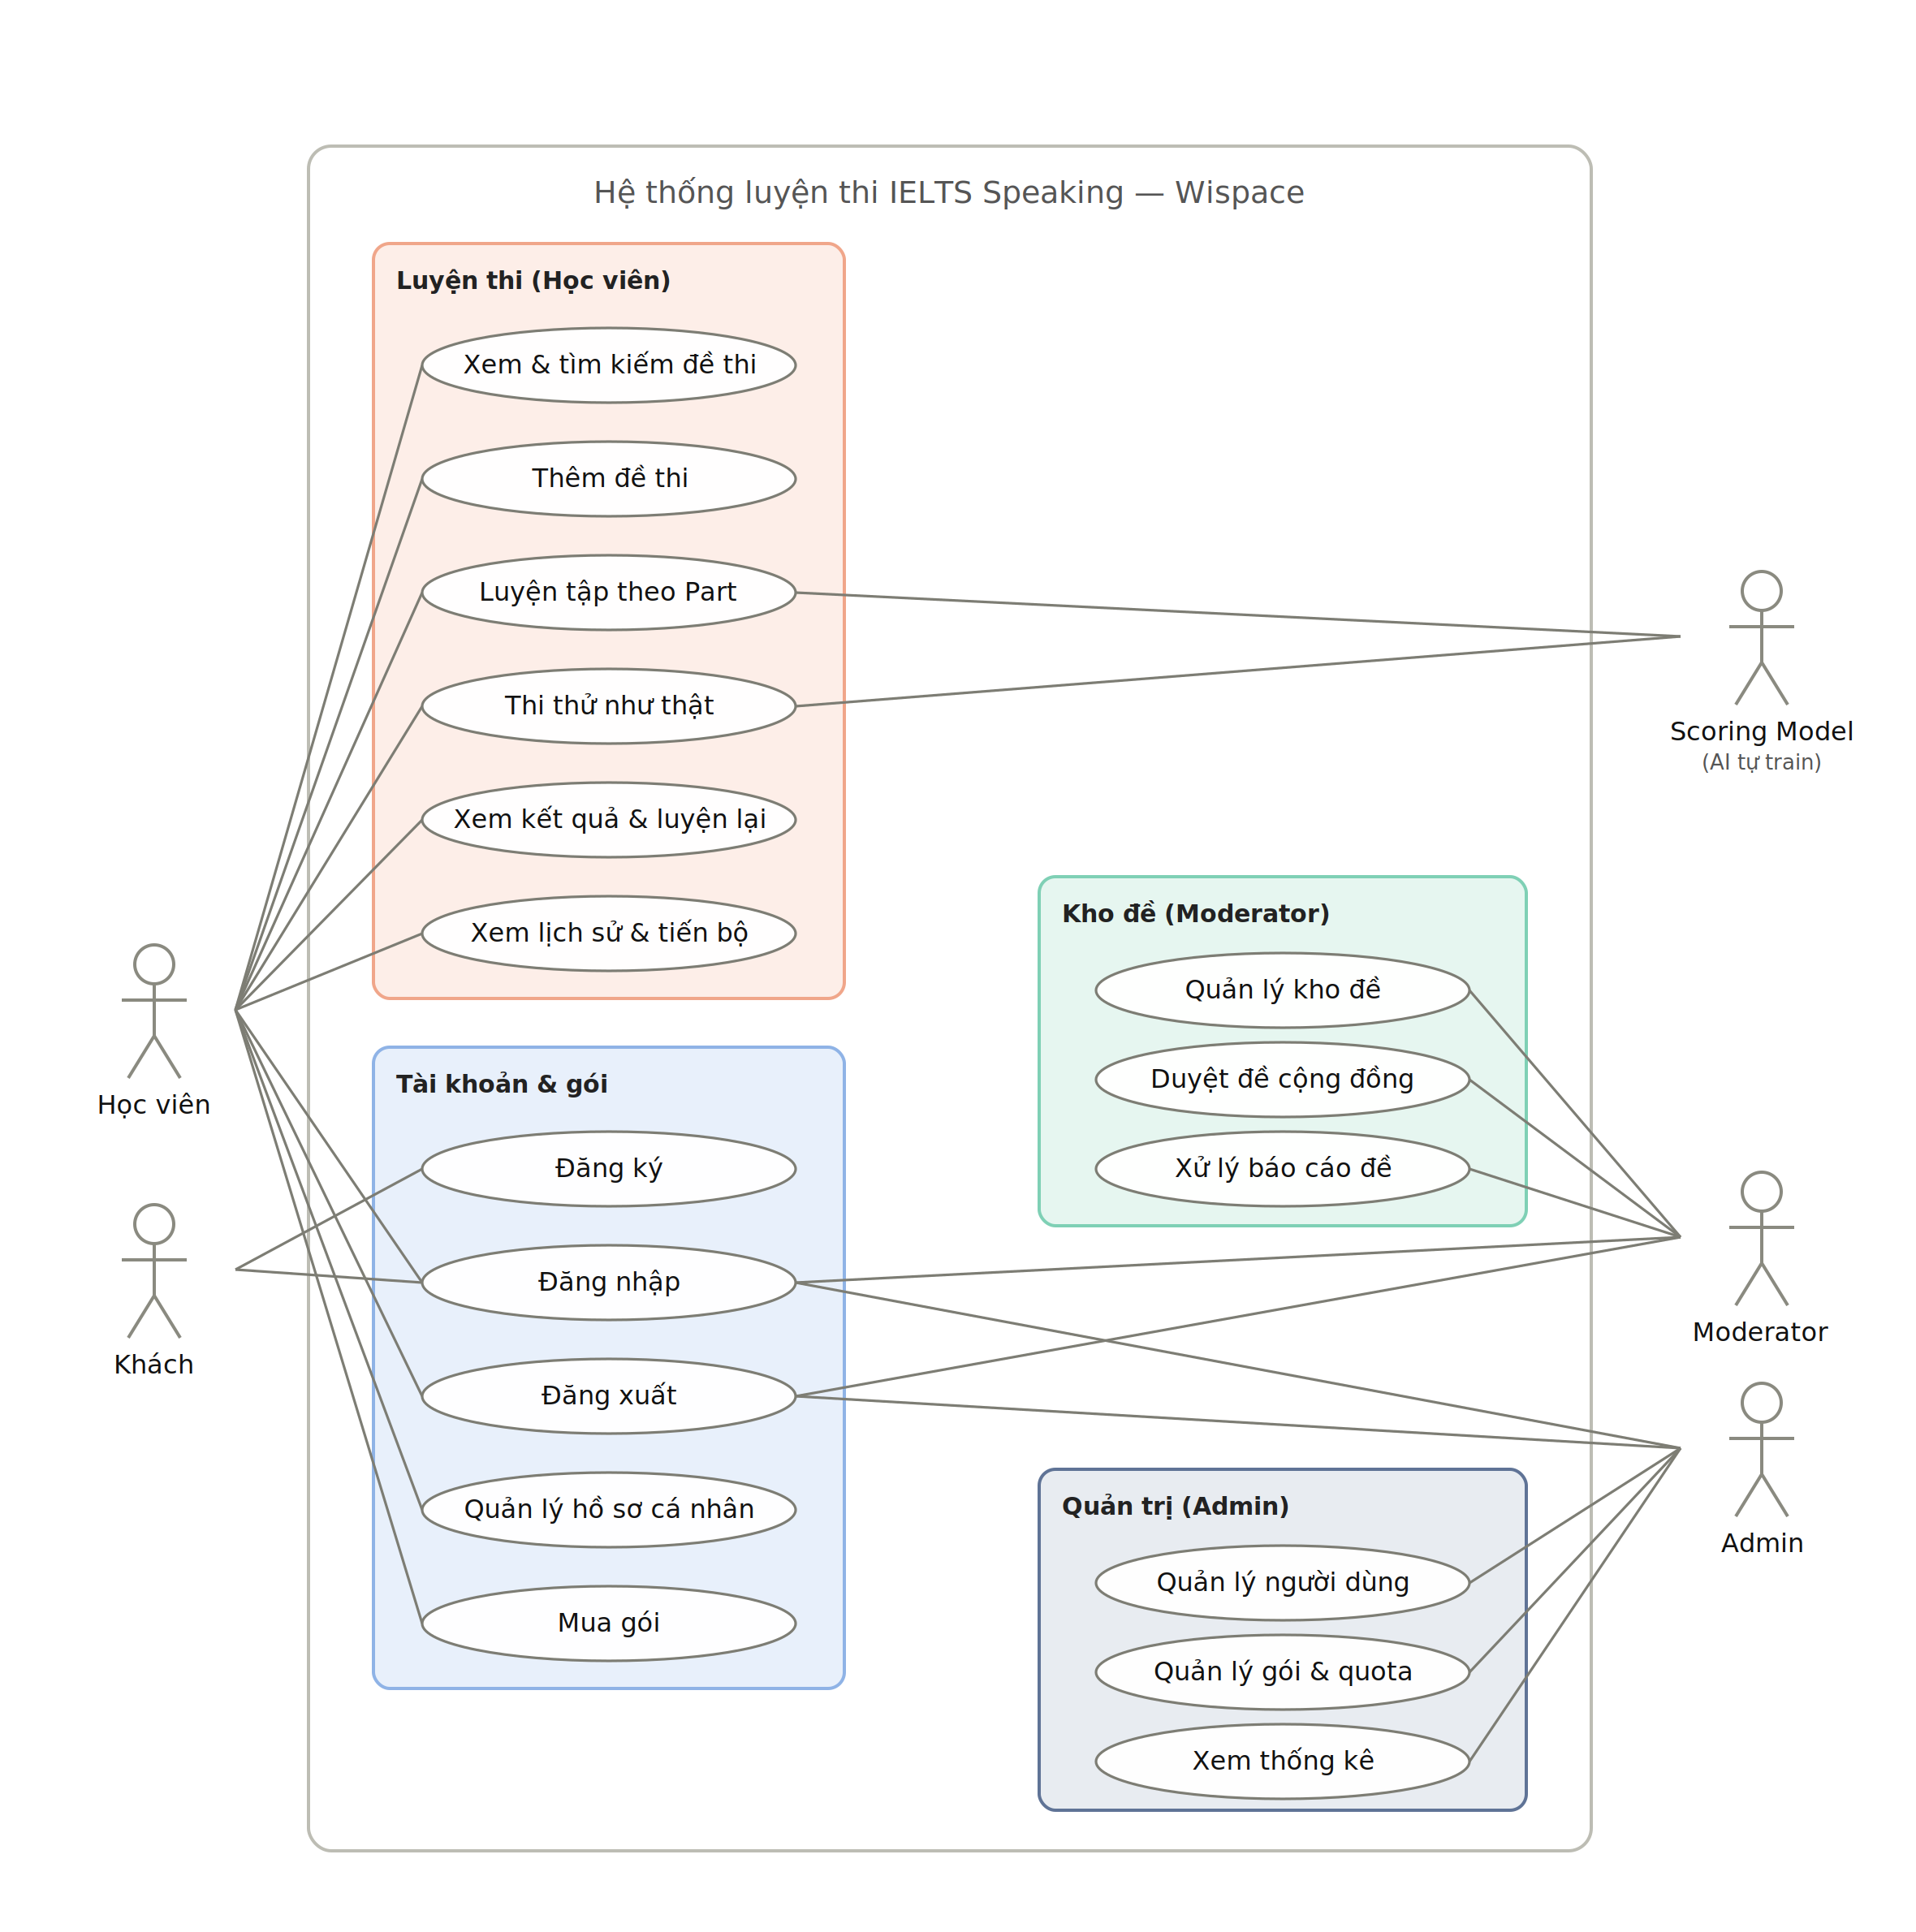
\includegraphics[width=1\textwidth]{Images/Usecase/Wispace/wispace_usecase.jpg}
    \caption{Sơ đồ Use-case tổng quan hệ thống Wispace}
    \label{wispace:fig:wispace_usecase_overview}
\end{figure}
\newpage

\subsubsection{Đặc tả các Use-case chi tiết}
\setcounter{paragraph}{0}
\renewcommand{\theparagraph}{\alph{paragraph}}

Các use-case dưới đây mô tả chi tiết những luồng nghiệp vụ cốt lõi của mô-đun Wispace Speaking, bao gồm quản lý tài khoản, quản lý kho đề, luyện tập, thi thử và theo dõi tiến bộ. Mỗi use-case xác định tác nhân, điều kiện thực hiện, luồng chính, luồng thay thế và các trường hợp ngoại lệ.

\paragraph{Use-case 1: Đăng ký tài khoản}

\begingroup
\small
\renewcommand{\arraystretch}{1.15}
\begin{longtable}{|p{3.2cm}|p{\dimexpr\linewidth-3.2cm-4\tabcolsep-3\arrayrulewidth\relax}|}
\caption{Đặc tả use-case Đăng ký tài khoản}\label{wispace:tab:wispace_uc01_register}\\
\hline
\textbf{Thuộc tính} & \textbf{Nội dung} \\ \hline
\endfirsthead
\multicolumn{2}{c}{\textit{Đặc tả use-case Đăng ký tài khoản (tiếp theo)}}\\
\hline
\textbf{Thuộc tính} & \textbf{Nội dung} \\ \hline
\endhead
\hline
\endfoot
\textbf{Tác nhân} & Khách; Dịch vụ Email; Google OAuth \\ \hline
\textbf{Tiền điều kiện} & \textbullet{}\ Hệ thống hoạt động bình thường.\newline \textbullet{}\ Khách chưa đăng nhập; email chưa tồn tại trong hệ thống. \\ \hline
\textbf{Hậu điều kiện} & \textbullet{}\ Tài khoản ở trạng thái Active, được cấp gói dùng thử.\newline \textbullet{}\ Khách được đăng nhập và chuyển tới trang onboarding. \\ \hline
\textbf{Luồng chính} & 1. Khách nhấn "Đăng ký".\newline 2. Hệ thống hiển thị form đăng ký.\newline 3. Khách nhập email, mật khẩu, xác nhận mật khẩu, nhấn "Đăng ký".\newline 4. Hệ thống kiểm tra dữ liệu, tạo tài khoản chờ xác thực và gửi OTP 6 số qua Dịch vụ Email.\newline 5. Khách nhập OTP.\newline 6. Hệ thống xác thực OTP, kích hoạt tài khoản và cấp gói dùng thử.\newline 7. Hệ thống đăng nhập và chuyển Khách tới trang onboarding. \\ \hline
\textbf{Luồng thay thế} & \textbf{Nhánh 2:} Tại bước 3 --- đăng ký bằng Google\newline 3.1. Khách nhấn "Tiếp tục với Google".\newline 3.2. Google OAuth xác thực và trả về email.\newline 3.3. Hệ thống tạo tài khoản Active, bỏ qua bước 4--6 và sang bước 7. \\ \hline
\textbf{Ngoại lệ} & \textbf{Lỗi 1:} Tại bước 4 --- email đã tồn tại: hệ thống báo lỗi, gợi ý đăng nhập hoặc quên mật khẩu.\newline \textbf{Lỗi 2:} Tại bước 4 --- mật khẩu dưới 8 ký tự hoặc không khớp: báo lỗi tại trường, giữ dữ liệu đã nhập.\newline \textbf{Lỗi 3:} Tại bước 6 --- OTP sai: cho nhập lại; sai 5 lần thì khóa 15 phút.\newline \textbf{Lỗi 4:} Tại bước 6 --- OTP quá 15 phút: Khách nhấn "Gửi lại OTP" (cách nhau tối thiểu 60 giây). \\ \hline
\end{longtable}
\endgroup


\paragraph{Use-case 2: Đăng nhập}

\begingroup
\small
\renewcommand{\arraystretch}{1.15}
\begin{longtable}{|p{3.2cm}|p{\dimexpr\linewidth-3.2cm-4\tabcolsep-3\arrayrulewidth\relax}|}
\caption{Đặc tả use-case Đăng nhập}\label{wispace:tab:wispace_uc02_login}\\
\hline
\textbf{Thuộc tính} & \textbf{Nội dung} \\ \hline
\endfirsthead
\multicolumn{2}{c}{\textit{Đặc tả use-case Đăng nhập (tiếp theo)}}\\
\hline
\textbf{Thuộc tính} & \textbf{Nội dung} \\ \hline
\endhead
\hline
\endfoot
\textbf{Tác nhân} & Học viên, Moderator, Admin; Máy chủ xác thực; Google OAuth \\ \hline
\textbf{Tiền điều kiện} & \textbullet{}\ Hệ thống hoạt động bình thường.\newline \textbullet{}\ Người dùng truy cập trang đăng nhập và đã có tài khoản. \\ \hline
\textbf{Hậu điều kiện} & \textbullet{}\ Người dùng đăng nhập thành công, nhận access token và refresh token.\newline \textbullet{}\ Người dùng được chuyển tới trang chủ theo vai trò. \\ \hline
\textbf{Luồng chính} & 1. Người dùng nhấn "Đăng nhập".\newline 2. Hệ thống hiển thị form đăng nhập.\newline 3. Người dùng nhập email, mật khẩu và nhấn "Đăng nhập".\newline 4. Máy chủ xác thực kiểm tra thông tin và trạng thái tài khoản.\newline 5. Hệ thống cấp token và chuyển trang: Học viên $\rightarrow$ Dashboard Speaking; Moderator $\rightarrow$ Quản lý đề; Admin $\rightarrow$ Trang quản trị.\newline 6. Nếu học viên có bài thi đang dở (dưới 30 phút), hệ thống hỏi "Tiếp tục bài thi" hoặc "Nộp phần đã làm". \\ \hline
\textbf{Luồng thay thế} & \textbf{Nhánh 1:} Tại bước 3 --- quên mật khẩu\newline 3.1. Người dùng nhấn "Quên mật khẩu".\newline 3.2. Hệ thống yêu cầu nhập email.\newline 3.3. Người dùng nhập email.\newline 3.4. Hệ thống gửi OTP đến email.\newline 3.5. Người dùng nhập OTP và mật khẩu mới.\newline 3.6. Hệ thống cập nhật mật khẩu, thu hồi mọi phiên cũ, quay lại bước 1.\newline \textbf{Nhánh 2:} Tại bước 3 --- đăng nhập bằng Google\newline 3.1. Người dùng nhấn "Đăng nhập bằng Google".\newline 3.2. Google OAuth xác thực và trả về email.\newline 3.3. Hệ thống sang bước 5; email chưa có tài khoản thì tự tạo tài khoản học viên. \\ \hline
\textbf{Ngoại lệ} & \textbf{Lỗi 1:} Tại bước 4 --- sai email hoặc mật khẩu: thông báo chung "Email hoặc mật khẩu không đúng"; sai 5 lần thì khóa 15 phút.\newline \textbf{Lỗi 2:} Tại bước 4 --- tài khoản bị khóa: thông báo lý do và cách liên hệ hỗ trợ.\newline \textbf{Lỗi 3:} Tại bước 4 --- tài khoản chưa xác thực OTP: gửi lại OTP và chuyển sang bước 5 của use-case Đăng ký.\newline \textbf{Lỗi 4:} Tại Alternative 1 --- email không tồn tại: vẫn báo "đã gửi mã" để không lộ thông tin tài khoản. \\ \hline
\end{longtable}
\endgroup


\paragraph{Use-case 3: Đăng xuất}

\begingroup
\small
\renewcommand{\arraystretch}{1.15}
\begin{longtable}{|p{3.2cm}|p{\dimexpr\linewidth-3.2cm-4\tabcolsep-3\arrayrulewidth\relax}|}
\caption{Đặc tả use-case Đăng xuất}\label{wispace:tab:wispace_uc03_logout}\\
\hline
\textbf{Thuộc tính} & \textbf{Nội dung} \\ \hline
\endfirsthead
\multicolumn{2}{c}{\textit{Đặc tả use-case Đăng xuất (tiếp theo)}}\\
\hline
\textbf{Thuộc tính} & \textbf{Nội dung} \\ \hline
\endhead
\hline
\endfoot
\textbf{Tác nhân} & Học viên, Moderator, Admin \\ \hline
\textbf{Tiền điều kiện} & Người dùng đã đăng nhập. \\ \hline
\textbf{Hậu điều kiện} & \textbullet{}\ Refresh token bị thu hồi; dữ liệu phiên trên trình duyệt bị xóa.\newline \textbullet{}\ Người dùng ở trang đăng nhập. \\ \hline
\textbf{Luồng chính} & 1. Người dùng nhấn "Đăng xuất".\newline 2. Hệ thống kiểm tra người dùng có đang thi hoặc đang ghi âm không.\newline 3. Hệ thống thu hồi refresh token (đưa vào danh sách chặn).\newline 4. Trình duyệt xóa token và dữ liệu tạm.\newline 5. Hệ thống chuyển về trang đăng nhập. \\ \hline
\textbf{Luồng thay thế} & \textbf{Nhánh 1:} Tại bước 1 --- đăng xuất mọi thiết bị\newline 1.1. Người dùng vào Cài đặt và nhấn "Đăng xuất mọi thiết bị".\newline 1.2. Hệ thống yêu cầu xác nhận bằng mật khẩu.\newline 1.3. Hệ thống đổi Security Stamp; mọi token cũ bị từ chối ở lần gọi tiếp theo; sang bước 4.\newline \textbf{Nhánh 2:} Tại bước 2 --- đang trong phòng thi\newline 2.1. Hệ thống hiển thị hộp thoại: "Nộp phần đã làm và đăng xuất" / "Huỷ bài thi" / "Quay lại".\newline 2.2. Chọn nộp: hệ thống lưu bài, đưa vào hàng chấm và sang bước 3.\newline 2.3. Chọn quay lại: kết thúc use-case, tiếp tục thi. \\ \hline
\textbf{Ngoại lệ} & \textbf{Lỗi 1:} Tại bước 3 --- mất mạng: trình duyệt vẫn xóa token cục bộ; refresh token tự hết hạn.\newline \textbf{Lỗi 2:} Tại bước 2 --- còn audio chưa upload: cảnh báo và chờ upload xong mới đăng xuất. \\ \hline
\end{longtable}
\endgroup


\paragraph{Use-case 4: Quản lý hồ sơ cá nhân}

\begingroup
\small
\renewcommand{\arraystretch}{1.15}
\begin{longtable}{|p{3.2cm}|p{\dimexpr\linewidth-3.2cm-4\tabcolsep-3\arrayrulewidth\relax}|}
\caption{Đặc tả use-case Quản lý hồ sơ cá nhân}\label{wispace:tab:wispace_uc04_profile}\\
\hline
\textbf{Thuộc tính} & \textbf{Nội dung} \\ \hline
\endfirsthead
\multicolumn{2}{c}{\textit{Đặc tả use-case Quản lý hồ sơ cá nhân (tiếp theo)}}\\
\hline
\textbf{Thuộc tính} & \textbf{Nội dung} \\ \hline
\endhead
\hline
\endfoot
\textbf{Tác nhân} & Học viên \\ \hline
\textbf{Tiền điều kiện} & Học viên đã đăng nhập. \\ \hline
\textbf{Hậu điều kiện} & \textbullet{}\ Thông tin hồ sơ được lưu.\newline \textbullet{}\ Band mục tiêu và ngày thi được dùng để cá nhân hoá gợi ý luyện tập. \\ \hline
\textbf{Luồng chính} & 1. Học viên nhấn "Hồ sơ".\newline 2. Hệ thống hiển thị 4 tab: Thông tin, Thiết bị, Gói \& quota, Quyền riêng tư.\newline 3. Học viên sửa tên, avatar, band mục tiêu (5.0--9.0), ngày thi dự kiến, giọng giám khảo (Anh-Anh / Anh-Mỹ / Úc) và nhấn "Lưu".\newline 4. Hệ thống kiểm tra dữ liệu và lưu.\newline 5. Hệ thống thông báo cập nhật thành công. \\ \hline
\textbf{Luồng thay thế} & \textbf{Nhánh 1:} Tại bước 2 --- kiểm tra micro\newline 2.1. Học viên chọn tab Thiết bị, chọn micro và ghi thử 5 giây.\newline 2.2. Hệ thống phát lại và hiển thị mức âm lượng, độ ồn.\newline \textbf{Nhánh 2:} Tại bước 2 --- đổi mật khẩu\newline 2.1. Học viên nhập mật khẩu cũ và mật khẩu mới.\newline 2.2. Hệ thống cập nhật và thu hồi phiên trên các thiết bị khác.\newline \textbf{Nhánh 3:} Tại bước 2 --- xem gói \& quota\newline 2.1. Hệ thống hiển thị gói hiện tại, ngày hết hạn, số phút chấm và lượt thi còn lại hôm nay.\newline 2.2. Học viên nhấn "Nâng cấp" để chuyển sang use-case Mua gói.\newline \textbf{Nhánh 4:} Tại bước 2 --- xóa audio / xóa tài khoản\newline 2.1. Học viên chọn tab Quyền riêng tư, nhấn xóa và xác nhận bằng mật khẩu hoặc OTP.\newline 2.2. Hệ thống xóa audio ngay; với xóa tài khoản, chuyển sang trạng thái Chờ xóa 30 ngày và đăng xuất mọi thiết bị. \\ \hline
\textbf{Ngoại lệ} & \textbf{Lỗi 1:} Tại bước 4 --- ảnh avatar lớn hơn 2 MB hoặc sai định dạng: báo lỗi, không lưu ảnh.\newline \textbf{Lỗi 2:} Tại Alternative 1 --- trình duyệt chặn micro: hướng dẫn cấp quyền theo từng trình duyệt.\newline \textbf{Lỗi 3:} Tại Alternative 2 --- mật khẩu cũ sai: báo lỗi, không đổi mật khẩu. \\ \hline
\end{longtable}
\endgroup


\paragraph{Use-case 5: Quản lý người dùng}

\begingroup
\small
\renewcommand{\arraystretch}{1.15}
\begin{longtable}{|p{3.2cm}|p{\dimexpr\linewidth-3.2cm-4\tabcolsep-3\arrayrulewidth\relax}|}
\caption{Đặc tả use-case Quản lý người dùng}\label{wispace:tab:wispace_uc05_user_management}\\
\hline
\textbf{Thuộc tính} & \textbf{Nội dung} \\ \hline
\endfirsthead
\multicolumn{2}{c}{\textit{Đặc tả use-case Quản lý người dùng (tiếp theo)}}\\
\hline
\textbf{Thuộc tính} & \textbf{Nội dung} \\ \hline
\endhead
\hline
\endfoot
\textbf{Tác nhân} & Admin; Dịch vụ Email \\ \hline
\textbf{Tiền điều kiện} & Admin đã đăng nhập với vai trò Admin. \\ \hline
\textbf{Hậu điều kiện} & \textbullet{}\ Thay đổi có hiệu lực ngay.\newline \textbullet{}\ Mỗi thao tác được ghi nhật ký (người làm, thời điểm, trước/sau, lý do).\newline \textbullet{}\ Người dùng nhận email thông báo. \\ \hline
\textbf{Luồng chính} & 1. Admin mở "Quản lý người dùng".\newline 2. Hệ thống hiển thị danh sách phân trang 20 dòng và bộ lọc.\newline 3. Admin nhập email/tên và lọc theo vai trò, gói, trạng thái, ngày đăng ký.\newline 4. Hệ thống trả kết quả.\newline 5. Admin chọn một người dùng.\newline 6. Hệ thống hiển thị chi tiết: thông tin, gói, lịch sử thanh toán, quota đã dùng 30 ngày, số bài, band trung bình.\newline 7. Admin chọn thao tác (Khóa / mở khóa, Đổi vai trò, Cộng quota), nhập lý do và xác nhận.\newline 8. Hệ thống áp dụng thay đổi, ghi nhật ký và gửi email thông báo qua Dịch vụ Email. \\ \hline
\textbf{Luồng thay thế} & \textbf{Nhánh 1:} Tại bước 7 --- khóa tài khoản\newline 7.1. Hệ thống đổi Security Stamp, người dùng bị đăng xuất ngay.\newline 7.2. Bài thi đang làm (nếu có) được lưu ở trạng thái Đã huỷ.\newline \textbf{Nhánh 2:} Tại bước 7 --- cộng quota thủ công\newline 7.1. Admin nhập số phút chấm hoặc số lượt thi và hạn dùng.\newline 7.2. Hệ thống tạo bản ghi điều chỉnh quota.\newline \textbf{Nhánh 3:} Tại bước 4 --- xuất danh sách\newline 4.1. Admin nhấn "Xuất CSV"; hệ thống tải file theo bộ lọc hiện tại. \\ \hline
\textbf{Ngoại lệ} & \textbf{Lỗi 1:} Tại bước 4 --- không có kết quả: hiển thị "Không tìm thấy người dùng".\newline \textbf{Lỗi 2:} Tại bước 6 --- xem audio của người dùng: chỉ mở khi nhập mã ticket hỗ trợ; hệ thống ghi nhật ký.\newline \textbf{Lỗi 3:} Tại bước 7 --- không nhập lý do: không cho xác nhận.\newline \textbf{Lỗi 4:} Tại bước 7 --- Admin khóa hoặc hạ vai trò chính mình: hệ thống từ chối. \\ \hline
\end{longtable}
\endgroup


\paragraph{Use-case 6: Xem và tìm kiếm đề thi}

\begingroup
\small
\renewcommand{\arraystretch}{1.15}
\begin{longtable}{|p{3.2cm}|p{\dimexpr\linewidth-3.2cm-4\tabcolsep-3\arrayrulewidth\relax}|}
\caption{Đặc tả use-case Xem và tìm kiếm đề thi}\label{wispace:tab:wispace_uc06_browse_tests}\\
\hline
\textbf{Thuộc tính} & \textbf{Nội dung} \\ \hline
\endfirsthead
\multicolumn{2}{c}{\textit{Đặc tả use-case Xem và tìm kiếm đề thi (tiếp theo)}}\\
\hline
\textbf{Thuộc tính} & \textbf{Nội dung} \\ \hline
\endhead
\hline
\endfoot
\textbf{Tác nhân} & Học viên, Khách \\ \hline
\textbf{Tiền điều kiện} & \textbullet{}\ Hệ thống hoạt động bình thường.\newline \textbullet{}\ Kho đề có dữ liệu. \\ \hline
\textbf{Hậu điều kiện} & Người dùng thấy danh sách hoặc chi tiết đề; học viên có thể chuyển sang Luyện tập hoặc Thi thử. \\ \hline
\textbf{Luồng chính} & 1. Người dùng nhấn "Đề thi Speaking".\newline 2. Hệ thống hiển thị các tab nguồn (Cambridge, Forecast, Đề của tôi, Cộng đồng), mặc định Forecast quý hiện tại, 24 thẻ mỗi trang.\newline 3. Người dùng chọn tab, lọc theo Part, chủ đề, trạng thái hoặc nhập từ khoá.\newline 4. Hệ thống trả về các đề phù hợp.\newline 5. Người dùng nhấn vào một thẻ đề.\newline 6. Hệ thống hiển thị chi tiết: câu hỏi từng Part, số lượt luyện, band cao nhất của học viên, nút "Luyện tập" và "Thi thử". \\ \hline
\textbf{Luồng thay thế} & \textbf{Nhánh 1:} Tại bước 3 --- chọn tab Cambridge\newline 3.1. Hệ thống hiển thị lưới quyển Cambridge IELTS 1--20.\newline 3.2. Người dùng chọn quyển; hệ thống hiển thị Test 1--4 của quyển đó, sang bước 5.\newline \textbf{Nhánh 2:} Tại bước 6 --- đánh dấu yêu thích\newline 6.1. Học viên nhấn biểu tượng ngôi sao; hệ thống lưu đề vào danh sách Yêu thích.\newline \textbf{Nhánh 3:} Tại bước 6 --- báo cáo đề sai\newline 6.1. Học viên chọn lý do (sai nội dung, trùng, không phù hợp) và gửi.\newline 6.2. Hệ thống đưa báo cáo vào hàng chờ của Moderator. \\ \hline
\textbf{Ngoại lệ} & \textbf{Lỗi 1:} Tại bước 4 --- không có kết quả: gợi ý bỏ bớt bộ lọc hoặc "Thêm đề này".\newline \textbf{Lỗi 2:} Tại bước 6 --- Khách nhấn Luyện tập / Thi thử: chuyển sang use-case Đăng nhập.\newline \textbf{Lỗi 3:} Tại bước 6 --- đề thuộc gói trả phí, học viên dùng gói miễn phí: hiển thị màn hình nâng cấp gói.\newline \textbf{Lỗi 4:} Tại bước 3 --- tab Đề của tôi trống: hiển thị nút "Thêm đề đầu tiên". \\ \hline
\end{longtable}
\endgroup


\paragraph{Use-case 7: Thêm đề thi}

\begingroup
\small
\renewcommand{\arraystretch}{1.15}
\begin{longtable}{|p{3.2cm}|p{\dimexpr\linewidth-3.2cm-4\tabcolsep-3\arrayrulewidth\relax}|}
\caption{Đặc tả use-case Thêm đề thi}\label{wispace:tab:wispace_uc07_add_test}\\
\hline
\textbf{Thuộc tính} & \textbf{Nội dung} \\ \hline
\endfirsthead
\multicolumn{2}{c}{\textit{Đặc tả use-case Thêm đề thi (tiếp theo)}}\\
\hline
\textbf{Thuộc tính} & \textbf{Nội dung} \\ \hline
\endhead
\hline
\endfoot
\textbf{Tác nhân} & Học viên; AI hỗ trợ \\ \hline
\textbf{Tiền điều kiện} & \textbullet{}\ Học viên đã đăng nhập.\newline \textbullet{}\ Chưa vượt giới hạn số đề (gói miễn phí 10 đề, gói trả phí 200 đề). \\ \hline
\textbf{Hậu điều kiện} & \textbullet{}\ Đề được lưu ở chế độ Riêng tư, nguồn "Học viên tạo".\newline \textbullet{}\ Đề hiển thị trong tab Đề của tôi và luyện được ngay. \\ \hline
\textbf{Luồng chính} & 1. Học viên nhấn "+ Thêm đề".\newline 2. Hệ thống hiển thị form chọn loại đề: Part 1, Part 2 (kèm Part 3), Full test.\newline 3. Học viên nhập nội dung (Part 1: chủ đề + 3--6 câu; Part 2: cue card + 3--4 gợi ý; Part 3: 4--6 câu thảo luận), gắn chủ đề, nguồn tham khảo và nhấn "Lưu".\newline 4. Hệ thống kiểm tra hợp lệ: mỗi câu tối đa 300 ký tự, bằng tiếng Anh, lọc từ ngữ không phù hợp, loại bỏ mã HTML.\newline 5. Hệ thống kiểm tra trùng lặp với kho đề.\newline 6. Hệ thống lưu đề và hiển thị nút "Luyện ngay" và "Đề xuất công khai". \\ \hline
\textbf{Luồng thay thế} & \textbf{Nhánh 1:} Tại bước 3 --- AI gợi ý câu Part 3\newline 3.1. Học viên nhập cue card Part 2 và nhấn "Gợi ý Part 3".\newline 3.2. AI hỗ trợ sinh 5 câu Part 3 liên quan.\newline 3.3. Học viên giữ hoặc bỏ từng câu, quay lại bước 3.\newline \textbf{Nhánh 2:} Tại bước 5 --- đề gần giống đề có sẵn (từ 90\%)\newline 5.1. Hệ thống hiển thị đề có sẵn.\newline 5.2. Học viên chọn "Dùng đề có sẵn" (kết thúc) hoặc "Vẫn lưu" (sang bước 6).\newline \textbf{Nhánh 3:} Tại bước 6 --- đề xuất công khai\newline 6.1. Học viên nhấn "Đề xuất công khai".\newline 6.2. Hệ thống chuyển đề sang trạng thái Chờ duyệt và đưa vào hàng chờ Moderator (use-case 5.8). \\ \hline
\textbf{Ngoại lệ} & \textbf{Lỗi 1:} Tại bước 1 --- vượt giới hạn số đề: thông báo và gợi ý nâng cấp gói.\newline \textbf{Lỗi 2:} Tại bước 4 --- dữ liệu không hợp lệ: báo lỗi đúng trường, giữ dữ liệu đã nhập.\newline \textbf{Lỗi 3:} Tại Alternative 1 --- AI lỗi hoặc quá 30 giây: báo lỗi, học viên tự nhập Part 3. \\ \hline
\end{longtable}
\endgroup


\paragraph{Use-case 8: Quản lý và duyệt kho đề}

\begingroup
\small
\renewcommand{\arraystretch}{1.15}
\begin{longtable}{|p{3.2cm}|p{\dimexpr\linewidth-3.2cm-4\tabcolsep-3\arrayrulewidth\relax}|}
\caption{Đặc tả use-case Quản lý và duyệt kho đề}\label{wispace:tab:wispace_uc08_moderate_tests}\\
\hline
\textbf{Thuộc tính} & \textbf{Nội dung} \\ \hline
\endfirsthead
\multicolumn{2}{c}{\textit{Đặc tả use-case Quản lý và duyệt kho đề (tiếp theo)}}\\
\hline
\textbf{Thuộc tính} & \textbf{Nội dung} \\ \hline
\endhead
\hline
\endfoot
\textbf{Tác nhân} & Moderator; Dịch vụ TTS \\ \hline
\textbf{Tiền điều kiện} & Người dùng đã đăng nhập với vai trò Moderator hoặc Admin. \\ \hline
\textbf{Hậu điều kiện} & \textbullet{}\ Kho đề được cập nhật; đề mới có sẵn audio câu hỏi.\newline \textbullet{}\ Tác giả đề cộng đồng nhận thông báo kết quả duyệt. \\ \hline
\textbf{Luồng chính} & 1. Moderator mở "Quản lý đề".\newline 2. Hệ thống hiển thị cây Quyển $\rightarrow$ Test $\rightarrow$ Part $\rightarrow$ Câu hỏi và hàng chờ duyệt.\newline 3. Moderator nhấn "Thêm đề", chọn Quyển/Test, nhập câu hỏi từng Part và nhấn "Lưu".\newline 4. Hệ thống kiểm tra hợp lệ và lưu đề.\newline 5. Hệ thống gửi câu hỏi tới Dịch vụ TTS để sinh audio 3 giọng (Anh-Anh, Anh-Mỹ, Úc) và lưu lại để dùng chung.\newline 6. Hệ thống hiển thị đề trên trang đề thi. \\ \hline
\textbf{Luồng thay thế} & \textbf{Nhánh 1:} Tại bước 3 --- nhập file\newline 3.1. Moderator tải lên file CSV/JSON theo mẫu.\newline 3.2. Hệ thống kiểm tra từng dòng; có lỗi thì báo dòng lỗi và không nhập phần nào; hợp lệ thì sang bước 5.\newline \textbf{Nhánh 2:} Tại bước 3 --- tạo bộ Forecast quý\newline 3.1. Moderator chọn các đề Part 1/2/3 và đặt thời gian hiệu lực (ví dụ 01/09--31/12/2026).\newline 3.2. Hệ thống lưu bộ Forecast và sang bước 6.\newline \textbf{Nhánh 3:} Tại bước 2 --- duyệt đề cộng đồng\newline 2.1. Moderator mở một đề chờ duyệt; hệ thống hiển thị kèm các đề tương tự.\newline 2.2. Moderator chọn Duyệt (có thể sửa chính tả, gắn tag), Từ chối (bắt buộc ghi lý do) hoặc Gộp trùng.\newline 2.3. Hệ thống cập nhật trạng thái đề và thông báo cho tác giả.\newline \textbf{Nhánh 4:} Tại bước 2 --- xử lý báo cáo đề\newline 2.1. Moderator mở báo cáo và chọn Gỡ đề, Sửa đề hoặc Bỏ qua.\newline 2.2. Tác giả bị gỡ từ 3 đề trong 30 ngày thì bị tạm khóa quyền đề xuất 30 ngày và Admin nhận thông báo. \\ \hline
\textbf{Ngoại lệ} & \textbf{Lỗi 1:} Tại bước 4 --- thiếu câu hỏi bắt buộc: báo lỗi, không lưu.\newline \textbf{Lỗi 2:} Tại bước 5 --- Dịch vụ TTS lỗi: đề vẫn được lưu, đánh dấu "Thiếu audio" và tự sinh lại sau.\newline \textbf{Lỗi 3:} Tại bước 3 --- ẩn đề đã có bài làm: đề không còn trong danh sách nhưng lịch sử bài của học viên vẫn xem được. \\ \hline
\end{longtable}
\endgroup


\paragraph{Use-case 9: Luyện tập theo Part}

\begingroup
\small
\renewcommand{\arraystretch}{1.15}
\begin{longtable}{|p{3.2cm}|p{\dimexpr\linewidth-3.2cm-4\tabcolsep-3\arrayrulewidth\relax}|}
\caption{Đặc tả use-case Luyện tập theo Part}\label{wispace:tab:wispace_uc09_part_practice}\\
\hline
\textbf{Thuộc tính} & \textbf{Nội dung} \\ \hline
\endfirsthead
\multicolumn{2}{c}{\textit{Đặc tả use-case Luyện tập theo Part (tiếp theo)}}\\
\hline
\textbf{Thuộc tính} & \textbf{Nội dung} \\ \hline
\endhead
\hline
\endfoot
\textbf{Tác nhân} & Học viên; Scoring Model (AI chấm tự train) \\ \hline
\textbf{Tiền điều kiện} & \textbullet{}\ Học viên đã đăng nhập và đã cấp quyền micro.\newline \textbullet{}\ Còn quota phút chấm trong ngày. \\ \hline
\textbf{Hậu điều kiện} & \textbullet{}\ Bài làm, audio, transcript và kết quả được lưu.\newline \textbullet{}\ Quota bị trừ theo số giây audio; sự kiện luyện tập được gửi tới hệ thống thống kê. \\ \hline
\textbf{Luồng chính} & 1. Học viên nhấn "Luyện tập".\newline 2. Hệ thống kiểm tra quota và tạo phiên luyện tập.\newline 3. Hệ thống hiển thị câu hỏi (chữ và nút nghe).\newline 4. Học viên nhấn ghi âm (hoặc phím Space) và trả lời; hệ thống ghi và tải audio lên theo từng đoạn.\newline 5. Học viên nhấn dừng, nghe lại và nhấn "Nộp".\newline 6. Hệ thống gửi audio tới Scoring Model; model trả transcript, lỗi phát âm từng từ và band 4 tiêu chí.\newline 7. Hệ thống hiển thị trạng thái "Đang phân tích" $\rightarrow$ "Đang chấm" $\rightarrow$ kết quả (use-case 5.10).\newline 8. Học viên chuyển sang câu tiếp theo. \\ \hline
\textbf{Luồng thay thế} & \textbf{Nhánh 1:} Tại bước 3 --- nghe câu hỏi\newline 3.1. Học viên nhấn biểu tượng loa; hệ thống phát audio câu hỏi; có thể ẩn chữ để luyện nghe.\newline \textbf{Nhánh 2:} Tại bước 3 --- câu hỏi Part 2\newline 3.1. Hệ thống hiển thị cue card, giấy nháp và đếm 60 giây chuẩn bị.\newline 3.2. Hết 60 giây (hoặc nhấn "Bắt đầu nói sớm"), hệ thống tự ghi âm tối đa 120 giây, sang bước 5.\newline \textbf{Nhánh 3:} Tại bước 5 --- ghi lại\newline 5.1. Học viên nhấn "Ghi lại"; bản cũ bị thay, không trừ quota; quay lại bước 4. \\ \hline
\textbf{Ngoại lệ} & \textbf{Lỗi 1:} Tại bước 2 --- hết quota: hiển thị số phút đã dùng, giờ reset và nút nâng cấp; vẫn cho ghi âm tự nghe nhưng không chấm.\newline \textbf{Lỗi 2:} Tại bước 4 --- micro bị chặn: hướng dẫn cấp quyền; nói quá 3 phút (Part 1/3) thì tự dừng.\newline \textbf{Lỗi 3:} Tại bước 5 --- audio dưới 3 giây hoặc im lặng hơn 80\%: không cho nộp, báo "Không nghe rõ câu trả lời".\newline \textbf{Lỗi 4:} Tại bước 6 --- phần lớn nói tiếng Việt: không chấm, hoàn quota.\newline \textbf{Lỗi 5:} Tại bước 6 --- AI lỗi hoặc quá 60 giây: thực thi tối đa 3 lần (gồm lần đầu); vẫn lỗi thì đánh dấu Thất bại, hoàn quota và cho nhấn "Chấm lại". \\ \hline
\end{longtable}
\endgroup


\paragraph{Use-case 10: Xem kết quả và luyện lại}

\begingroup
\small
\renewcommand{\arraystretch}{1.15}
\begin{longtable}{|p{3.2cm}|p{\dimexpr\linewidth-3.2cm-4\tabcolsep-3\arrayrulewidth\relax}|}
\caption{Đặc tả use-case Xem kết quả và luyện lại}\label{wispace:tab:wispace_uc10_results_retry}\\
\hline
\textbf{Thuộc tính} & \textbf{Nội dung} \\ \hline
\endfirsthead
\multicolumn{2}{c}{\textit{Đặc tả use-case Xem kết quả và luyện lại (tiếp theo)}}\\
\hline
\textbf{Thuộc tính} & \textbf{Nội dung} \\ \hline
\endhead
\hline
\endfoot
\textbf{Tác nhân} & Học viên \\ \hline
\textbf{Tiền điều kiện} & \textbullet{}\ Học viên đã đăng nhập.\newline \textbullet{}\ Câu trả lời đã được chấm thành công. \\ \hline
\textbf{Hậu điều kiện} & Học viên thấy kết quả; nếu luyện lại, lượt mới được lưu và so sánh với lượt trước. \\ \hline
\textbf{Luồng chính} & 1. Học viên mở trang kết quả.\newline 2. Hệ thống hiển thị band tổng và 4 thẻ tiêu chí (FC, LR, GRA, P): điểm, lý do, điểm mạnh, điểm cần cải thiện.\newline 3. Hệ thống hiển thị transcript tô màu lỗi ngữ pháp, từ vựng, phát âm và chỉ số trôi chảy (số từ/phút, số lần ngập ngừng, từ đệm).\newline 4. Học viên đọc nhận xét và gợi ý bước tiếp theo. \\ \hline
\textbf{Luồng thay thế} & \textbf{Nhánh 1:} Tại bước 3 --- nghe lại từ phát âm sai\newline 3.1. Học viên nhấn vào từ được tô.\newline 3.2. Hệ thống phát đoạn audio của học viên, sau đó phát âm chuẩn kèm phiên âm IPA.\newline \textbf{Nhánh 2:} Tại bước 4 --- xem câu trả lời mẫu\newline 4.1. Hệ thống hiển thị câu trả lời band 7.0+ viết lại từ ý của học viên và danh sách từ vựng nâng cấp.\newline \textbf{Nhánh 3:} Tại bước 4 --- luyện lại câu này\newline 4.1. Học viên nhấn "Luyện lại câu này"; hệ thống chuyển sang use-case 5.9 với cùng câu hỏi.\newline 4.2. Chấm xong, hệ thống hiển thị so sánh lần trước và lần này theo 4 tiêu chí.\newline \textbf{Nhánh 4:} Tại bước 4 --- thêm lỗi vào Roadmap\newline 4.1. Lỗi lặp lại từ 3 lần trong 14 ngày, hệ thống gợi ý "Thêm vào Roadmap".\newline 4.2. Học viên đồng ý; lỗi được thêm thành một chương luyện tập. \\ \hline
\textbf{Ngoại lệ} & \textbf{Lỗi 1:} Tại bước 1 --- bài đang chấm: hiển thị trạng thái chờ và tự cập nhật khi xong.\newline \textbf{Lỗi 2:} Tại bước 1 --- chấm thất bại: hiển thị lý do và nút "Chấm lại" (không trừ quota).\newline \textbf{Lỗi 3:} Tại Alternative 1 --- audio đã bị xóa theo chính sách 180 ngày: chỉ hiển thị transcript và phát âm chuẩn.\newline \textbf{Lỗi 4:} Tại Alternative 3 --- hết quota: xử lý như Lỗi 1 của use-case 5.9. \\ \hline
\end{longtable}
\endgroup


\paragraph{Use-case 11: Thi thử như thật}

\begingroup
\small
\renewcommand{\arraystretch}{1.15}
\begin{longtable}{|p{3.2cm}|p{\dimexpr\linewidth-3.2cm-4\tabcolsep-3\arrayrulewidth\relax}|}
\caption{Đặc tả use-case Thi thử như thật}\label{wispace:tab:wispace_uc11_mock_test}\\
\hline
\textbf{Thuộc tính} & \textbf{Nội dung} \\ \hline
\endfirsthead
\multicolumn{2}{c}{\textit{Đặc tả use-case Thi thử như thật (tiếp theo)}}\\
\hline
\textbf{Thuộc tính} & \textbf{Nội dung} \\ \hline
\endhead
\hline
\endfoot
\textbf{Tác nhân} & Học viên; Giám khảo AI; Scoring Model (AI chấm tự train) \\ \hline
\textbf{Tiền điều kiện} & \textbullet{}\ Học viên đã đăng nhập, còn lượt thi thử hôm nay.\newline \textbullet{}\ Không có phiên thi khác đang mở; thiết bị có micro. \\ \hline
\textbf{Hậu điều kiện} & \textbullet{}\ Mọi câu trả lời được lưu; bài chuyển sang Đã nộp và vào hàng chấm; trừ 1 lượt thi.\newline \textbullet{}\ Học viên nhận thông báo khi có báo cáo. \\ \hline
\textbf{Luồng chính} & 1. Học viên chọn đề và nhấn "Thi thử".\newline 2. Hệ thống hiển thị quy chế (không nghe lại, không ghi lại, không tạm dừng; khuyến nghị tai nghe) và xin đồng ý xử lý giọng nói ở lần đầu.\newline 3. Hệ thống kiểm tra thiết bị: chỉnh loa, đọc câu mẫu 5 giây để đo âm lượng và độ ồn, đo mạng.\newline 4. Học viên nhấn "Bắt đầu thi"; hệ thống tạo phiên thi, trừ 1 lượt và tải trước audio câu hỏi.\newline 5. Part 1 (4--5 phút): giám khảo AI đọc từng câu; hệ thống tự ghi âm khi giám khảo nói xong và chuyển câu khi học viên im lặng từ 3 giây hoặc hết 45 giây.\newline 6. Part 2: hệ thống hiển thị cue card và giấy nháp, đếm 60 giây chuẩn bị; giám khảo mời bắt đầu; ghi âm tối đa 120 giây rồi ngắt.\newline 7. Part 3 (4--5 phút): giám khảo hỏi 4--6 câu thảo luận liên quan đến Part 2.\newline 8. Giám khảo kết thúc; hệ thống kiểm tra mọi audio đã tải lên, chuyển bài sang Đã nộp và đưa vào hàng chấm.\newline 9. Scoring Model chấm từng câu và cả bài; hệ thống tạo báo cáo và thông báo qua ứng dụng và email. \\ \hline
\textbf{Luồng thay thế} & \textbf{Nhánh 1:} Tại bước 1 --- thi ngẫu nhiên\newline 1.1. Hệ thống ghép Part 1 + Part 2 + Part 3 cùng chủ đề từ kho đề, sang bước 2.\newline \textbf{Nhánh 2:} Tại bước 5--7 --- xin nhắc lại câu hỏi\newline 5.1. Học viên nhấn "Xin nhắc lại câu hỏi" hoặc nói "Sorry, could you repeat?".\newline 5.2. Giám khảo đọc lại 1 lần, không trừ thời gian.\newline \textbf{Nhánh 3:} Tại bước 6 --- nói dưới 60 giây rồi im lặng từ 5 giây\newline 6.1. Giám khảo hỏi gợi mở "Can you tell me more?" như thi thật.\newline \textbf{Nhánh 4:} Tại bước 5--7 --- kết thúc sớm\newline 5.1. Học viên nhấn "Kết thúc" và xác nhận.\newline 5.2. Hệ thống nộp phần đã làm, sang bước 8; báo cáo chỉ có band từng Part. \\ \hline
\textbf{Ngoại lệ} & \textbf{Lỗi 1:} Tại bước 3 --- không có micro hoặc không cấp quyền: không cho vào thi.\newline \textbf{Lỗi 2:} Tại bước 3 --- ồn nền cao hoặc mic nhỏ: cảnh báo, cho "Vẫn tiếp tục" và đánh dấu chất lượng âm thanh thấp.\newline \textbf{Lỗi 3:} Tại bước 4 --- hết lượt thi: hiển thị màn hình nâng cấp, gợi ý luyện từng Part.\newline \textbf{Lỗi 4:} Tại bước 5--7 --- mất mạng: tiếp tục ghi vào bộ nhớ trình duyệt, tải bù khi có mạng lại.\newline \textbf{Lỗi 5:} Tại bước 5--7 --- tải lại trang hoặc đóng tab: cảnh báo rời trang; quay lại trong 30 phút thì tiếp tục từ câu chưa trả lời, quá 30 phút thì tự nộp phần đã làm.\newline \textbf{Lỗi 6:} Tại bước 9 --- chấm lỗi sau 3 lần thử: bài ở trạng thái Thất bại, hoàn lượt thi và báo Admin. \\ \hline
\end{longtable}
\endgroup


\paragraph{Use-case 12: Xem lịch sử và tiến bộ}

\begingroup
\small
\renewcommand{\arraystretch}{1.15}
\begin{longtable}{|p{3.2cm}|p{\dimexpr\linewidth-3.2cm-4\tabcolsep-3\arrayrulewidth\relax}|}
\caption{Đặc tả use-case Xem lịch sử và tiến bộ}\label{wispace:tab:wispace_uc12_progress_history}\\
\hline
\textbf{Thuộc tính} & \textbf{Nội dung} \\ \hline
\endfirsthead
\multicolumn{2}{c}{\textit{Đặc tả use-case Xem lịch sử và tiến bộ (tiếp theo)}}\\
\hline
\textbf{Thuộc tính} & \textbf{Nội dung} \\ \hline
\endhead
\hline
\endfoot
\textbf{Tác nhân} & Học viên \\ \hline
\textbf{Tiền điều kiện} & Học viên đã đăng nhập. \\ \hline
\textbf{Hậu điều kiện} & Học viên thấy danh sách bài, biểu đồ band và top lỗi; có thể mở lại báo cáo bất kỳ. \\ \hline
\textbf{Luồng chính} & 1. Học viên nhấn "Lịch sử \& tiến bộ".\newline 2. Hệ thống hiển thị biểu đồ band tổng và 4 tiêu chí theo thời gian (mặc định 30 ngày).\newline 3. Hệ thống hiển thị top 5 lỗi lặp lại (từ phát âm sai, cấu trúc ngữ pháp, từ đệm).\newline 4. Hệ thống hiển thị danh sách bài đã làm (luyện tập và thi thử), mới nhất trước, 20 bài mỗi trang.\newline 5. Học viên nhấn vào một bài.\newline 6. Hệ thống mở báo cáo bài (use-case 5.10 với bài luyện tập, báo cáo thi thử với bài thi). \\ \hline
\textbf{Luồng thay thế} & \textbf{Nhánh 1:} Tại bước 4 --- lọc bài\newline 4.1. Học viên chọn Part, nguồn đề, loại bài, khoảng ngày.\newline 4.2. Hệ thống cập nhật danh sách và biểu đồ theo bộ lọc.\newline \textbf{Nhánh 2:} Tại bước 6 --- chia sẻ kết quả\newline 6.1. Học viên nhấn "Chia sẻ".\newline 6.2. Hệ thống tạo link công khai chỉ chứa điểm và nhận xét (không kèm audio); học viên có thể thu hồi link. \\ \hline
\textbf{Ngoại lệ} & \textbf{Lỗi 1:} Tại bước 2 --- chưa có bài nào: hiển thị hướng dẫn và nút "Luyện câu đầu tiên".\newline \textbf{Lỗi 2:} Tại bước 2 --- dưới 3 bài: ẩn biểu đồ xu hướng, chỉ hiển thị điểm từng bài.\newline \textbf{Lỗi 3:} Tại bước 6 --- bài đang chấm hoặc chấm lỗi: hiển thị trạng thái tương ứng (như Lỗi 1--2 của use-case 5.10). \\ \hline
\end{longtable}
\endgroup
\titleformat{\paragraph}[hang]
    {\normalfont\normalsize\bfseries}
    {\theparagraph}{1em}{}


\subsubsection{Luồng hoạt động của hệ thống}

\label{wispace:subsubsec:operational_flows}

\setcounter{paragraph}{0}

Các luồng hoạt động của Wispace Speaking bao gồm quản lý tài khoản, quản lý kho đề, luyện tập, thi thử và theo dõi tiến bộ. Mỗi luồng trình bày thao tác của người dùng, quá trình xử lý của hệ thống và kết quả nhận được, đồng thời xác định cách xử lý khi dữ liệu không hợp lệ hoặc phát sinh lỗi.

Các luồng luyện tập và thi thử sử dụng hàng đợi chấm bất đồng bộ; việc lưu bài, giữ quota, ghi nhận kết quả hoặc hoàn quota khi thất bại phải bảo đảm nhất quán và không thực hiện lặp khi thử lại.

\clearpage

\paragraph{Luồng hoạt động: Đăng ký tài khoản (Use-case 1)}

% activity-generated:start
\begin{figure}[H]
    \centering
    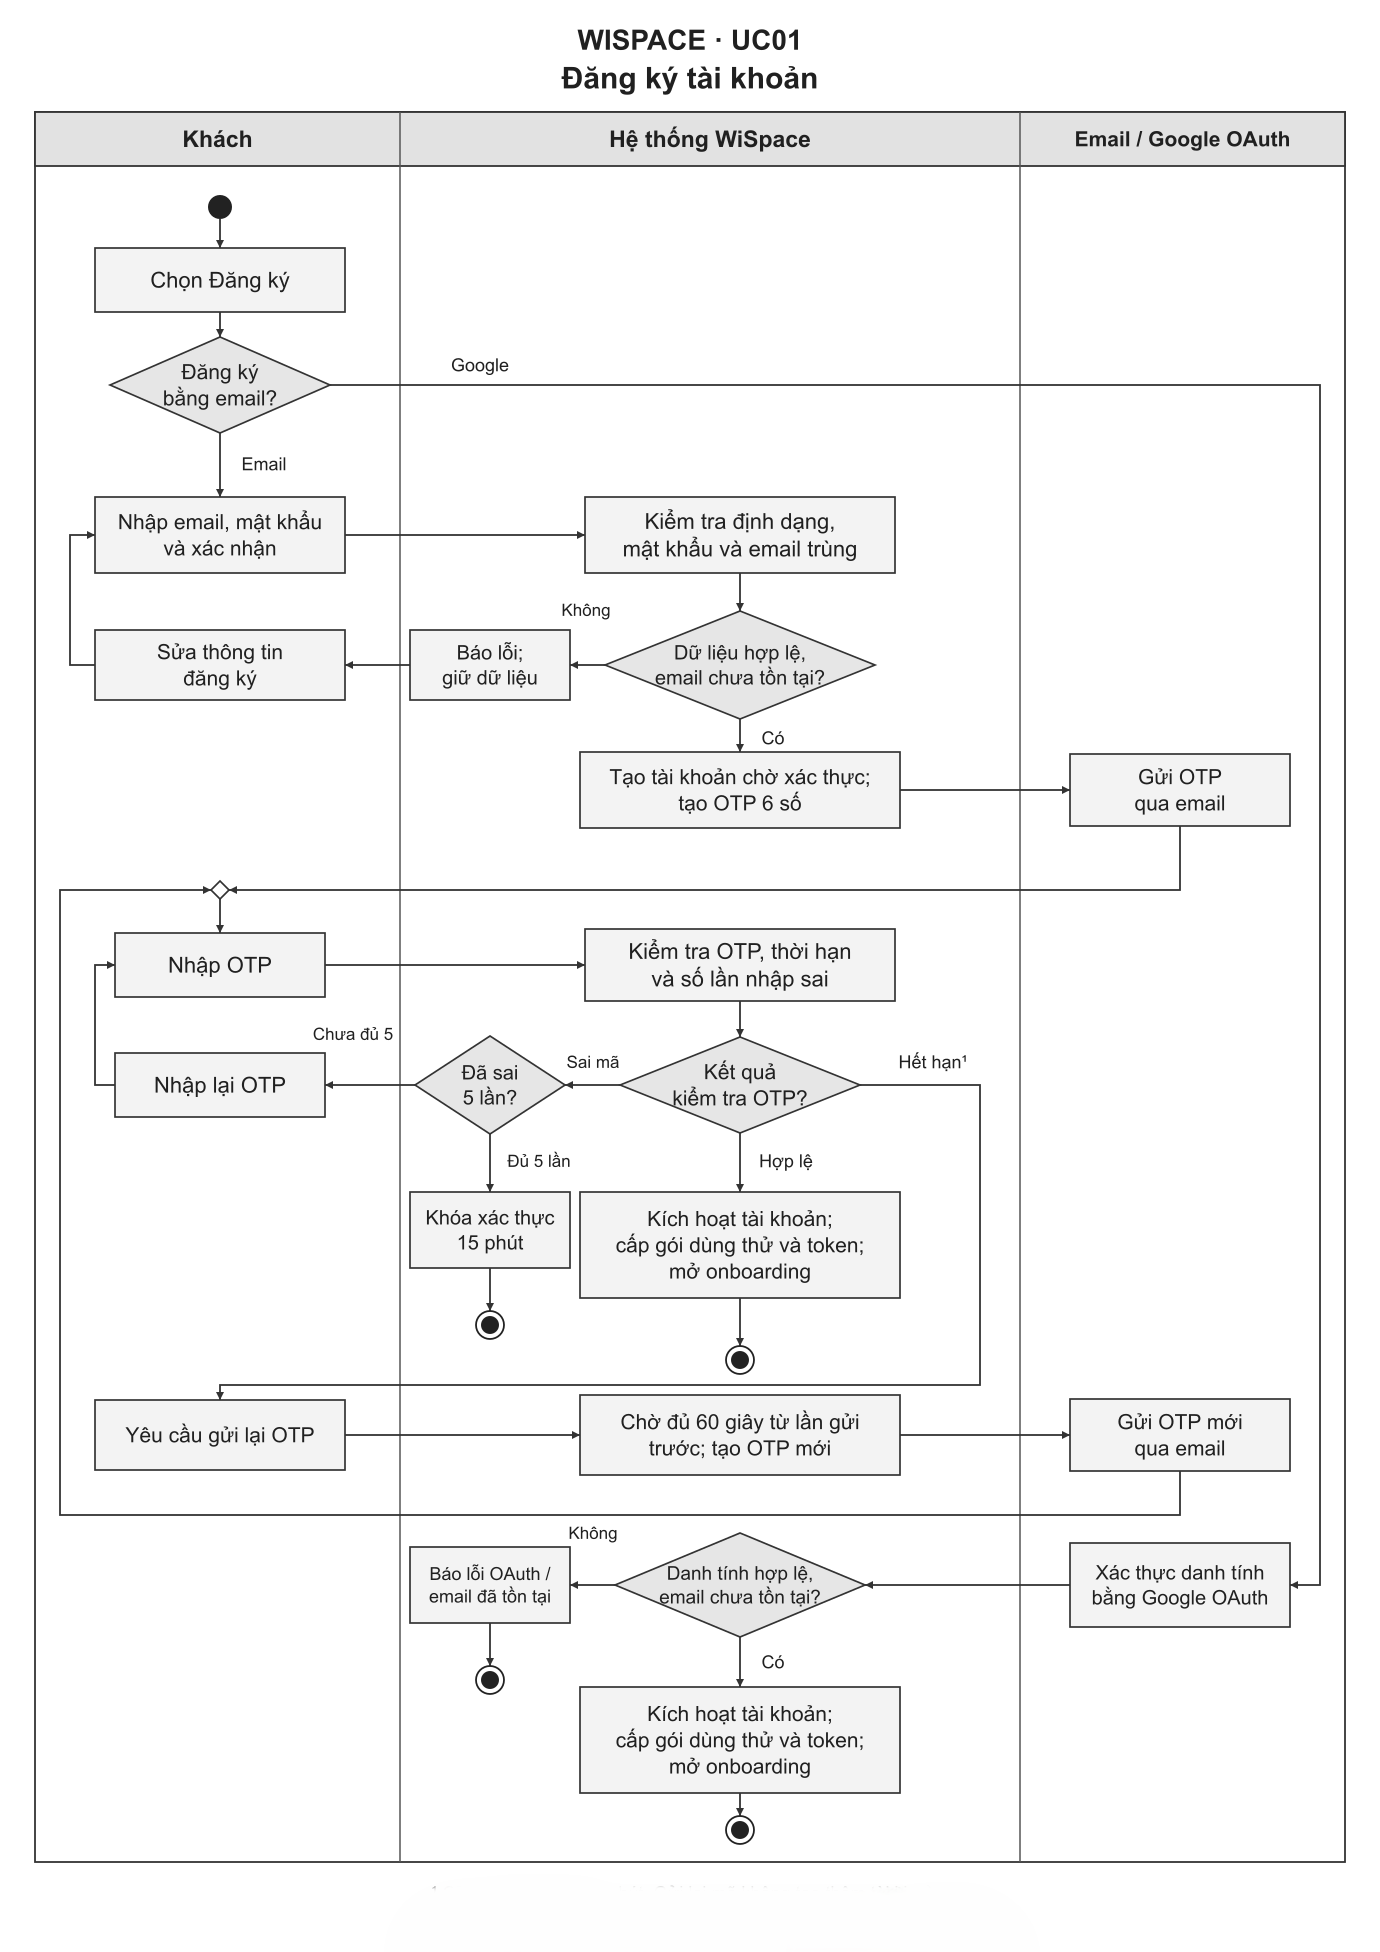
\includegraphics[width=\linewidth,height=0.72\textheight,keepaspectratio]{Images/Activity/Wispace/activity_uc01_register.png}
    \caption{Sơ đồ hoạt động Wispace -- Use-case 1: Đăng ký tài khoản}
    \label{wispace:fig:activity_uc01}
\end{figure}

Khách nhập thông tin đăng ký hoặc chọn Google. Xác thực thành công, hệ thống kích hoạt tài khoản và mở bước thiết lập ban đầu.
% activity-generated:end


\clearpage

\paragraph{Luồng hoạt động: Đăng nhập (Use-case 2)}

% activity-generated:start
\begin{figure}[H]
    \centering
    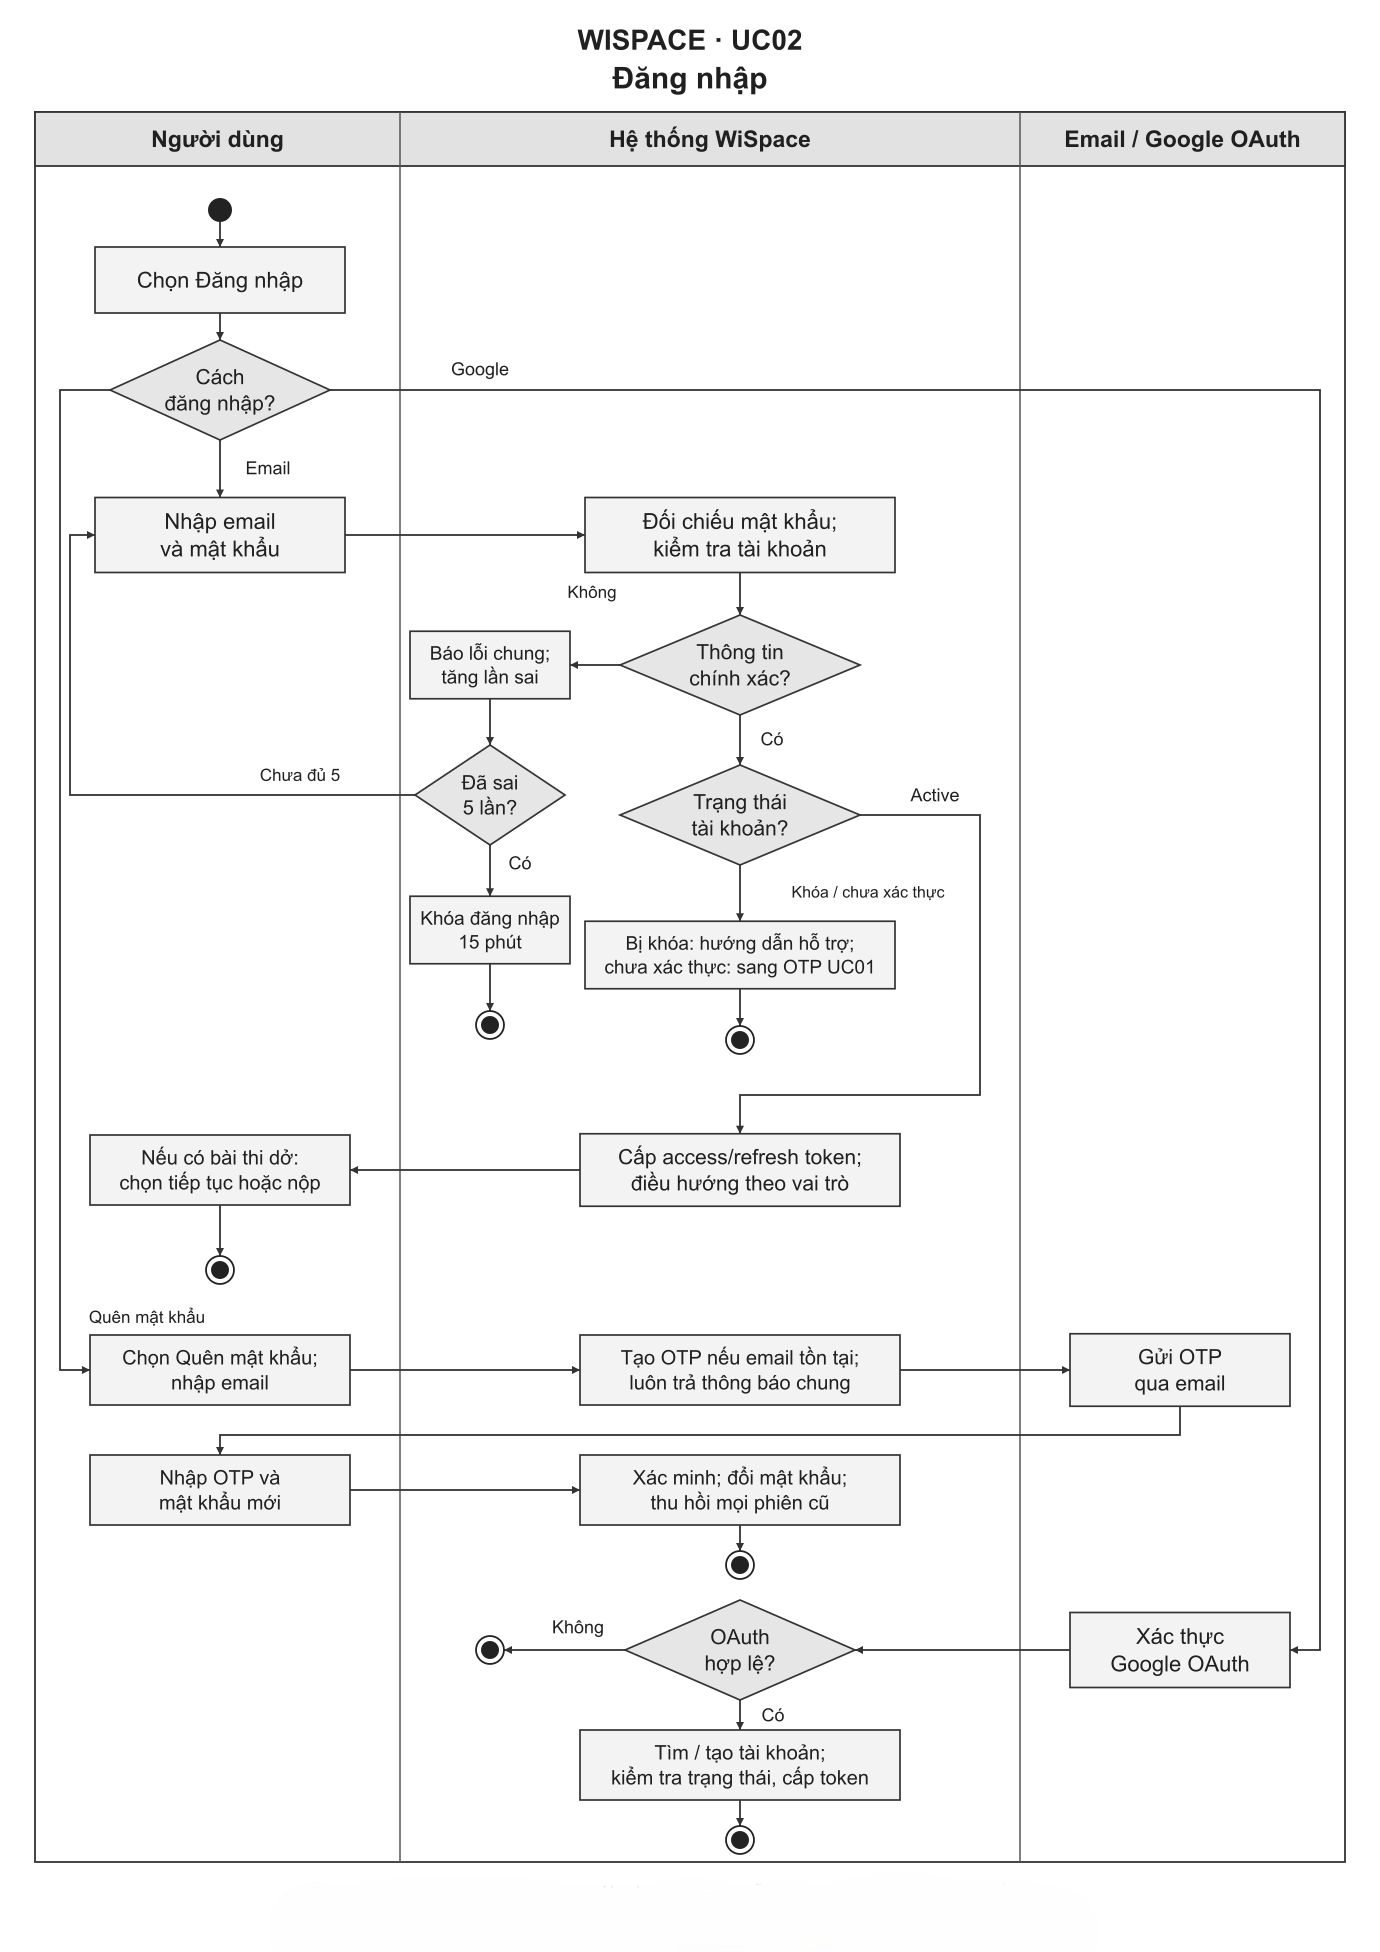
\includegraphics[width=\linewidth,height=0.72\textheight,keepaspectratio]{Images/Activity/Wispace/activity_uc02_login.png}
    \caption{Sơ đồ hoạt động Wispace -- Use-case 2: Đăng nhập}
    \label{wispace:fig:activity_uc02}
\end{figure}

Người dùng nhập thông tin đăng nhập hoặc chọn Google. Đăng nhập thành công, hệ thống chuyển đến giao diện phù hợp với vai trò.
% activity-generated:end


\clearpage

\paragraph{Luồng hoạt động: Đăng xuất (Use-case 3)}

% activity-generated:start
\begin{figure}[H]
    \centering
    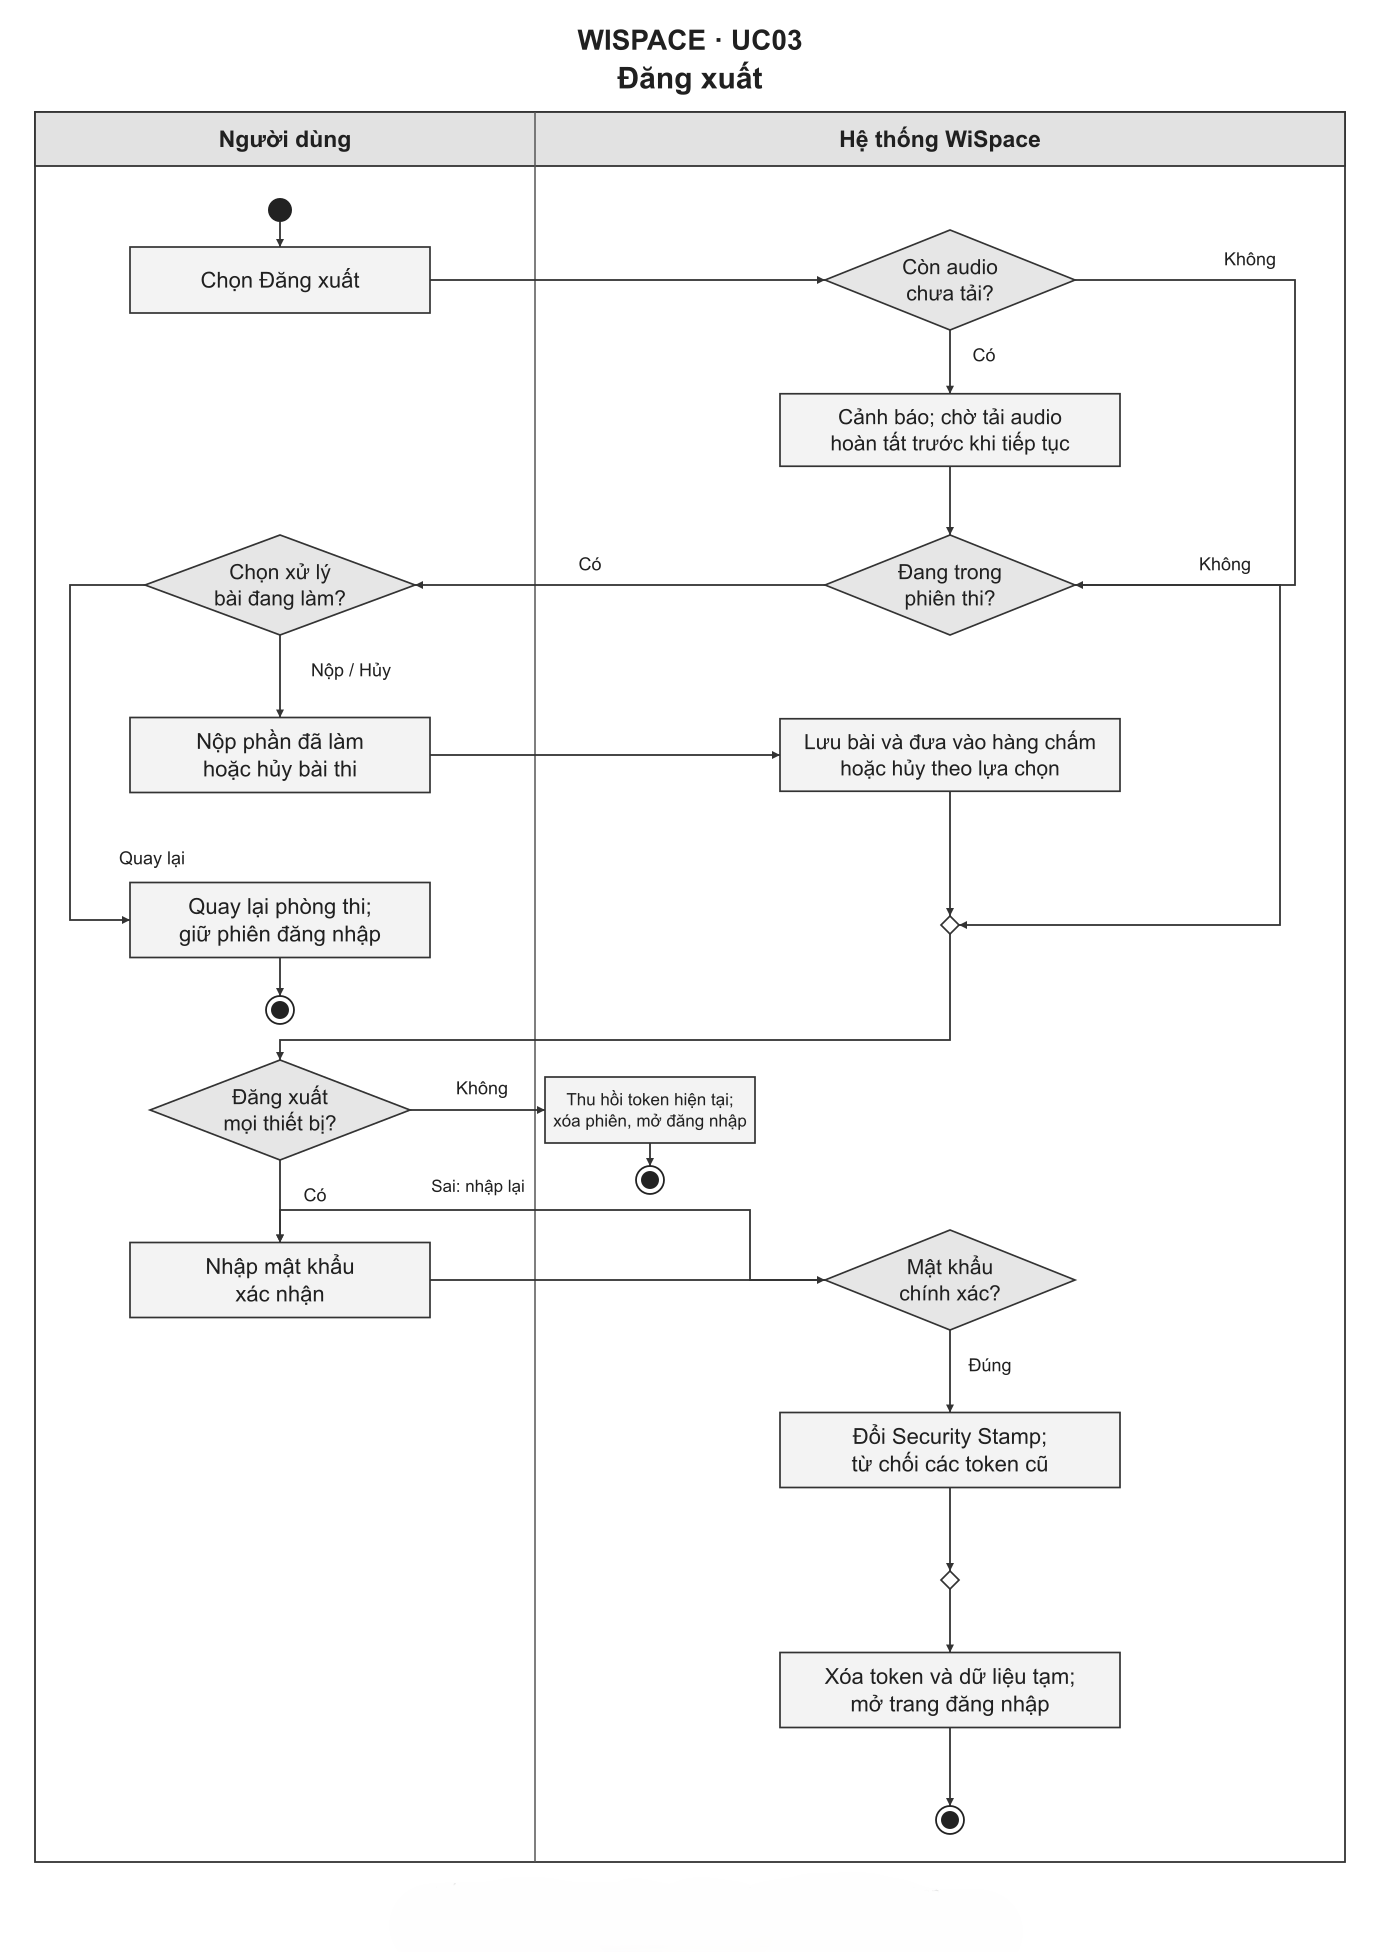
\includegraphics[width=\linewidth,height=0.72\textheight,keepaspectratio]{Images/Activity/Wispace/activity_uc03_logout.png}
    \caption{Sơ đồ hoạt động Wispace -- Use-case 3: Đăng xuất}
    \label{wispace:fig:activity_uc03}
\end{figure}

Người dùng chọn đăng xuất khỏi một hoặc tất cả thiết bị. Giao diện trở về trang đăng nhập.
% activity-generated:end


\clearpage

\paragraph{Luồng hoạt động: Quản lý hồ sơ cá nhân (Use-case 4)}

% activity-generated:start
\begin{figure}[H]
    \centering
    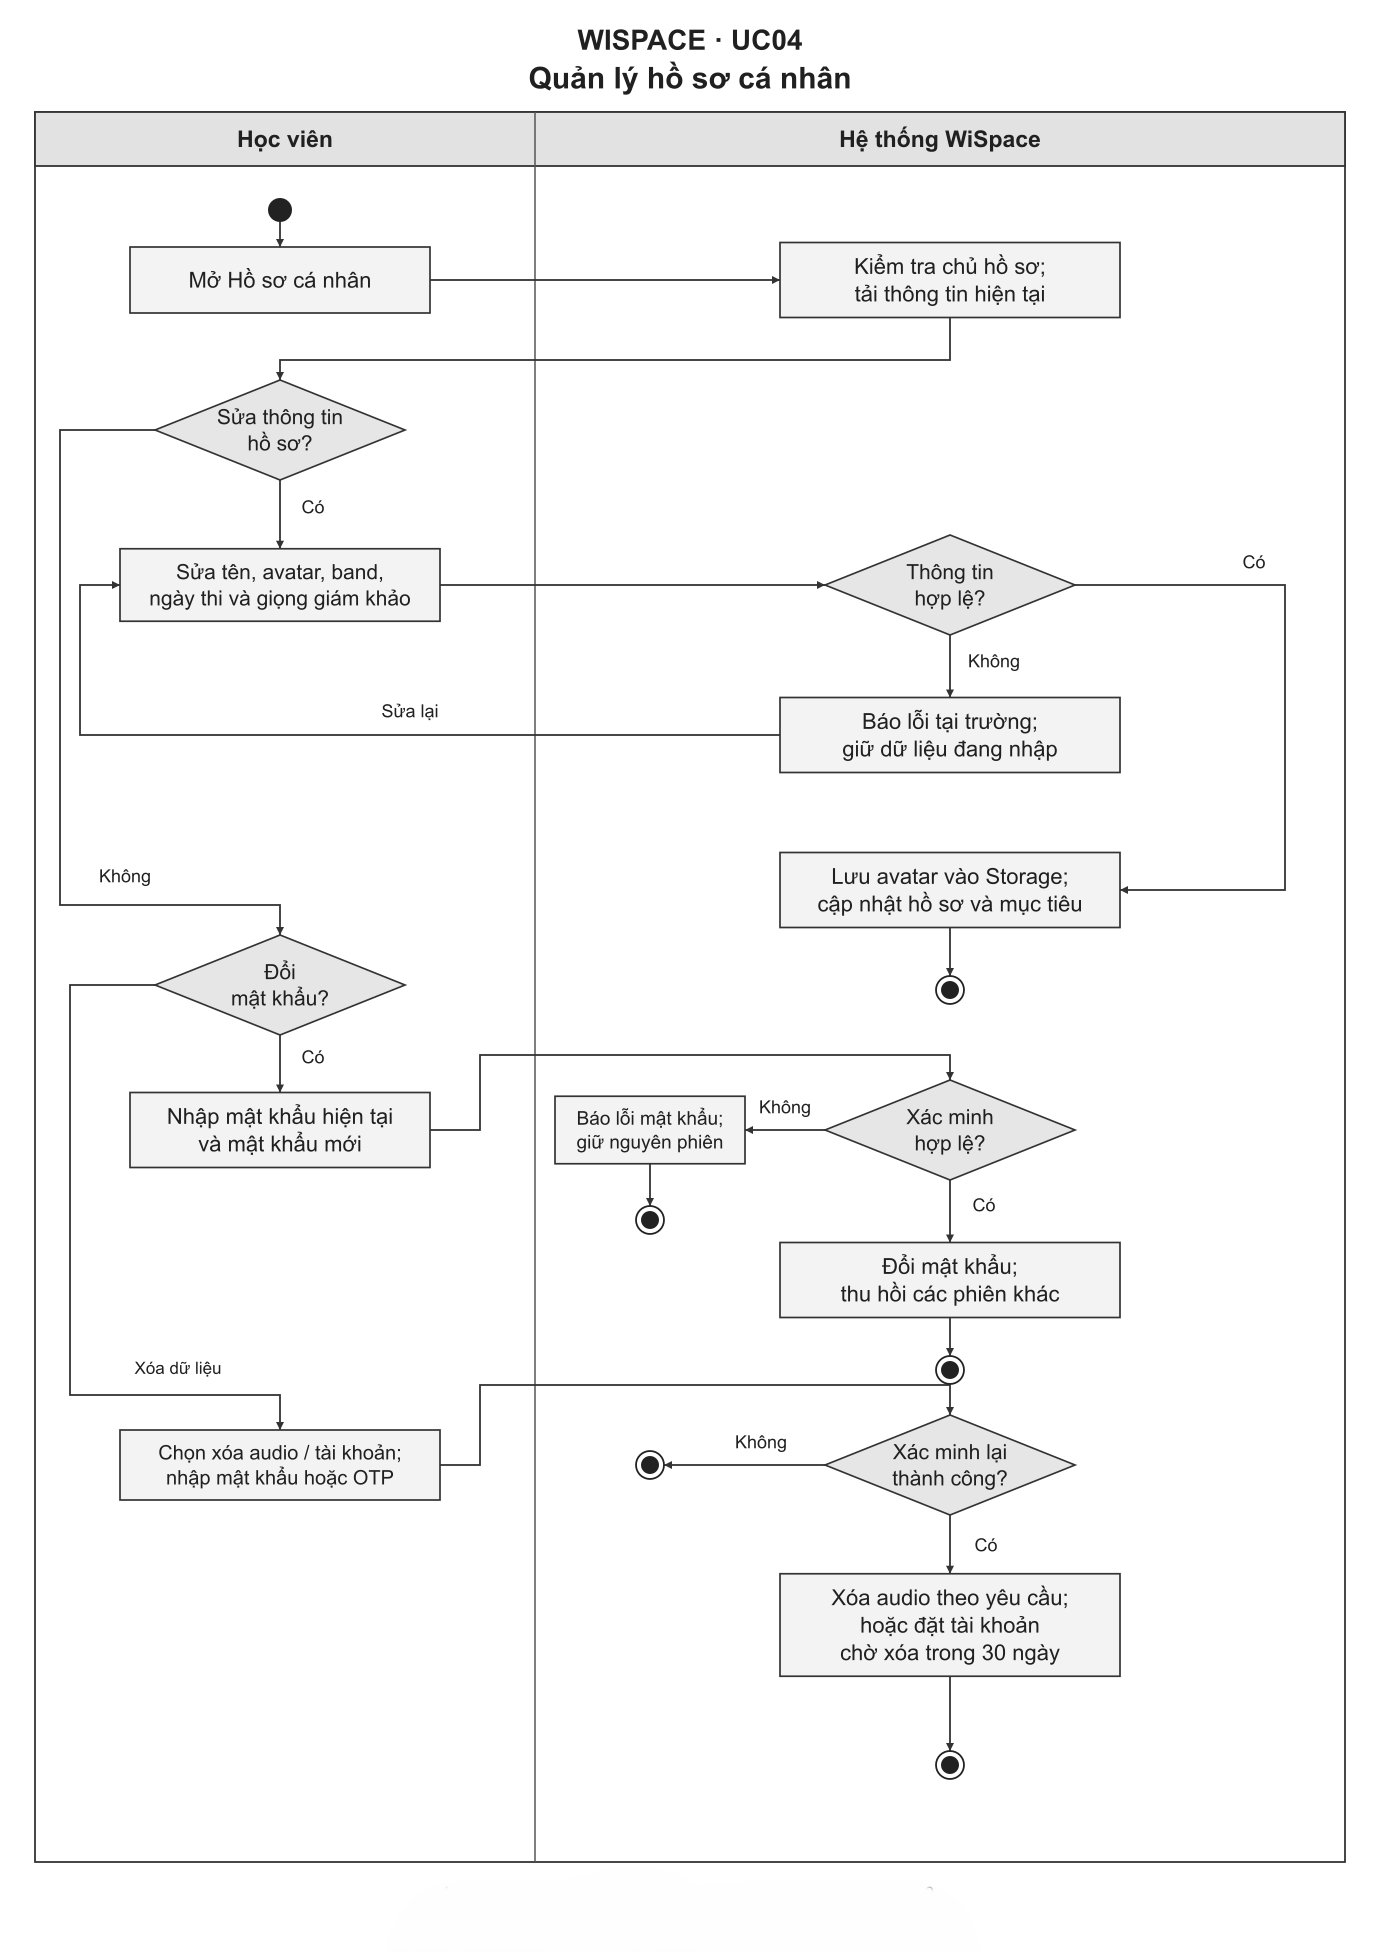
\includegraphics[width=\linewidth,height=0.72\textheight,keepaspectratio]{Images/Activity/Wispace/activity_uc04_profile.png}
    \caption{Sơ đồ hoạt động Wispace -- Use-case 4: Quản lý hồ sơ cá nhân}
    \label{wispace:fig:activity_uc04}
\end{figure}

Học viên mở hồ sơ và chọn nội dung cần thay đổi. Hệ thống xác nhận kết quả cập nhật hoặc xử lý yêu cầu xóa dữ liệu.
% activity-generated:end


\clearpage

\paragraph{Luồng hoạt động: Quản lý người dùng (Use-case 5)}

% activity-generated:start
\begin{figure}[H]
    \centering
    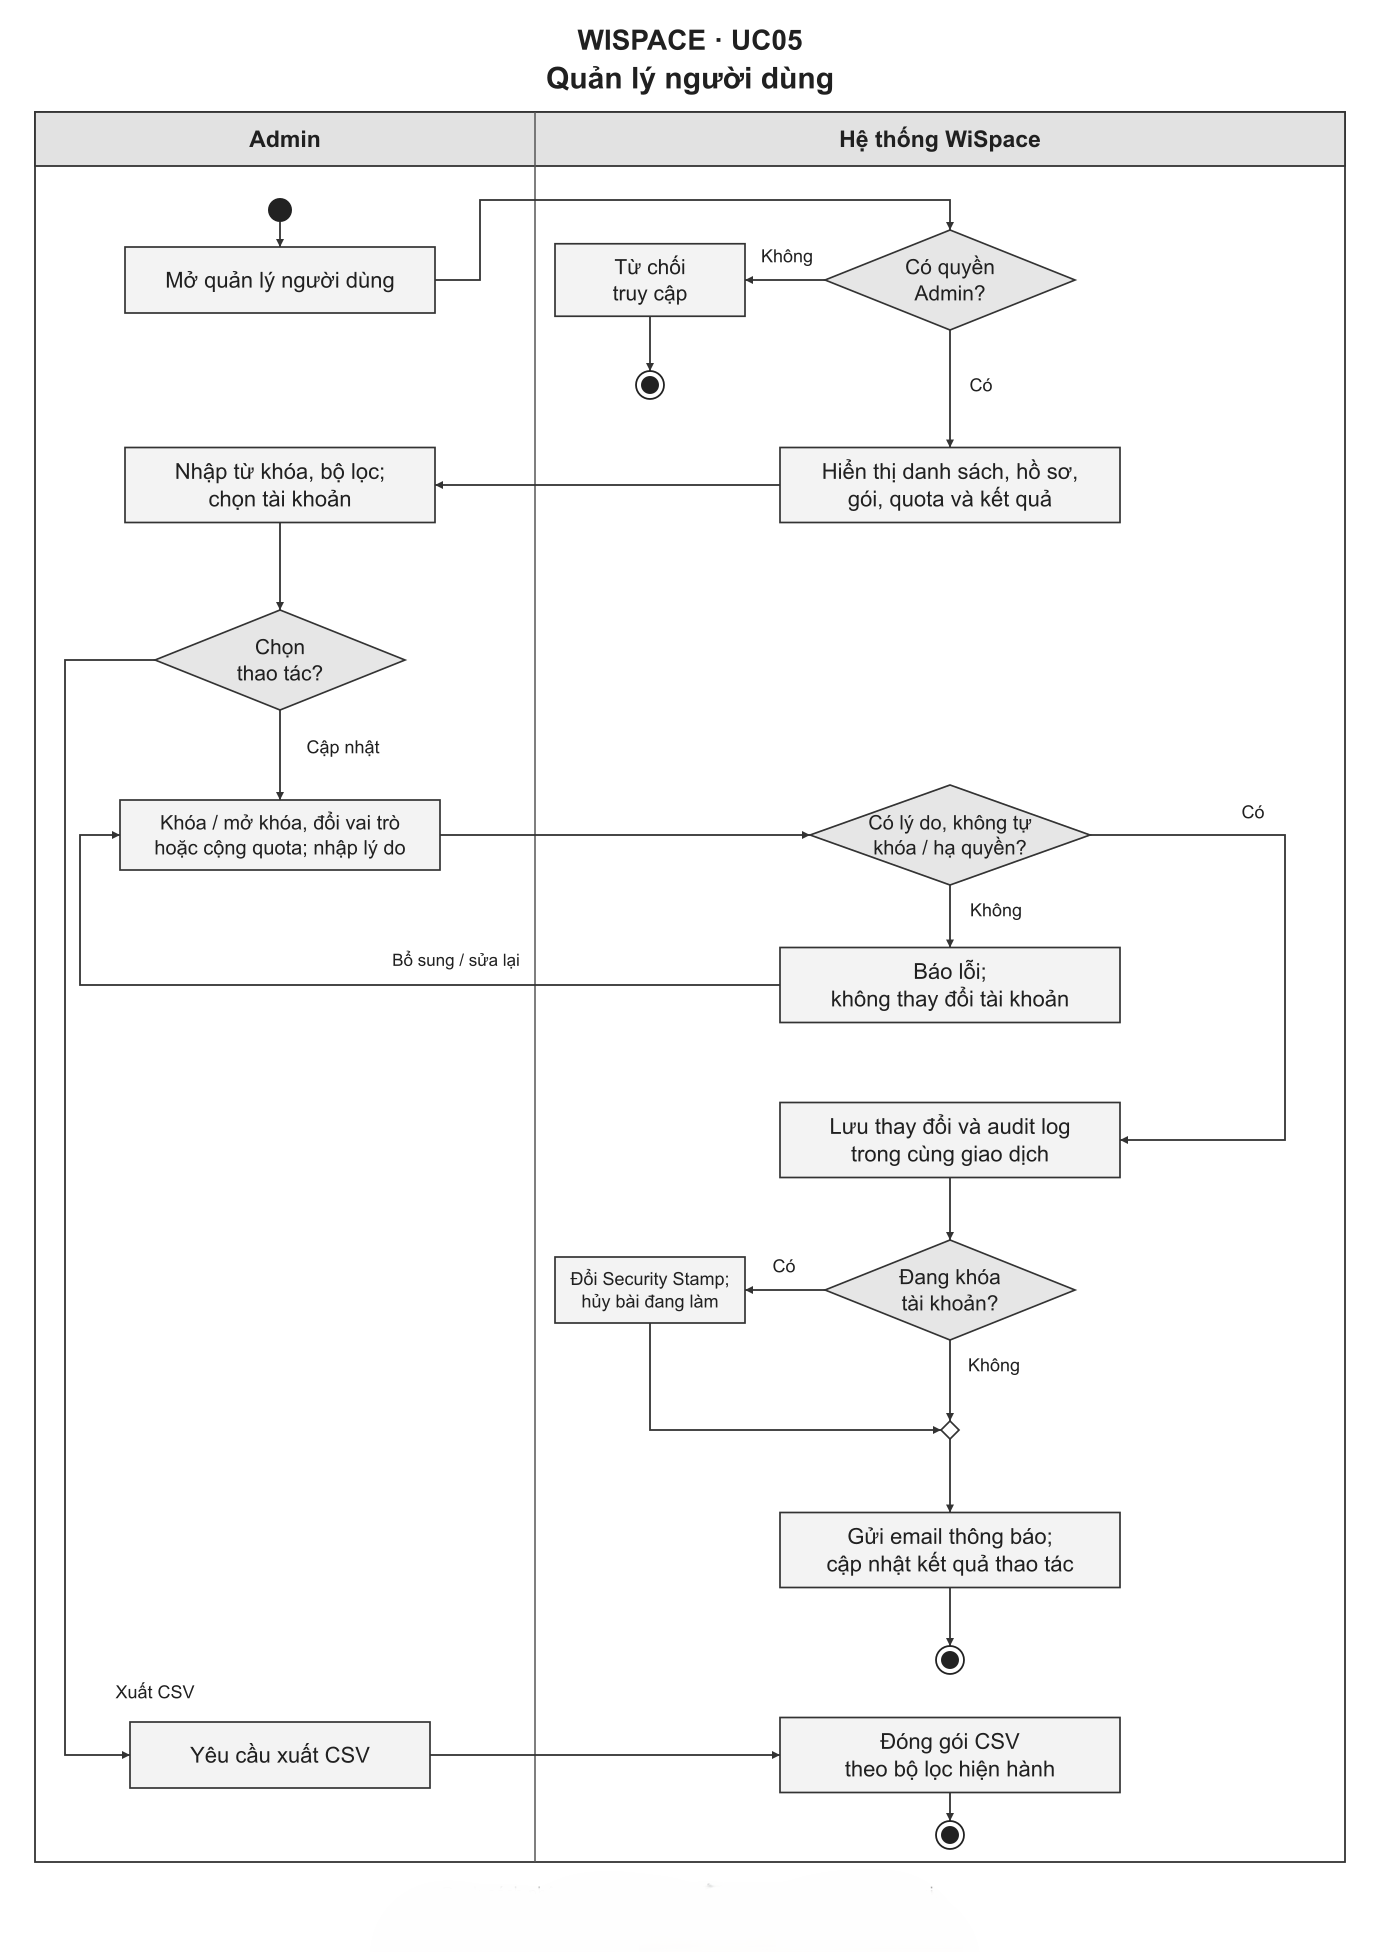
\includegraphics[width=\linewidth,height=0.72\textheight,keepaspectratio]{Images/Activity/Wispace/activity_uc05_user_management.png}
    \caption{Sơ đồ hoạt động Wispace -- Use-case 5: Quản lý người dùng}
    \label{wispace:fig:activity_uc05}
\end{figure}

Admin tìm kiếm và chọn người dùng cần quản lý. Thay đổi được lưu kèm nhật ký; Admin nhận kết quả hoặc xuất danh sách.
% activity-generated:end


\clearpage

\paragraph{Luồng hoạt động: Xem và tìm kiếm đề thi (Use-case 6)}

% activity-generated:start
\begin{figure}[H]
    \centering
    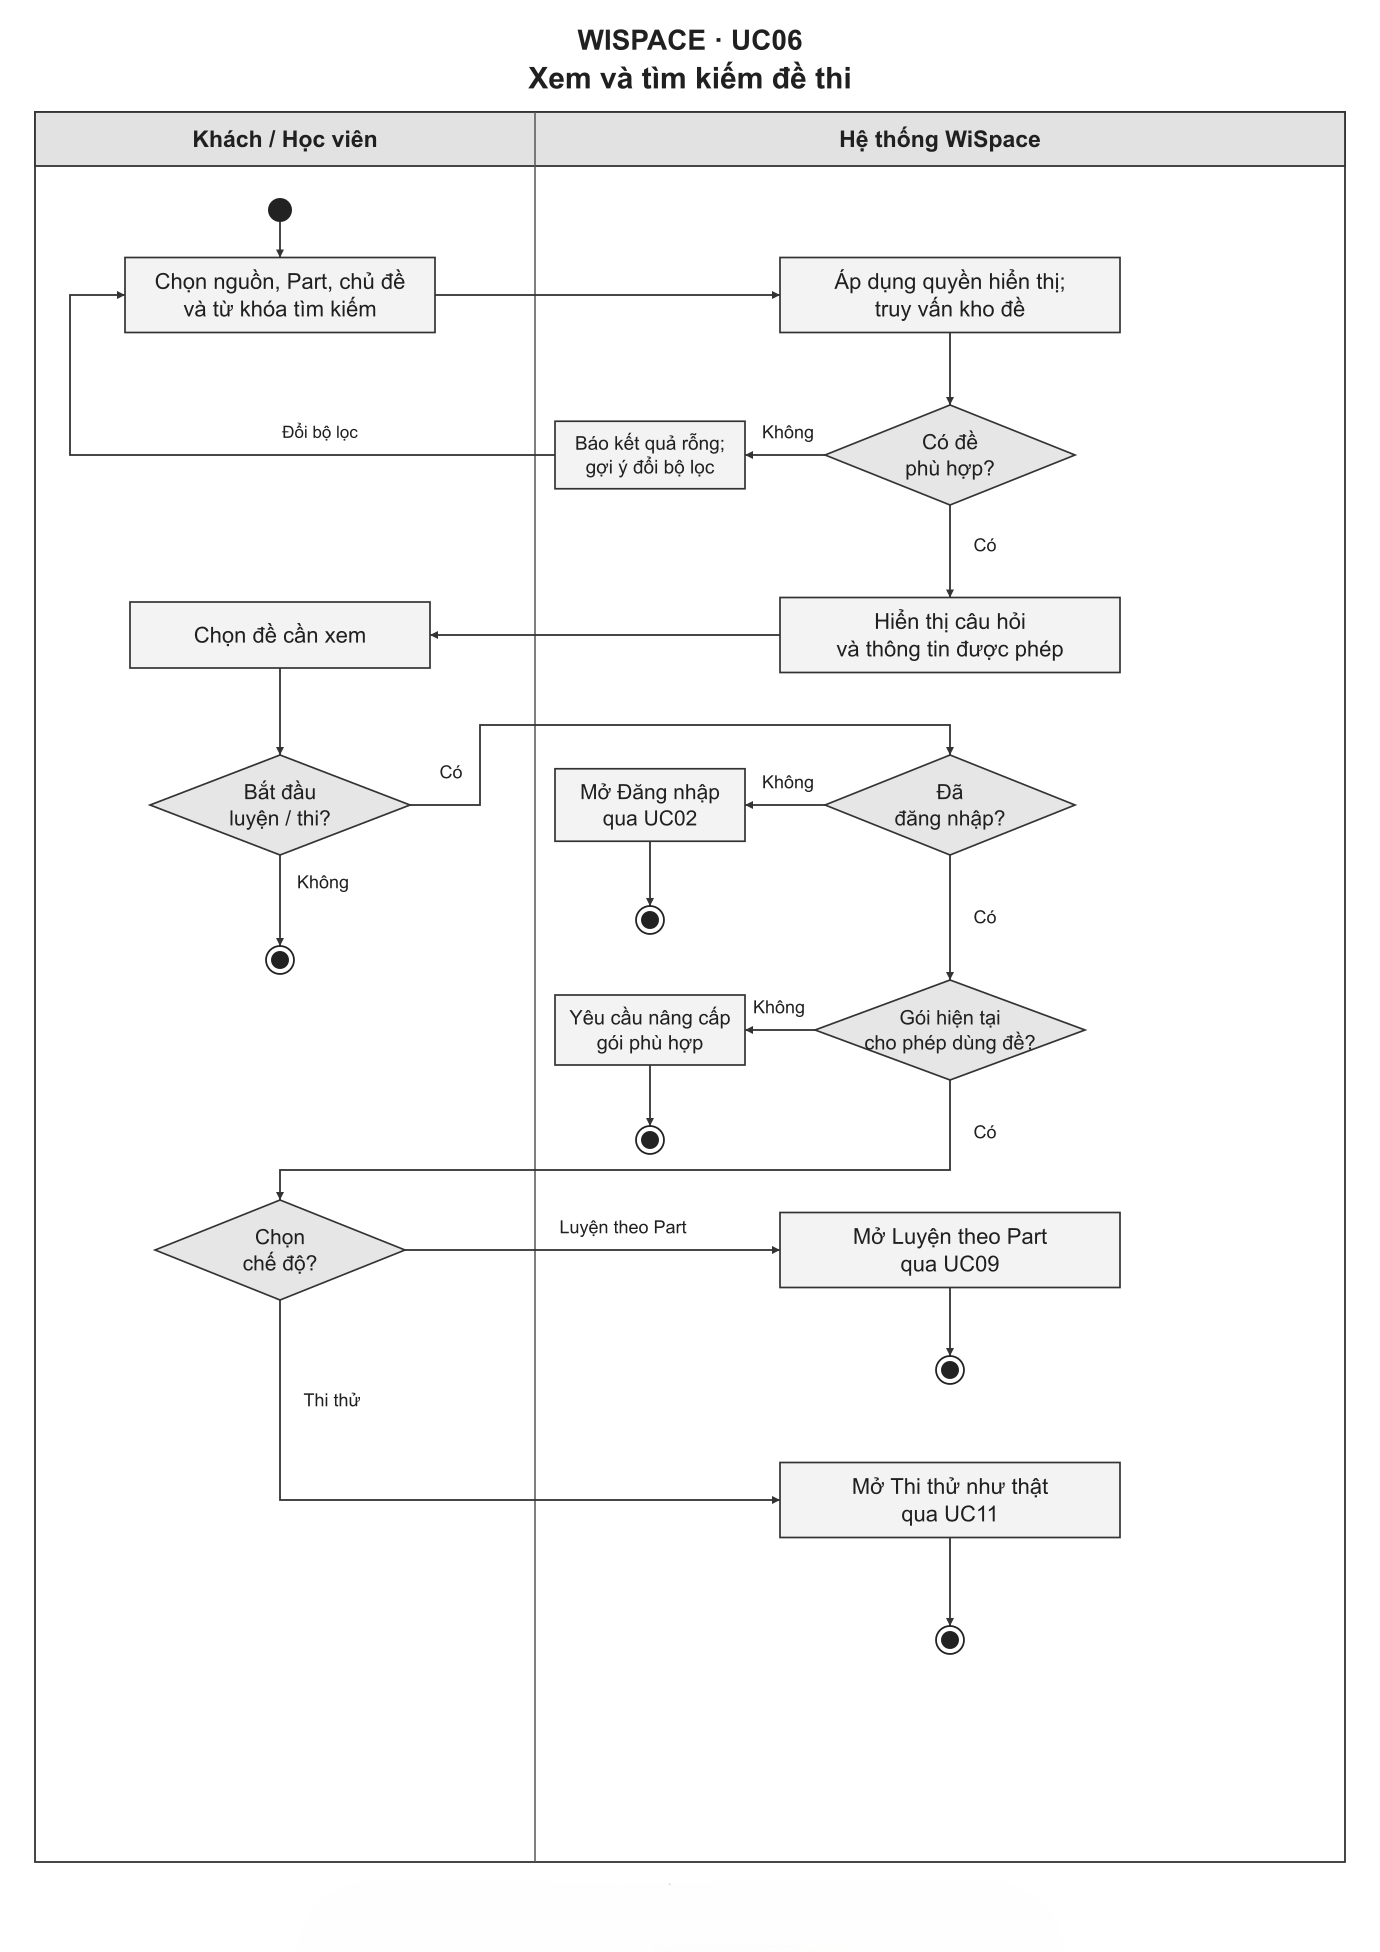
\includegraphics[width=\linewidth,height=0.72\textheight,keepaspectratio]{Images/Activity/Wispace/activity_uc06_browse_tests.png}
    \caption{Sơ đồ hoạt động Wispace -- Use-case 6: Xem và tìm kiếm đề thi}
    \label{wispace:fig:activity_uc06}
\end{figure}

Người dùng chọn nguồn đề, Part, chủ đề hoặc từ khóa. Hệ thống kiểm tra đăng nhập, quyền sử dụng và mở chức năng tương ứng.
% activity-generated:end


\clearpage

\paragraph{Luồng hoạt động: Thêm đề thi (Use-case 7)}

% activity-generated:start
\begin{figure}[H]
    \centering
    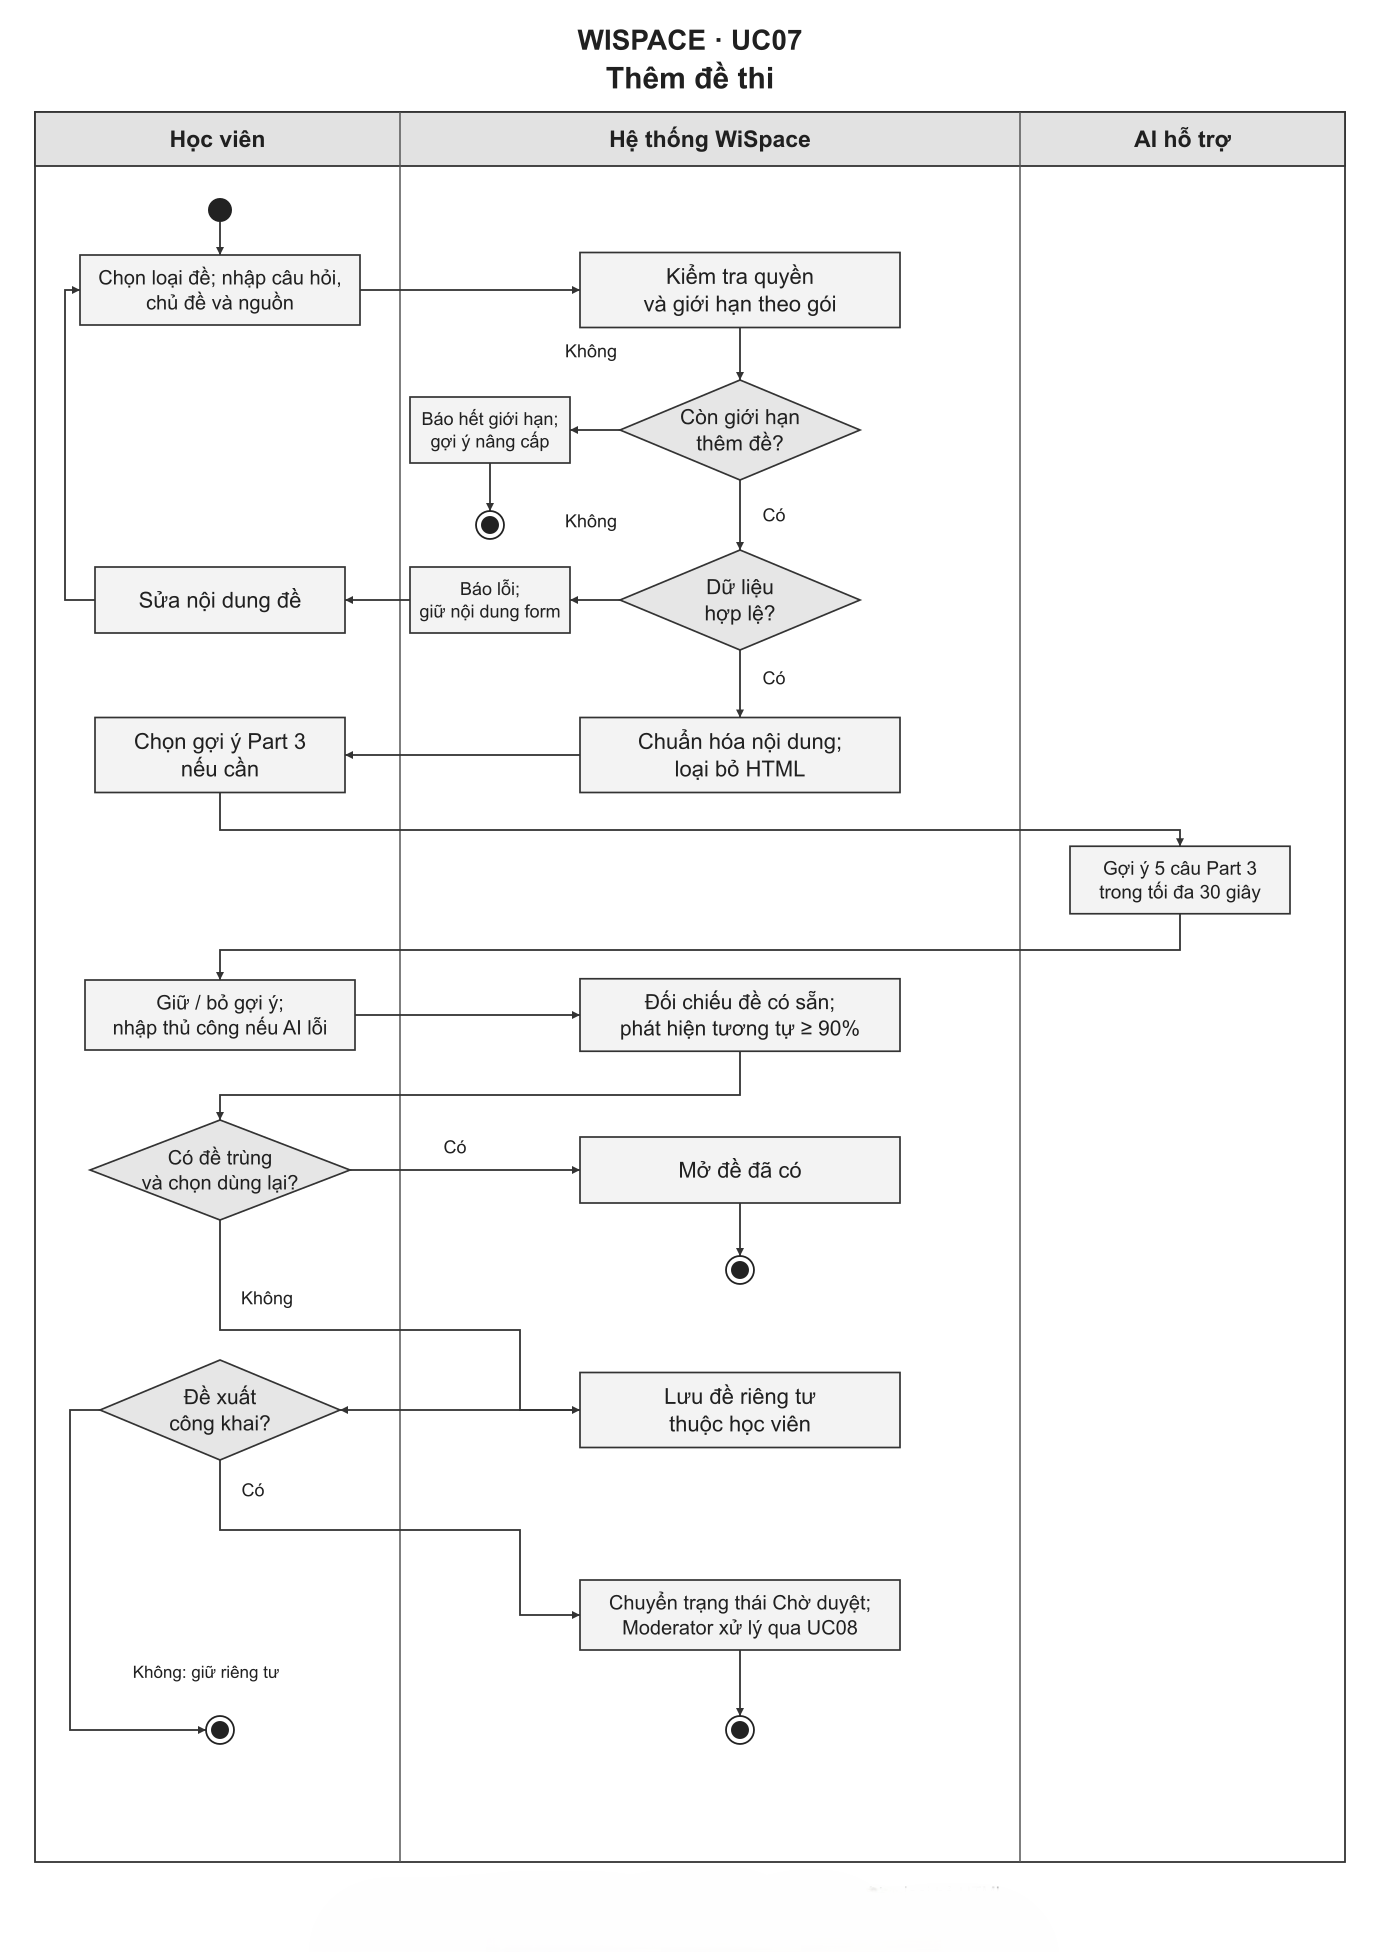
\includegraphics[width=\linewidth,height=0.72\textheight,keepaspectratio]{Images/Activity/Wispace/activity_uc07_add_test.png}
    \caption{Sơ đồ hoạt động Wispace -- Use-case 7: Thêm đề thi}
    \label{wispace:fig:activity_uc07}
\end{figure}

Học viên nhập câu hỏi và thông tin đề cần tạo. Nếu đề xuất công khai, đề được chuyển sang hàng chờ kiểm duyệt.
% activity-generated:end


\clearpage

\paragraph{Luồng hoạt động: Quản lý và duyệt kho đề (Use-case 8)}

% activity-generated:start
\begin{figure}[H]
    \centering
    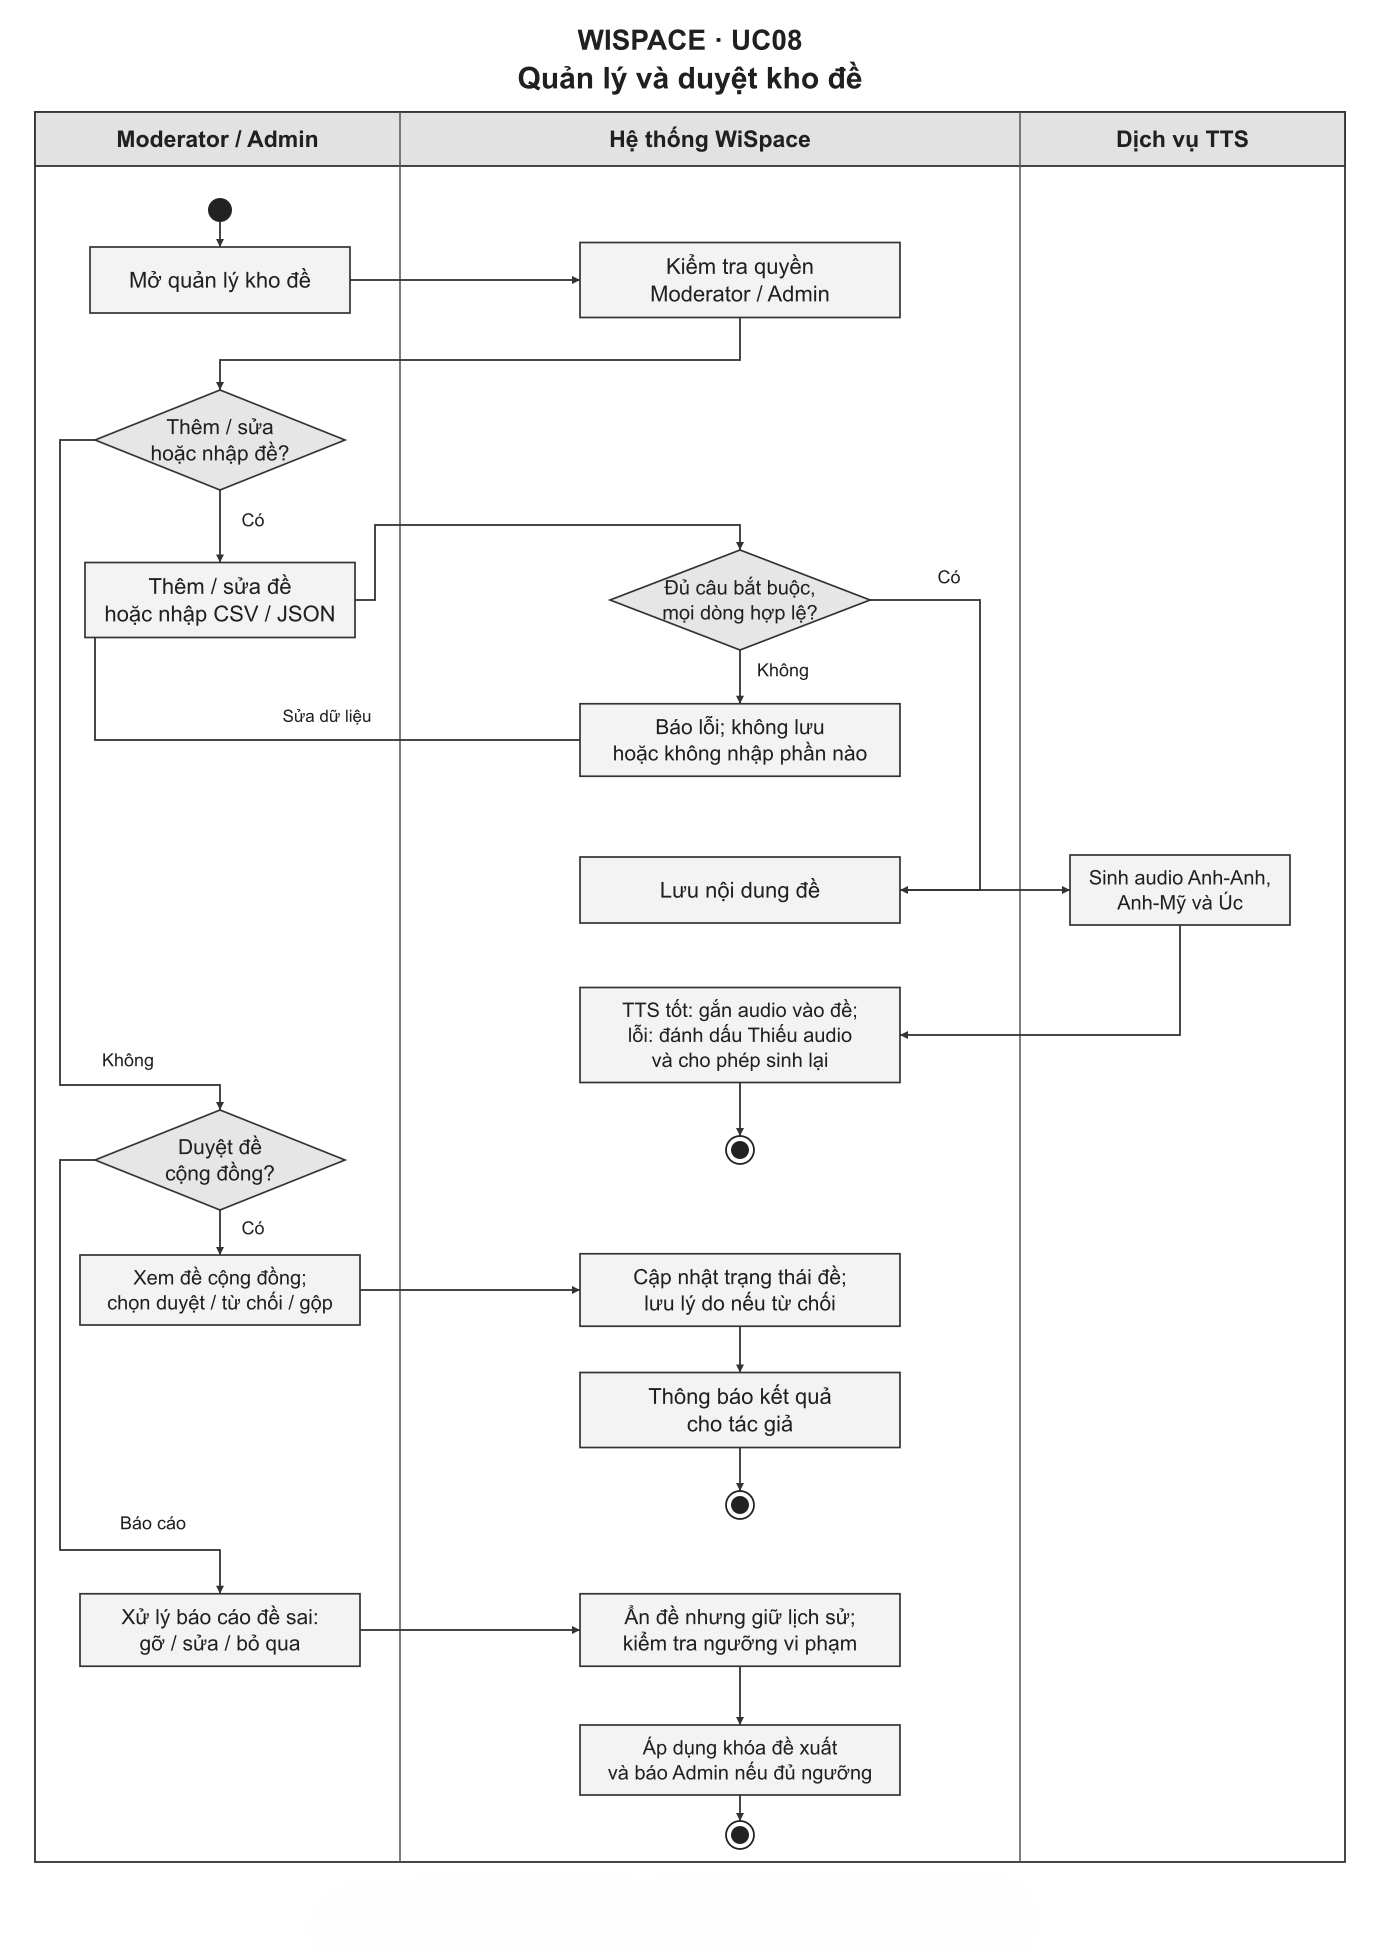
\includegraphics[width=\linewidth,height=0.72\textheight,keepaspectratio]{Images/Activity/Wispace/activity_uc08_moderate_tests.png}
    \caption{Sơ đồ hoạt động Wispace -- Use-case 8: Quản lý và duyệt kho đề}
    \label{wispace:fig:activity_uc08}
\end{figure}

Moderator hoặc Admin chọn thêm, sửa, nhập đề hoặc duyệt đề cộng đồng. Các báo cáo đề sai được xử lý mà vẫn giữ lịch sử bài làm.
% activity-generated:end


\clearpage

\paragraph{Luồng hoạt động: Luyện tập theo Part (Use-case 9)}

% activity-generated:start
\begin{figure}[H]
    \centering
    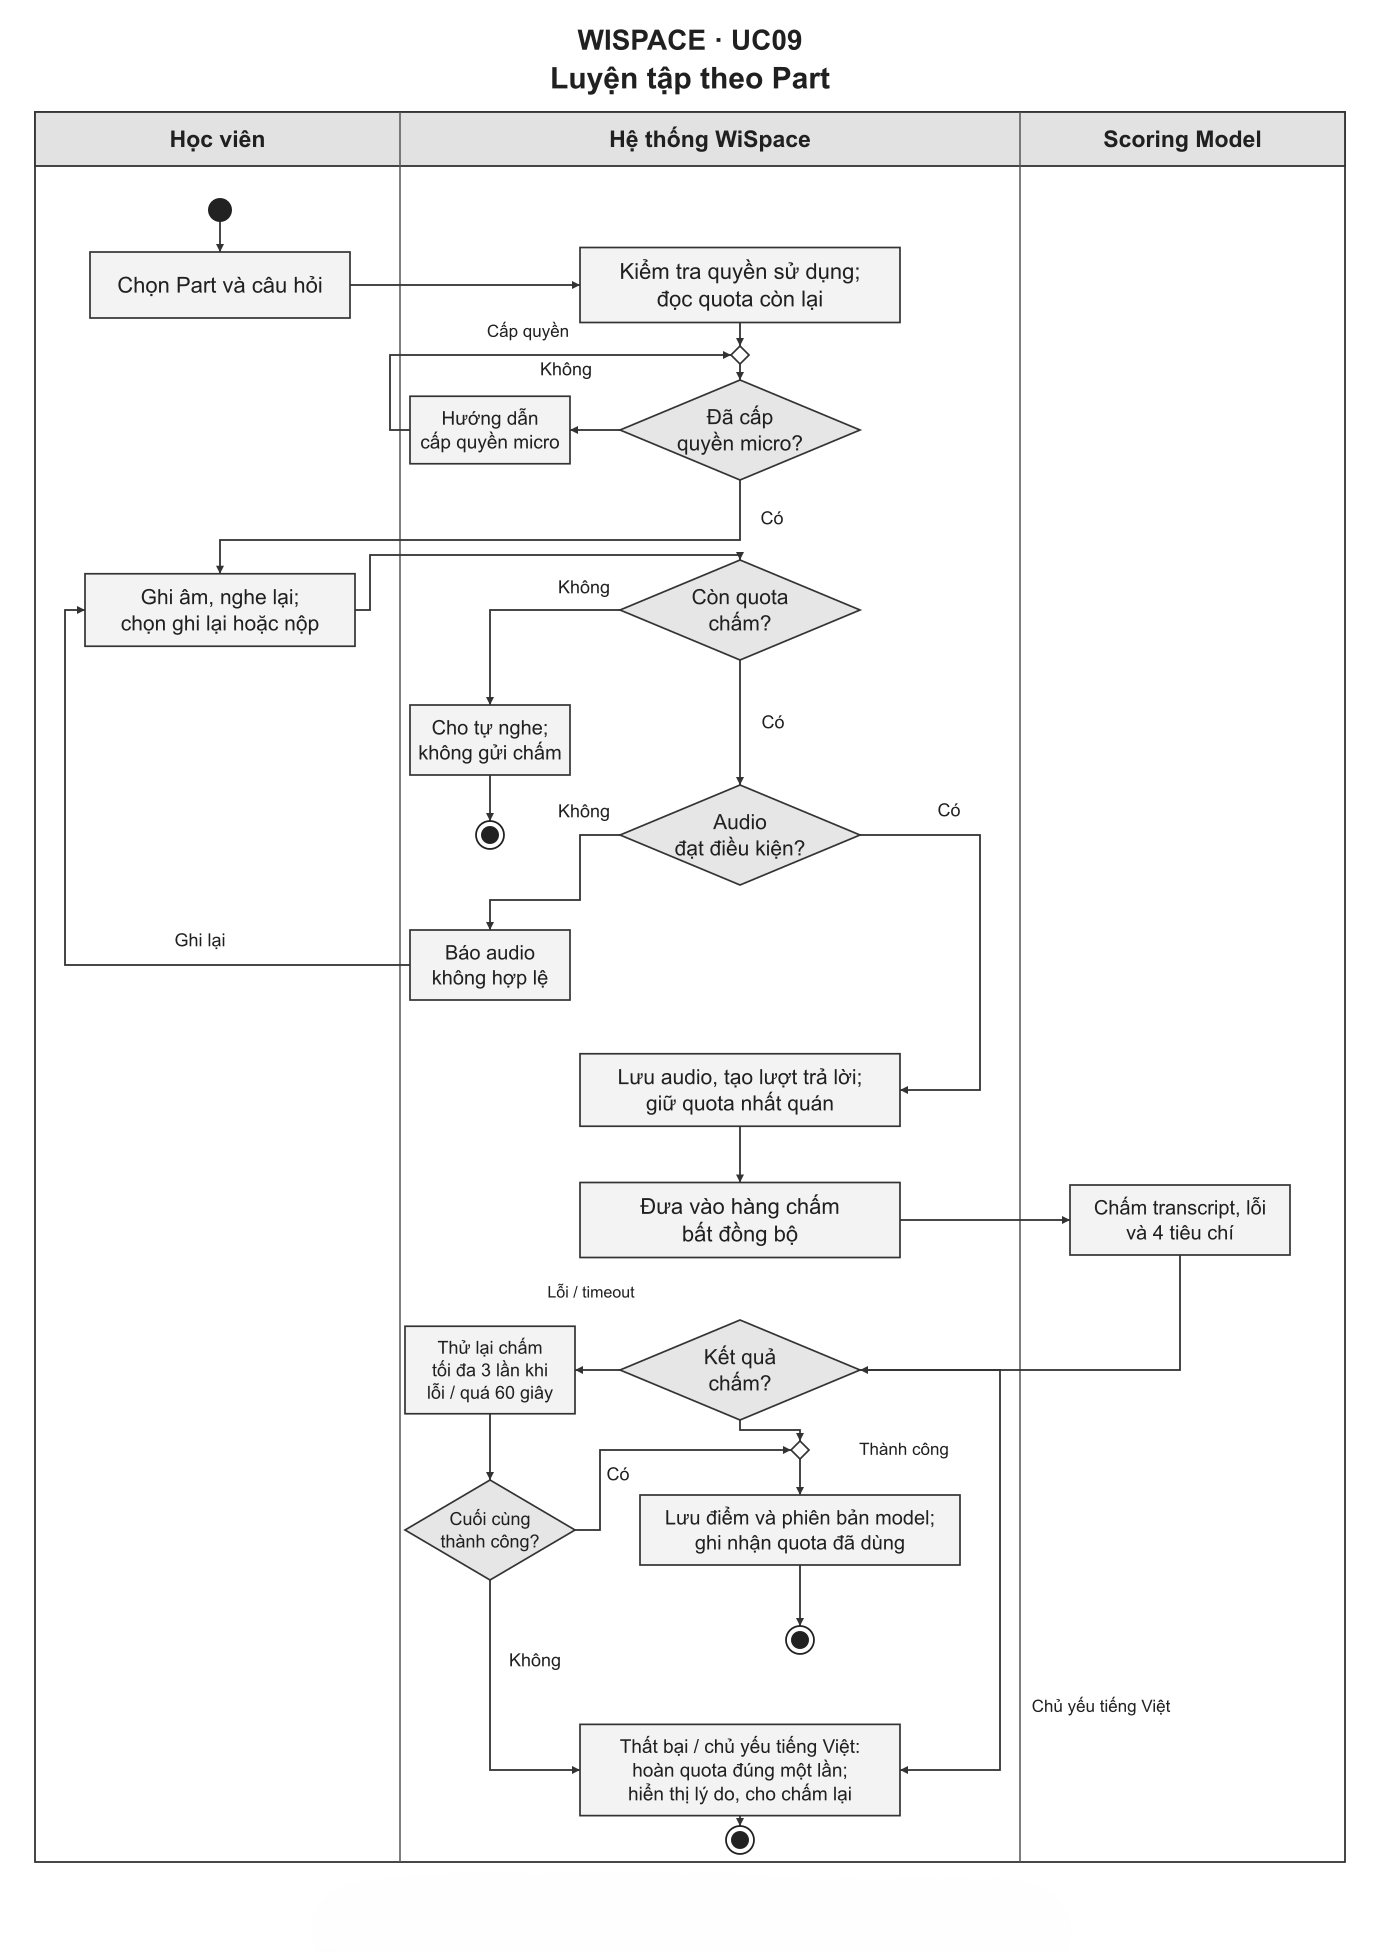
\includegraphics[width=\linewidth,height=0.72\textheight,keepaspectratio]{Images/Activity/Wispace/activity_uc09_part_practice.png}
    \caption{Sơ đồ hoạt động Wispace -- Use-case 9: Luyện tập theo Part}
    \label{wispace:fig:activity_uc09}
\end{figure}

Học viên chọn câu hỏi, ghi âm và nộp câu trả lời. Hệ thống lưu kết quả; nếu chấm thất bại cuối cùng thì hoàn hạn mức.
% activity-generated:end


\clearpage

\paragraph{Luồng hoạt động: Xem kết quả và luyện lại (Use-case 10)}

% activity-generated:start
\begin{figure}[H]
    \centering
    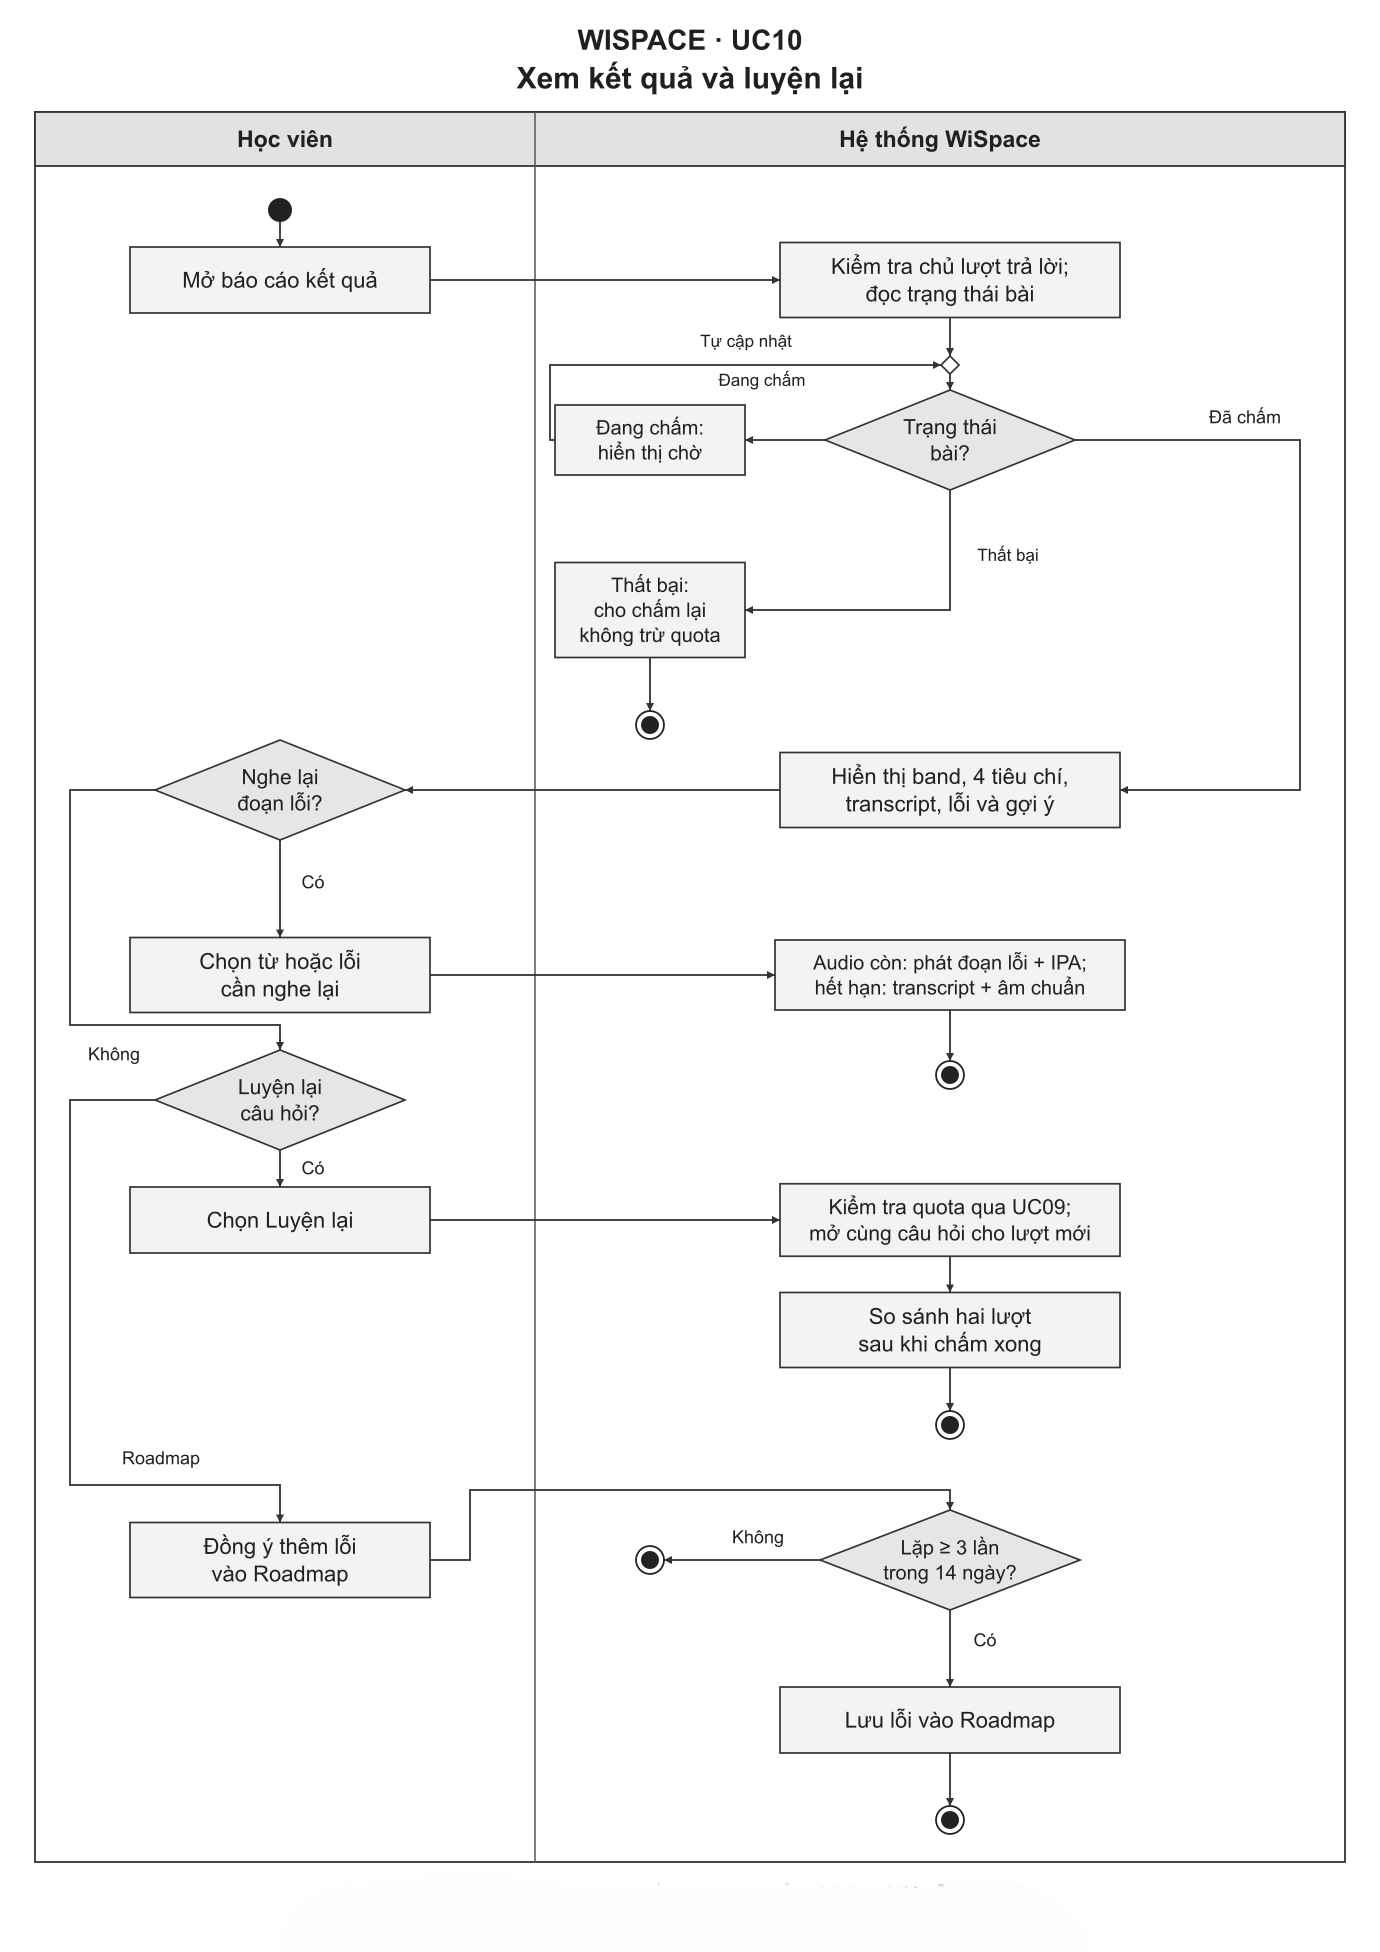
\includegraphics[width=\linewidth,height=0.72\textheight,keepaspectratio]{Images/Activity/Wispace/activity_uc10_results_retry.png}
    \caption{Sơ đồ hoạt động Wispace -- Use-case 10: Xem kết quả và luyện lại}
    \label{wispace:fig:activity_uc10}
\end{figure}

Học viên mở kết quả của bài đã nộp. Hệ thống thực hiện lựa chọn và lưu kết quả liên quan.
% activity-generated:end


\clearpage

\paragraph{Luồng hoạt động: Thi thử như thật (Use-case 11)}

% activity-generated:start
\begin{figure}[H]
    \centering
    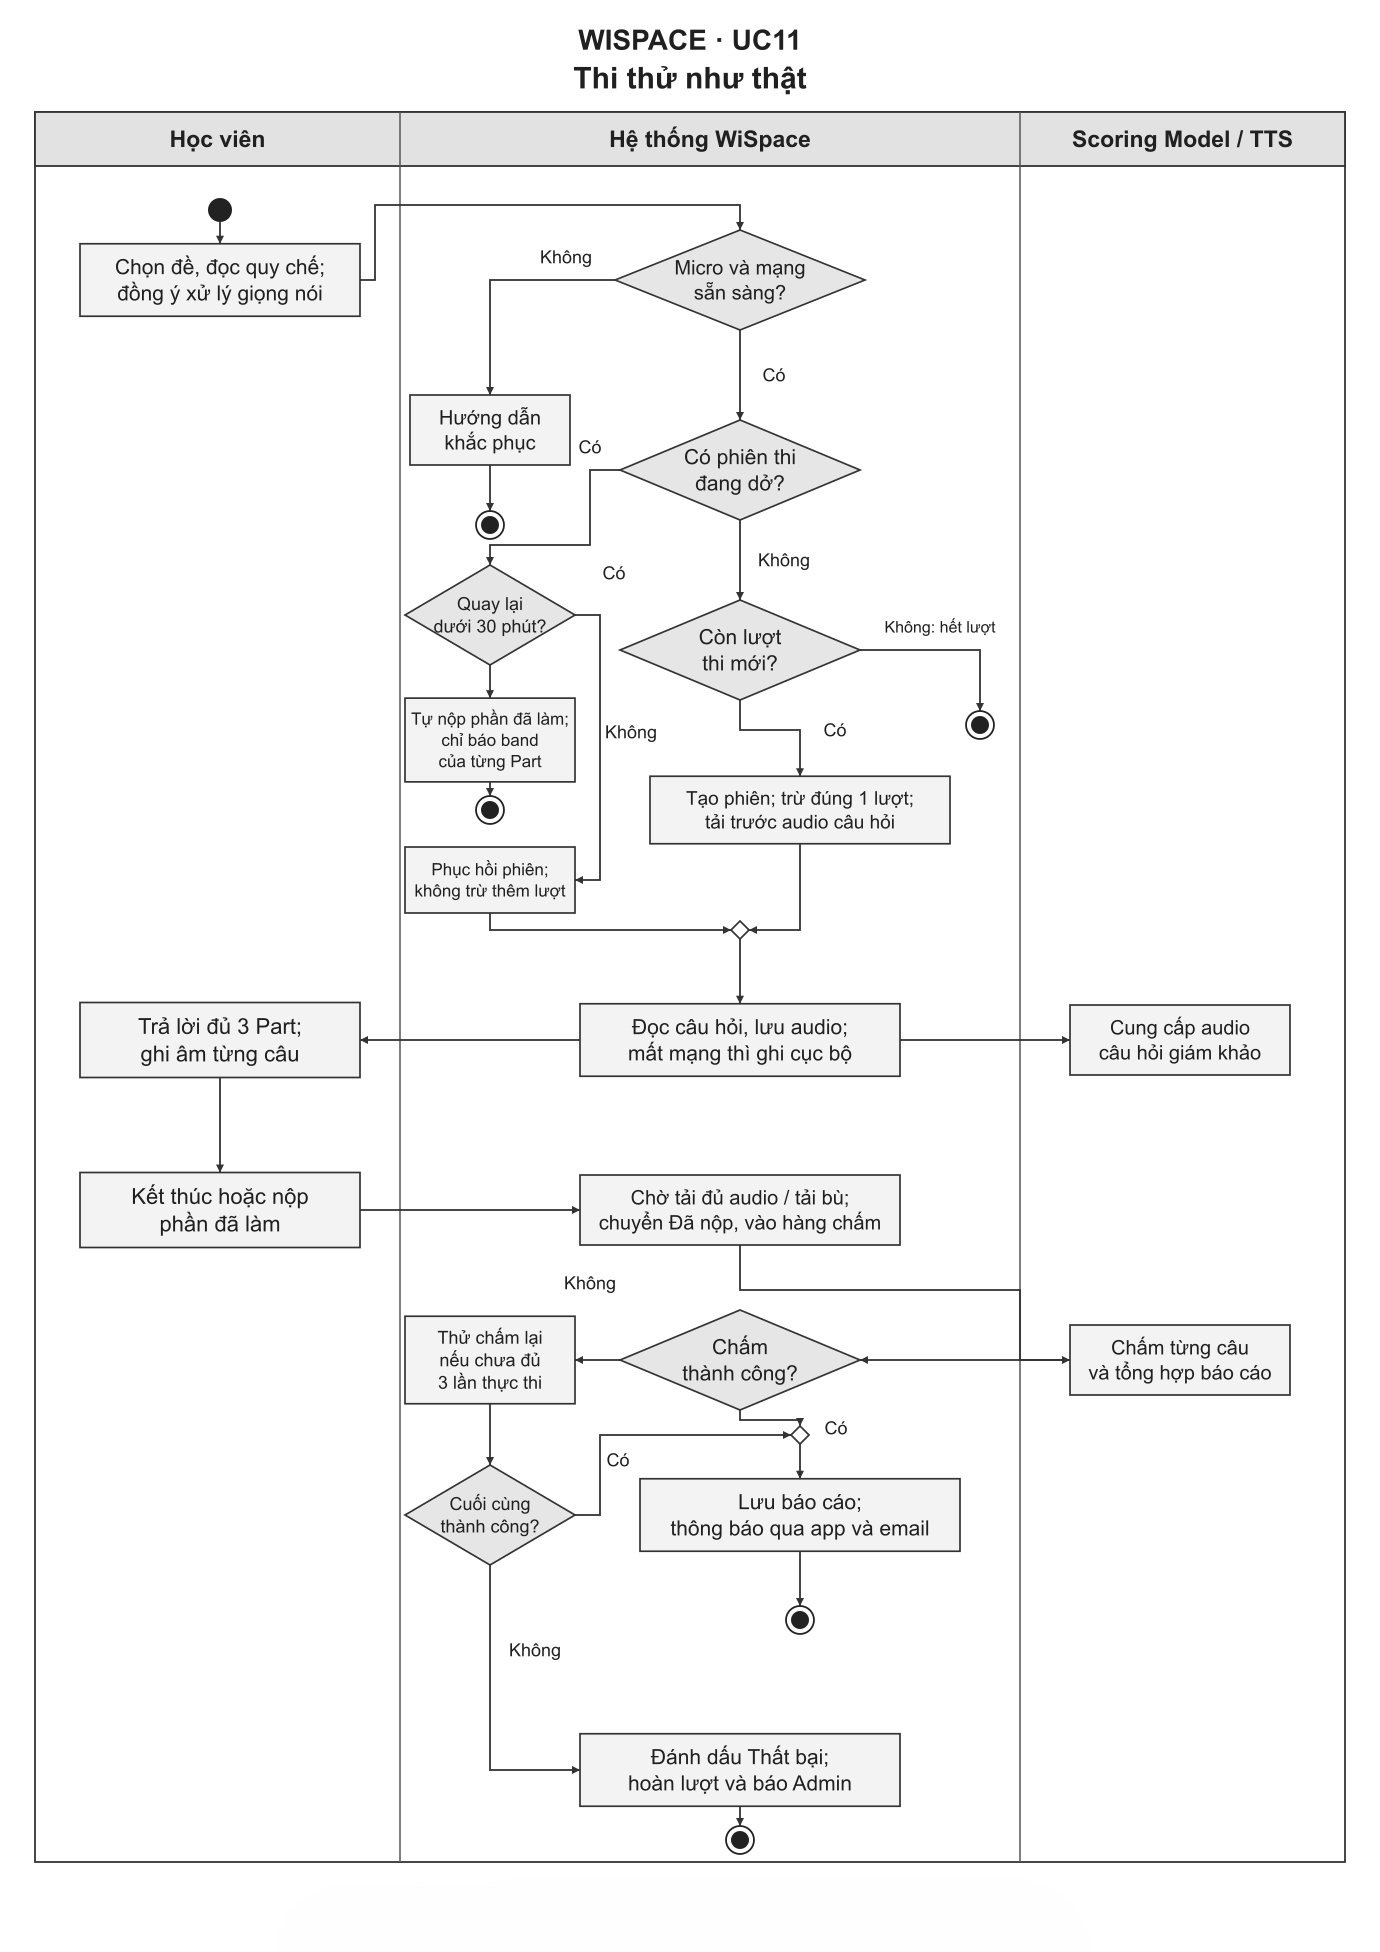
\includegraphics[width=\linewidth,height=0.72\textheight,keepaspectratio]{Images/Activity/Wispace/activity_uc11_mock_test.png}
    \caption{Sơ đồ hoạt động Wispace -- Use-case 11: Thi thử như thật}
    \label{wispace:fig:activity_uc11}
\end{figure}

Học viên chọn đề, kiểm tra thiết bị và bắt đầu hoặc tiếp tục phiên thi. Báo cáo được lưu và thông báo; nếu chấm thất bại cuối cùng thì hoàn lượt.
% activity-generated:end


\clearpage

\paragraph{Luồng hoạt động: Xem lịch sử và tiến bộ (Use-case 12)}

% activity-generated:start
\begin{figure}[H]
    \centering
    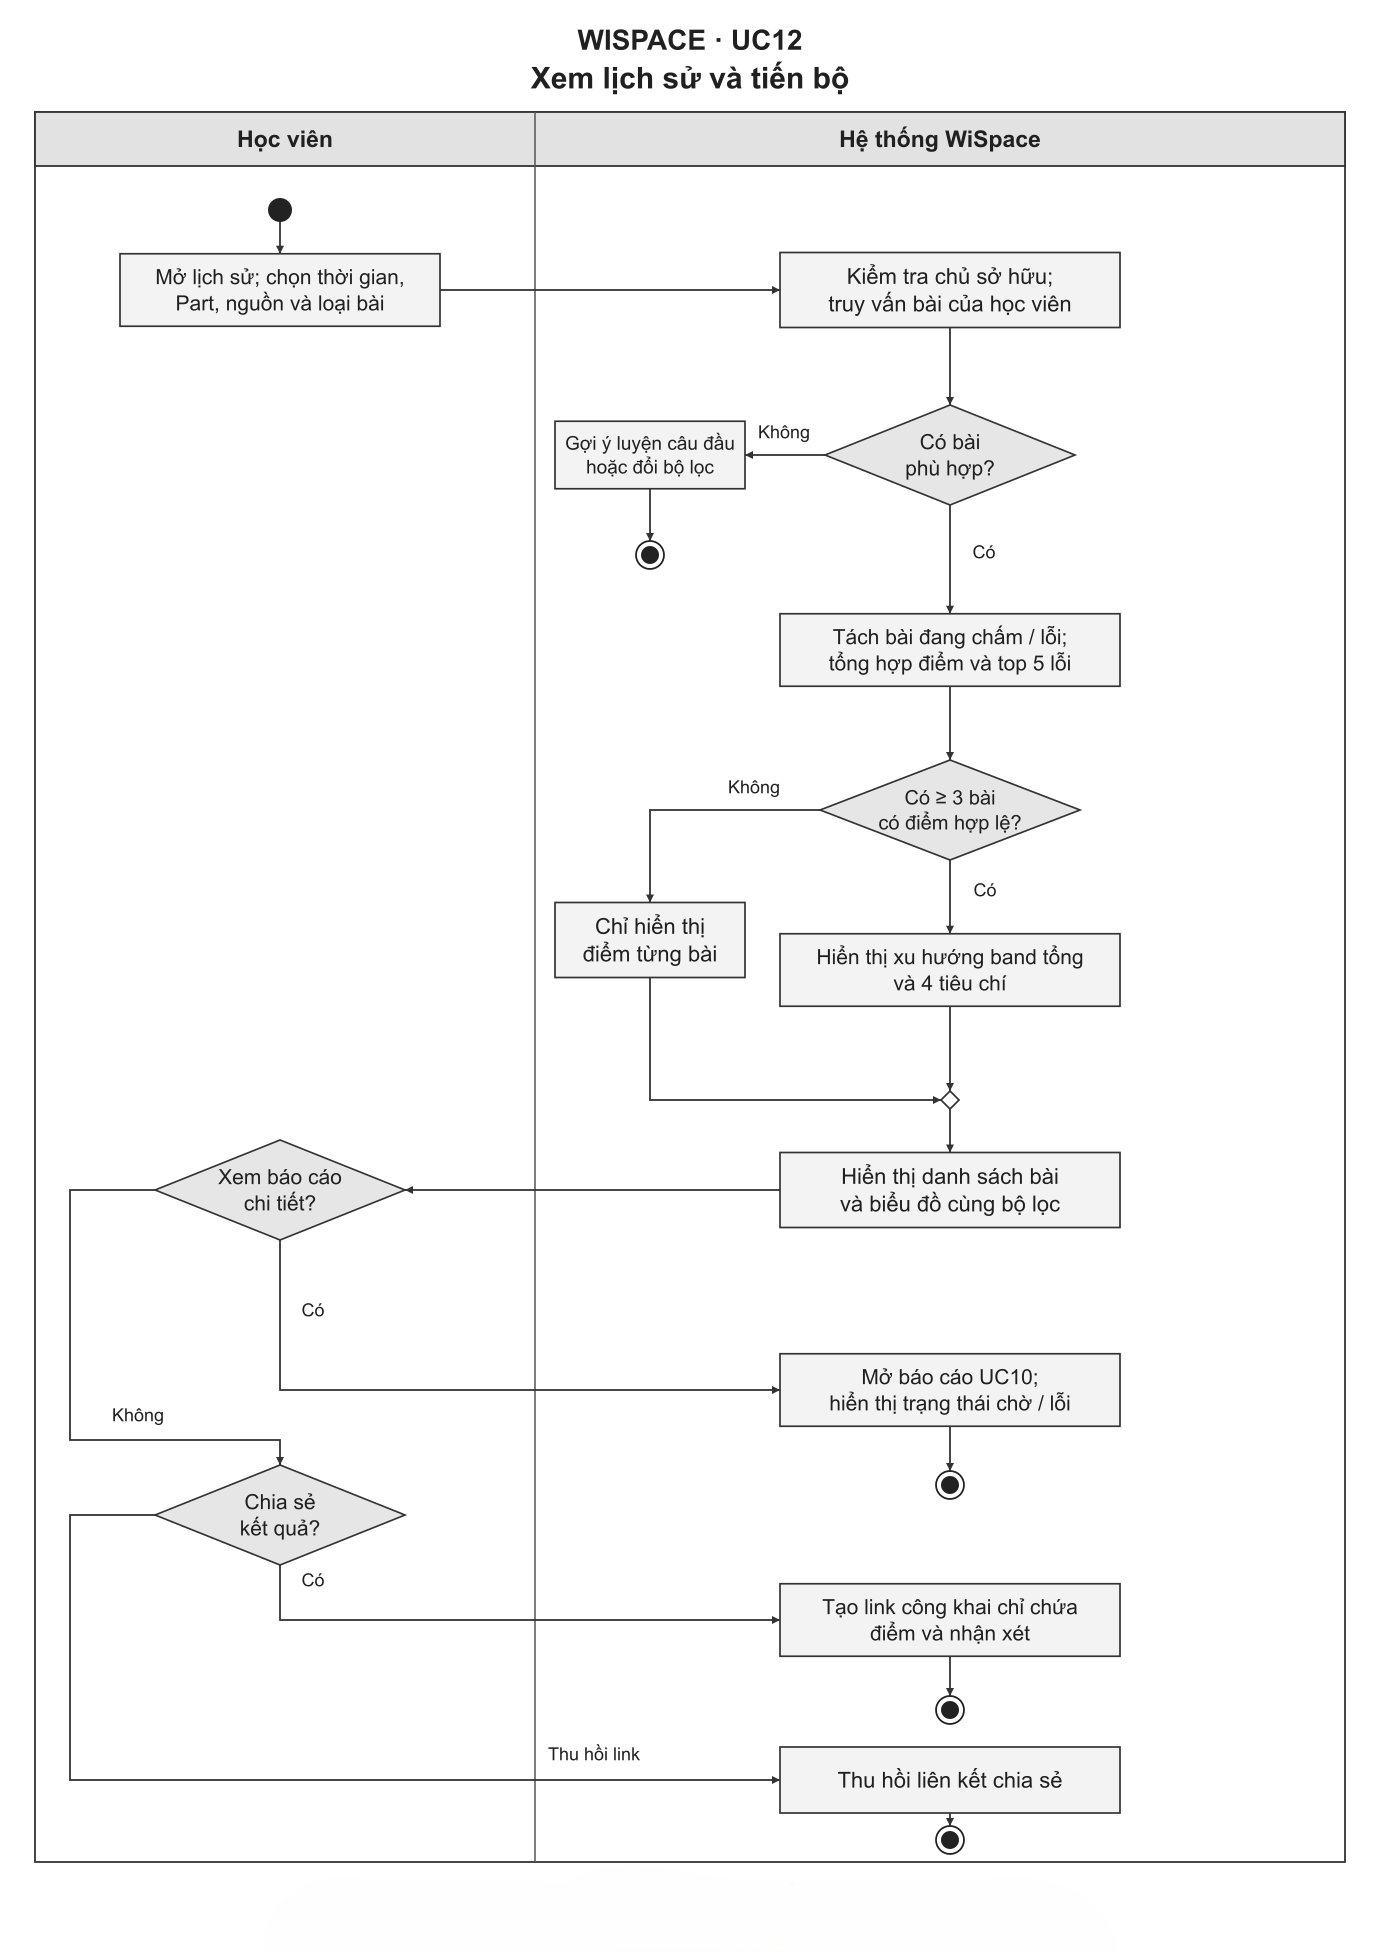
\includegraphics[width=\linewidth,height=0.72\textheight,keepaspectratio]{Images/Activity/Wispace/activity_uc12_progress_history.png}
    \caption{Sơ đồ hoạt động Wispace -- Use-case 12: Xem lịch sử và tiến bộ}
    \label{wispace:fig:activity_uc12}
\end{figure}

Học viên mở lịch sử và chọn bộ lọc. Hệ thống mở báo cáo, tạo hoặc thu hồi liên kết theo lựa chọn.
% activity-generated:end


\clearpage
\subsubsection{Sơ đồ luồng dữ liệu DFD}
\label{wispace:sec:dfd}

Phần này trình bày sơ đồ ngữ cảnh và DFD mức 1 của Wispace Speaking, tập trung vào dữ liệu tài khoản, kho đề, bài làm, kết quả và gói dịch vụ. Frontend, backend, hàng đợi và kho dữ liệu thuộc phạm vi hệ thống; các dịch vụ xác thực, TTS, chấm Speaking và thanh toán được xem là tác nhân ngoài.

Luồng dữ liệu được tổ chức quanh các nhóm nghiệp vụ dưới đây. Mã E, P và D chỉ có ý nghĩa trong phạm vi từng hệ thống.

\begin{longtable}{|>{\raggedright\arraybackslash}p{0.07\linewidth}|>{\raggedright\arraybackslash}p{0.25\linewidth}|p{0.58\linewidth}|}
\caption{Tác nhân ngoài của Wispace Speaking}\label{wispace:tab:dfd-entities}\\
\hline
\textbf{Mã} & \textbf{Tác nhân} & \textbf{Dữ liệu trao đổi} \\
\hline
\endfirsthead
\hline
\textbf{Mã} & \textbf{Tác nhân} & \textbf{Dữ liệu trao đổi} \\
\hline
\endhead
E1 & Khách / Học viên & Cung cấp thông tin tài khoản, bộ lọc đề, audio, yêu cầu xem kết quả và thanh toán; nhận nội dung luyện tập, báo cáo và quyền lợi sử dụng. \\
\hline
E2 & Moderator / Admin & Cung cấp dữ liệu đề, quyết định kiểm duyệt, thay đổi người dùng và cấu hình gói; nhận danh sách, trạng thái xử lý và nhật ký. \\
\hline
E3 & Email / Google OAuth & Tiếp nhận nội dung gửi OTP hoặc yêu cầu xác minh Google; trả trạng thái gửi hoặc thông tin danh tính. OTP do người dùng nhập thuộc luồng E1. \\
\hline
E4 & Dịch vụ TTS & Nhận văn bản câu hỏi và lựa chọn giọng; trả audio câu hỏi hoặc thông tin lỗi. \\
\hline
E5 & Scoring Model & Nhận audio và ngữ cảnh câu hỏi; trả transcript, điểm theo tiêu chí, lỗi và nhận xét. \\
\hline
E6 & PayOS & Nhận dữ liệu đơn thanh toán; trả liên kết thanh toán và trạng thái giao dịch đã xác minh. \\
\hline
\end{longtable}


\begin{longtable}{|>{\raggedright\arraybackslash}p{0.07\linewidth}|p{0.48\linewidth}|p{0.35\linewidth}|}
\caption{Tiến trình mức 1 của Wispace Speaking}\label{wispace:tab:dfd-processes}\\
\hline
\textbf{Mã} & \textbf{Tiến trình} & \textbf{Phạm vi} \\
\hline
\endfirsthead
\hline
\textbf{Mã} & \textbf{Tiến trình} & \textbf{Phạm vi} \\
\hline
\endhead
P1 & Xác thực và quản lý hồ sơ & UC01--UC04 \\
\hline
P2 & Tra cứu và quản lý kho đề & UC06--UC08 \\
\hline
P3 & Tiếp nhận bài và chấm Speaking & UC09, UC11 \\
\hline
P4 & Tổng hợp kết quả và tiến bộ & UC10, UC12 \\
\hline
P5 & Quản trị người dùng và gói dịch vụ & UC05; gói dịch vụ ở Chương 5 \\
\hline
\end{longtable}


\begin{longtable}{|>{\raggedright\arraybackslash}p{0.07\linewidth}|p{0.25\linewidth}|p{0.58\linewidth}|}
\caption{Kho dữ liệu của Wispace Speaking}\label{wispace:tab:dfd-stores}\\
\hline
\textbf{Mã} & \textbf{Kho dữ liệu} & \textbf{Nội dung} \\
\hline
\endfirsthead
\hline
\textbf{Mã} & \textbf{Kho dữ liệu} & \textbf{Nội dung} \\
\hline
\endhead
D1 & Tài khoản và phiên & Thông tin tài khoản, hồ sơ, vai trò, trạng thái, OTP và dữ liệu phiên xác thực. \\
\hline
D2 & Kho đề Speaking & Câu hỏi, chủ đề, nguồn đề, trạng thái kiểm duyệt, báo cáo đề và audio câu hỏi. \\
\hline
D3 & Bài làm và kết quả & Phiên luyện tập/thi thử, audio câu trả lời, trạng thái chấm, điểm, transcript, lỗi, tiến bộ và liên kết chia sẻ. \\
\hline
D4 & Gói, quota, thanh toán & Gói dịch vụ, quyền lợi, định mức, bút toán sử dụng/hoàn quota và giao dịch thanh toán. \\
\hline
D5 & Nhật ký quản trị & Người thực hiện, lý do, thời điểm và nội dung thay đổi người dùng hoặc cấu hình gói. \\
\hline
\end{longtable}


\clearpage

\paragraph{Sơ đồ ngữ cảnh.}

Sơ đồ thể hiện toàn bộ Wispace Speaking như một tiến trình duy nhất; các mũi tên ghi rõ dữ liệu gửi đến và dữ liệu trả về cho từng tác nhân ngoài.

\begin{figure}[H]
\centering
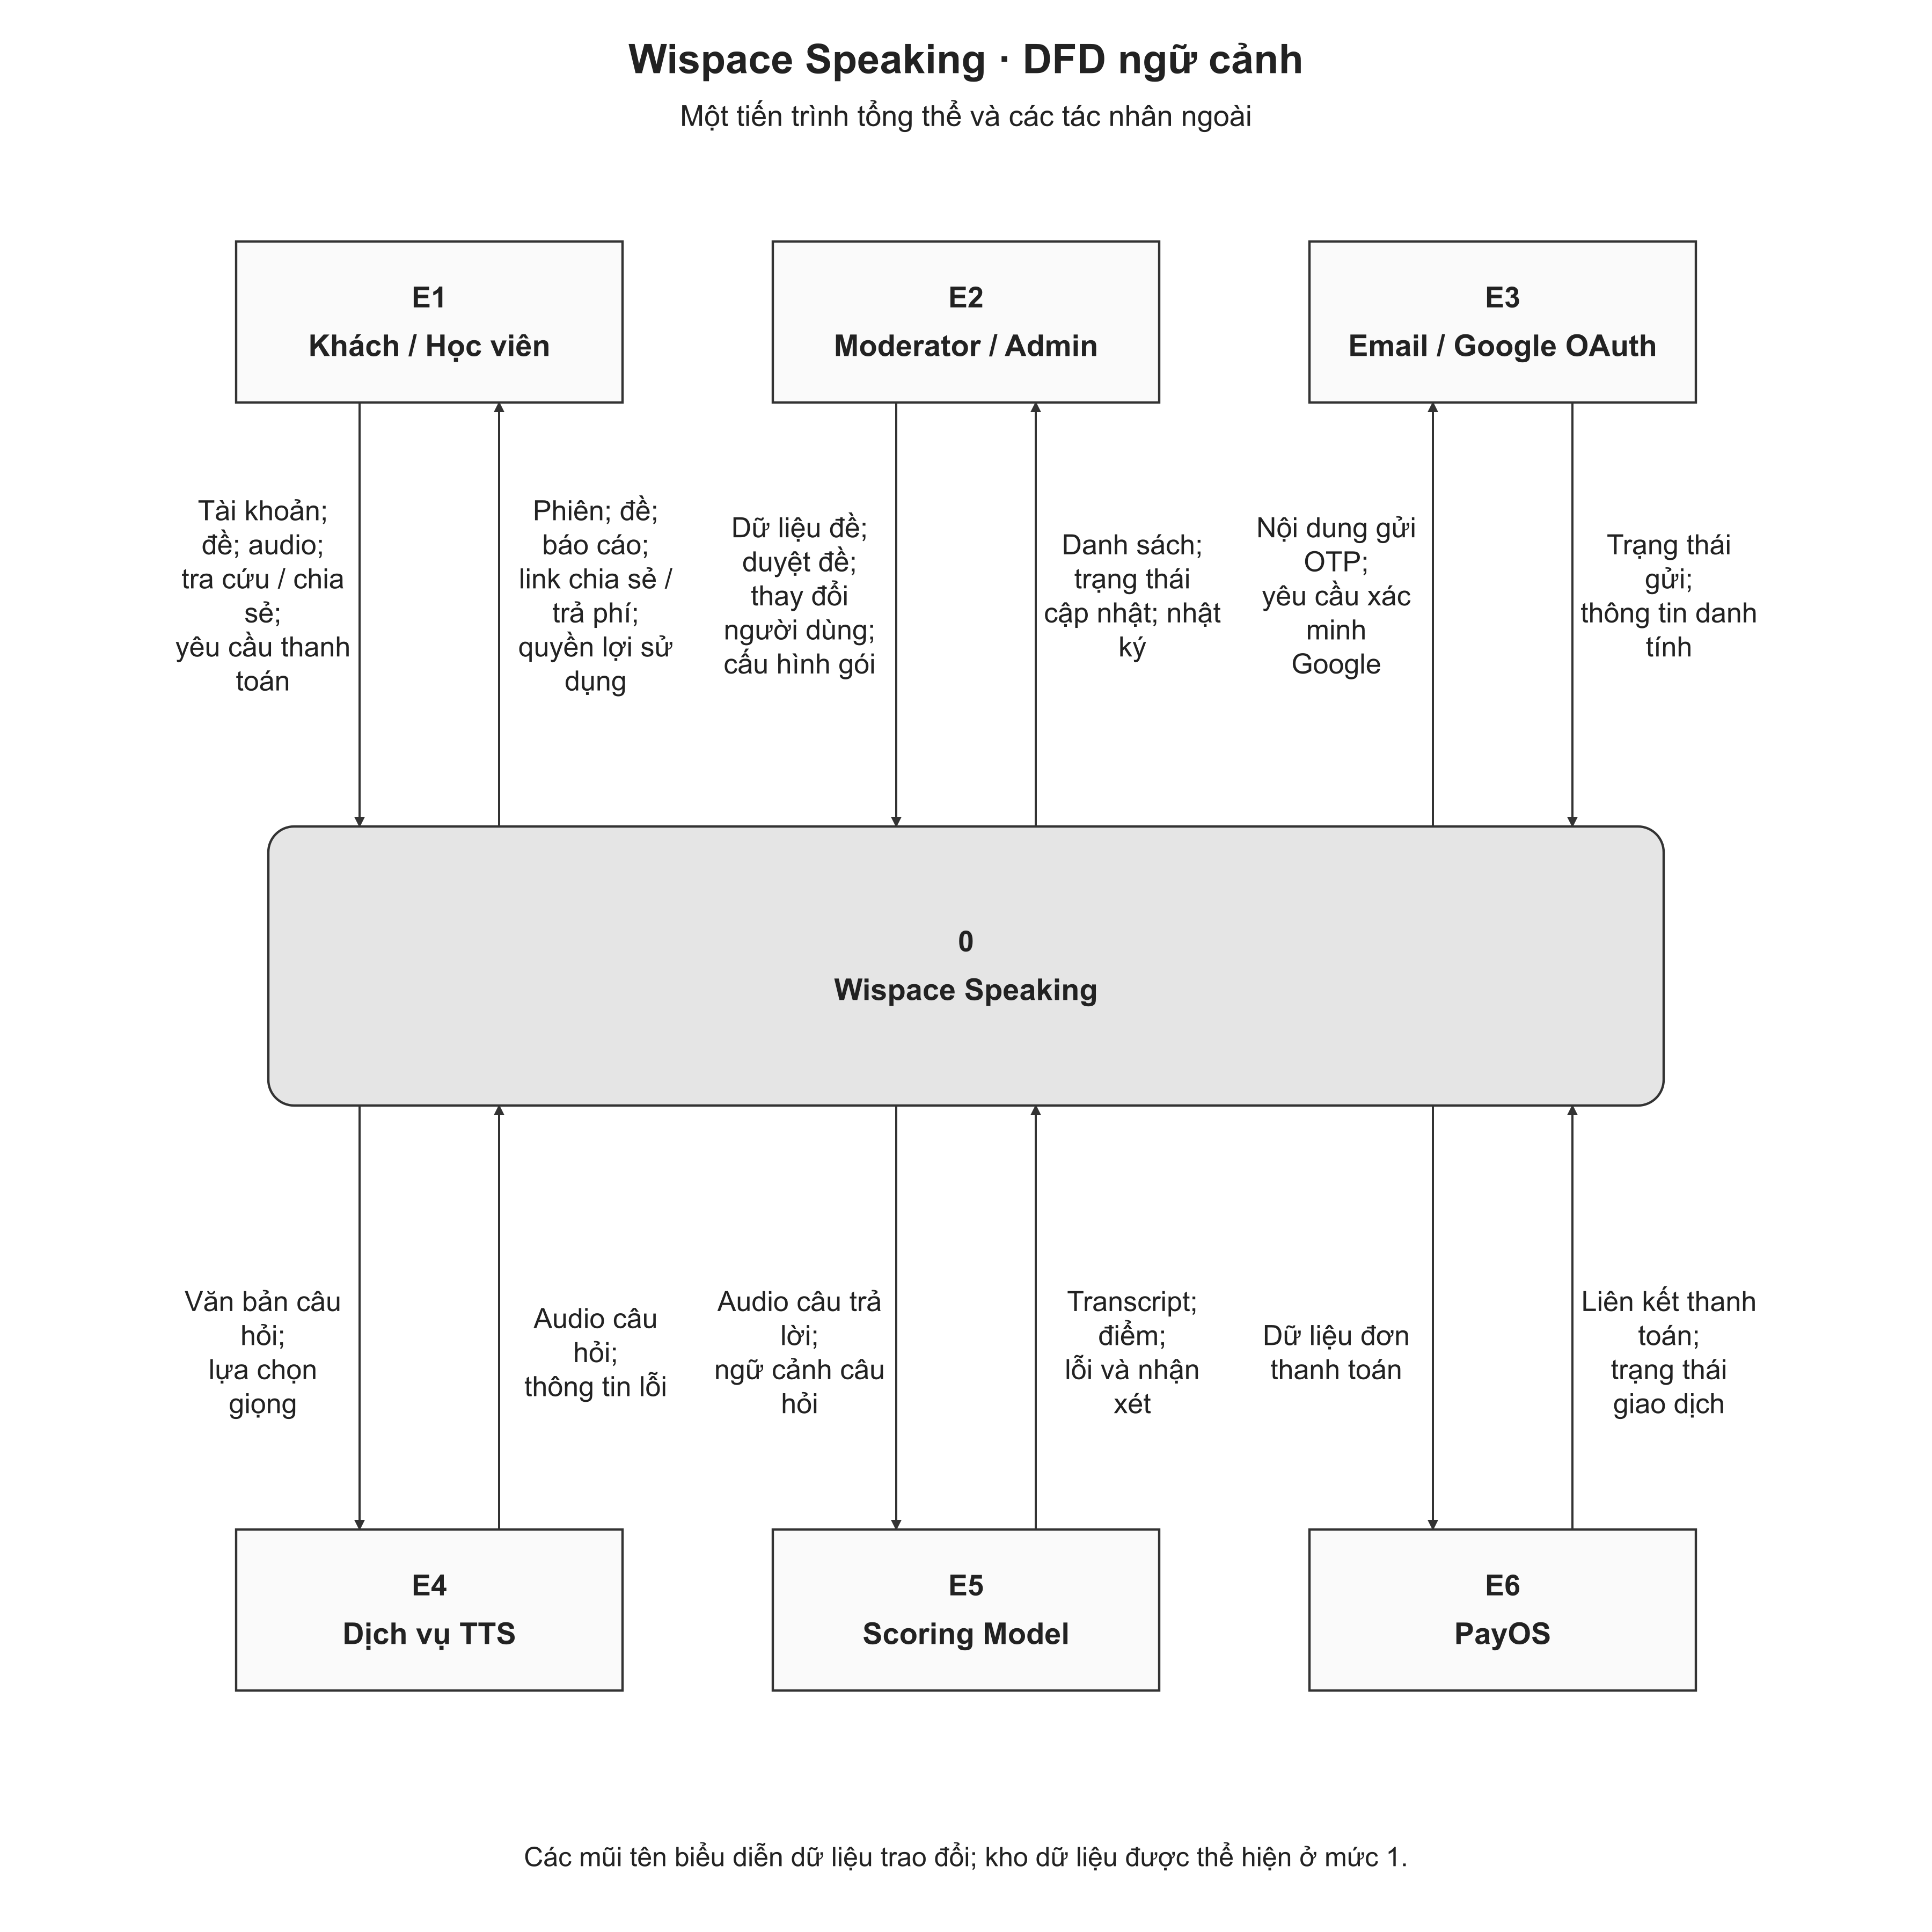
\includegraphics[width=\linewidth,height=0.78\textheight,keepaspectratio]{Images/DFD/Wispace/wispace_dfd_context.png}
\caption{DFD ngữ cảnh của Wispace Speaking}
\label{wispace:fig:dfd-context}
\end{figure}

\clearpage


\paragraph{Sơ đồ mức 1.}

Để giữ nhãn và đường nối dễ đọc, cùng một sơ đồ mức 1 được trình bày thành hai phần. Các tác nhân và kho dữ liệu có cùng mã ở hai phần là cùng một đối tượng logic. Dữ liệu giữa các nhóm xử lý được trao đổi qua kho dùng chung, không phải các bản sao tách biệt.

\clearpage

\begin{figure}[H]
\centering
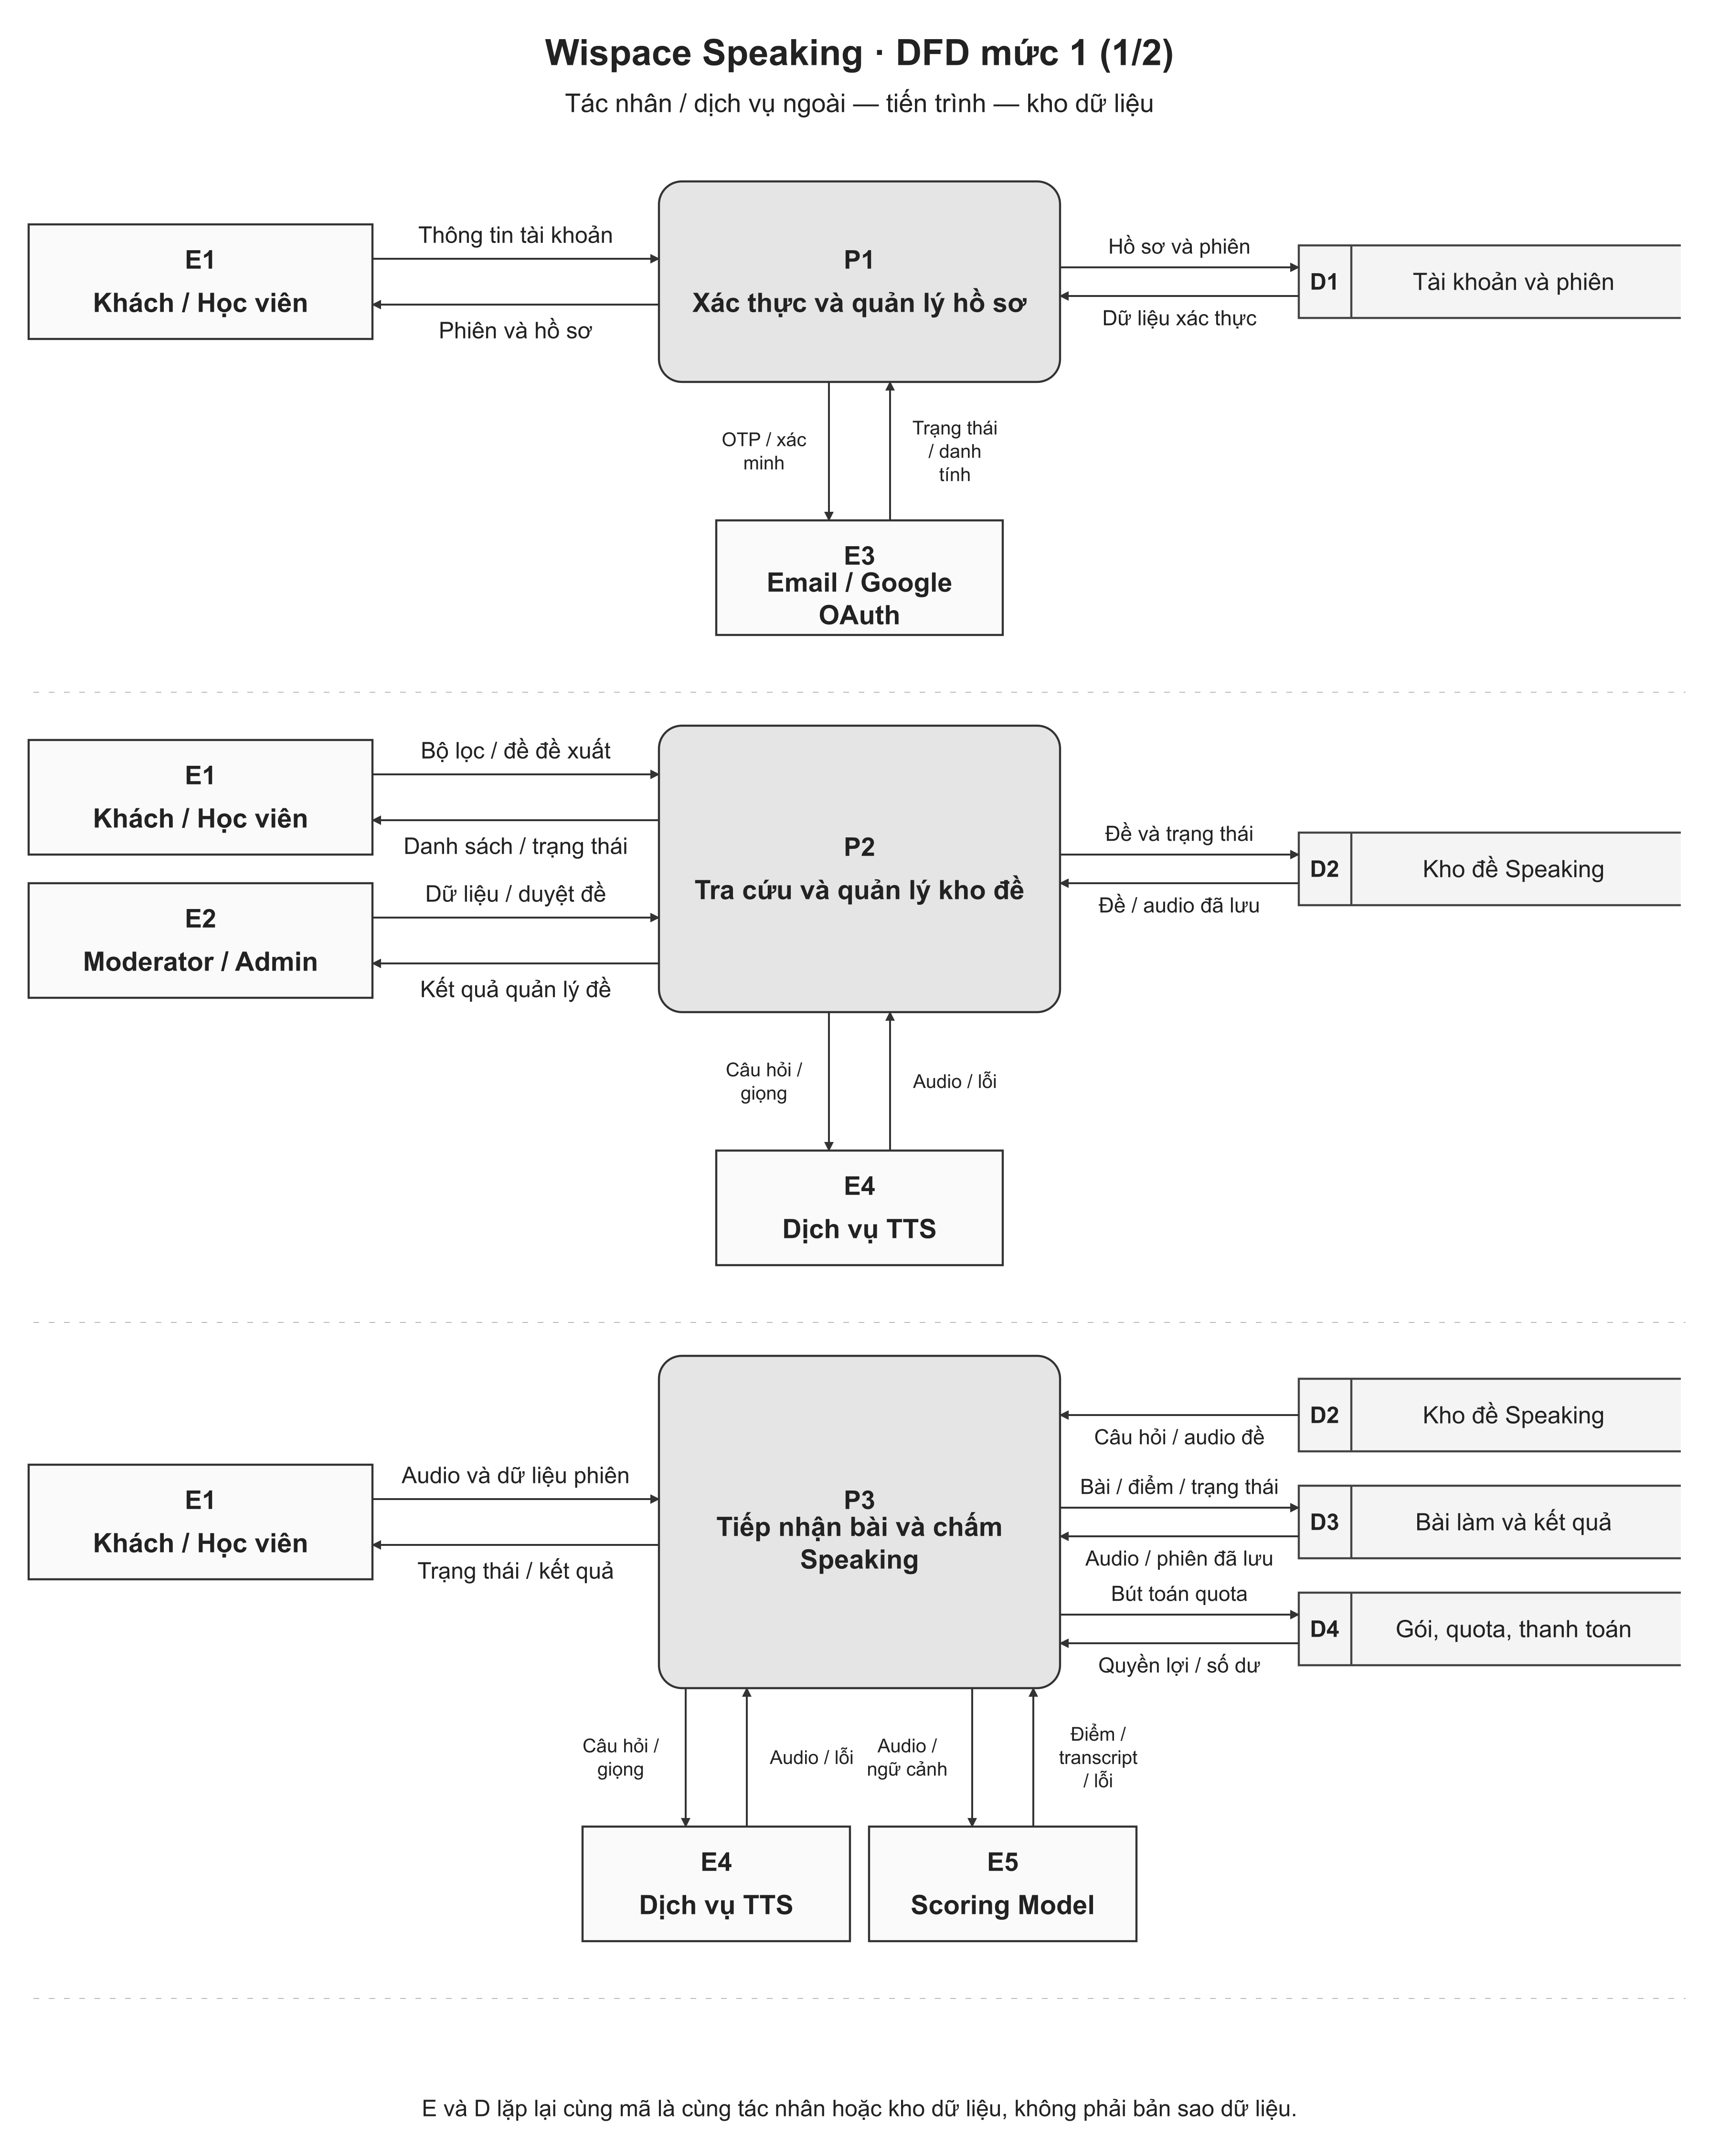
\includegraphics[width=\linewidth,height=0.78\textheight,keepaspectratio]{Images/DFD/Wispace/wispace_dfd_level1_1.png}
\caption{DFD mức 1 của Wispace Speaking: P1, P2, P3}
\label{wispace:fig:dfd-level1-1}
\end{figure}

\clearpage

\begin{figure}[H]
\centering
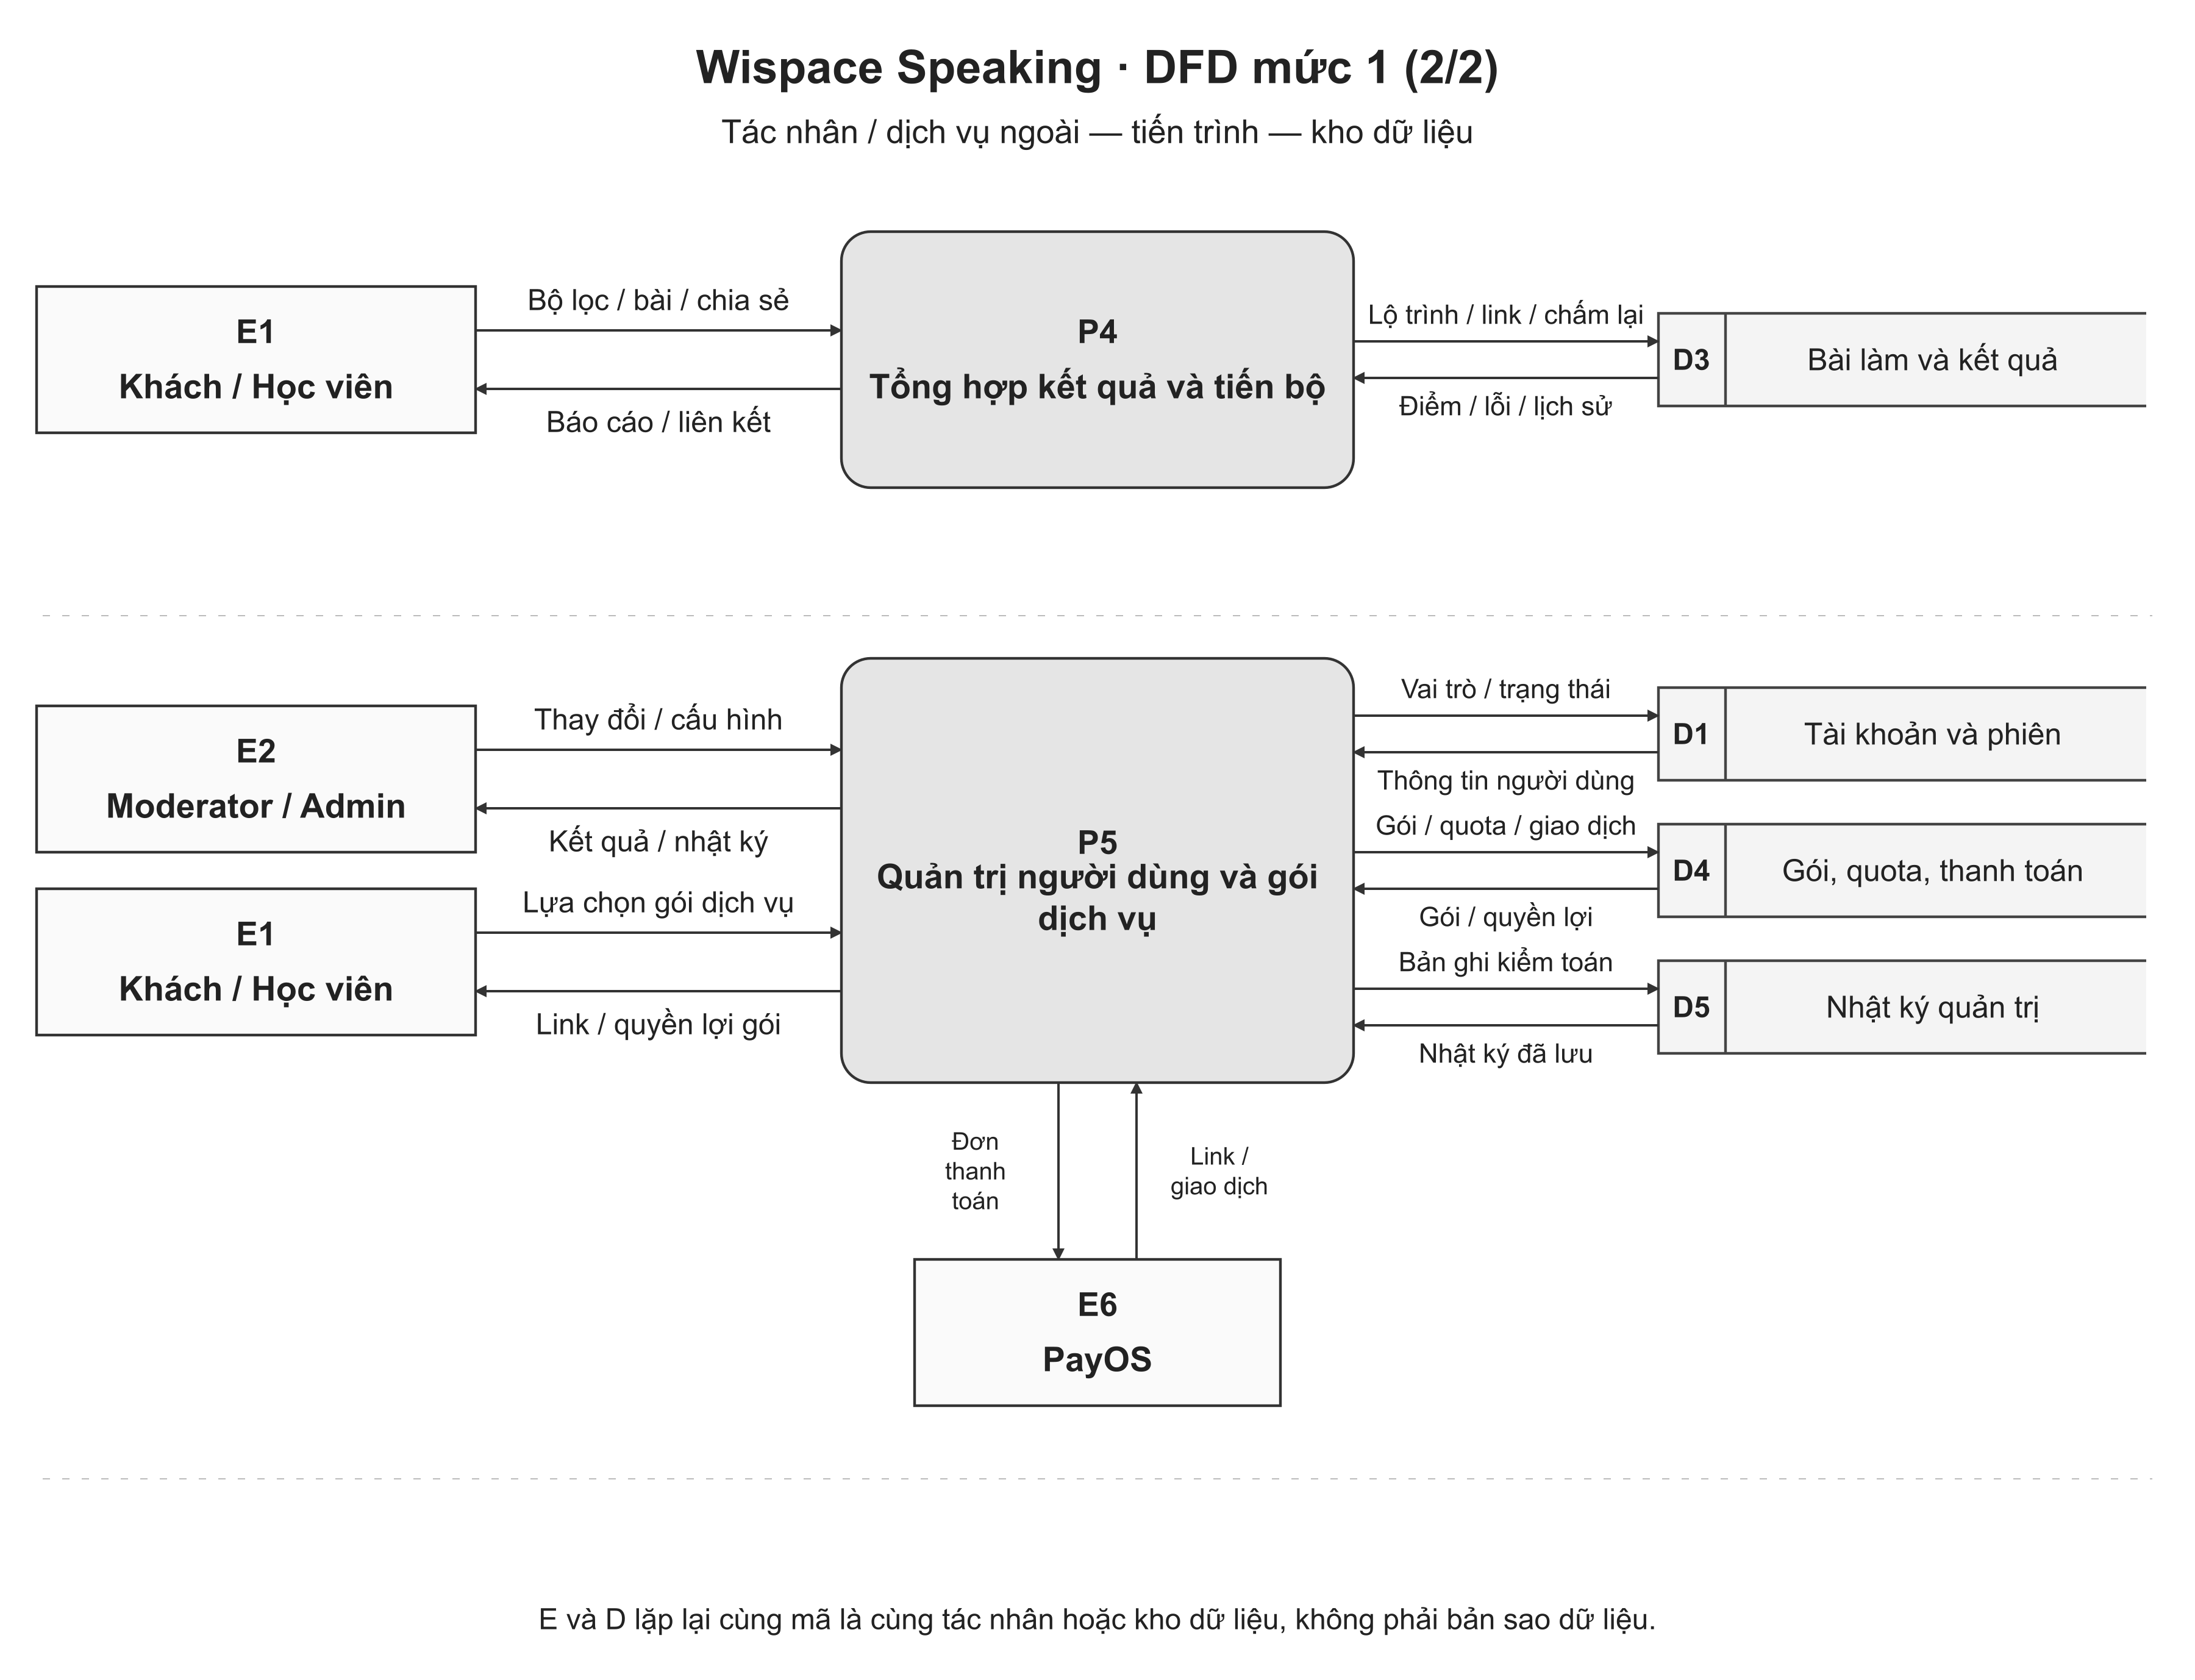
\includegraphics[width=\linewidth,height=0.78\textheight,keepaspectratio]{Images/DFD/Wispace/wispace_dfd_level1_2.png}
\caption{DFD mức 1 của Wispace Speaking: P4, P5}
\label{wispace:fig:dfd-level1-2}
\end{figure}




P3 đọc câu hỏi từ D2, ghi audio và kết quả vào D3, đồng thời cập nhật bút toán quota ở D4. P4 dùng dữ liệu D3 để lập báo cáo, thống kê tiến bộ và quản lý liên kết chia sẻ; yêu cầu chấm lại được ghi vào trạng thái bài làm ở D3 để P3 xử lý. P5 bao gồm yêu cầu mua gói đã nêu ở Chương 5, ngoài phạm vi 12 use-case chi tiết.


\clearpage
\subsection{Hệ thống AIHub}

\subsubsection{Lược đồ Use-case tổng quan}
Toàn bộ hệ thống AIHub bao gồm 20 use-case chính, được phân chia thành 3 phân vùng chức năng cốt lõi như minh họa tại Hình~\ref{aihub:fig:aihub_usecase_overview}:
\textbf{Phân hệ Cổng API Gateway \& Developer Portal:} Bao gồm các chức năng Đăng nhập/Xác thực, Quản lý khóa API, Tra cứu hạn mức và sử dụng cURL Sandbox. \textbf{Phân hệ Quản trị \& Điều hành:} Bao gồm Quản lý thành viên tổ chức, Cấu hình gói và hạn mức, Quản lý danh mục đặc tả Universal Specs, Kiểm tra trạng thái hệ thống và Xem nhật ký kiểm toán.
\begin{figure}[H]
    \centering
    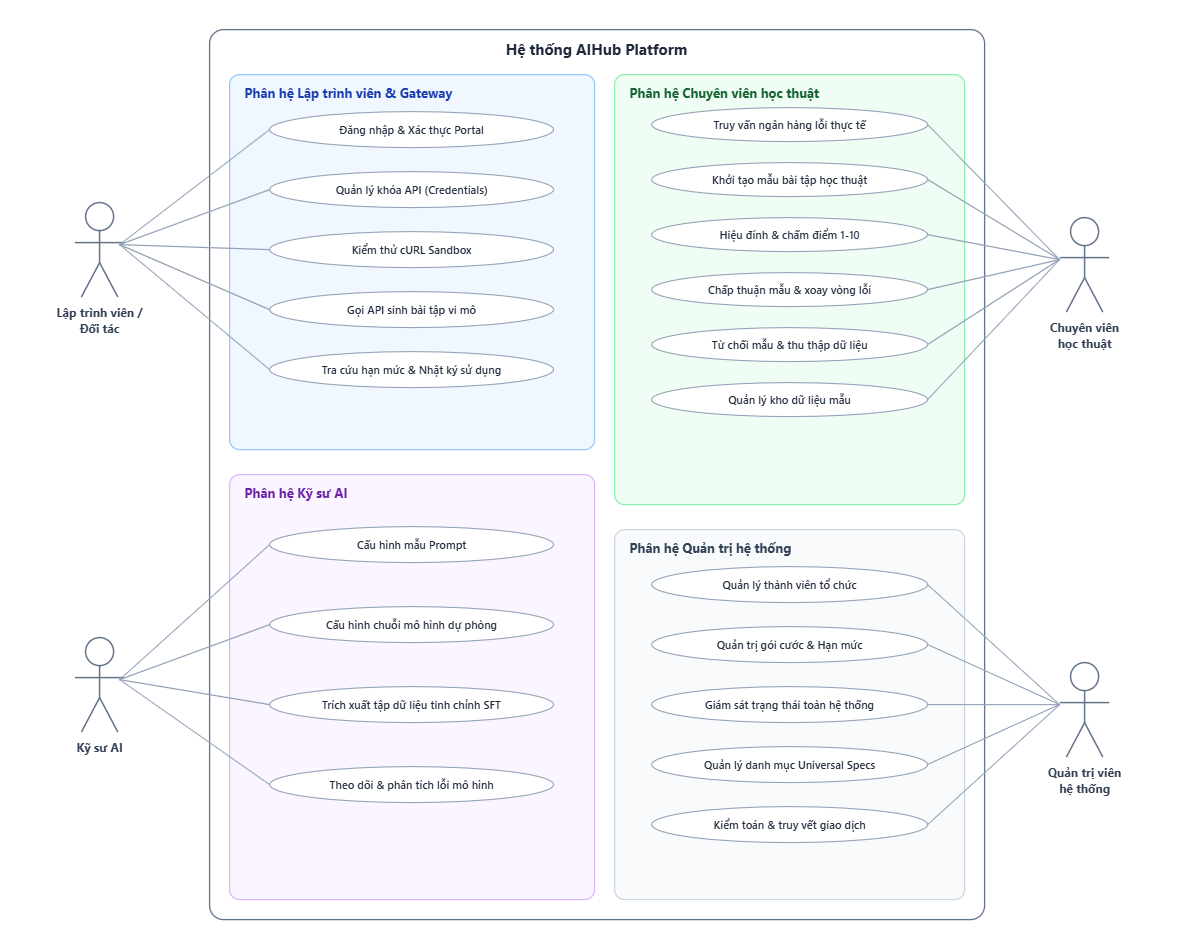
\includegraphics[width=1\textwidth]{Images/Usecase/AIHub/aihub_usecase.png}
    \caption{Sơ đồ Use-case tổng quan hệ thống AIHub Platform}
    \label{aihub:fig:aihub_usecase_overview}
\end{figure}
\newpage

\subsubsection{Đặc tả các Use-case chi tiết}
\setcounter{paragraph}{0}                      % Đặt lại bộ đếm về 0
\renewcommand{\theparagraph}{\alph{paragraph}}  % Chuyển số thành chữ cái thường a, b, c...

Các bảng dưới đây đặc tả 20 use-case của AIHub. Mỗi bảng mô tả tác nhân, điều kiện trước và sau, luồng chính, luồng thay thế và các trường hợp ngoại lệ.

% =========================================================================
% NHÓM 1: LẬP TRÌNH VIÊN / ĐỐI TÁC TÍCH HỢP
% =========================================================================

\paragraph{Use-case 1: Đăng nhập và Xác thực Portal}

\begingroup
\small
\begin{longtable}{|p{3.2cm}|p{\dimexpr\linewidth-3.2cm-4\tabcolsep-3\arrayrulewidth\relax}|}
\caption{Đặc tả use-case Đăng nhập và Xác thực Portal}
\label{aihub:tab:uc_dev_auth}\\
\hline
\textbf{Tác nhân} & Lập trình viên / Đối tác tích hợp, Máy chủ xác thực (Session Service) \\ \hline
\textbf{Điều kiện trước} & Hệ thống hoạt động bình thường; lập trình viên đã có tài khoản được kích hoạt trong bảng \texttt{users}. \\ \hline
\textbf{Điều kiện sau} & Phiên làm việc được thiết lập qua Session Cookie an toàn; lập trình viên được chuyển tới Bảng điều khiển nhà phát triển. \\ \hline
\textbf{Luồng chính} & 1. Người dùng mở Portal, nhập email và mật khẩu.\newline 2. Hệ thống kiểm tra đầu vào, mật khẩu băm, trạng thái tài khoản, vai trò và tổ chức.\newline 3. Hệ thống tạo phiên bằng cookie bảo mật và mở Dashboard. \\ \hline
\textbf{Luồng thay thế} &
\textbf{Nhánh 1: Đăng xuất khỏi hệ thống (Logout)}\newline 1.1. Lập trình viên chọn menu tài khoản và nhấn ``Đăng xuất''.\newline 1.2. Hệ thống thu hồi phiên làm việc, xóa cookie bảo mật trên trình duyệt và điều hướng về trang đăng nhập. \\ \hline
\textbf{Ngoại lệ} &
\textbf{Lỗi 1: Sai email hoặc mật khẩu}\newline Hệ thống hiển thị thông báo ``Thông tin đăng nhập không hợp lệ''. Nhập sai quá 5 lần liên tiếp sẽ tạm khóa tài khoản 15 phút.\newline \textbf{Lỗi 2: Tài khoản bị khóa}\newline Trả về thông báo tài khoản đang bị vô hiệu hóa kèm chỉ dẫn liên hệ Quản trị viên. \\ \hline
\end{longtable}
\endgroup
\paragraph{Use-case 2: Quản lý khóa API}

\begingroup
\small
\begin{longtable}{|p{3.2cm}|p{\dimexpr\linewidth-3.2cm-4\tabcolsep-3\arrayrulewidth\relax}|}
\caption{Đặc tả use-case Quản lý khóa API}
\label{aihub:tab:uc_manage_credentials}\\
\hline
\textbf{Tác nhân} & Lập trình viên, Quản trị viên tổ chức \\ \hline
\textbf{Điều kiện trước} & Người dùng đã đăng nhập với vai trò hợp lệ trong tổ chức. \\ \hline
\textbf{Điều kiện sau} & Cặp mã chứng thực được cập nhật trong bảng \texttt{credentials}; khóa bí mật mới chỉ được hiển thị duy nhất 1 lần. \\ \hline
\textbf{Luồng chính} & 1. Người dùng chọn tạo hoặc xoay vòng khóa.\newline 2. Hệ thống kiểm tra quyền và giới hạn gói, sinh clientId có tiền tố môi trường và secretKey ngẫu nhiên.\newline 3. Bí mật được băm bằng Bcrypt; credentials được lưu theo tổ chức.\newline 4. Hệ thống hiển thị bí mật một lần để người dùng sao chép và xác nhận. \\ \hline
\textbf{Luồng thay thế} &
\textbf{Nhánh 1: Thu hồi hoặc vô hiệu hóa khóa (Revoke Key)}\newline Lập trình viên chọn một khóa đang hoạt động và nhấn ``Xóa khóa''. Hệ thống đánh dấu vô hiệu hóa; mọi yêu cầu sử dụng khóa này sẽ bị Gateway từ chối ngay lập tức. \\ \hline
\textbf{Ngoại lệ} &
\textbf{Lỗi 1: Vượt quá số lượng khóa cho phép của gói cước}\newline Nếu tổ chức thuộc gói Free Sandbox và đã đạt giới hạn 2 khóa, hệ thống từ chối tạo mới và yêu cầu nâng cấp gói cước. \\ \hline
\end{longtable}
\endgroup

\paragraph{Use-case 3: Kiểm thử cURL Sandbox}

\begingroup
\small
\begin{longtable}{|p{3.2cm}|p{\dimexpr\linewidth-3.2cm-4\tabcolsep-3\arrayrulewidth\relax}|}
\caption{Đặc tả use-case Kiểm thử cURL Sandbox}
\label{aihub:tab:uc_run_spec_curl}\\
\hline
\textbf{Tác nhân} & Lập trình viên / Đối tác tích hợp \\ \hline
\textbf{Điều kiện trước} & Lập trình viên đã mở trang Universal AI Spec Catalog; đặc tả dịch vụ đã được tải. \\ \hline
\textbf{Điều kiện sau} & Nhận kết quả phản hồi JSON, thời gian xử lý (latency), số token tiêu thụ và trạng thái kiểm định tính hợp lệ của lược đồ. \\ \hline
\textbf{Luồng chính} & 1. Lập trình viên chọn dịch vụ, xem đặc tả và nhập JSON yêu cầu.\newline 2. Hệ thống thực thi dịch vụ nội bộ; dịch vụ đối tác chưa tích hợp dùng mô phỏng có kiểm định schema với độ trễ 300--800 ms.\newline 3. Hệ thống hiển thị mã HTTP, JSON, thời gian xử lý, token và kết quả kiểm định schema. \\ \hline
\textbf{Luồng thay thế} & Không có. \\ \hline
\textbf{Ngoại lệ} &
\textbf{Lỗi 1: Dữ liệu JSON gửi đi sai cú pháp}\newline Giao diện cảnh báo lỗi cú pháp JSON và khóa nút gửi yêu cầu.\newline \textbf{Lỗi 2: Cấu trúc phản hồi không khớp lược đồ chuẩn}\newline Hệ thống hiển thị cờ cảnh báo \texttt{validation.valid = false} kèm danh sách chi tiết các trường bị thiếu hoặc sai kiểu dữ liệu. \\ \hline
\end{longtable}
\endgroup

\paragraph{Use-case 4: Gọi API sinh bài tập vi mô}

\begingroup
\small
\begin{longtable}{|p{3.2cm}|p{\dimexpr\linewidth-3.2cm-4\tabcolsep-3\arrayrulewidth\relax}|}
\caption{Đặc tả use-case Gọi API sinh bài tập vi mô}
\label{aihub:tab:uc_create_exercise}\\
\hline
\textbf{Tác nhân} & Ứng dụng WISPACE / Lập trình viên, Composite LLM Adapter \\ \hline
\textbf{Điều kiện trước} & Header yêu cầu chứa mã \textit{x-client-id} và \textit{x-secret-key} hợp lệ; tổ chức còn hạn ngạch gọi API trong tháng. \\ \hline
\textbf{Điều kiện sau} & Bài tập được khởi tạo hoàn chỉnh với câu hỏi, đáp án, giải thích chi tiết và rubric chấm điểm; số liệu được ghi vào \texttt{usage\_logs}. \\ \hline
\textbf{Luồng chính} & 1. Gateway xác thực credentials, quyền dịch vụ, RPM và hạn mức.\newline 2. Hệ thống kiểm tra dữ liệu và mã lỗi trong bộ 28 lỗi IELTS.\newline 3. Hệ thống lấy dẫn chứng theo chủ đề, gọi mô hình sinh bài tập và chuẩn hóa kết quả.\newline 4. Phản hồi gồm câu hỏi, đáp án, giải thích, rubric và metadata mô hình/thời gian/token; usage được ghi nhận. \\ \hline
\textbf{Luồng thay thế} &
\textbf{Nhánh 1: Sinh dạng bài tự luận ngắn (Short Writing)}\newline Hệ thống tự động đính kèm tiêu chí chấm điểm chi tiết \textit{ai\_grading\_rubric} trên thang điểm 1--10 và câu trả lời mẫu chuẩn Band 8.0+. \\ \hline
\textbf{Ngoại lệ} &
\textbf{Lỗi 1: Mã lỗi không thuộc bộ phân loại 28 lỗi IELTS}\newline Ném lỗi miền \texttt{InvalidErrorCodeError}, trả về mã HTTP 400 Bad Request.\newline \textbf{Lỗi 2: Dịch vụ AI chính gặp sự cố kết nối hoặc quá thời gian chờ}\newline Kích hoạt chuỗi dự phòng (Fallback Chain): tự động chuyển sang Google Gemini $\rightarrow$ OpenAI GPT-4o $\rightarrow$ Động cơ Ngoại tuyến (Deterministic Engine). \\ \hline
\end{longtable}
\endgroup

\paragraph{Use-case 5: Tra cứu hạn mức và Nhật ký sử dụng}

\begingroup
\small
\begin{longtable}{|p{3.2cm}|p{\dimexpr\linewidth-3.2cm-4\tabcolsep-3\arrayrulewidth\relax}|}
\caption{Đặc tả use-case Tra cứu hạn mức và Nhật ký sử dụng}
\label{aihub:tab:uc_view_usage_logs}\\
\hline
\textbf{Tác nhân} & Lập trình viên, Quản trị viên tổ chức \\ \hline
\textbf{Điều kiện trước} & Người dùng đã đăng nhập và thuộc một tổ chức có mã khóa truy cập. \\ \hline
\textbf{Điều kiện sau} & Bảng chỉ số tiêu thụ, biểu đồ trực quan và nhật ký giao dịch được hiển thị đầy đủ. \\ \hline
\textbf{Luồng chính} & 1. Người dùng mở mục sử dụng dịch vụ.\newline 2. Hệ thống hiển thị hạn mức tháng đã dùng/còn lại và trần RPM.\newline 3. Hệ thống tổng hợp lưu lượng, mã HTTP, độ trễ và token theo ngày.\newline 4. Người dùng xem nhật ký gồm thời điểm, endpoint, phương thức, thời lượng, token, IP và trạng thái. \\ \hline
\textbf{Luồng thay thế} &
\textbf{Nhánh 1: Lọc nhật ký theo tiêu chí nâng cao}\newline Người dùng lọc danh sách giao dịch theo khoảng ngày, theo mã khóa \textit{clientId} cụ thể, hoặc chỉ hiển thị các yêu cầu gặp lỗi (mã $4xx$, $5xx$). \\ \hline
\textbf{Ngoại lệ} &
\textbf{Lỗi 1: Định ngạch chạm ngưỡng cảnh báo ($\ge 80\%$ hoặc $100\%$)}\newline Hệ thống hiển thị thanh thông báo màu đỏ cảnh báo tổ chức sắp hoặc đã dùng hết định ngạch gọi API trong tháng, đề xuất nâng cấp gói cước. \\ \hline
\end{longtable}
\endgroup

% =========================================================================
% NHÓM 2: CHUYÊN VIÊN HỌC THUẬT (ACADEMIC LAB)
% =========================================================================

\paragraph{Use-case 6: Truy vấn ngân hàng lỗi thực tế}

\begingroup
\small
\begin{longtable}{|p{3.2cm}|p{\dimexpr\linewidth-3.2cm-4\tabcolsep-3\arrayrulewidth\relax}|}
\caption{Đặc tả use-case Truy vấn ngân hàng lỗi thực tế}
\label{aihub:tab:uc_query_references}\\
\hline
\textbf{Tác nhân} & Chuyên viên học thuật, WISPACE Reference API / DB Adapter \\ \hline
\textbf{Điều kiện trước} & Chuyên viên đã đăng nhập vào Academic Lab Workbench; kho dẫn chứng khả dụng. \\ \hline
\textbf{Điều kiện sau} & Danh sách các trích dẫn lỗi bài thi kèm đề bài và nhận xét chuyên môn được trả về. \\ \hline
\textbf{Luồng chính} & 1. Chuyên viên chọn Task 1/2, tiêu chí TR/CC/LR/GRA, mã lỗi, chủ đề và số dẫn chứng.\newline 2. Hệ thống kiểm tra tham số và truy vấn API dẫn chứng Wispace.\newline 3. Kết quả gồm đề bài, loại câu hỏi, trích dẫn, ảnh biểu đồ nếu có và nhận xét chuyên môn.\newline 4. Hệ thống chuẩn hóa và hiển thị dẫn chứng. \\ \hline
\textbf{Luồng thay thế} &
\textbf{Nhánh 1: Kết nối API ngoài gián đoạn, kích hoạt kho dẫn chứng nội bộ}\newline Nếu gọi API WISPACE thất bại hoặc quá thời gian chờ, hệ thống tự động chuyển sang \texttt{WispaceReferenceAdapter} để truy vấn trực tiếp từ bảng cơ sở dữ liệu cục bộ \texttt{wispace\_essay\_references} và tiếp tục bước 5. \\ \hline
\textbf{Ngoại lệ} &
\textbf{Lỗi 1: Không tìm thấy dẫn chứng phù hợp}\newline Trả về danh sách rỗng kèm thông báo đề xuất mở rộng phạm vi tìm kiếm hoặc chuyển sang chế độ sinh bài tập không dùng dẫn chứng thực tế. \\ \hline
\end{longtable}
\endgroup

\paragraph{Use-case 7: Khởi tạo mẫu bài tập học thuật}

\begingroup
\small
\begin{longtable}{|p{3.2cm}|p{\dimexpr\linewidth-3.2cm-4\tabcolsep-3\arrayrulewidth\relax}|}
\caption{Đặc tả use-case Khởi tạo mẫu bài tập học thuật}
\label{aihub:tab:uc_academic_generate}\\
\hline
\textbf{Tác nhân} & Chuyên viên học thuật, Composite LLM Adapter \\ \hline
\textbf{Điều kiện trước} & Chuyên viên đã đăng nhập hệ thống với quyền \textit{ACADEMIC\_SPECIALIST}. \\ \hline
\textbf{Điều kiện sau} & Bản ghi mẫu học thuật được tạo ở trạng thái DRAFT; dữ liệu AI thô được lưu trữ nguyên vẹn trong trường \textit{rawAiOutput}. \\ \hline
\textbf{Luồng chính} & 1. Chuyên viên chọn Task, tiêu chí, mã lỗi, dạng bài tập và nhập chỉ dẫn sư phạm.\newline 2. Hệ thống kiểm tra tham số, lấy dẫn chứng nếu được yêu cầu và dựng Prompt theo phiên bản.\newline 3. Mô hình sinh nội dung; hệ thống kiểm tra kết quả.\newline 4. Mẫu được lưu DRAFT với rawAiOutput nguyên vẹn và hiển thị để thẩm định. \\ \hline
\textbf{Luồng thay thế} &
\textbf{Nhánh 1: Sử dụng dẫn chứng tùy biến do chuyên viên nhập}\newline Chuyên viên tự nhập trực tiếp câu trích dẫn và phân tích lỗi của học sinh thay vì lấy tự động từ ngân hàng dữ liệu. \\ \hline
\textbf{Ngoại lệ} &
\textbf{Lỗi 1: Lỗi mô hình AI không tạo được nội dung hợp lệ}\newline Hệ thống hiển thị thông báo lỗi chi tiết, giữ nguyên các tham số cấu hình trên form và đề xuất chuyên viên thử lại. \\ \hline
\end{longtable}
\endgroup

\paragraph{Use-case 8: Kiểm định, hiệu đính và chấm điểm bài tập}

\begingroup
\small
\begin{longtable}{|p{3.2cm}|p{\dimexpr\linewidth-3.2cm-4\tabcolsep-3\arrayrulewidth\relax}|}
\caption{Đặc tả use-case Kiểm định, hiệu đính và chấm điểm bài tập}
\label{aihub:tab:uc_academic_review_score}\\
\hline
\textbf{Tác nhân} & Chuyên viên học thuật \\ \hline
\textbf{Điều kiện trước} & Mẫu bài tập đang mở ở trạng thái DRAFT; đã có dữ liệu \textit{rawAiOutput}. \\ \hline
\textbf{Điều kiện sau} & Bản hiệu đính hoàn chỉnh được lưu tạm trong trường \textit{finalOutput} kèm điểm số chất lượng (1--10). \\ \hline
\textbf{Luồng chính} & 1. Chuyên viên kiểm tra câu hỏi, đáp án và giải thích trong rawAiOutput.\newline 2. Chuyên viên hiệu đính finalOutput, nhập điểm chất lượng bản gốc 1--10 và reviewedBy.\newline 3. Hệ thống tự lưu bản nháp; quyết định duyệt được thực hiện riêng. \\ \hline
\textbf{Luồng thay thế} &
\textbf{Nhánh 1: Bản sinh AI đã đạt độ hoàn hảo, không cần chỉnh sửa}\newline Chuyên viên nhấn nút ``Sao chép nguyên bản'', hệ thống tự động đồng bộ toàn bộ nội dung từ \textit{rawAiOutput} sang \textit{finalOutput}. \\ \hline
\textbf{Ngoại lệ} &
\textbf{Lỗi 1: Điểm số nhập vào không hợp lệ}\newline Nếu điểm số nằm ngoài dải giá trị từ 1 đến 10 hoặc không phải là số nguyên, hệ thống báo đỏ ô nhập liệu và ngăn thao tác phê duyệt. \\ \hline
\end{longtable}
\endgroup

\paragraph{Use-case 9: Chấp thuận mẫu và xoay vòng lỗi}

\begingroup
\small
\begin{longtable}{|p{3.2cm}|p{\dimexpr\linewidth-3.2cm-4\tabcolsep-3\arrayrulewidth\relax}|}
\caption{Đặc tả use-case Chấp thuận mẫu và xoay vòng lỗi}
\label{aihub:tab:uc_academic_accept}\\
\hline
\textbf{Tác nhân} & Chuyên viên học thuật, Cơ sở dữ liệu PostgreSQL \\ \hline
\textbf{Điều kiện trước} & Mẫu bài tập đang ở trạng thái DRAFT; khung \textit{finalOutput} không để trống và điểm số đã được nhập hợp lệ. \\ \hline
\textbf{Điều kiện sau} & Mẫu chuyển sang trạng thái ACCEPTED; cặp dữ liệu chuẩn vàng được bảo toàn; giao diện chuyển sang cấu hình bài tập tiếp theo. \\ \hline
\textbf{Luồng chính} & 1. Chuyên viên xác nhận chấp thuận mẫu DRAFT có bản hiệu đính và điểm hợp lệ.\newline 2. Hệ thống giữ bản gốc, lưu finalOutput, điểm và người thẩm định; chuyển trạng thái ACCEPTED.\newline 3. Hệ thống chọn mã lỗi/chủ đề tiếp theo từ lịch sử và ma trận 28 mã lỗi, rồi điền cấu hình cho lượt sinh mới. \\ \hline
\textbf{Luồng thay thế} &
\textbf{Nhánh 1: Đánh dấu mẫu yêu thích đặc biệt}\newline Chuyên viên tích chọn ``Mẫu chuẩn mực (Favorite)'', hệ thống gán cờ \textit{isFavorite = true} để ưu tiên trích xuất tập dữ liệu huấn luyện mẫu mực. \\ \hline
\textbf{Ngoại lệ} &
\textbf{Lỗi 1: Xung đột phiên chỉnh sửa dữ liệu}\newline Nếu bản ghi đã bị sửa đổi bởi một chuyên viên khác trước đó, hệ thống cảnh báo xung đột và tải lại trạng thái dữ liệu mới nhất. \\ \hline
\end{longtable}
\endgroup

\paragraph{Use-case 10: Từ chối mẫu và thu thập dữ liệu tinh chỉnh}

\begingroup
\small
\begin{longtable}{|p{3.2cm}|p{\dimexpr\linewidth-3.2cm-4\tabcolsep-3\arrayrulewidth\relax}|}
\caption{Đặc tả use-case Từ chối mẫu và thu thập dữ liệu tinh chỉnh}
\label{aihub:tab:uc_academic_reject}\\
\hline
\textbf{Tác nhân} & Chuyên viên học thuật, Kỹ sư AI \\ \hline
\textbf{Điều kiện trước} & Mẫu bài tập đang mở ở trạng thái DRAFT. \\ \hline
\textbf{Điều kiện sau} & Bản ghi chuyển sang trạng thái REJECTED kèm lý do chi tiết; mẫu được gắn nhãn đưa vào tập dữ liệu mẫu âm. \\ \hline
\textbf{Luồng chính} & 1. Chuyên viên chọn từ chối, nhập lý do chuyên môn và xác nhận.\newline 2. Hệ thống lưu rejectReason, chuyển mẫu sang REJECTED và đưa vào kho phân tích mẫu lỗi.\newline 3. Giao diện cho phép sinh mẫu mới với ngữ cảnh tránh lỗi đã ghi nhận. \\ \hline
\textbf{Luồng thay thế} & Không có. \\ \hline
\textbf{Ngoại lệ} &
\textbf{Lỗi 1: Để trống lý do từ chối}\newline Hệ thống yêu cầu bắt buộc phải nhập tối thiểu 10 ký tự mô tả nguyên nhân bác bỏ nhằm đảm bảo chất lượng dữ liệu phản hồi cho mô hình AI. \\ \hline
\end{longtable}
\endgroup

\paragraph{Use-case 11: Quản lý kho dữ liệu mẫu học thuật}

\begingroup
\small
\begin{longtable}{|p{3.2cm}|p{\dimexpr\linewidth-3.2cm-4\tabcolsep-3\arrayrulewidth\relax}|}
\caption{Đặc tả use-case Quản lý kho dữ liệu mẫu học thuật}
\label{aihub:tab:uc_academic_inventory}\\
\hline
\textbf{Tác nhân} & Chuyên viên học thuật, Kỹ sư AI \\ \hline
\textbf{Điều kiện trước} & Người dùng đã đăng nhập với vai trò \textit{ACADEMIC\_SPECIALIST} hoặc \textit{AI\_ENGINEER}. \\ \hline
\textbf{Điều kiện sau} & Danh sách các mẫu bài tập phân trang được hiển thị đầy đủ kèm trạng thái phê duyệt và điểm số. \\ \hline
\textbf{Luồng chính} & 1. Người dùng mở kho mẫu; hệ thống hiển thị 20 mẫu/trang, mới nhất trước.\newline 2. Người dùng lọc theo DRAFT/ACCEPTED/REJECTED, Task, tiêu chí, mã lỗi, điểm, người thẩm định hoặc yêu thích.\newline 3. Người dùng mở mẫu để đối chiếu rawAiOutput và finalOutput. \\ \hline
\textbf{Luồng thay thế} &
\textbf{Nhánh 1: Đánh dấu nhanh mẫu chuẩn mực}\newline Chuyên viên nhấn biểu tượng ngôi sao để chuyển đổi trạng thái yêu thích (\textit{isFavorite}) của mẫu bài tập. \\ \hline
\textbf{Ngoại lệ} &
\textbf{Lỗi 1: Không có bản ghi phù hợp bộ lọc}\newline Hệ thống hiển thị thông báo ``Không tìm thấy mẫu bài tập phù hợp'' kèm nút đặt lại toàn bộ bộ lọc. \\ \hline
\end{longtable}
\endgroup

% =========================================================================
% NHÓM 3: KỸ SƯ AI
% =========================================================================

\paragraph{Use-case 12: Cấu hình mẫu Prompt}

\begingroup
\small
\begin{longtable}{|p{3.2cm}|p{\dimexpr\linewidth-3.2cm-4\tabcolsep-3\arrayrulewidth\relax}|}
\caption{Đặc tả use-case Cấu hình mẫu Prompt}
\label{aihub:tab:uc_config_prompt}\\
\hline
\textbf{Tác nhân} & Kỹ sư AI \\ \hline
\textbf{Điều kiện trước} & Tài khoản có vai trò \textit{AI\_ENGINEER} hoặc \textit{ADMIN}. \\ \hline
\textbf{Điều kiện sau} & Mẫu prompt mới được lưu và có hiệu lực tức thì cho các lượt sinh bài tiếp theo. \\ \hline
\textbf{Luồng chính} & 1. Kỹ sư chọn nhóm Task, tiêu chí và mã lỗi.\newline 2. Kỹ sư chỉnh System Prompt, biến ngữ cảnh, JSON Schema và ví dụ mẫu.\newline 3. Hệ thống kiểm tra schema và biến bắt buộc, lưu phiên bản mới và cập nhật cấu hình thực thi. \\ \hline
\textbf{Luồng thay thế} &
\textbf{Nhánh 1: Thử nghiệm Prompt với dữ liệu giả lập (Dry Run)}\newline Kỹ sư nhấn ``Chạy thử nghiệm Prompt'', hệ thống gửi lệnh tới mô hình với dữ liệu mẫu và hiển thị kết quả JSON trả về để đánh giá chất lượng trước khi lưu. \\ \hline
\textbf{Ngoại lệ} &
\textbf{Lỗi 1: Cú pháp JSON Schema bị lỗi}\newline Hệ thống bắt lỗi biên dịch schema, từ chối lưu và bôi đỏ vị trí sai cú pháp. \\ \hline
\end{longtable}
\endgroup

\paragraph{Use-case 13: Cấu hình chuỗi mô hình dự phòng}

\begingroup
\small
\begin{longtable}{|p{3.2cm}|p{\dimexpr\linewidth-3.2cm-4\tabcolsep-3\arrayrulewidth\relax}|}
\caption{Đặc tả use-case Cấu hình chuỗi mô hình dự phòng}
\label{aihub:tab:uc_config_fallback}\\
\hline
\textbf{Tác nhân} & Kỹ sư AI, Hệ thống AI Gateway \\ \hline
\textbf{Điều kiện trước} & Tài khoản có quyền \textit{AI\_ENGINEER}. \\ \hline
\textbf{Điều kiện sau} & Quy tắc định tuyến dự phòng đa tầng được cập nhật vào \texttt{CompositeLLMAdapter}. \\ \hline
\textbf{Luồng chính} & 1. Kỹ sư mở cấu hình và xem các nhà cung cấp hiện có.\newline 2. Kỹ sư thiết lập thứ tự Wispace AI, Gemini, OpenAI và động cơ xác định; cấu hình trạng thái sử dụng, timeout và số lần thử lại.\newline 3. Hệ thống kiểm tra kết nối, lưu và áp dụng chuỗi dự phòng cho các yêu cầu tiếp theo. \\ \hline
\textbf{Luồng thay thế} &
\textbf{Nhánh 1: Tạm ngắt kết nối một nhà cung cấp}\newline Kỹ sư AI tắt nút kích hoạt của một mô hình đang gặp sự cố; hệ thống tự động bỏ qua cấp đó trong chuỗi dự phòng. \\ \hline
\textbf{Ngoại lệ} &
\textbf{Lỗi 1: Không có nhà cung cấp nào được kích hoạt}\newline Hệ thống cảnh báo bắt buộc phải duy trì ít nhất một nhà cung cấp đám mây và động cơ ngoại tuyến Deterministic Engine. \\ \hline
\end{longtable}
\endgroup

\paragraph{Use-case 14: Trích xuất tập dữ liệu tinh chỉnh SFT/DPO}

\begingroup
\small
\begin{longtable}{|p{3.2cm}|p{\dimexpr\linewidth-3.2cm-4\tabcolsep-3\arrayrulewidth\relax}|}
\caption{Đặc tả use-case Trích xuất tập dữ liệu tinh chỉnh SFT/DPO}
\label{aihub:tab:uc_export_datasets}\\
\hline
\textbf{Tác nhân} & Kỹ sư AI, PostgreSQL Database \\ \hline
\textbf{Điều kiện trước} & Người dùng có quyền \textit{AI\_ENGINEER}; kho mẫu bài tập có dữ liệu đã thẩm định. \\ \hline
\textbf{Điều kiện sau} & Tập tin dữ liệu huấn luyện định dạng JSONL được nén và sẵn sàng tải xuống. \\ \hline
\textbf{Luồng chính} & 1. Kỹ sư chọn SFT hoặc DPO và bộ lọc thời gian, Task, tiêu chí.\newline 2. SFT lấy mẫu ACCEPTED có điểm $\ge 8.0$, ghép Prompt và finalOutput; DPO lấy Prompt cùng cặp đầu ra được chọn/bị từ chối phù hợp.\newline 3. Tác vụ nền loại thông tin định danh, chuẩn hóa dữ liệu và đóng gói JSONL.\newline 4. Hệ thống hiển thị số mẫu và liên kết tải tệp \texttt{.jsonl.gz}. \\ \hline
\textbf{Luồng thay thế} & Không có. \\ \hline
\textbf{Ngoại lệ} &
\textbf{Lỗi 1: Số lượng mẫu hợp lệ quá ít ($< 50$ mẫu)}\newline Hệ thống cảnh báo kích thước tập dữ liệu chưa đủ độ tin cậy để tinh chỉnh mô hình, đề xuất tiếp tục thẩm định thêm mẫu. \\ \hline
\end{longtable}
\endgroup

\paragraph{Use-case 15: Theo dõi và phân tích lỗi mô hình}

\begingroup
\small
\begin{longtable}{|p{3.2cm}|p{\dimexpr\linewidth-3.2cm-4\tabcolsep-3\arrayrulewidth\relax}|}
\caption{Đặc tả use-case Theo dõi và phân tích lỗi mô hình}
\label{aihub:tab:uc_analyze_model_errors}\\
\hline
\textbf{Tác nhân} & Kỹ sư AI \\ \hline
\textbf{Điều kiện trước} & Tài khoản có quyền \textit{AI\_ENGINEER}. \\ \hline
\textbf{Điều kiện sau} & Báo cáo phân tích chất lượng sinh bài tập và danh sách các lỗi điển hình được trực quan hóa. \\ \hline
\textbf{Luồng chính} & 1. Kỹ sư mở trang phân tích mô hình.\newline 2. Hệ thống tổng hợp tỷ lệ chấp thuận/từ chối, phân bố lý do và ma trận 28 mã lỗi.\newline 3. Kỹ sư xem các mẫu sai band, phương án nhập nhằng hoặc JSON không hợp lệ để điều chỉnh Prompt và dữ liệu. \\ \hline
\textbf{Luồng thay thế} & Không có. \\ \hline
\textbf{Ngoại lệ} & Không có. \\ \hline
\end{longtable}
\endgroup

% =========================================================================
% NHÓM 4: QUẢN TRỊ VIÊN (TỔ CHỨC & NỀN TẢNG)
% =========================================================================

\paragraph{Use-case 16: Quản lý thành viên tổ chức}

\begingroup
\small
\begin{longtable}{|p{3.2cm}|p{\dimexpr\linewidth-3.2cm-4\tabcolsep-3\arrayrulewidth\relax}|}
\caption{Đặc tả use-case Quản lý thành viên tổ chức}
\label{aihub:tab:uc_manage_org_members}\\
\hline
\textbf{Tác nhân} & Quản trị viên tổ chức (Organization Administrator) \\ \hline
\textbf{Điều kiện trước} & Người dùng có vai trò \textit{OWNER} hoặc \textit{ADMIN} trong bảng \texttt{org\_members}. \\ \hline
\textbf{Điều kiện sau} & Danh sách thành viên được cập nhật; phân quyền mới có hiệu lực ngay lập tức. \\ \hline
\textbf{Luồng chính} & 1. Quản trị viên xem danh sách thành viên, vai trò và ngày tham gia.\newline 2. Quản trị viên nhập email và vai trò ADMIN/MEMBER để gửi lời mời.\newline 3. Người được mời xác nhận; hệ thống kích hoạt liên kết thành viên.\newline 4. Quản trị viên có thể đổi vai trò hoặc xóa thành viên trong phạm vi quyền. \\ \hline
\textbf{Luồng thay thế} &
\textbf{Nhánh 1: Chuyển giao quyền sở hữu tổ chức (Transfer Ownership)}\newline Chủ sở hữu hiện tại (\textit{OWNER}) chọn chuyển quyền cho một tài khoản \textit{ADMIN} khác và nhập mật khẩu xác nhận. Hệ thống hoán đổi vai trò và ghi nhật ký kiểm toán. \\ \hline
\textbf{Ngoại lệ} &
\textbf{Lỗi 1: Email được mời đã là thành viên của tổ chức}\newline Báo lỗi ``Người dùng đã tồn tại trong tổ chức này'', không gửi thêm lời mời.\newline \textbf{Lỗi 2: Chủ sở hữu tự xóa chính mình khỏi tổ chức}\newline Hệ thống ngăn chặn hành vi xóa tài khoản \textit{OWNER} duy nhất nếu chưa thực hiện chuyển giao quyền sở hữu. \\ \hline
\end{longtable}
\endgroup

\paragraph{Use-case 17: Quản trị gói cước và Hạn mức}

\begingroup
\small
\begin{longtable}{|p{3.2cm}|p{\dimexpr\linewidth-3.2cm-4\tabcolsep-3\arrayrulewidth\relax}|}
\caption{Đặc tả use-case Quản trị gói cước và Hạn mức}
\label{aihub:tab:uc_config_plans}\\
\hline
\textbf{Tác nhân} & Quản trị viên nền tảng (Platform Administrator) \\ \hline
\textbf{Điều kiện trước} & Tài khoản có quyền \textit{ADMIN} nền tảng toàn cầu. \\ \hline
\textbf{Điều kiện sau} & Bảng cấu hình \texttt{plans} và \texttt{plan\_limits} được cập nhật; middleware kiểm soát lưu lượng tự động áp dụng quy định mới. \\ \hline
\textbf{Luồng chính} & 1. Quản trị viên chọn hoặc tạo gói dịch vụ.\newline 2. Quản trị viên cấu hình tên gói, hạn mức tháng, RPM, giá và danh sách dịch vụ được phép gọi.\newline 3. Hệ thống kiểm tra dữ liệu, lưu gói và cập nhật cấu hình hạn mức tại Gateway. \\ \hline
\textbf{Luồng thay thế} &
\textbf{Nhánh 1: Thiết lập hạn ngạch tùy biến cho tổ chức đặc biệt (Custom Quota Override)}\newline Quản trị viên chỉ định trực tiếp mã tổ chức và thiết lập mức định ngạch riêng biệt (ví dụ: 5.000.000 req/tháng và 2.000 RPM) mà không làm thay đổi gói cước chung. \\ \hline
\textbf{Ngoại lệ} &
\textbf{Lỗi 1: Nhập giá trị định ngạch hoặc tần suất âm}\newline Hệ thống báo lỗi dữ liệu không hợp lệ tại trường nhập liệu, ngăn chặn thao tác ghi nhận. \\ \hline
\end{longtable}
\endgroup

\paragraph{Use-case 18: Giám sát trạng thái toàn hệ thống}

\begingroup
\small
\begin{longtable}{|p{3.2cm}|p{\dimexpr\linewidth-3.2cm-4\tabcolsep-3\arrayrulewidth\relax}|}
\caption{Đặc tả use-case Giám sát trạng thái toàn hệ thống}
\label{aihub:tab:uc_health_probe}\\
\hline
\textbf{Tác nhân} & Quản trị viên nền tảng, Hệ thống giám sát tự động (Prometheus / Uptime Monitor) \\ \hline
\textbf{Điều kiện trước} & Cổng Gateway đang lắng nghe trên cổng mạng quy định. \\ \hline
\textbf{Điều kiện sau} & Trả về báo cáo trạng thái chi tiết, độ trễ từng phân hệ và mã HTTP 200 (nếu bình thường) hoặc 503 (nếu có sự cố nghiêm trọng). \\ \hline
\textbf{Luồng chính} & 1. Công cụ giám sát gọi \texttt{GET /health} định kỳ 30 giây hoặc khi quản trị viên yêu cầu; endpoint được miễn giới hạn tần suất.\newline 2. Hệ thống kiểm tra PostgreSQL bằng \texttt{SELECT 1}, dịch vụ AI chính/dự phòng, bộ nhớ và thời gian hoạt động.\newline 3. Hệ thống tổng hợp trạng thái healthy và dấu thời gian; trả HTTP 200 khi các thành phần thiết yếu sẵn sàng. \\ \hline
\textbf{Luồng thay thế} &
\textbf{Nhánh 1: Một trong các nhà cung cấp AI bên ngoài gặp sự cố}\newline Nếu dịch vụ chính bị lỗi nhưng các kênh LLM dự phòng hoặc động cơ ngoại tuyến vẫn sẵn sàng, hệ thống gán \textit{status = ``degraded''} nhưng vẫn trả về HTTP 200 OK kèm cờ cảnh báo thành phần bị suy giảm. \\ \hline
\textbf{Ngoại lệ} &
\textbf{Lỗi 1: Mất kết nối cơ sở dữ liệu PostgreSQL}\newline Hệ thống chuyển trạng thái sang \textit{status = ``unhealthy''} và trả về mã lỗi HTTP 503 Service Unavailable để bộ cân bằng tải tự động chuyển hướng lưu lượng mạng. \\ \hline
\end{longtable}
\endgroup

\paragraph{Use-case 19: Quản lý danh mục Universal Specs}

\begingroup
\small
\begin{longtable}{|p{3.2cm}|p{\dimexpr\linewidth-3.2cm-4\tabcolsep-3\arrayrulewidth\relax}|}
\caption{Đặc tả use-case Quản lý danh mục Universal Specs}
\label{aihub:tab:uc_manage_universal_specs}\\
\hline
\textbf{Tác nhân} & Quản trị viên nền tảng (Platform Administrator) \\ \hline
\textbf{Điều kiện trước} & Tài khoản có quyền \textit{ADMIN} nền tảng. \\ \hline
\textbf{Điều kiện sau} & Dữ liệu đặc tả trong \texttt{UNIVERSAL\_SPECS\_DATABASE} được làm mới; cURL Sandbox lập tức áp dụng lược đồ kiểm thử mới. \\ \hline
\textbf{Luồng chính} & 1. Quản trị viên chọn đặc tả trong danh mục sinh bài tập/chấm Writing IELTS, phân tích pháp lý, OCR hóa đơn hoặc tóm tắt y tế.\newline 2. Quản trị viên sửa mô tả, endpoint, tham số và schema phản hồi.\newline 3. Hệ thống kiểm tra JSON Schema draft-07, lưu phiên bản và cập nhật tài liệu/Sandbox. \\ \hline
\textbf{Luồng thay thế} &
\textbf{Nhánh 1: Tạm ngưng cung cấp dịch vụ trên Sandbox}\newline Quản trị viên chuyển trạng thái dịch vụ sang \textit{Deprecated} hoặc \textit{Inactive}; hệ thống ẩn dịch vụ khỏi cURL Sandbox và trả về thông báo bảo trì khi có yêu cầu gọi thử. \\ \hline
\textbf{Ngoại lệ} &
\textbf{Lỗi 1: Cấu trúc JSON Schema phản hồi bị lỗi cú pháp}\newline Hệ thống từ chối lưu, đánh dấu đỏ dòng lỗi cú pháp JSON và hiển thị cảnh báo chi tiết. \\ \hline
\end{longtable}
\endgroup

\paragraph{Use-case 20: Kiểm toán hệ thống và truy vết giao dịch}

\begingroup
\small
\begin{longtable}{|p{3.2cm}|p{\dimexpr\linewidth-3.2cm-4\tabcolsep-3\arrayrulewidth\relax}|}
\caption{Đặc tả use-case Kiểm toán hệ thống và truy vết giao dịch}
\label{aihub:tab:uc_system_audit_logs}\\
\hline
\textbf{Tác nhân} & Quản trị viên nền tảng \\ \hline
\textbf{Điều kiện trước} & Người dùng có vai trò \textit{ADMIN} nền tảng. \\ \hline
\textbf{Điều kiện sau} & Lịch sử toàn bộ các giao dịch API và thao tác quản trị được hiển thị kèm cơ chế lọc sâu. \\ \hline
\textbf{Luồng chính} & 1. Quản trị viên mở nhật ký có phân trang.\newline 2. Quản trị viên lọc theo tổ chức, clientId, dịch vụ/endpoint, mã HTTP, thời gian hoặc IP.\newline 3. Hệ thống hiển thị trace, thời gian qua Gateway, token và mô hình thực thi.\newline 4. Quản trị viên xuất CSV phục vụ kiểm toán. \\ \hline
\textbf{Luồng thay thế} & Không có. \\ \hline
\textbf{Ngoại lệ} & Không có. \\ \hline
\end{longtable}
\endgroup


\subsubsection{Luồng hoạt động của hệ thống}
\label{aihub:subsubsec:aihub_operational_flows}

Các luồng hoạt động của AIHub bao gồm xác thực và sử dụng API, xây dựng và thẩm định mẫu học thuật, cấu hình mô hình, quản trị tổ chức và giám sát vận hành. Yêu cầu được xử lý theo quyền của tác nhân và phạm vi tổ chức; các bước kiểm tra đầu vào, gọi dịch vụ, lưu kết quả và xử lý lỗi được trình bày trong từng use-case.


% =========================================================================
% NHÓM 1: LẬP TRÌNH VIÊN / ĐỐI TÁC TÍCH HỢP (USE-CASE 1 - 5)
% =========================================================================

\clearpage

\paragraph{Luồng hoạt động: Đăng nhập và Xác thực Portal (Use-case 1)}

% activity-generated:start
\begin{figure}[H]
    \centering
    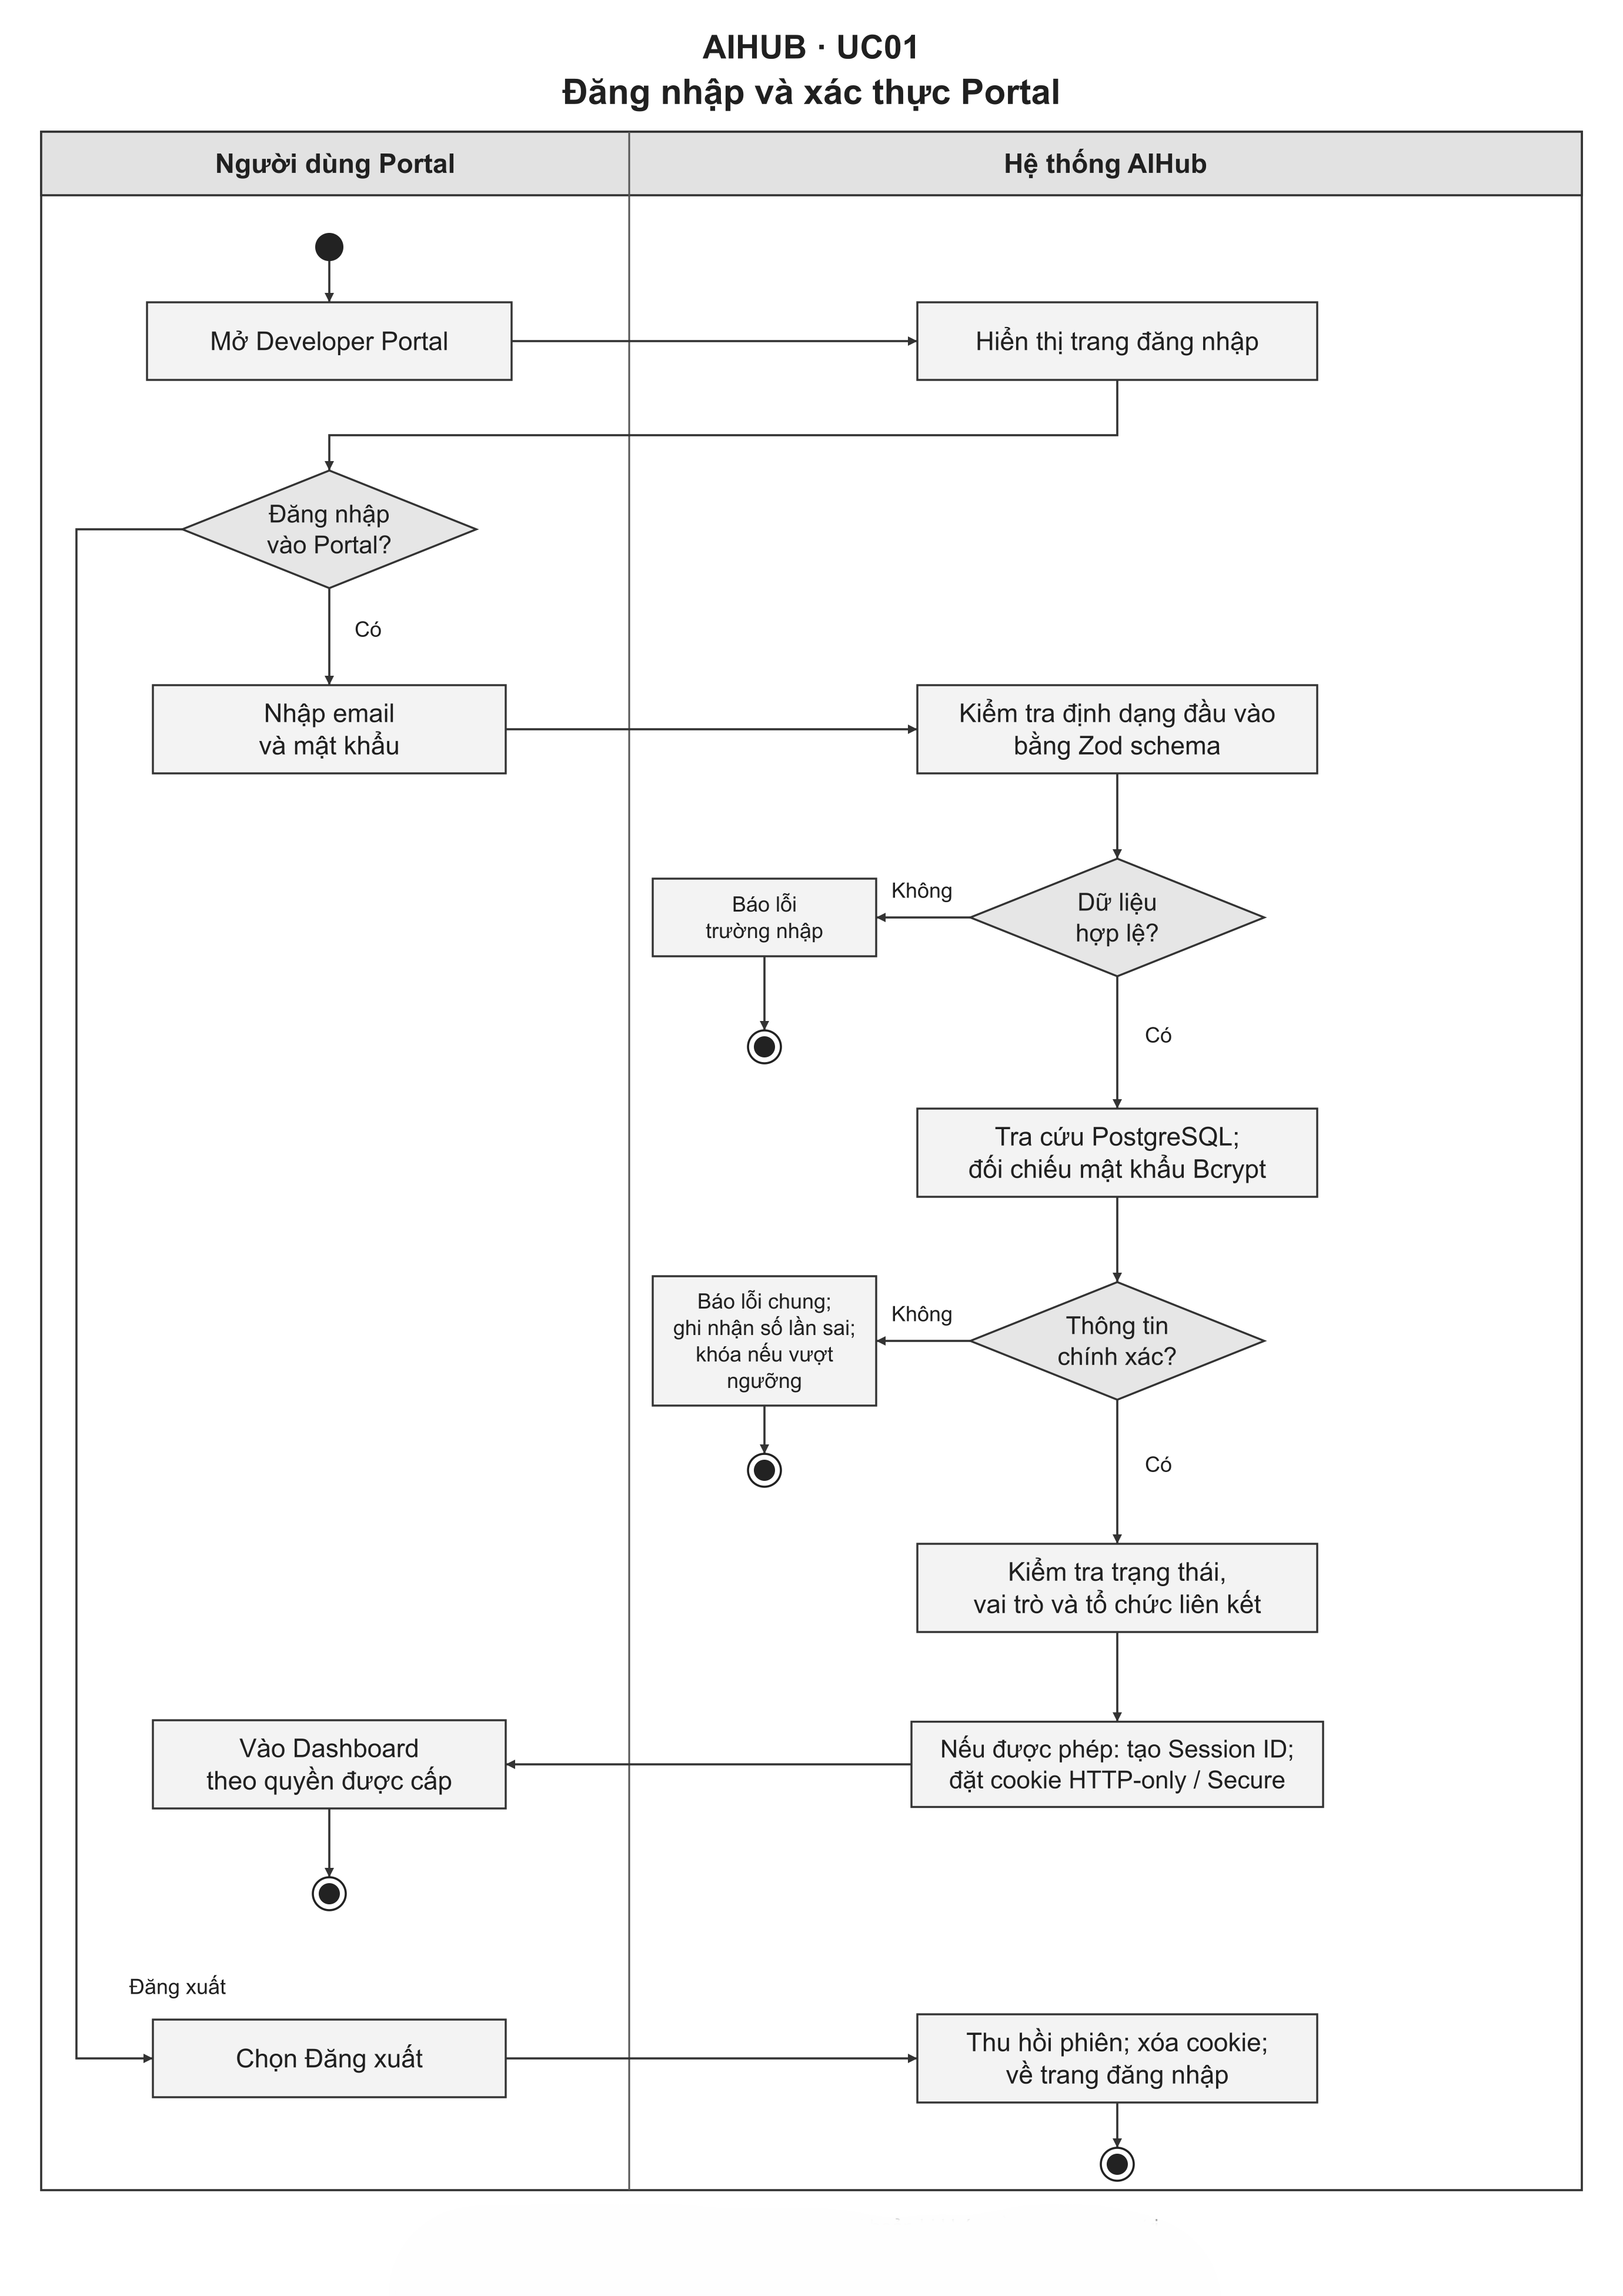
\includegraphics[width=\linewidth,height=0.72\textheight,keepaspectratio]{Images/Activity/AIHub/activity_uc01_portal_auth.png}
    \caption{Sơ đồ hoạt động AIHub -- Use-case 1: Đăng nhập và xác thực Portal}
    \label{aihub:fig:activity_uc01}
    \label{aihub:fig:act_uc1_dev_auth}
\end{figure}

Người dùng mở Portal và nhập thông tin đăng nhập. Khi đăng xuất, hệ thống thu hồi phiên và trở về trang đăng nhập.
% activity-generated:end


\clearpage

\paragraph{Luồng hoạt động: Quản lý khóa API (Use-case 2)}

% activity-generated:start
\begin{figure}[H]
    \centering
    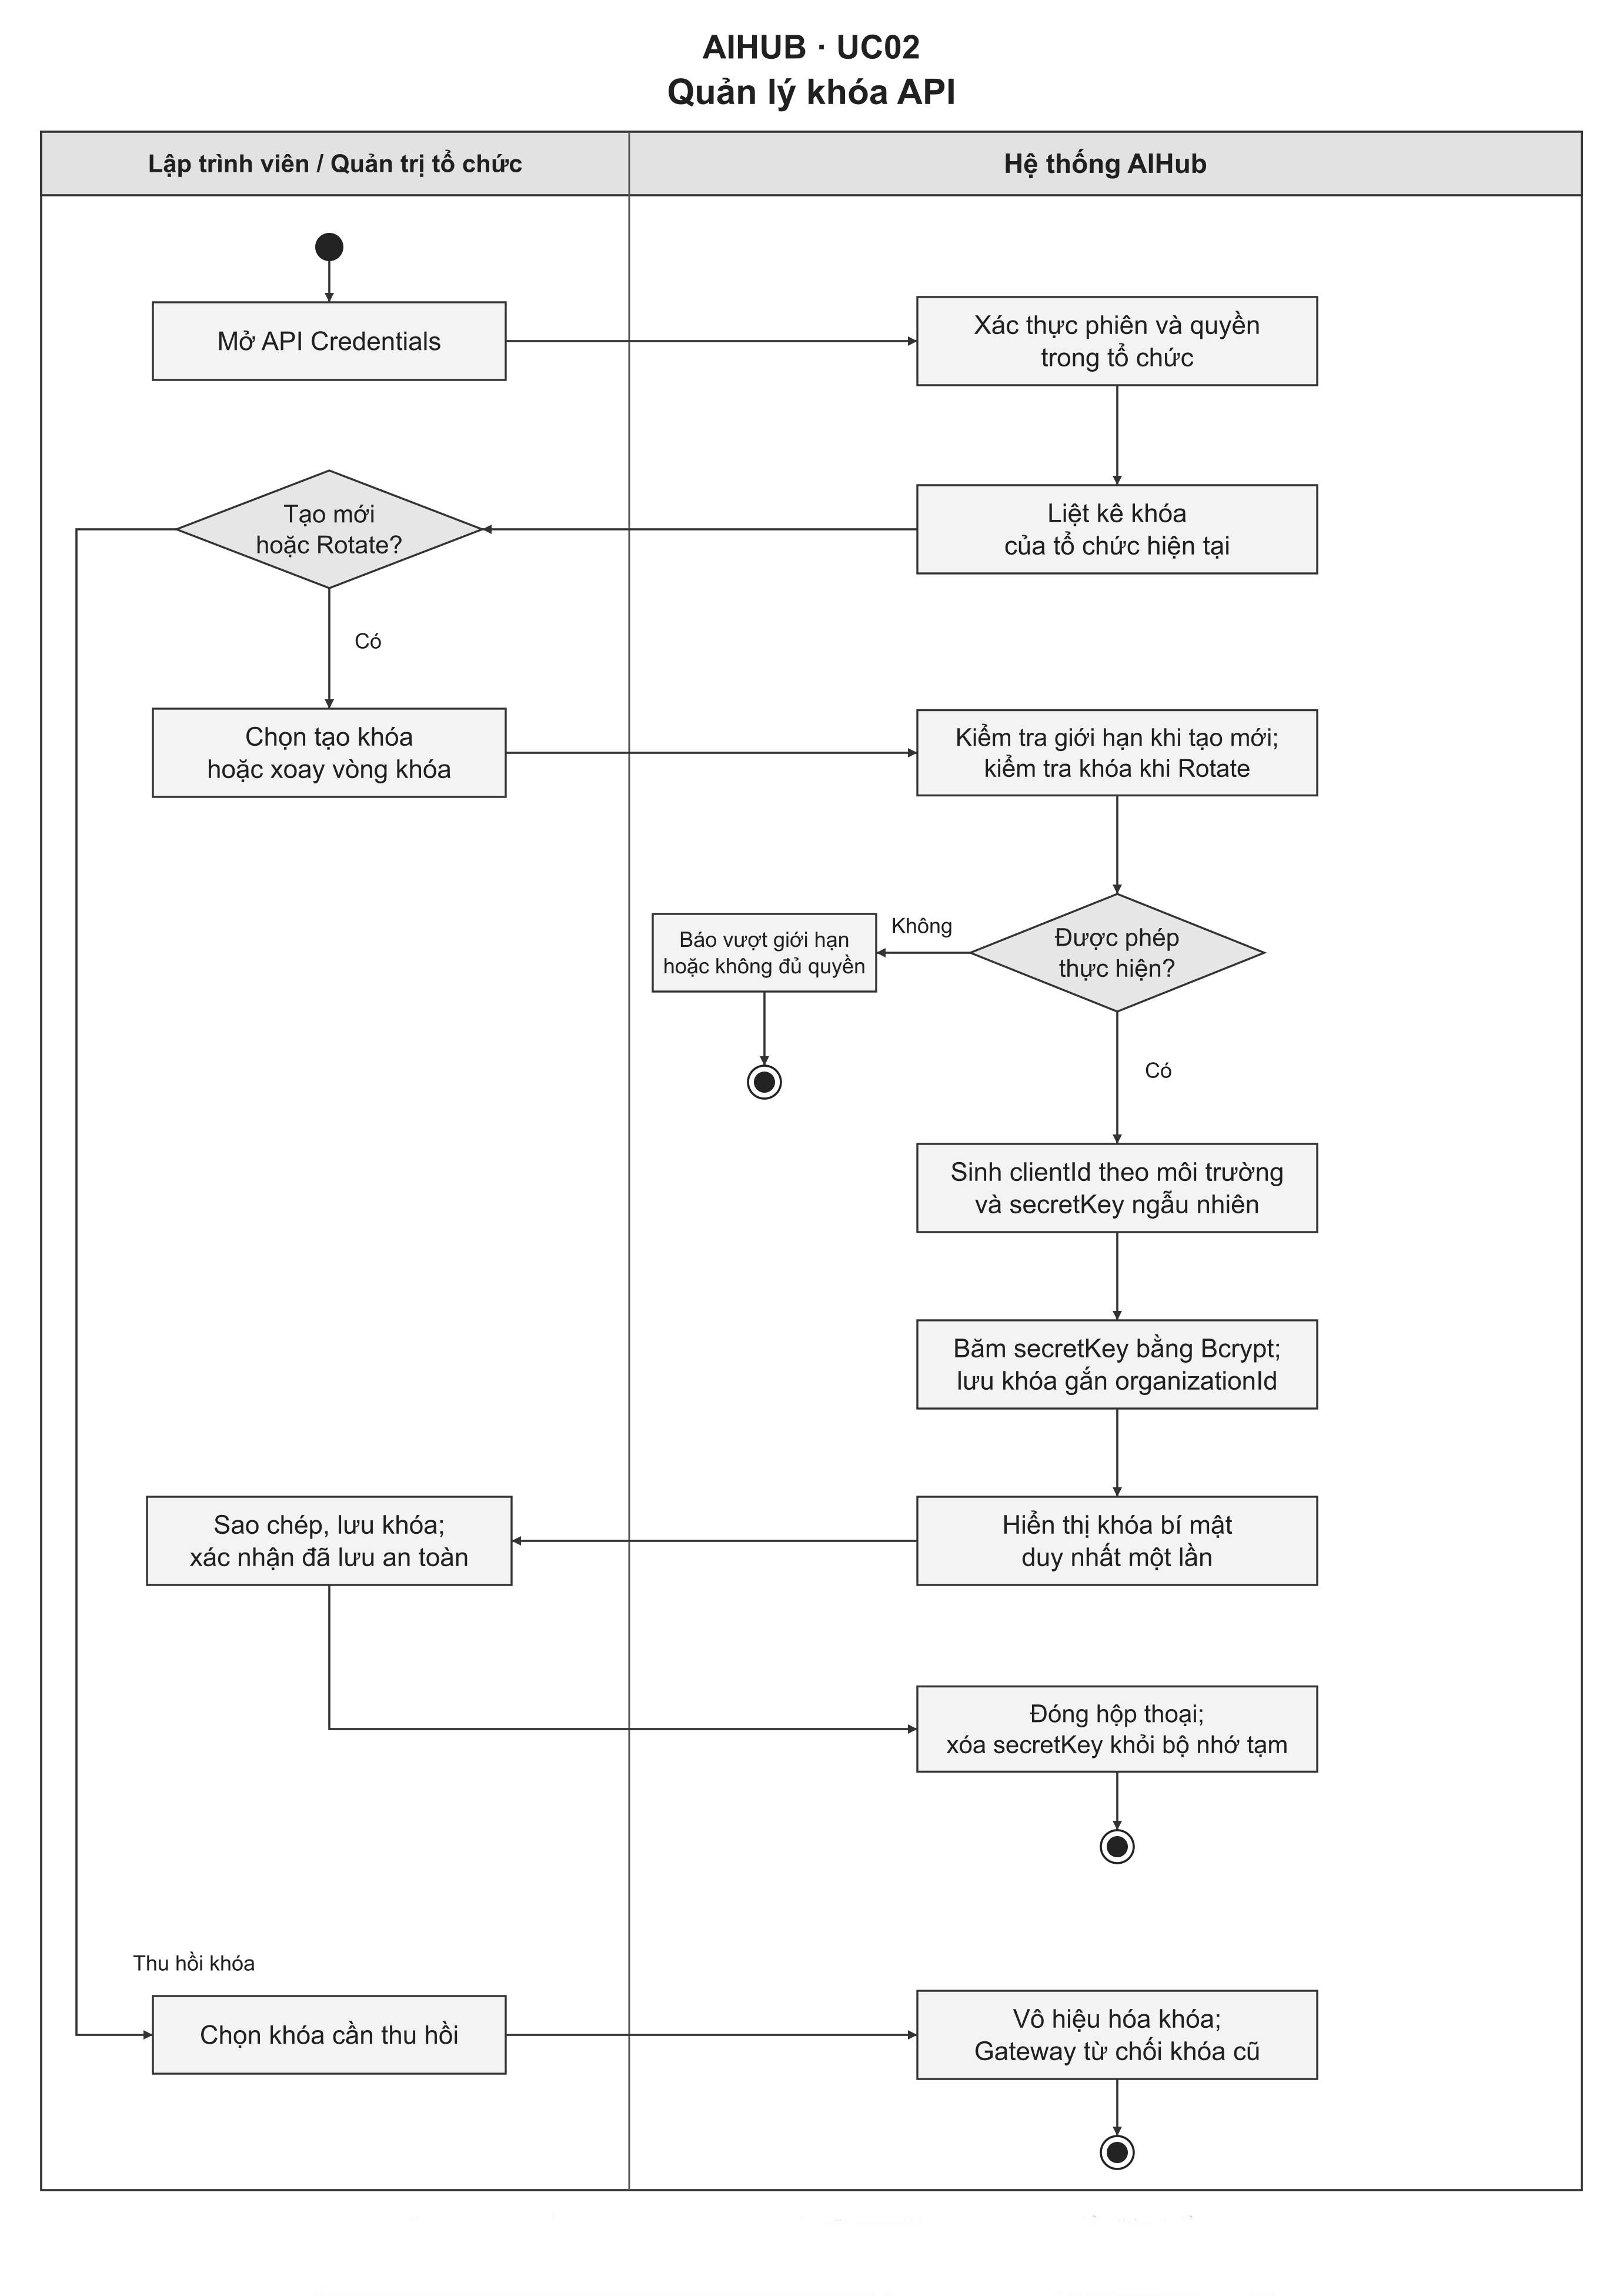
\includegraphics[width=\linewidth,height=0.72\textheight,keepaspectratio]{Images/Activity/AIHub/activity_uc02_api_credentials.png}
    \caption{Sơ đồ hoạt động AIHub -- Use-case 2: Quản lý khóa API}
    \label{aihub:fig:activity_uc02}
    \label{aihub:fig:act_uc2_manage_credentials}
\end{figure}

Người dùng mở danh sách khóa API và chọn tạo mới, xoay vòng hoặc thu hồi. Khóa bị thu hồi không còn được Gateway chấp nhận.
% activity-generated:end


\clearpage

\paragraph{Luồng hoạt động: Kiểm thử cURL Sandbox (Use-case 3)}

% activity-generated:start
\begin{figure}[H]
    \centering
    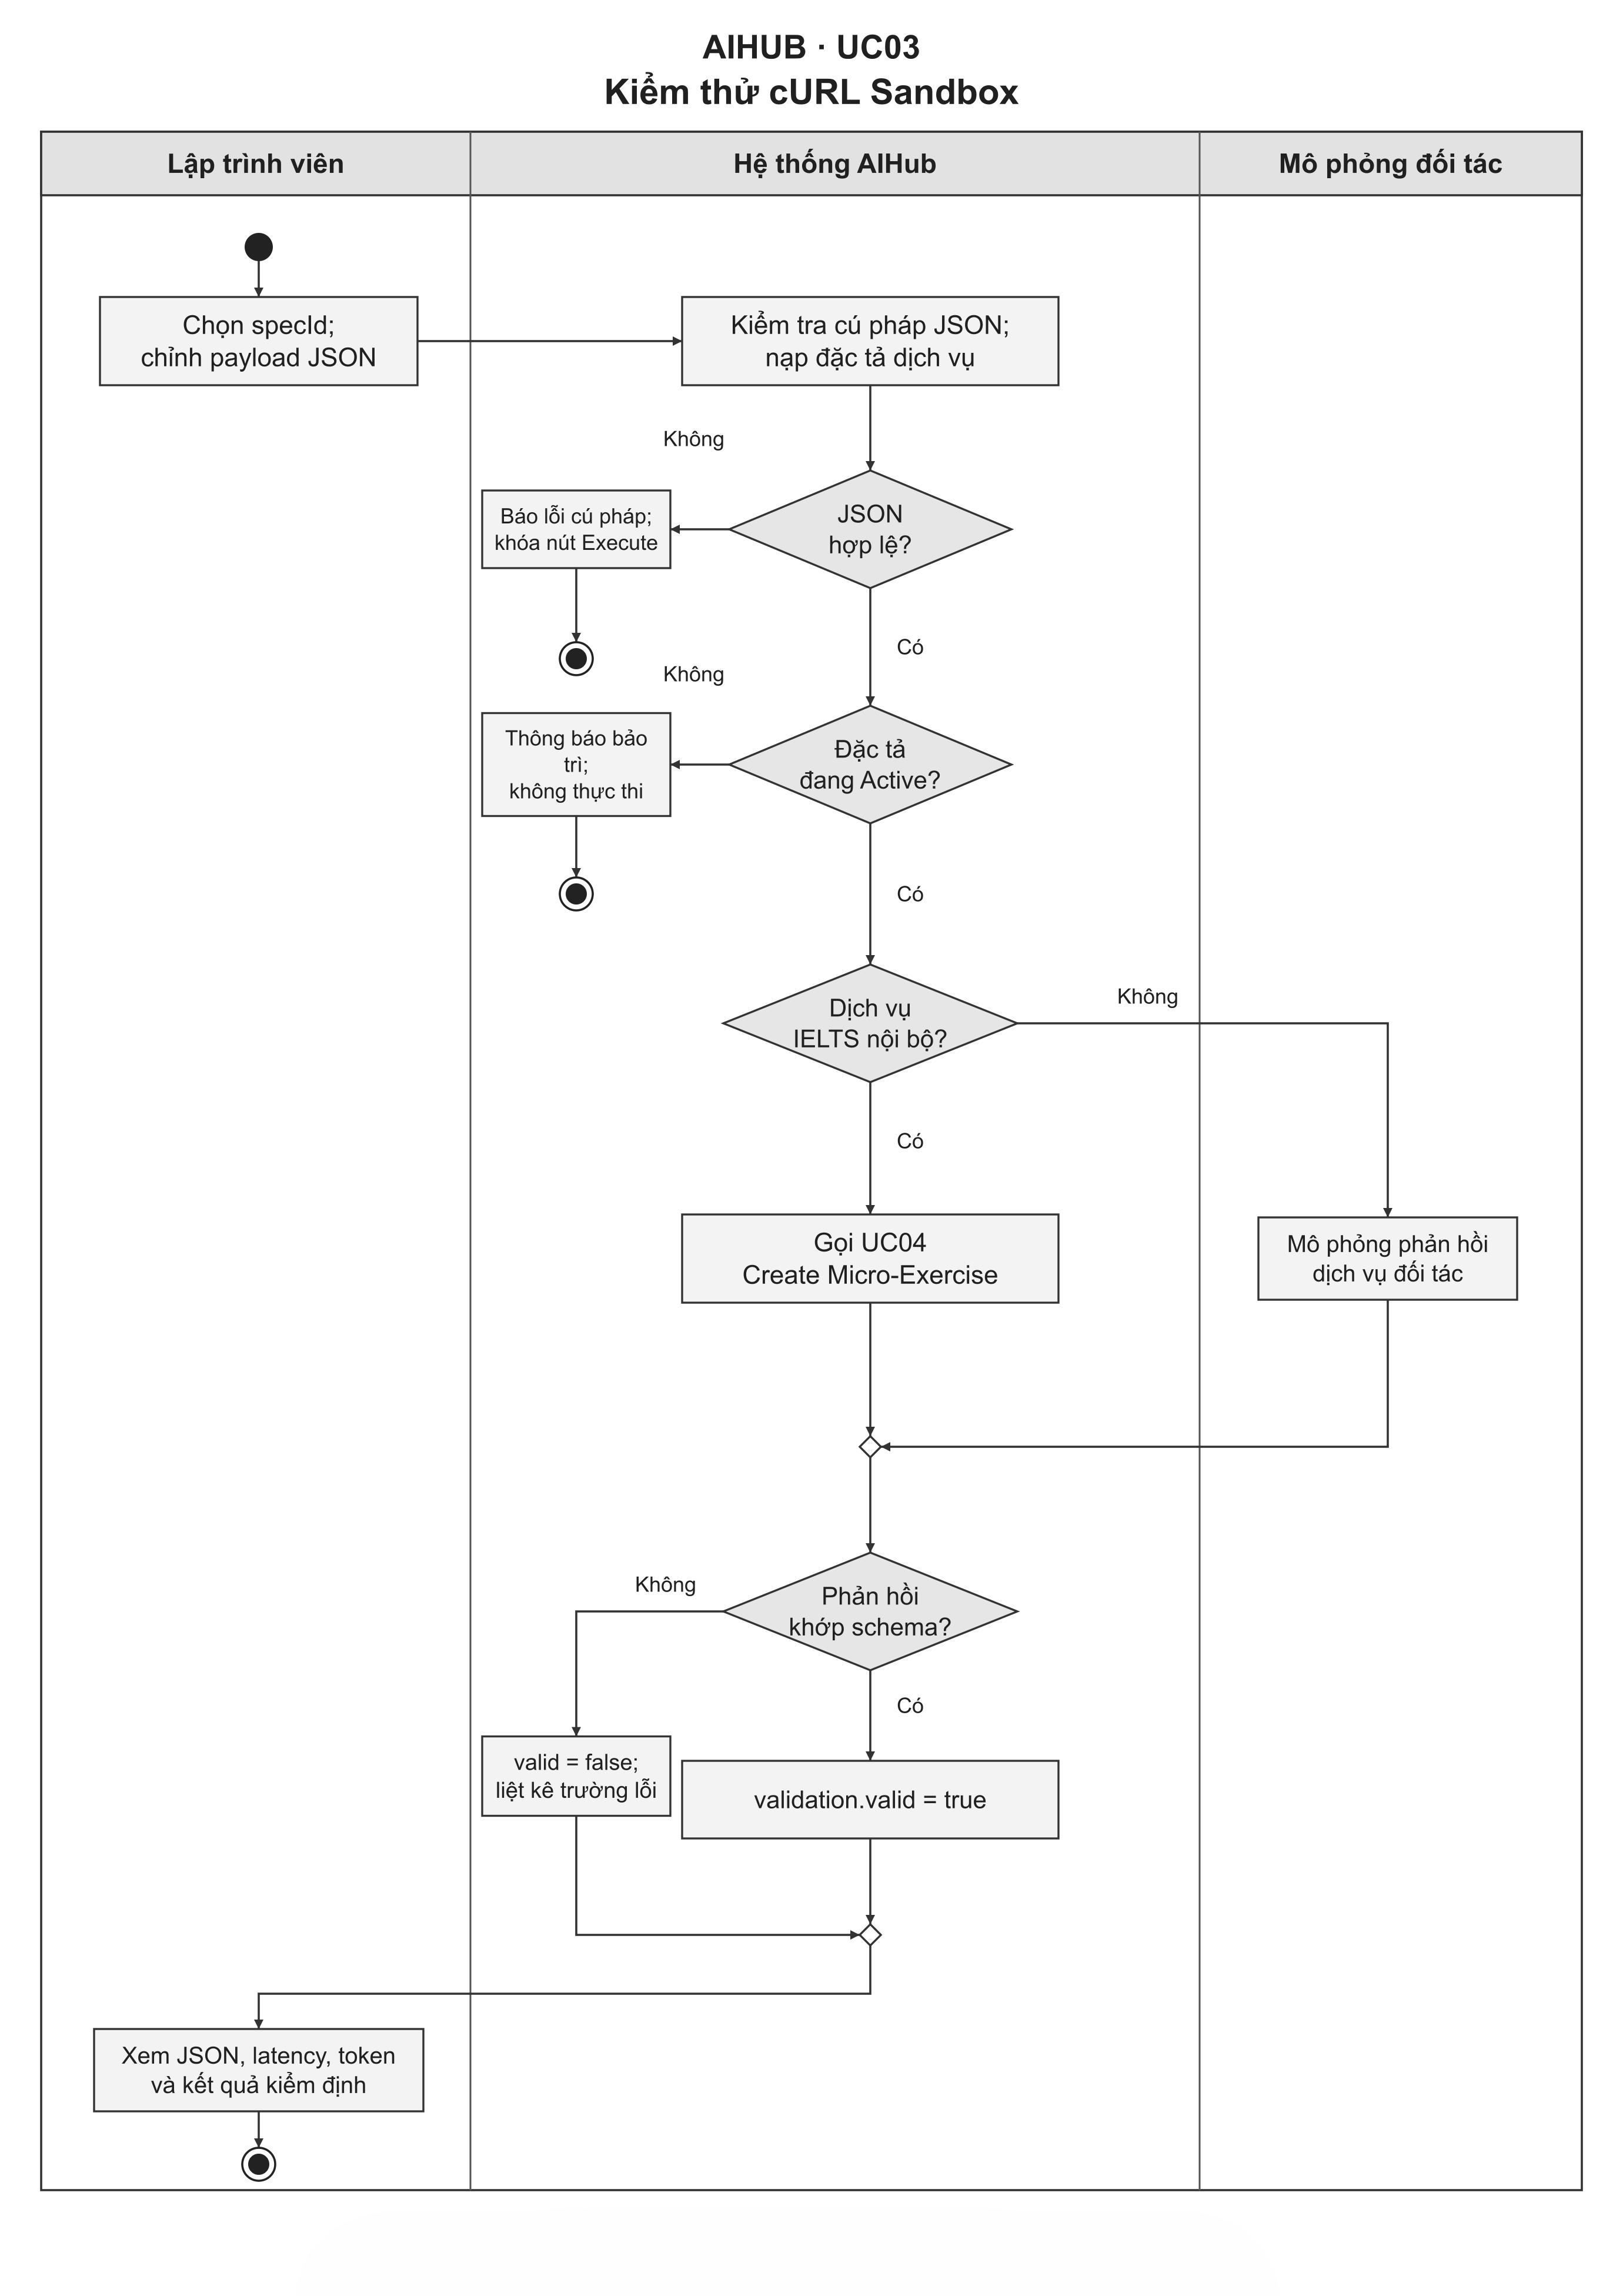
\includegraphics[width=\linewidth,height=0.72\textheight,keepaspectratio]{Images/Activity/AIHub/activity_uc03_curl_sandbox.png}
    \caption{Sơ đồ hoạt động AIHub -- Use-case 3: Kiểm thử cURL Sandbox}
    \label{aihub:fig:activity_uc03}
    \label{aihub:fig:act_uc3_run_spec_curl}
\end{figure}

Lập trình viên chọn đặc tả và nhập dữ liệu thử nghiệm. Sandbox hiển thị kết quả, thời gian xử lý và kết quả kiểm định.
% activity-generated:end


\clearpage

\paragraph{Luồng hoạt động: Gọi API sinh bài tập vi mô (Use-case 4)}

% activity-generated:start
\begin{figure}[H]
    \centering
    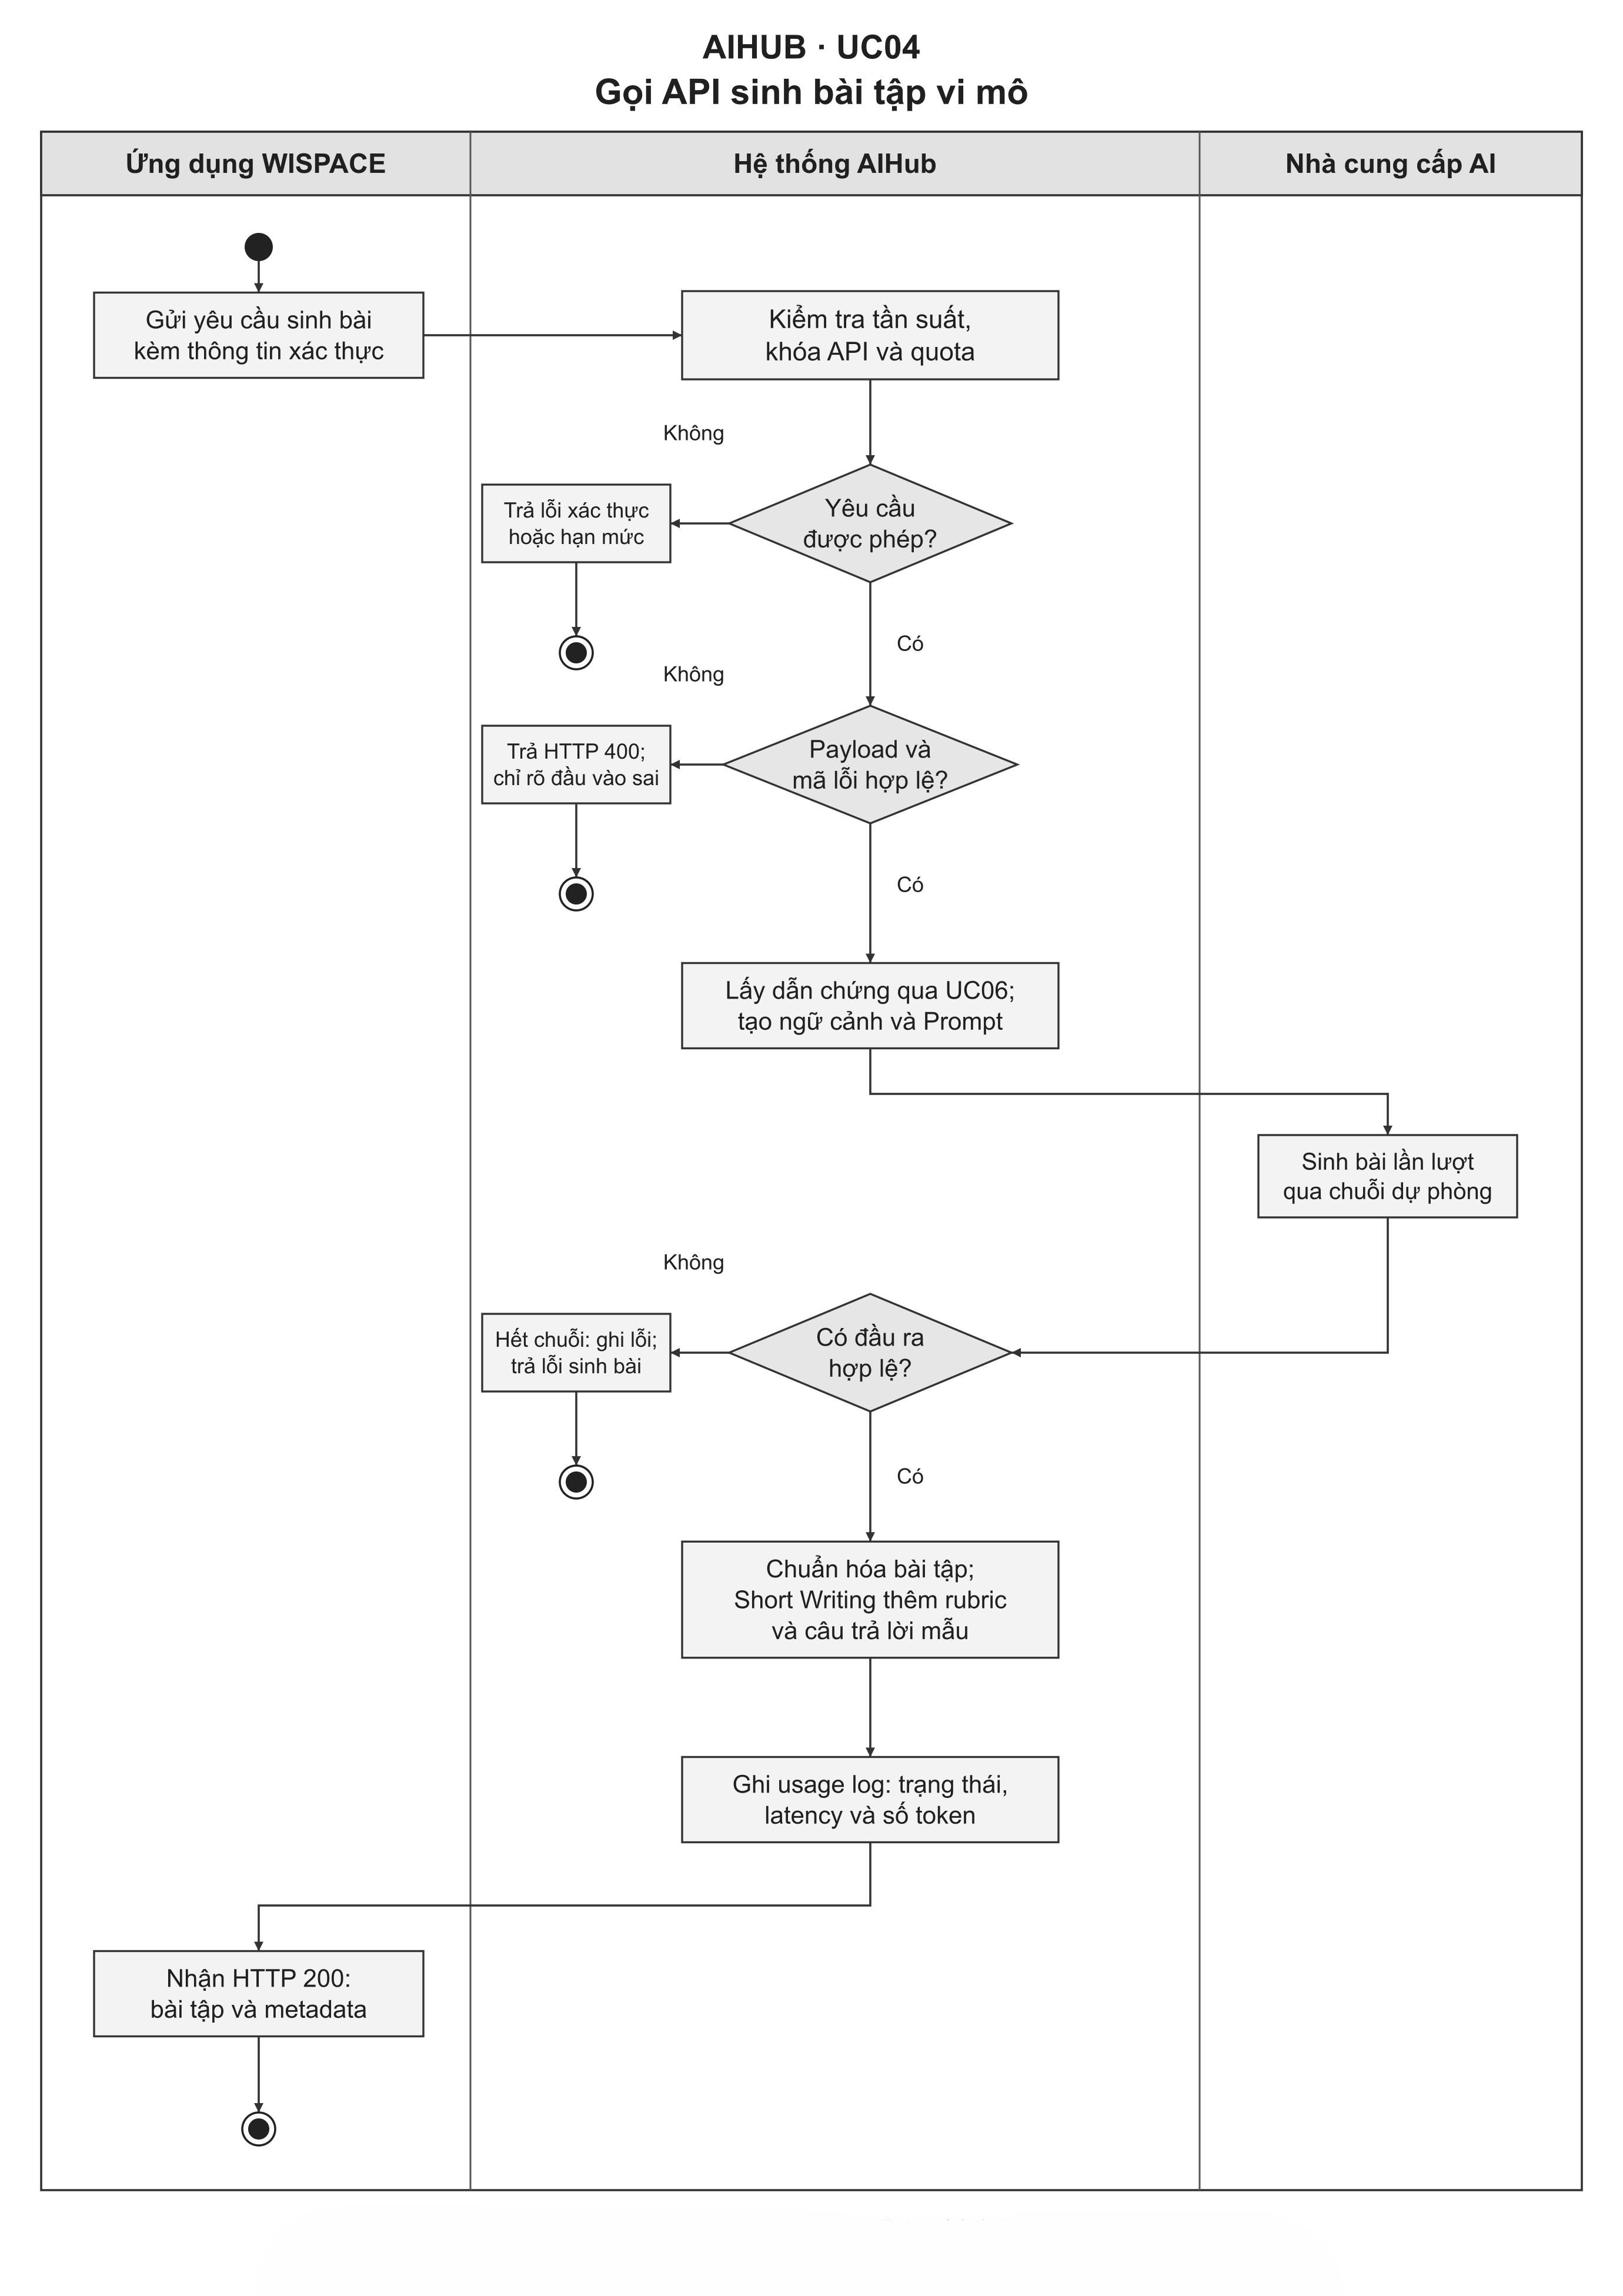
\includegraphics[width=\linewidth,height=0.72\textheight,keepaspectratio]{Images/Activity/AIHub/activity_uc04_create_micro_exercise.png}
    \caption{Sơ đồ hoạt động AIHub -- Use-case 4: Gọi API sinh bài tập vi mô}
    \label{aihub:fig:activity_uc04}
    \label{aihub:fig:act_uc4_create_micro_exercise}
\end{figure}

Ứng dụng gửi yêu cầu sinh bài tập kèm thông tin xác thực. Đầu ra hợp lệ được trả về và ghi nhật ký; nếu không thành công thì trả lỗi.
% activity-generated:end


\clearpage

\paragraph{Luồng hoạt động: Tra cứu hạn mức và Nhật ký sử dụng (Use-case 5)}

% activity-generated:start
\begin{figure}[H]
    \centering
    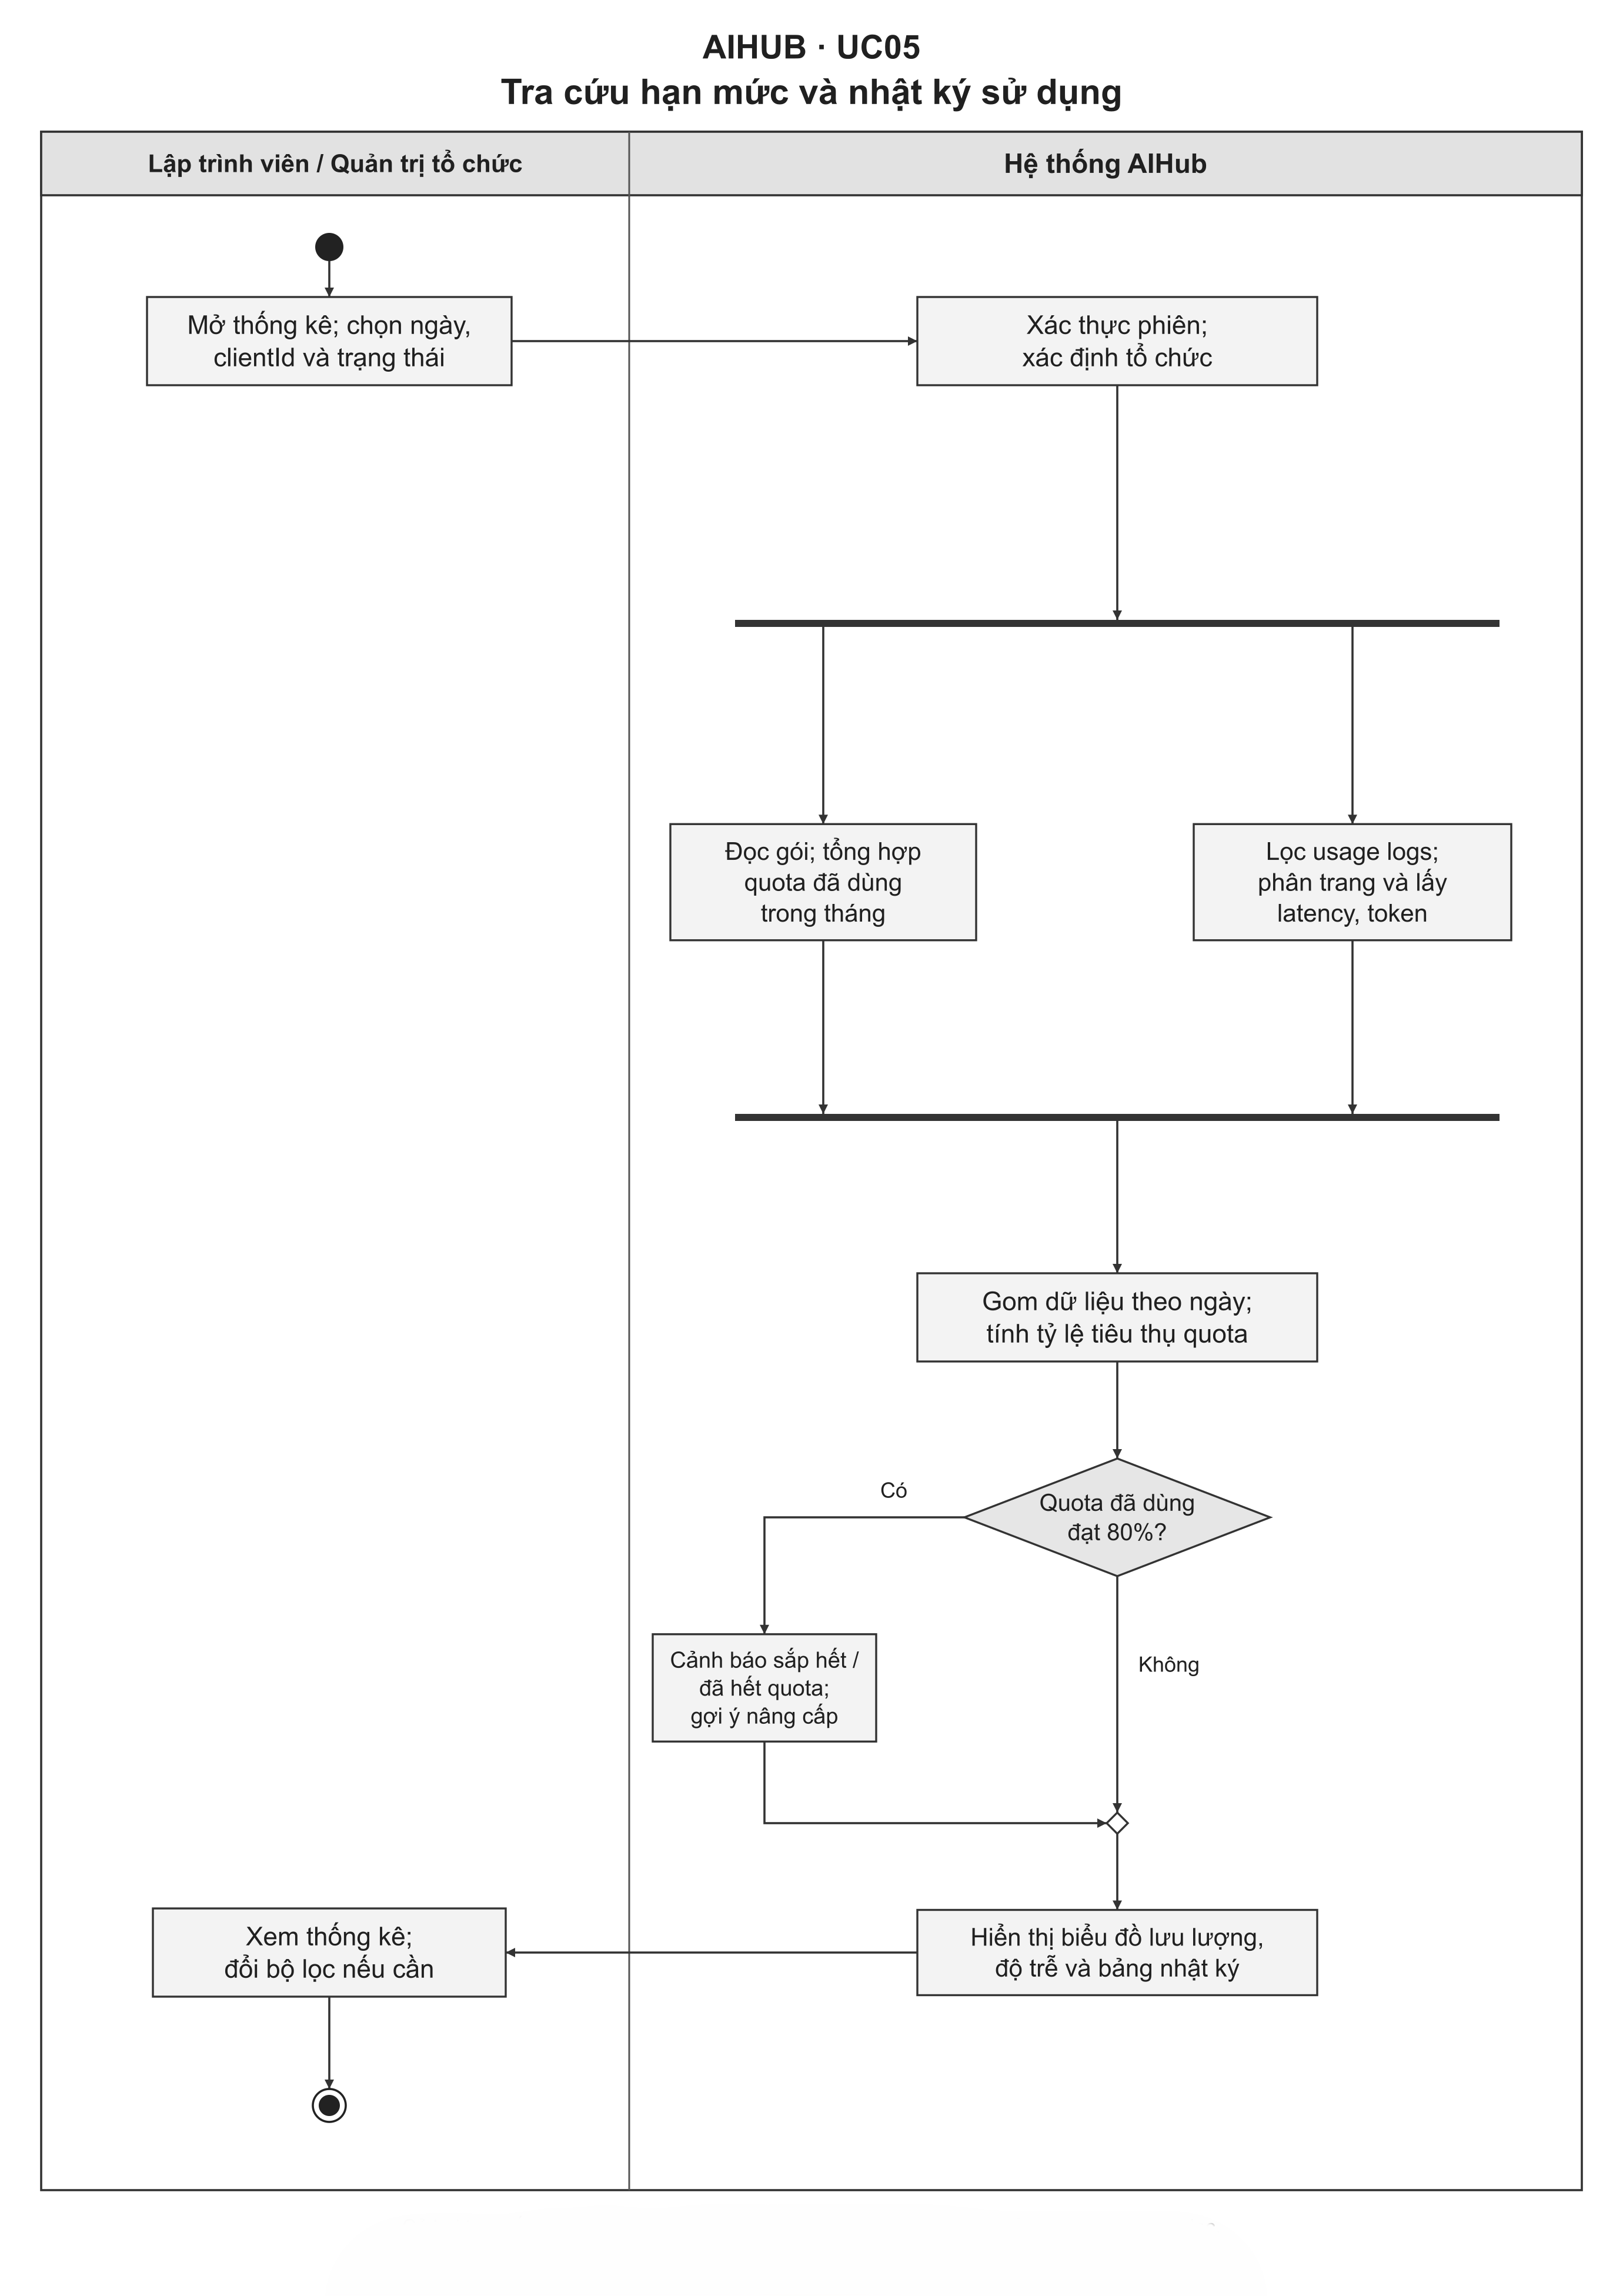
\includegraphics[width=\linewidth,height=0.72\textheight,keepaspectratio]{Images/Activity/AIHub/activity_uc05_quota_usage_logs.png}
    \caption{Sơ đồ hoạt động AIHub -- Use-case 5: Tra cứu hạn mức và nhật ký sử dụng}
    \label{aihub:fig:activity_uc05}
    \label{aihub:fig:act_uc5_view_usage_logs}
\end{figure}

Người dùng chọn khoảng thời gian và điều kiện tra cứu. Kết quả được tổng hợp để hiển thị, xem chi tiết hoặc xuất dữ liệu.
% activity-generated:end


% =========================================================================
% NHÓM 2: CHUYÊN VIÊN HỌC THUẬT (USE-CASE 6 - 11)
% =========================================================================

\clearpage

\paragraph{Luồng hoạt động: Truy vấn ngân hàng lỗi thực tế (Use-case 6)}

% activity-generated:start
\begin{figure}[H]
    \centering
    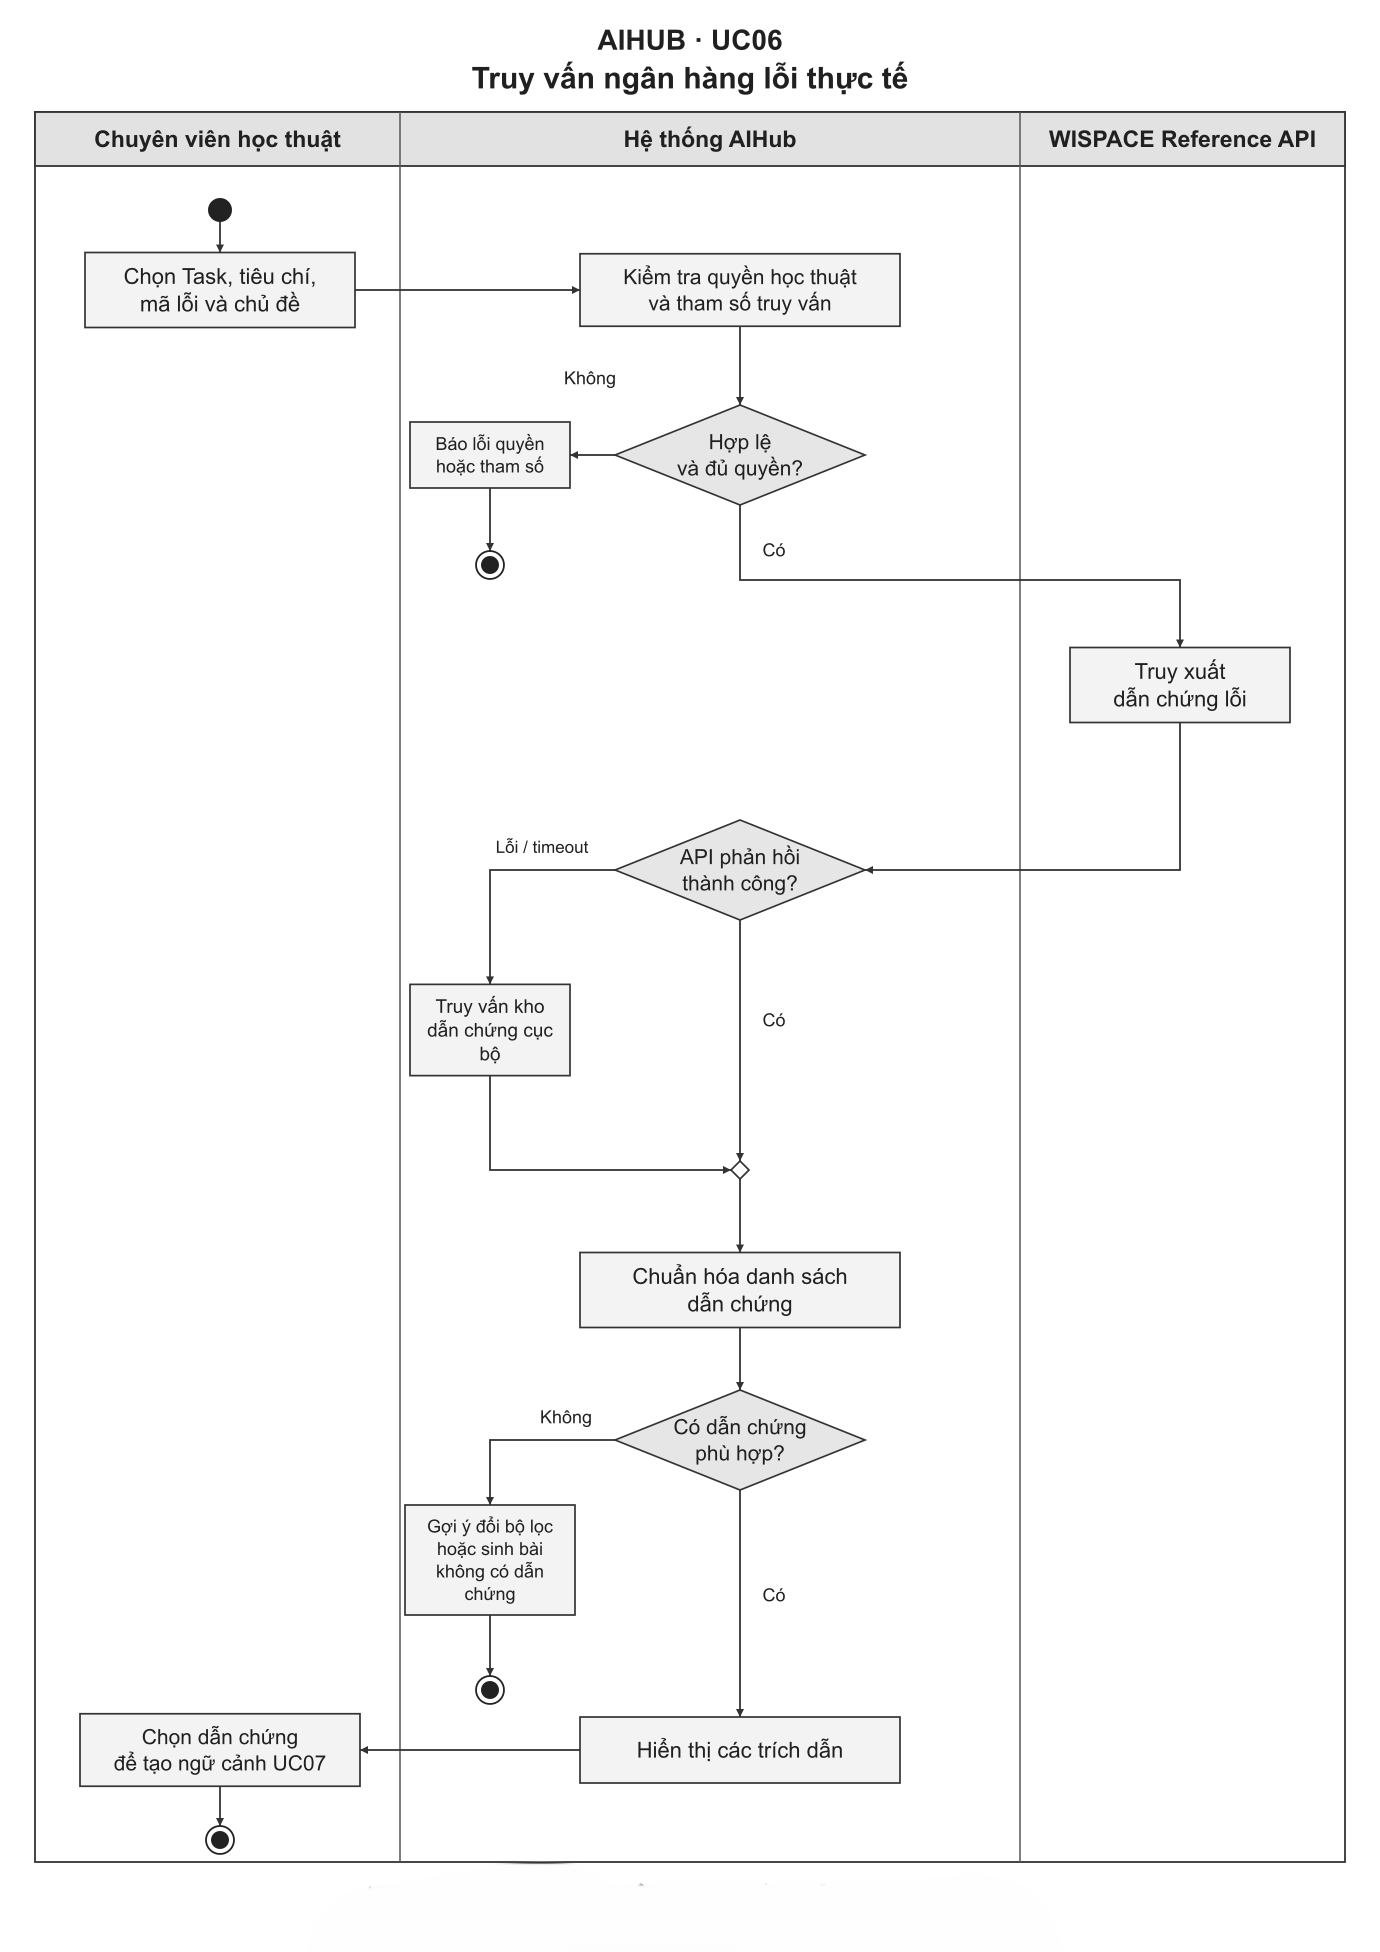
\includegraphics[width=\linewidth,height=0.72\textheight,keepaspectratio]{Images/Activity/AIHub/activity_uc06_essay_references.png}
    \caption{Sơ đồ hoạt động AIHub -- Use-case 6: Truy vấn ngân hàng lỗi thực tế}
    \label{aihub:fig:activity_uc06}
    \label{aihub:fig:act_uc6_query_references}
\end{figure}

Chuyên viên chọn Task, tiêu chí, mã lỗi và chủ đề. Chuyên viên chọn dẫn chứng để tạo ngữ cảnh sinh bài.
% activity-generated:end


\clearpage

\paragraph{Luồng hoạt động: Khởi tạo mẫu bài tập học thuật (Use-case 7)}

% activity-generated:start
\begin{figure}[H]
    \centering
    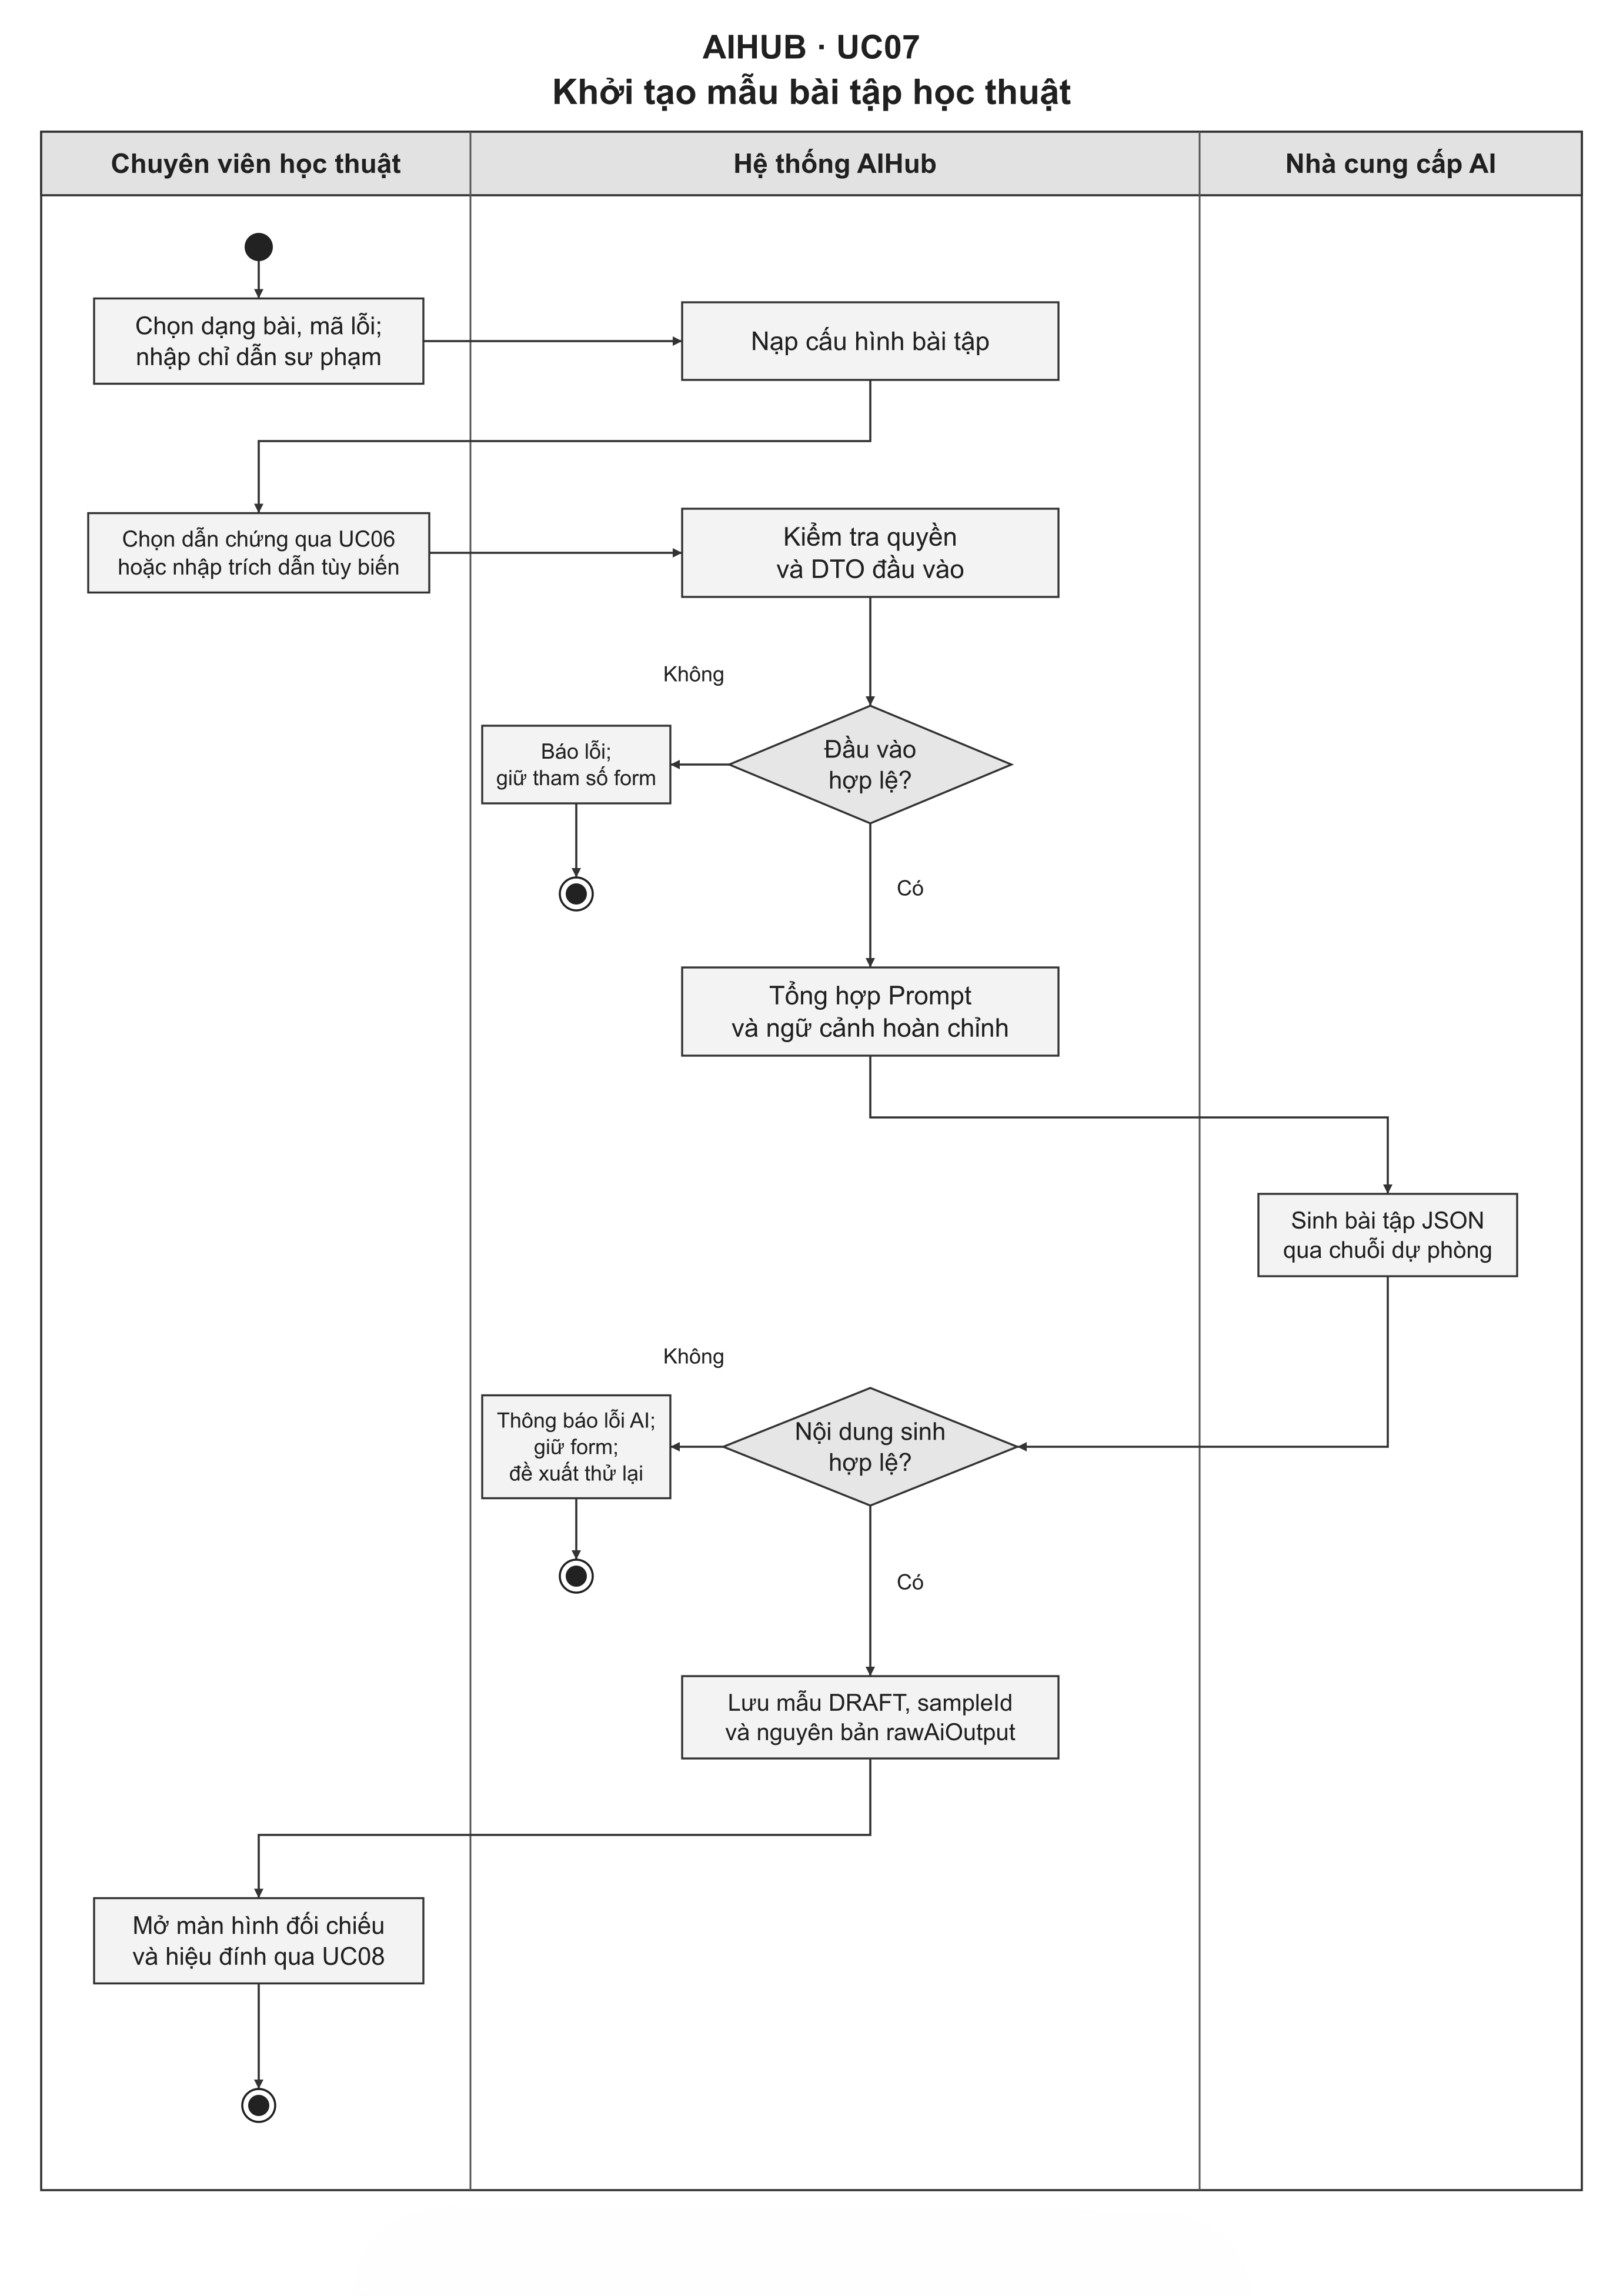
\includegraphics[width=\linewidth,height=0.72\textheight,keepaspectratio]{Images/Activity/AIHub/activity_uc07_generate_academic_sample.png}
    \caption{Sơ đồ hoạt động AIHub -- Use-case 7: Khởi tạo mẫu bài tập học thuật}
    \label{aihub:fig:activity_uc07}
    \label{aihub:fig:act_uc7_academic_generate}
\end{figure}

Chuyên viên chọn yêu cầu bài tập và bổ sung ngữ cảnh hoặc dẫn chứng. Chuyên viên mở mẫu để hiệu đính; nếu sinh lỗi thì có thể thử lại.
% activity-generated:end


\clearpage

\paragraph{Luồng hoạt động: Kiểm định, hiệu đính và chấm điểm bài tập (Use-case 8)}

% activity-generated:start
\begin{figure}[H]
    \centering
    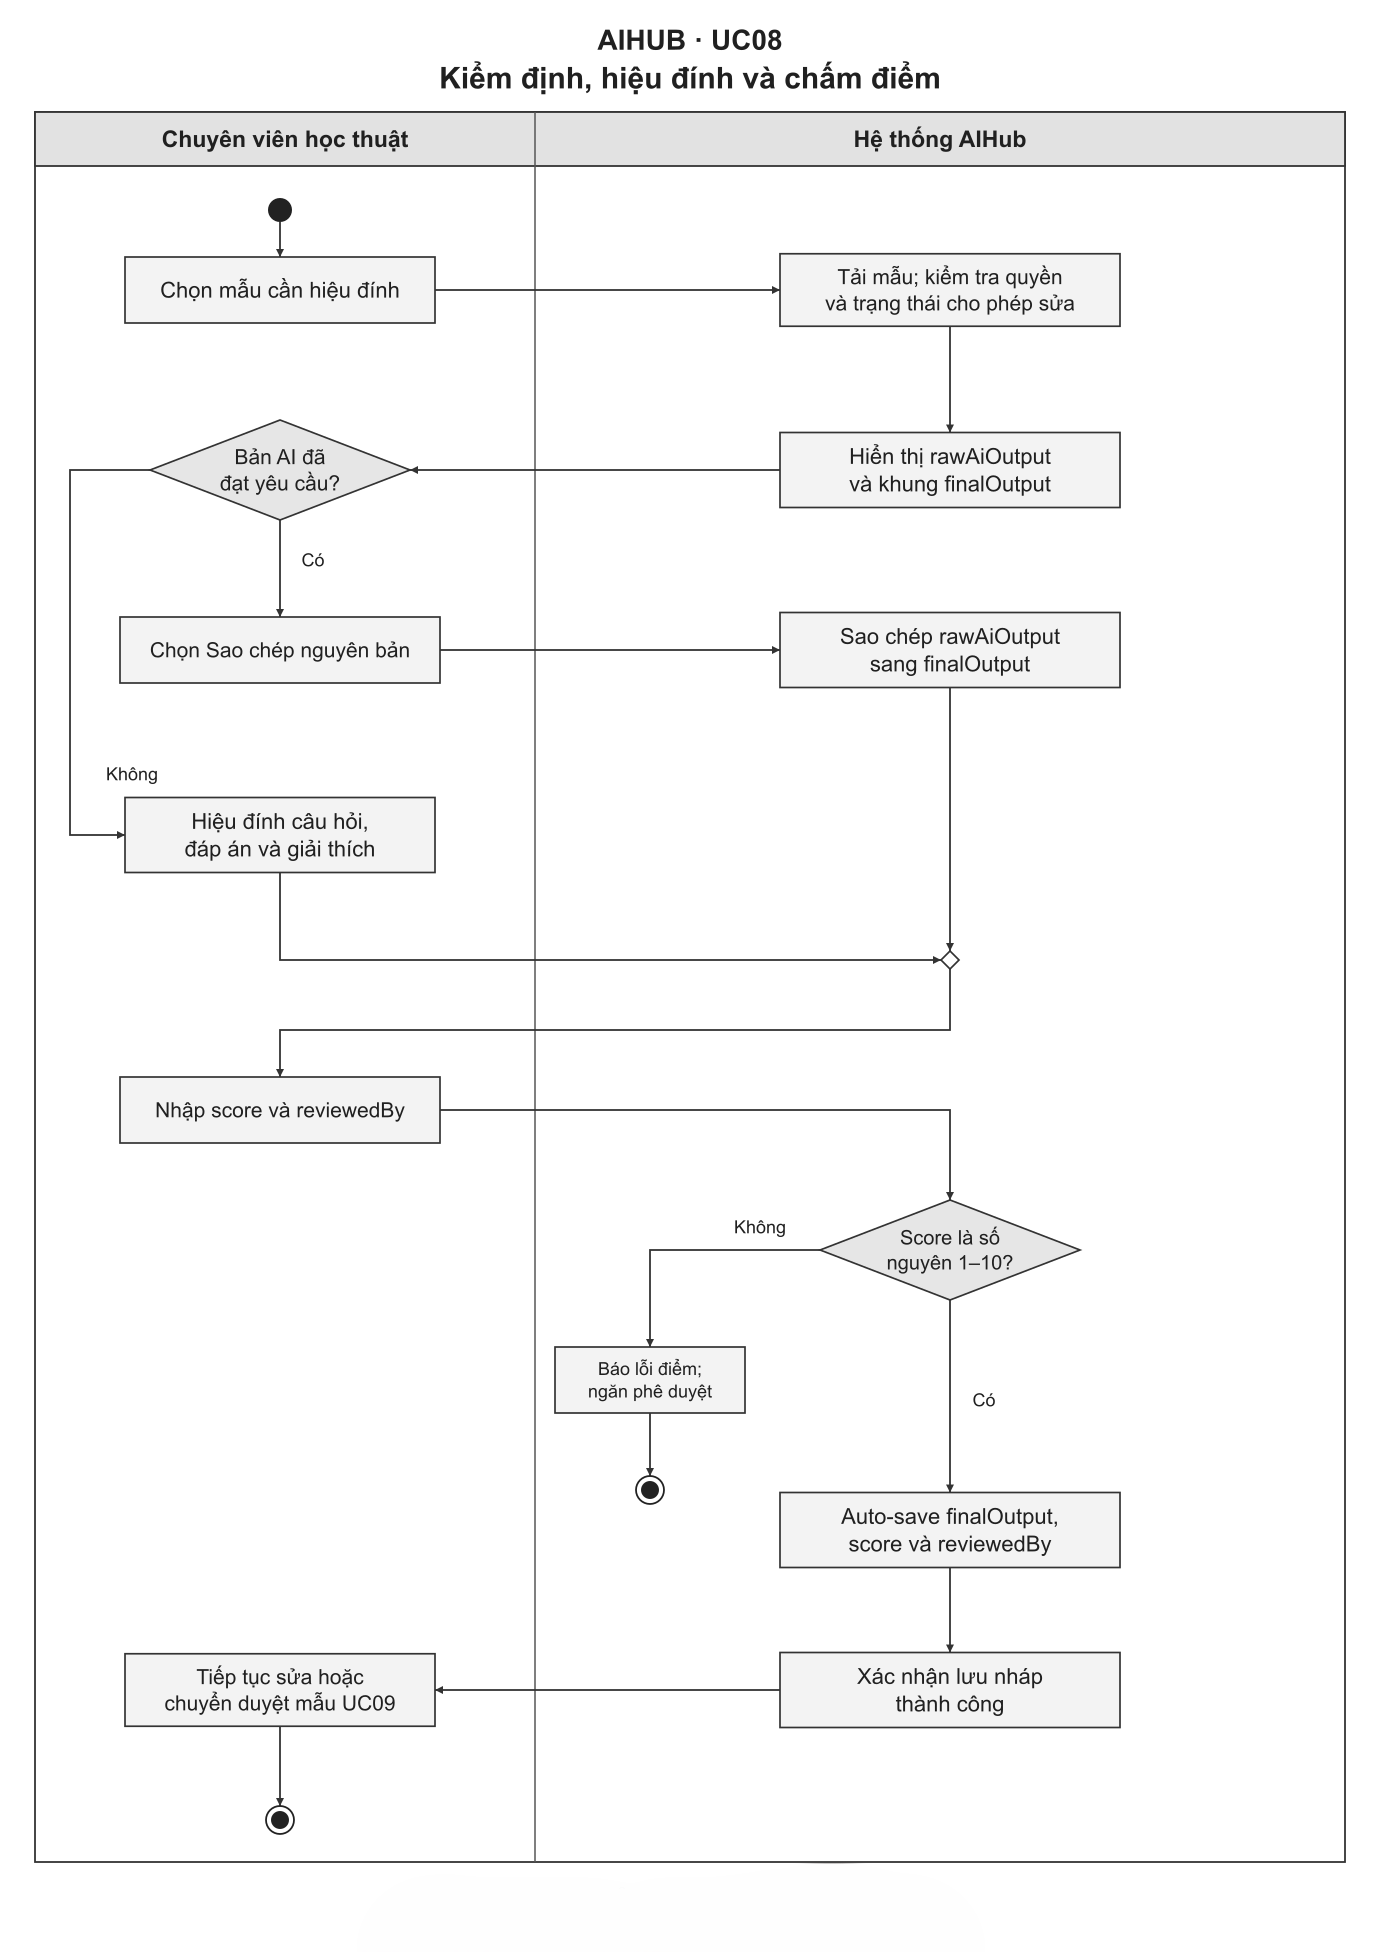
\includegraphics[width=\linewidth,height=0.72\textheight,keepaspectratio]{Images/Activity/AIHub/activity_uc08_review_score_sample.png}
    \caption{Sơ đồ hoạt động AIHub -- Use-case 8: Kiểm định, hiệu đính và chấm điểm}
    \label{aihub:fig:activity_uc08}
    \label{aihub:fig:act_uc8_academic_review_score}
\end{figure}

Chuyên viên mở mẫu và xem nội dung AI đã tạo. Chuyên viên tiếp tục chỉnh sửa hoặc chuyển sang duyệt mẫu.
% activity-generated:end


\clearpage

\paragraph{Luồng hoạt động: Chấp thuận mẫu và xoay vòng lỗi (Use-case 9)}

% activity-generated:start
\begin{figure}[H]
    \centering
    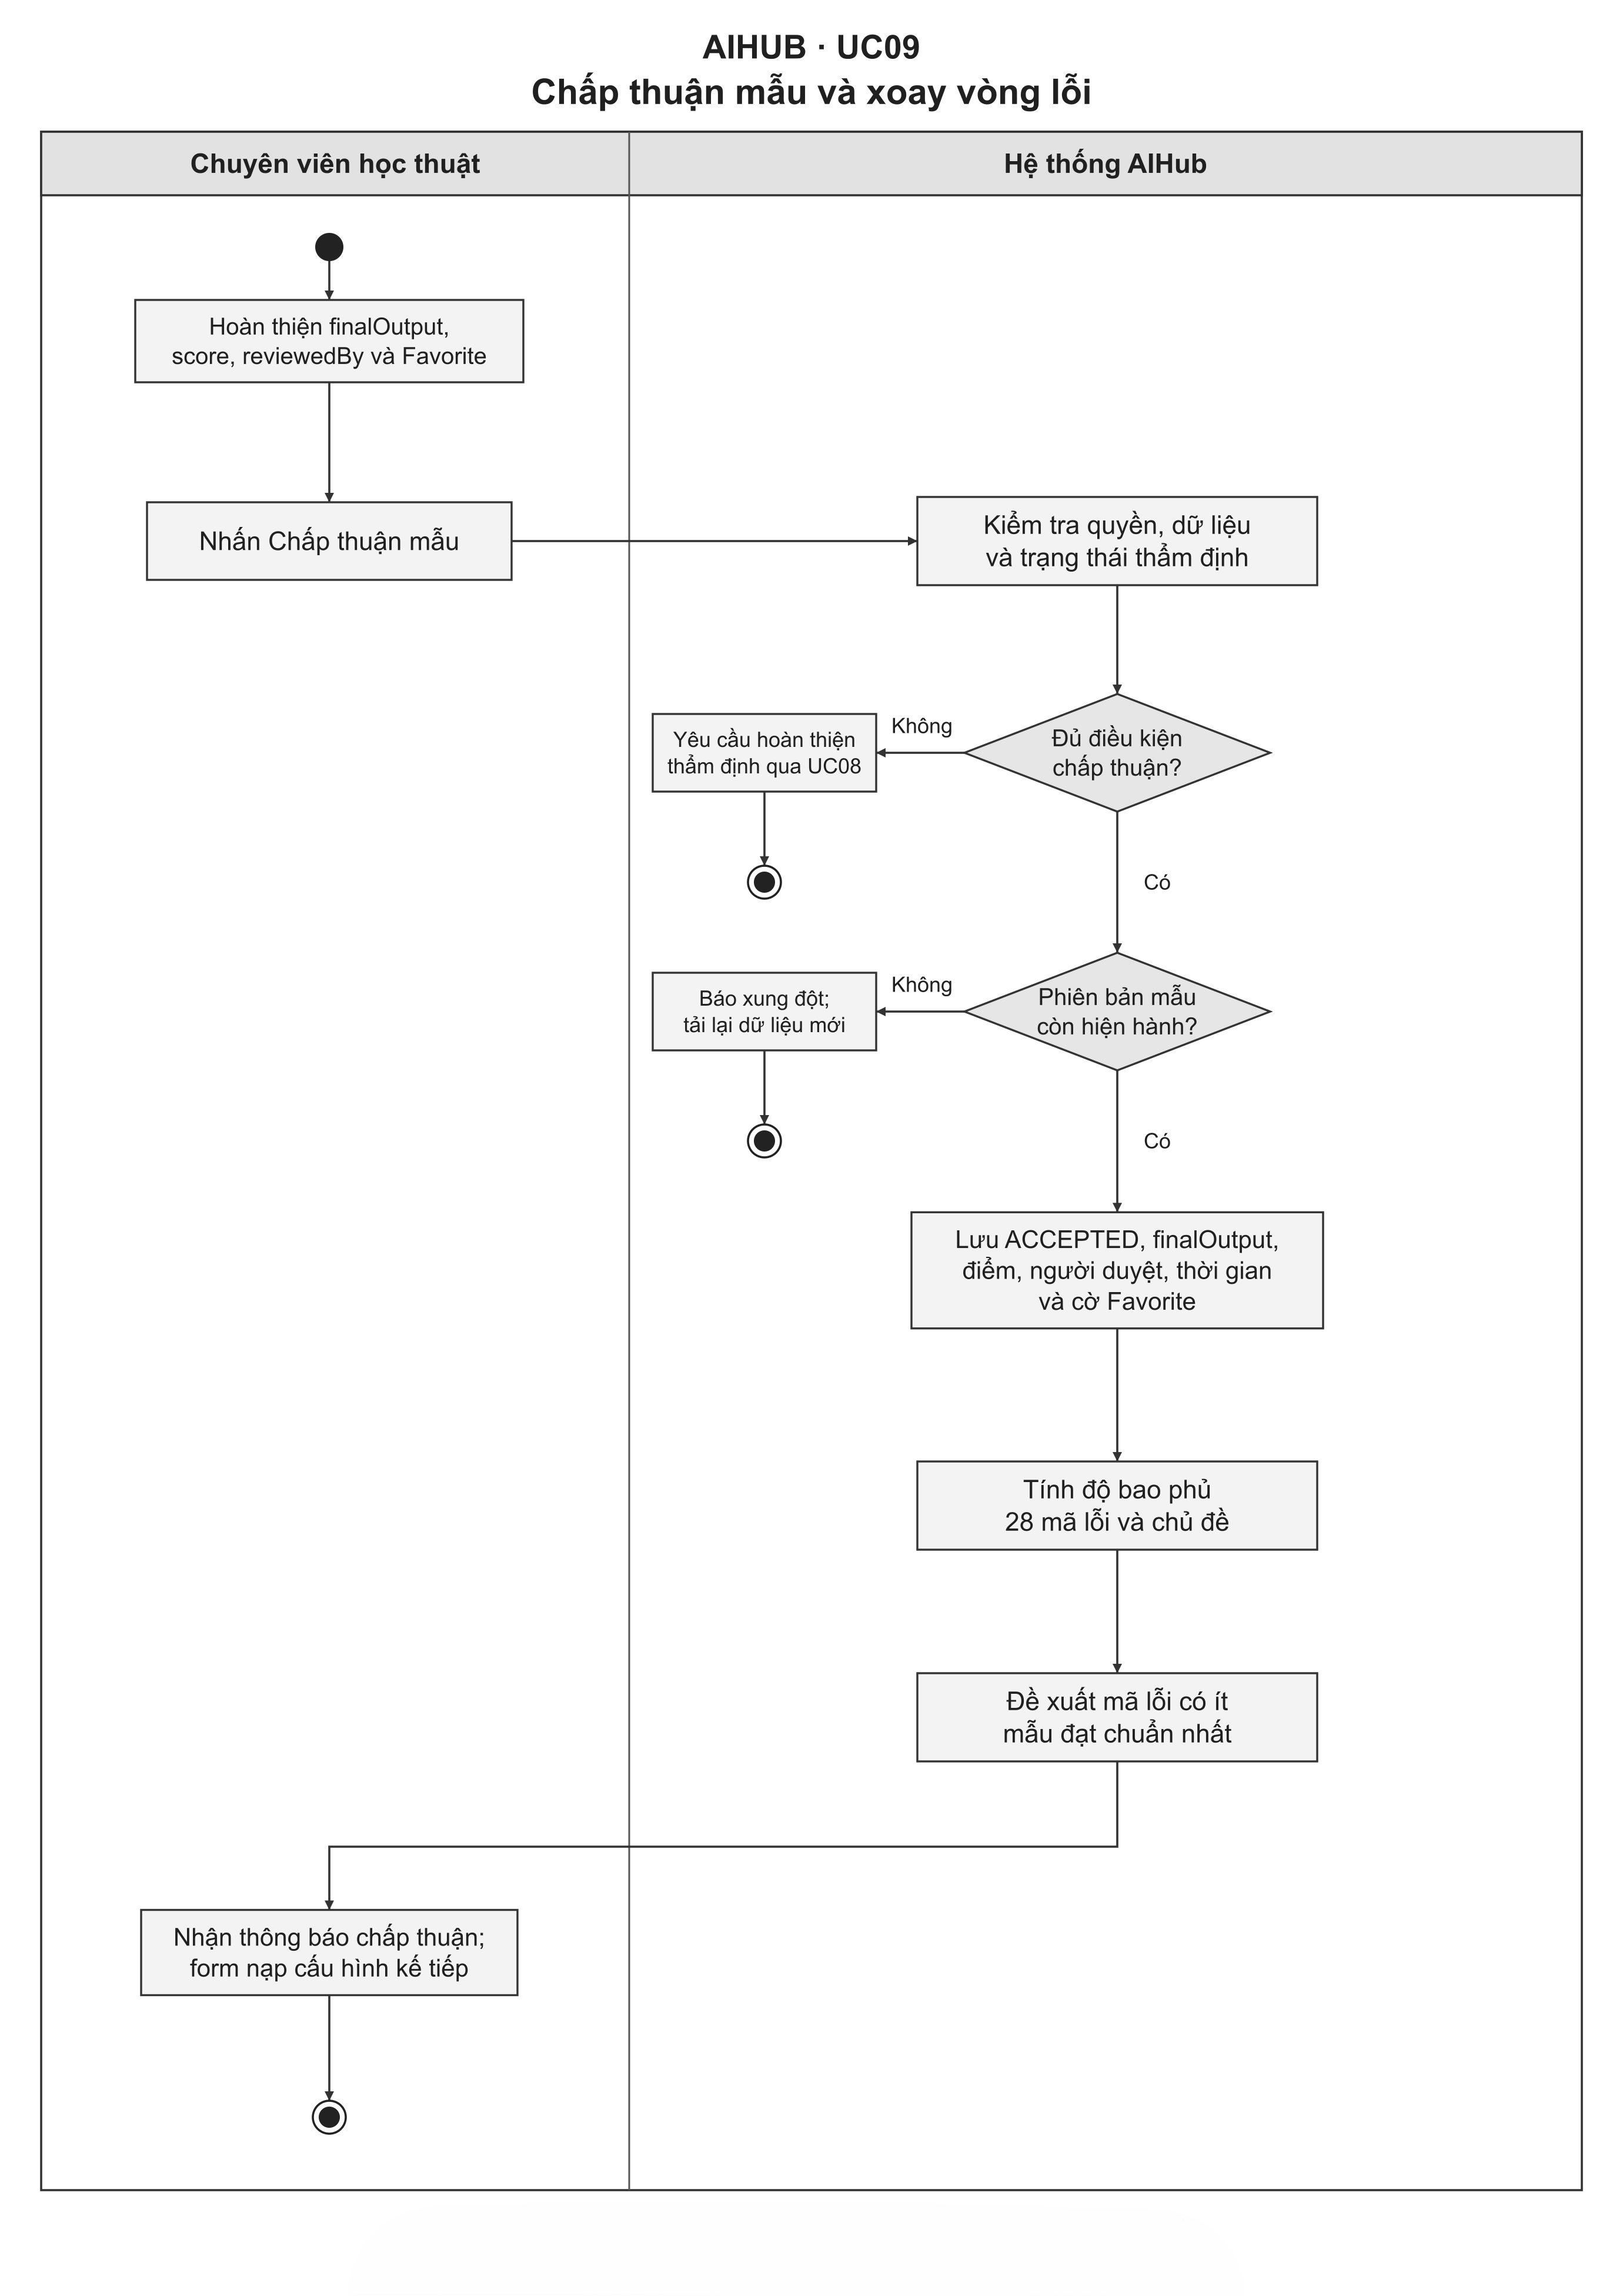
\includegraphics[width=\linewidth,height=0.72\textheight,keepaspectratio]{Images/Activity/AIHub/activity_uc09_accept_sample.png}
    \caption{Sơ đồ hoạt động AIHub -- Use-case 9: Chấp thuận mẫu và xoay vòng lỗi}
    \label{aihub:fig:activity_uc09}
    \label{aihub:fig:act_uc9_academic_accept}
\end{figure}

Chuyên viên kiểm tra mẫu và chọn chấp thuận. Hệ thống cập nhật mức bao phủ lỗi và gợi ý mẫu tiếp theo.
% activity-generated:end


\clearpage

\paragraph{Luồng hoạt động: Từ chối mẫu và thu thập dữ liệu tinh chỉnh (Use-case 10)}

% activity-generated:start
\begin{figure}[H]
    \centering
    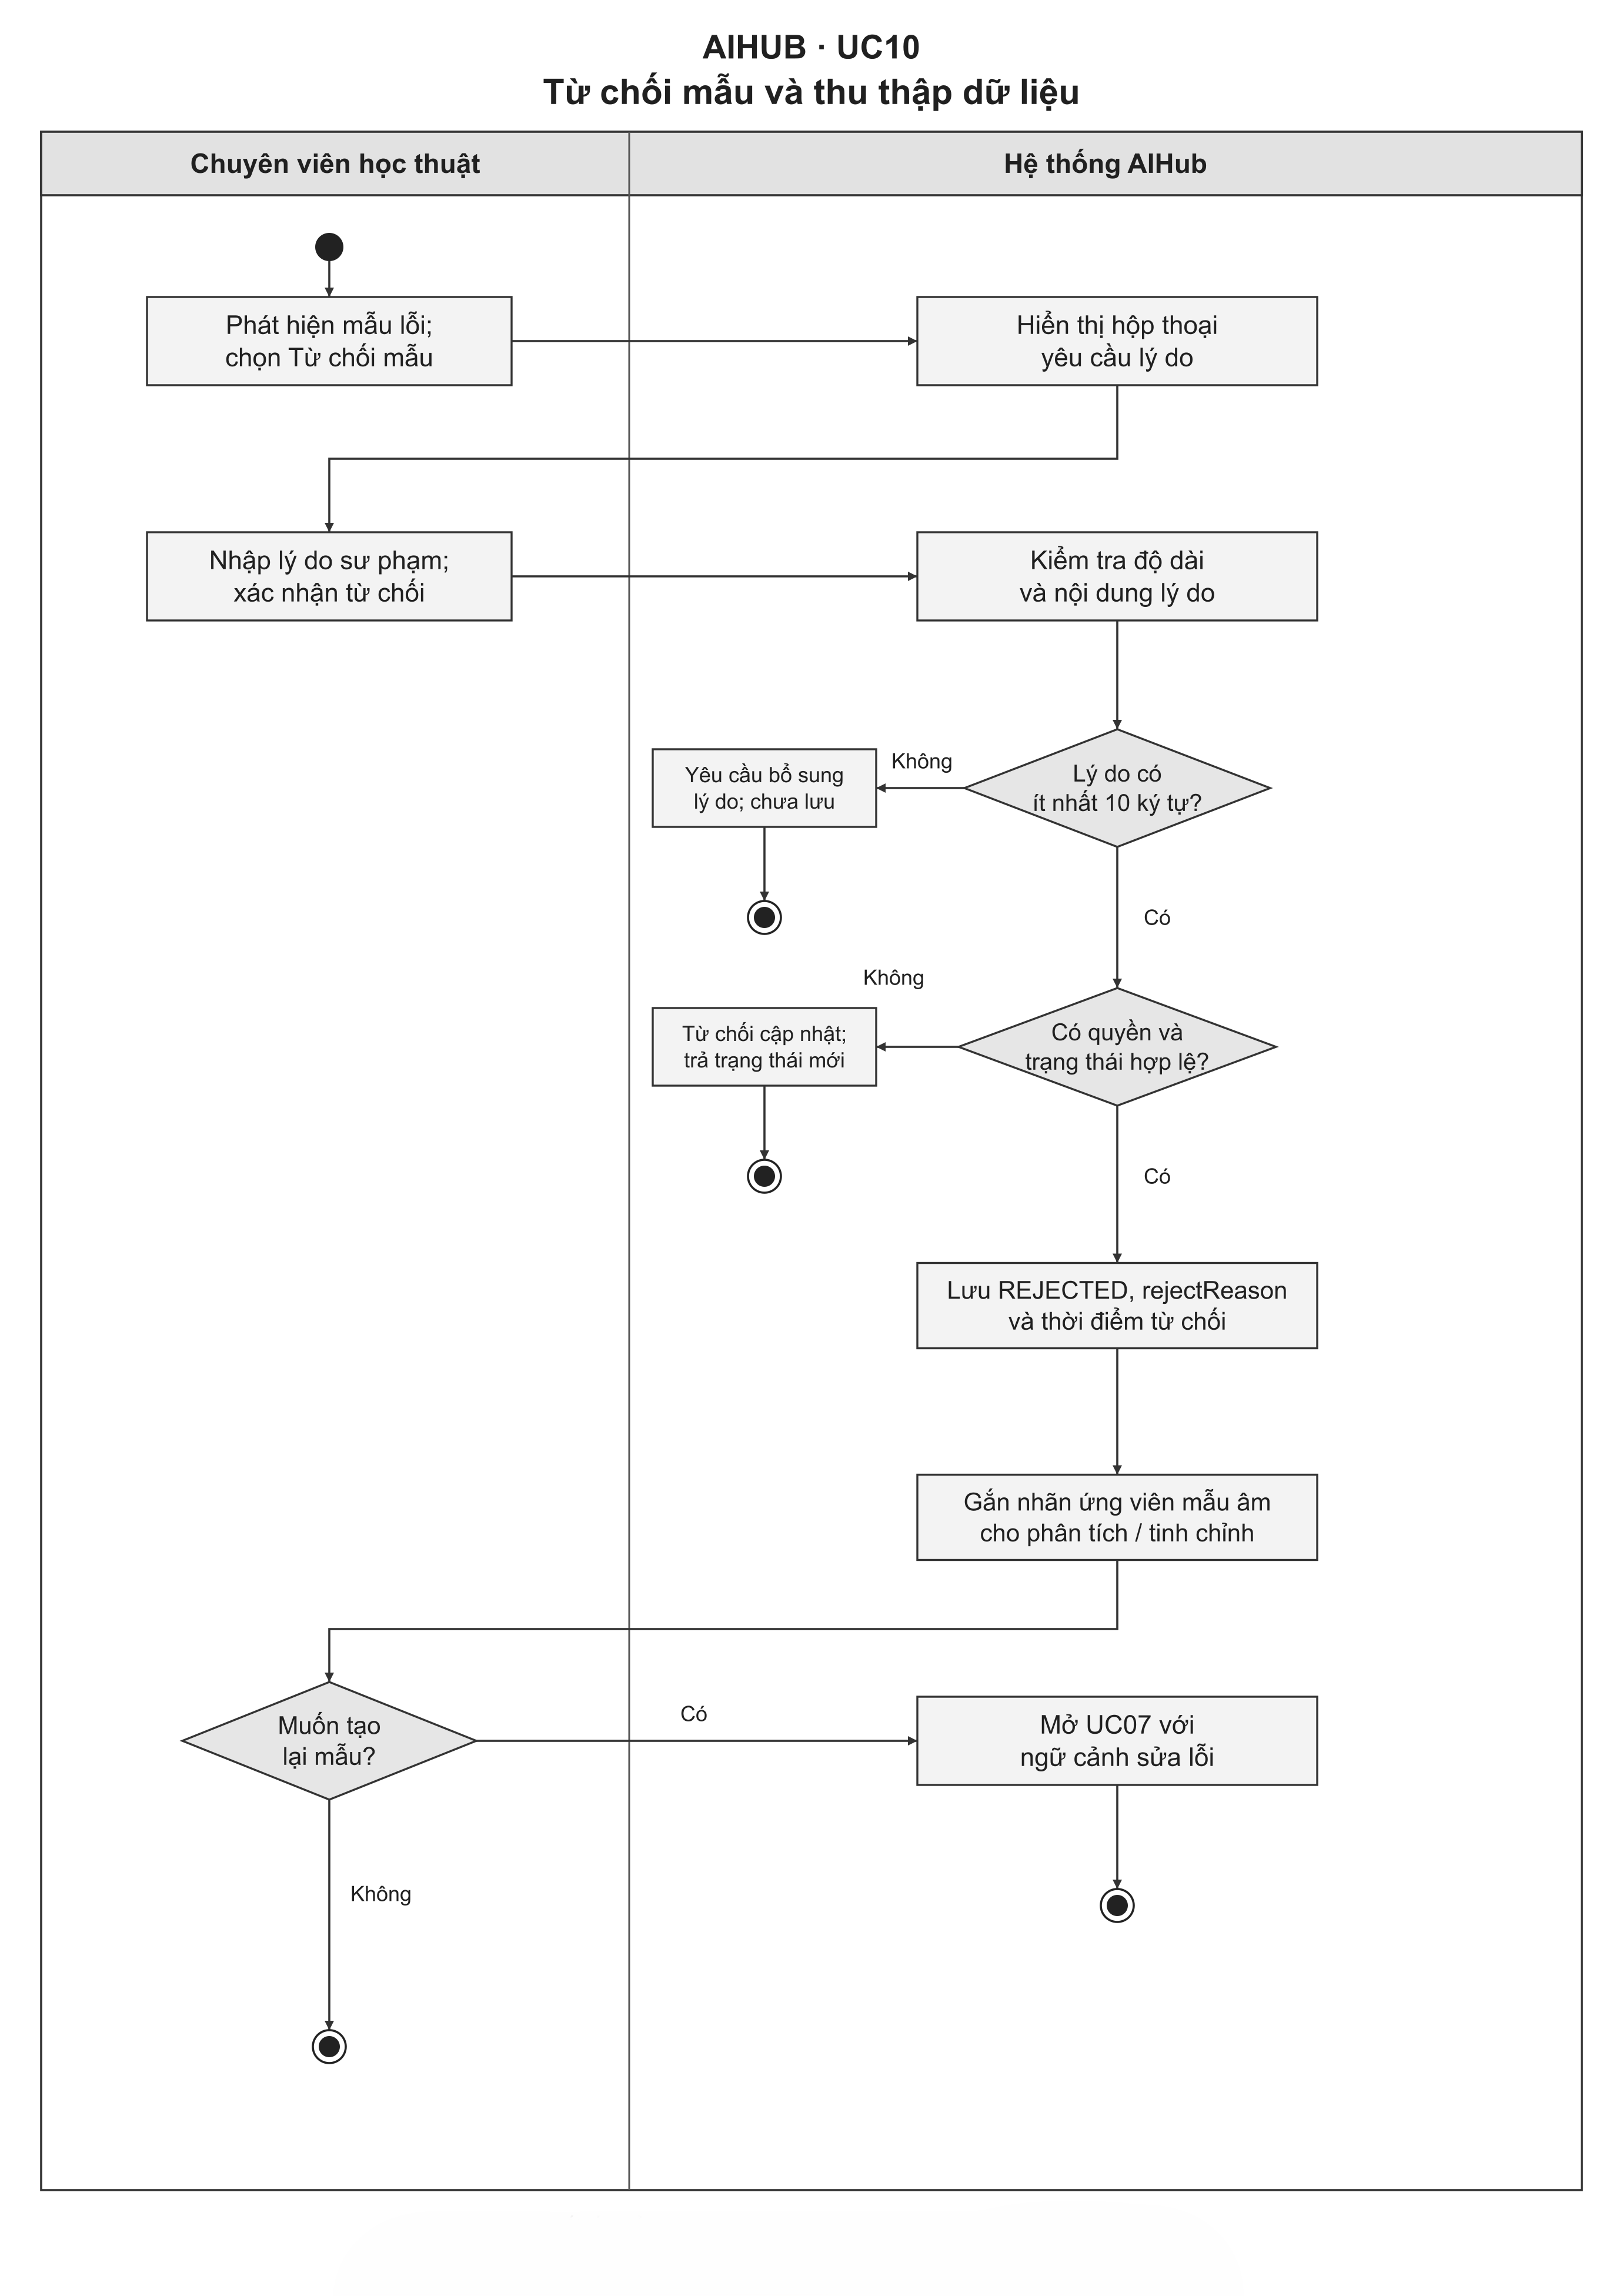
\includegraphics[width=\linewidth,height=0.72\textheight,keepaspectratio]{Images/Activity/AIHub/activity_uc10_reject_sample.png}
    \caption{Sơ đồ hoạt động AIHub -- Use-case 10: Từ chối mẫu và thu thập dữ liệu}
    \label{aihub:fig:activity_uc10}
    \label{aihub:fig:act_uc10_academic_reject}
\end{figure}

Chuyên viên chọn từ chối mẫu và nhập lý do. Dữ liệu được ghi nhận để phân tích lỗi và chuẩn bị dữ liệu tinh chỉnh.
% activity-generated:end


\clearpage

\paragraph{Luồng hoạt động: Quản lý kho dữ liệu mẫu học thuật (Use-case 11)}

% activity-generated:start
\begin{figure}[H]
    \centering
    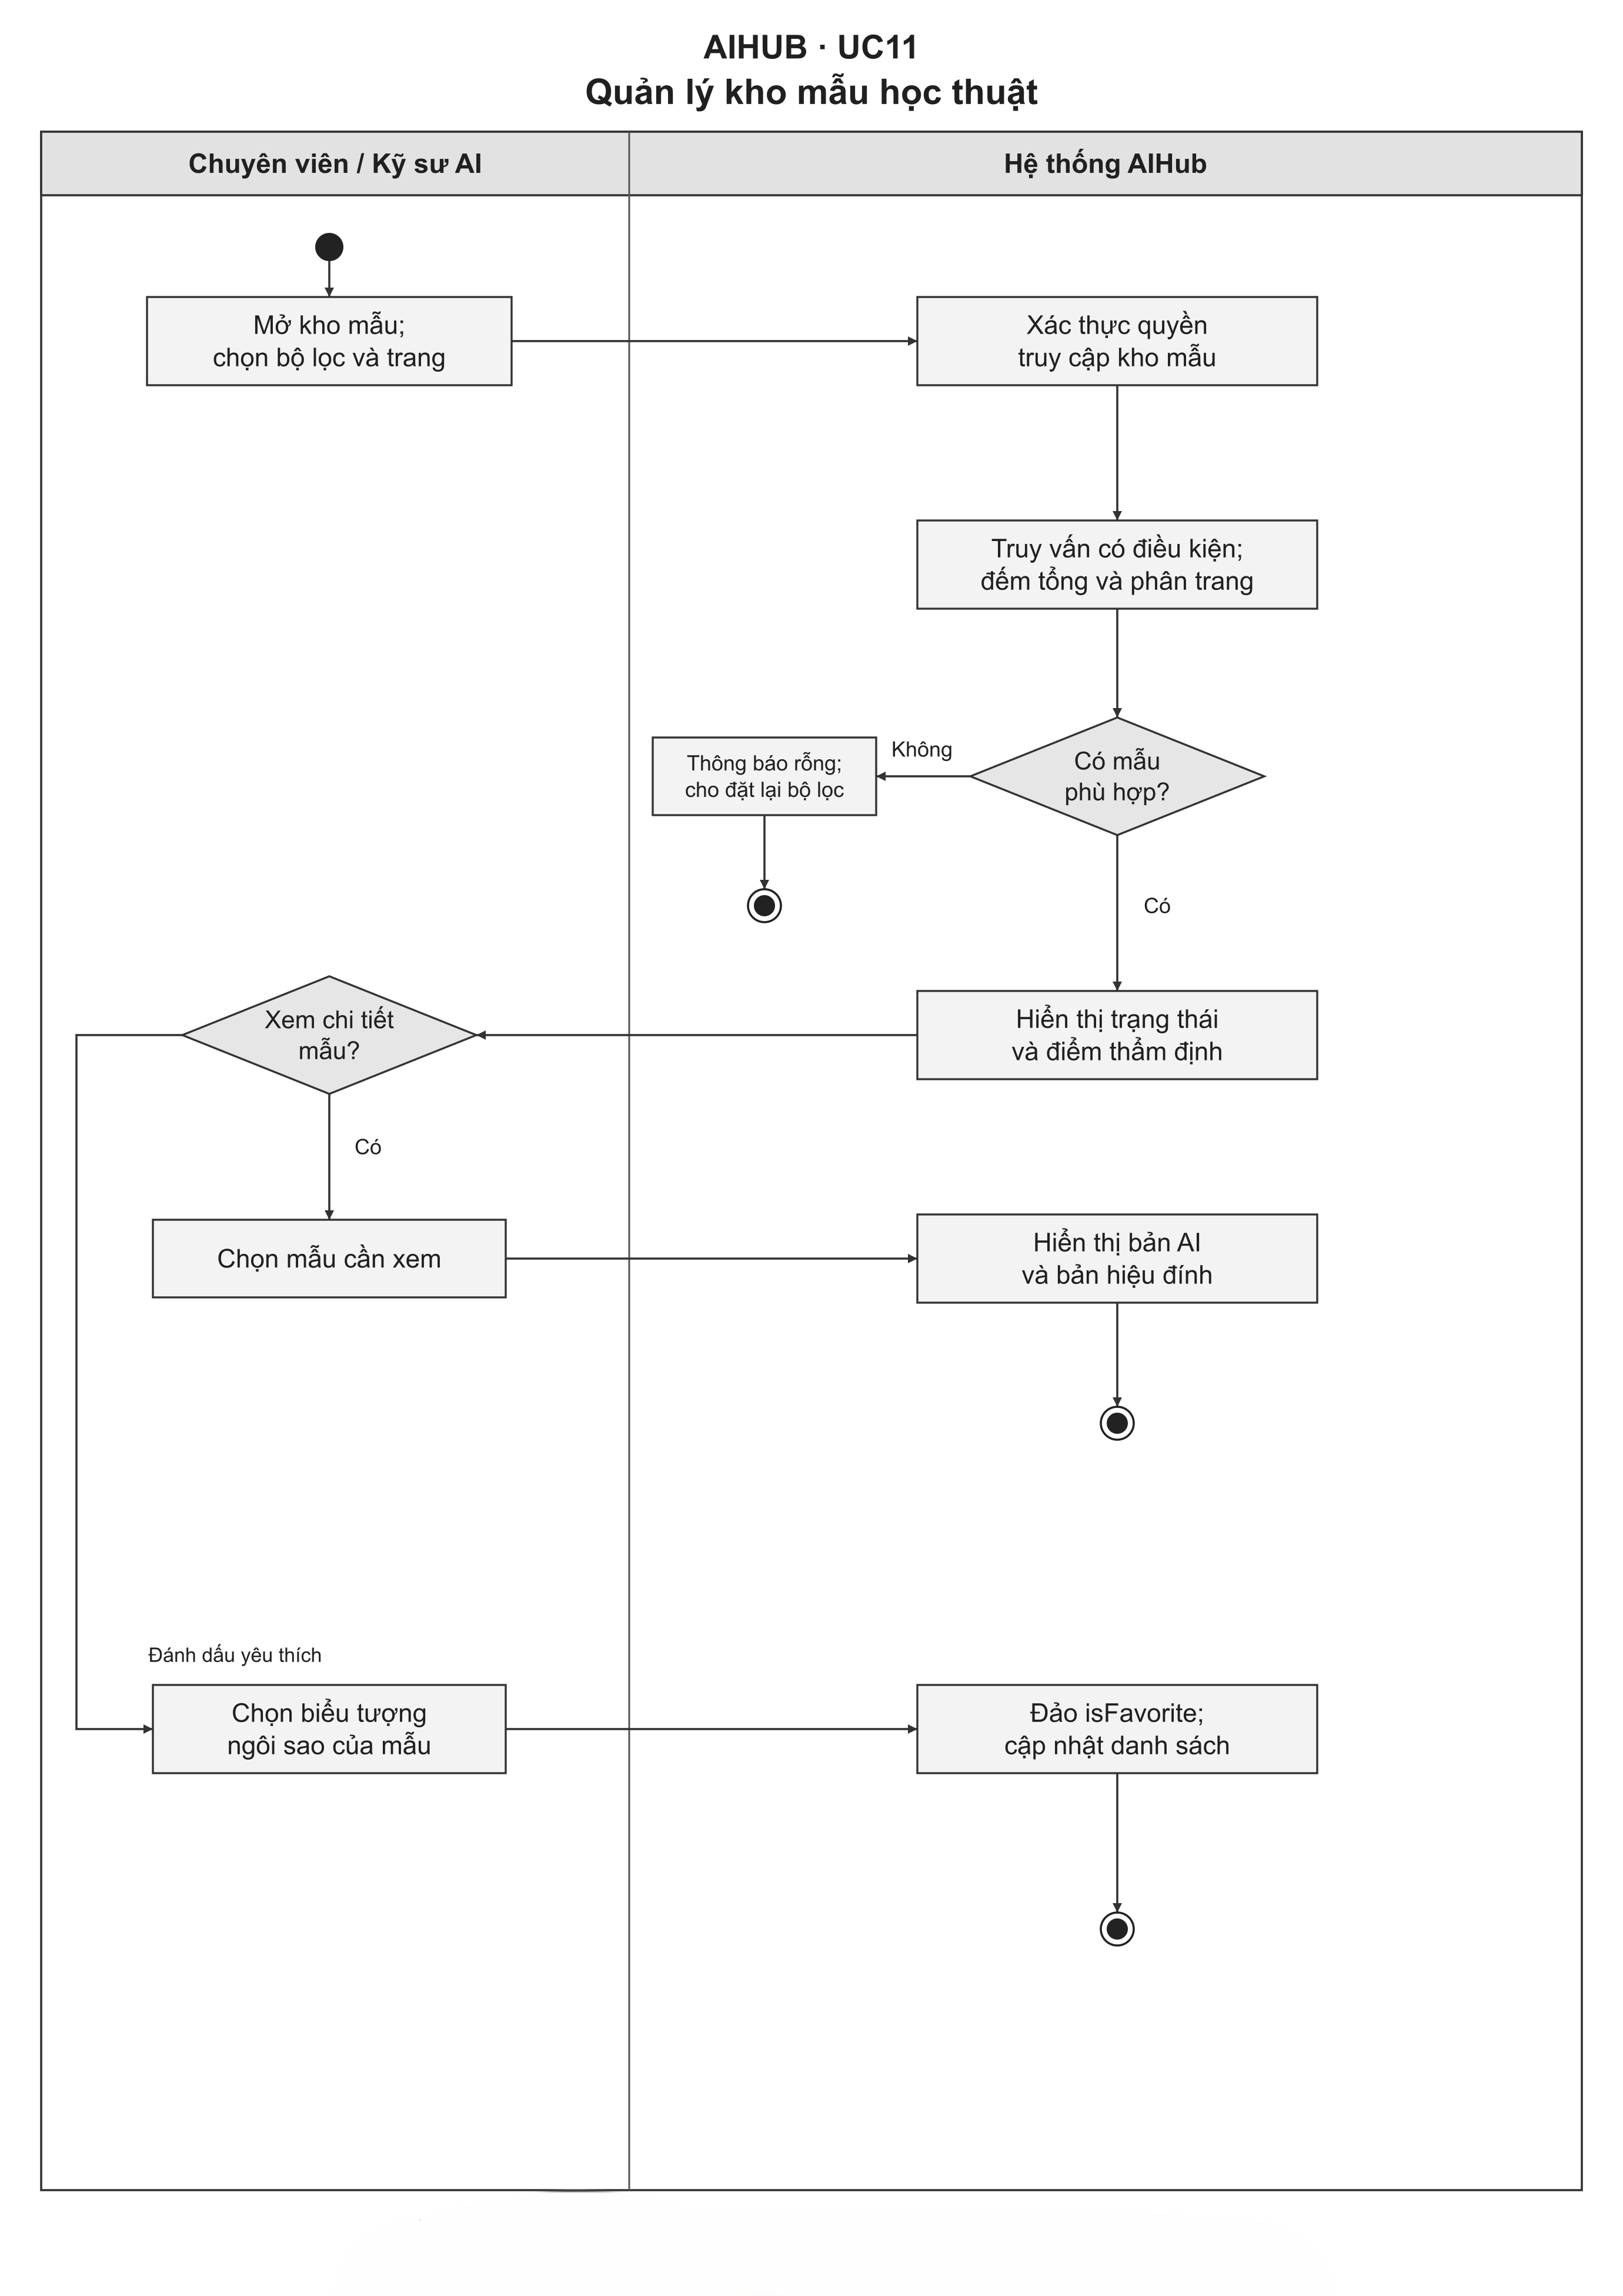
\includegraphics[width=\linewidth,height=0.72\textheight,keepaspectratio]{Images/Activity/AIHub/activity_uc11_academic_inventory.png}
    \caption{Sơ đồ hoạt động AIHub -- Use-case 11: Quản lý kho mẫu học thuật}
    \label{aihub:fig:activity_uc11}
    \label{aihub:fig:act_uc11_academic_inventory}
\end{figure}

Chuyên viên chọn bộ lọc để tra cứu kho mẫu. Thao tác đánh dấu yêu thích được lưu mà không thay đổi trạng thái thẩm định.
% activity-generated:end


% =========================================================================
% NHÓM 3: KỸ SƯ AI (USE-CASE 12 - 15)
% =========================================================================

\clearpage

\paragraph{Luồng hoạt động: Cấu hình mẫu Prompt (Use-case 12)}

% activity-generated:start
\begin{figure}[H]
    \centering
    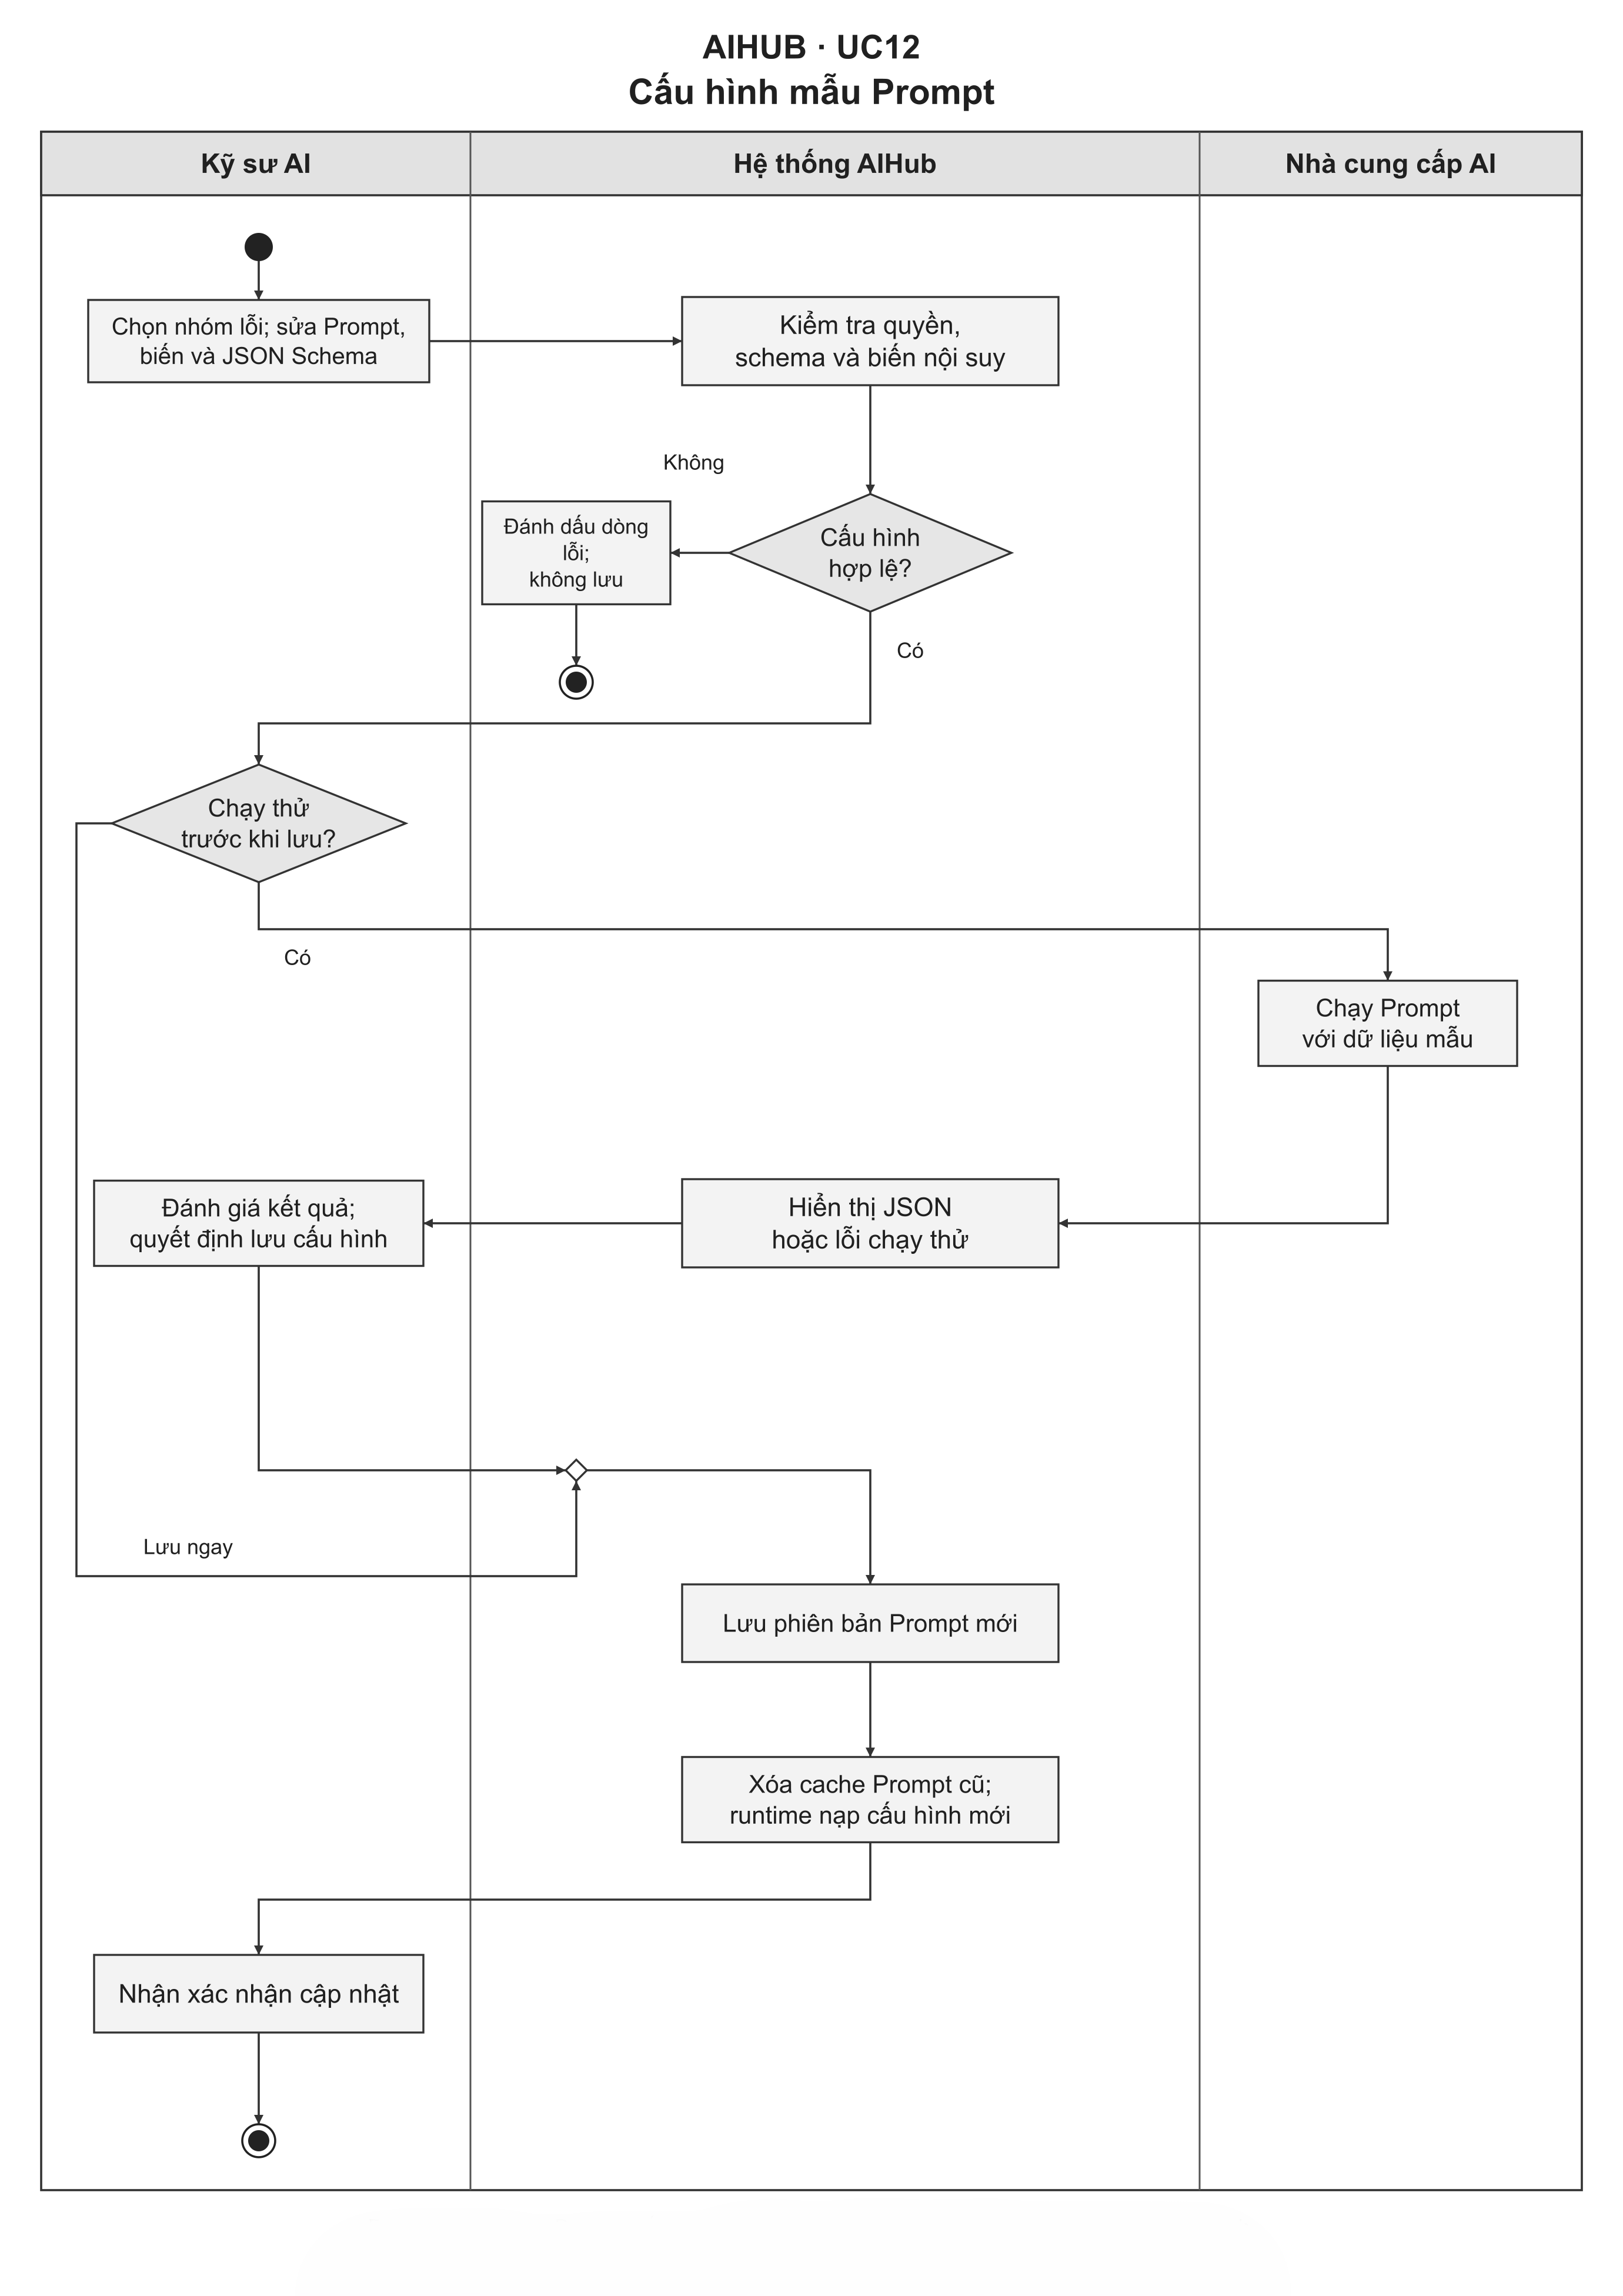
\includegraphics[width=\linewidth,height=0.72\textheight,keepaspectratio]{Images/Activity/AIHub/activity_uc12_prompt_templates.png}
    \caption{Sơ đồ hoạt động AIHub -- Use-case 12: Cấu hình mẫu Prompt}
    \label{aihub:fig:activity_uc12}
    \label{aihub:fig:act_uc12_config_prompt}
\end{figure}

Quản trị viên mở cấu hình và chỉnh sửa mẫu Prompt. Hệ thống lưu phiên bản mới và cập nhật cấu hình được sử dụng.
% activity-generated:end


\clearpage

\paragraph{Luồng hoạt động: Cấu hình chuỗi mô hình dự phòng (Use-case 13)}

% activity-generated:start
\begin{figure}[H]
    \centering
    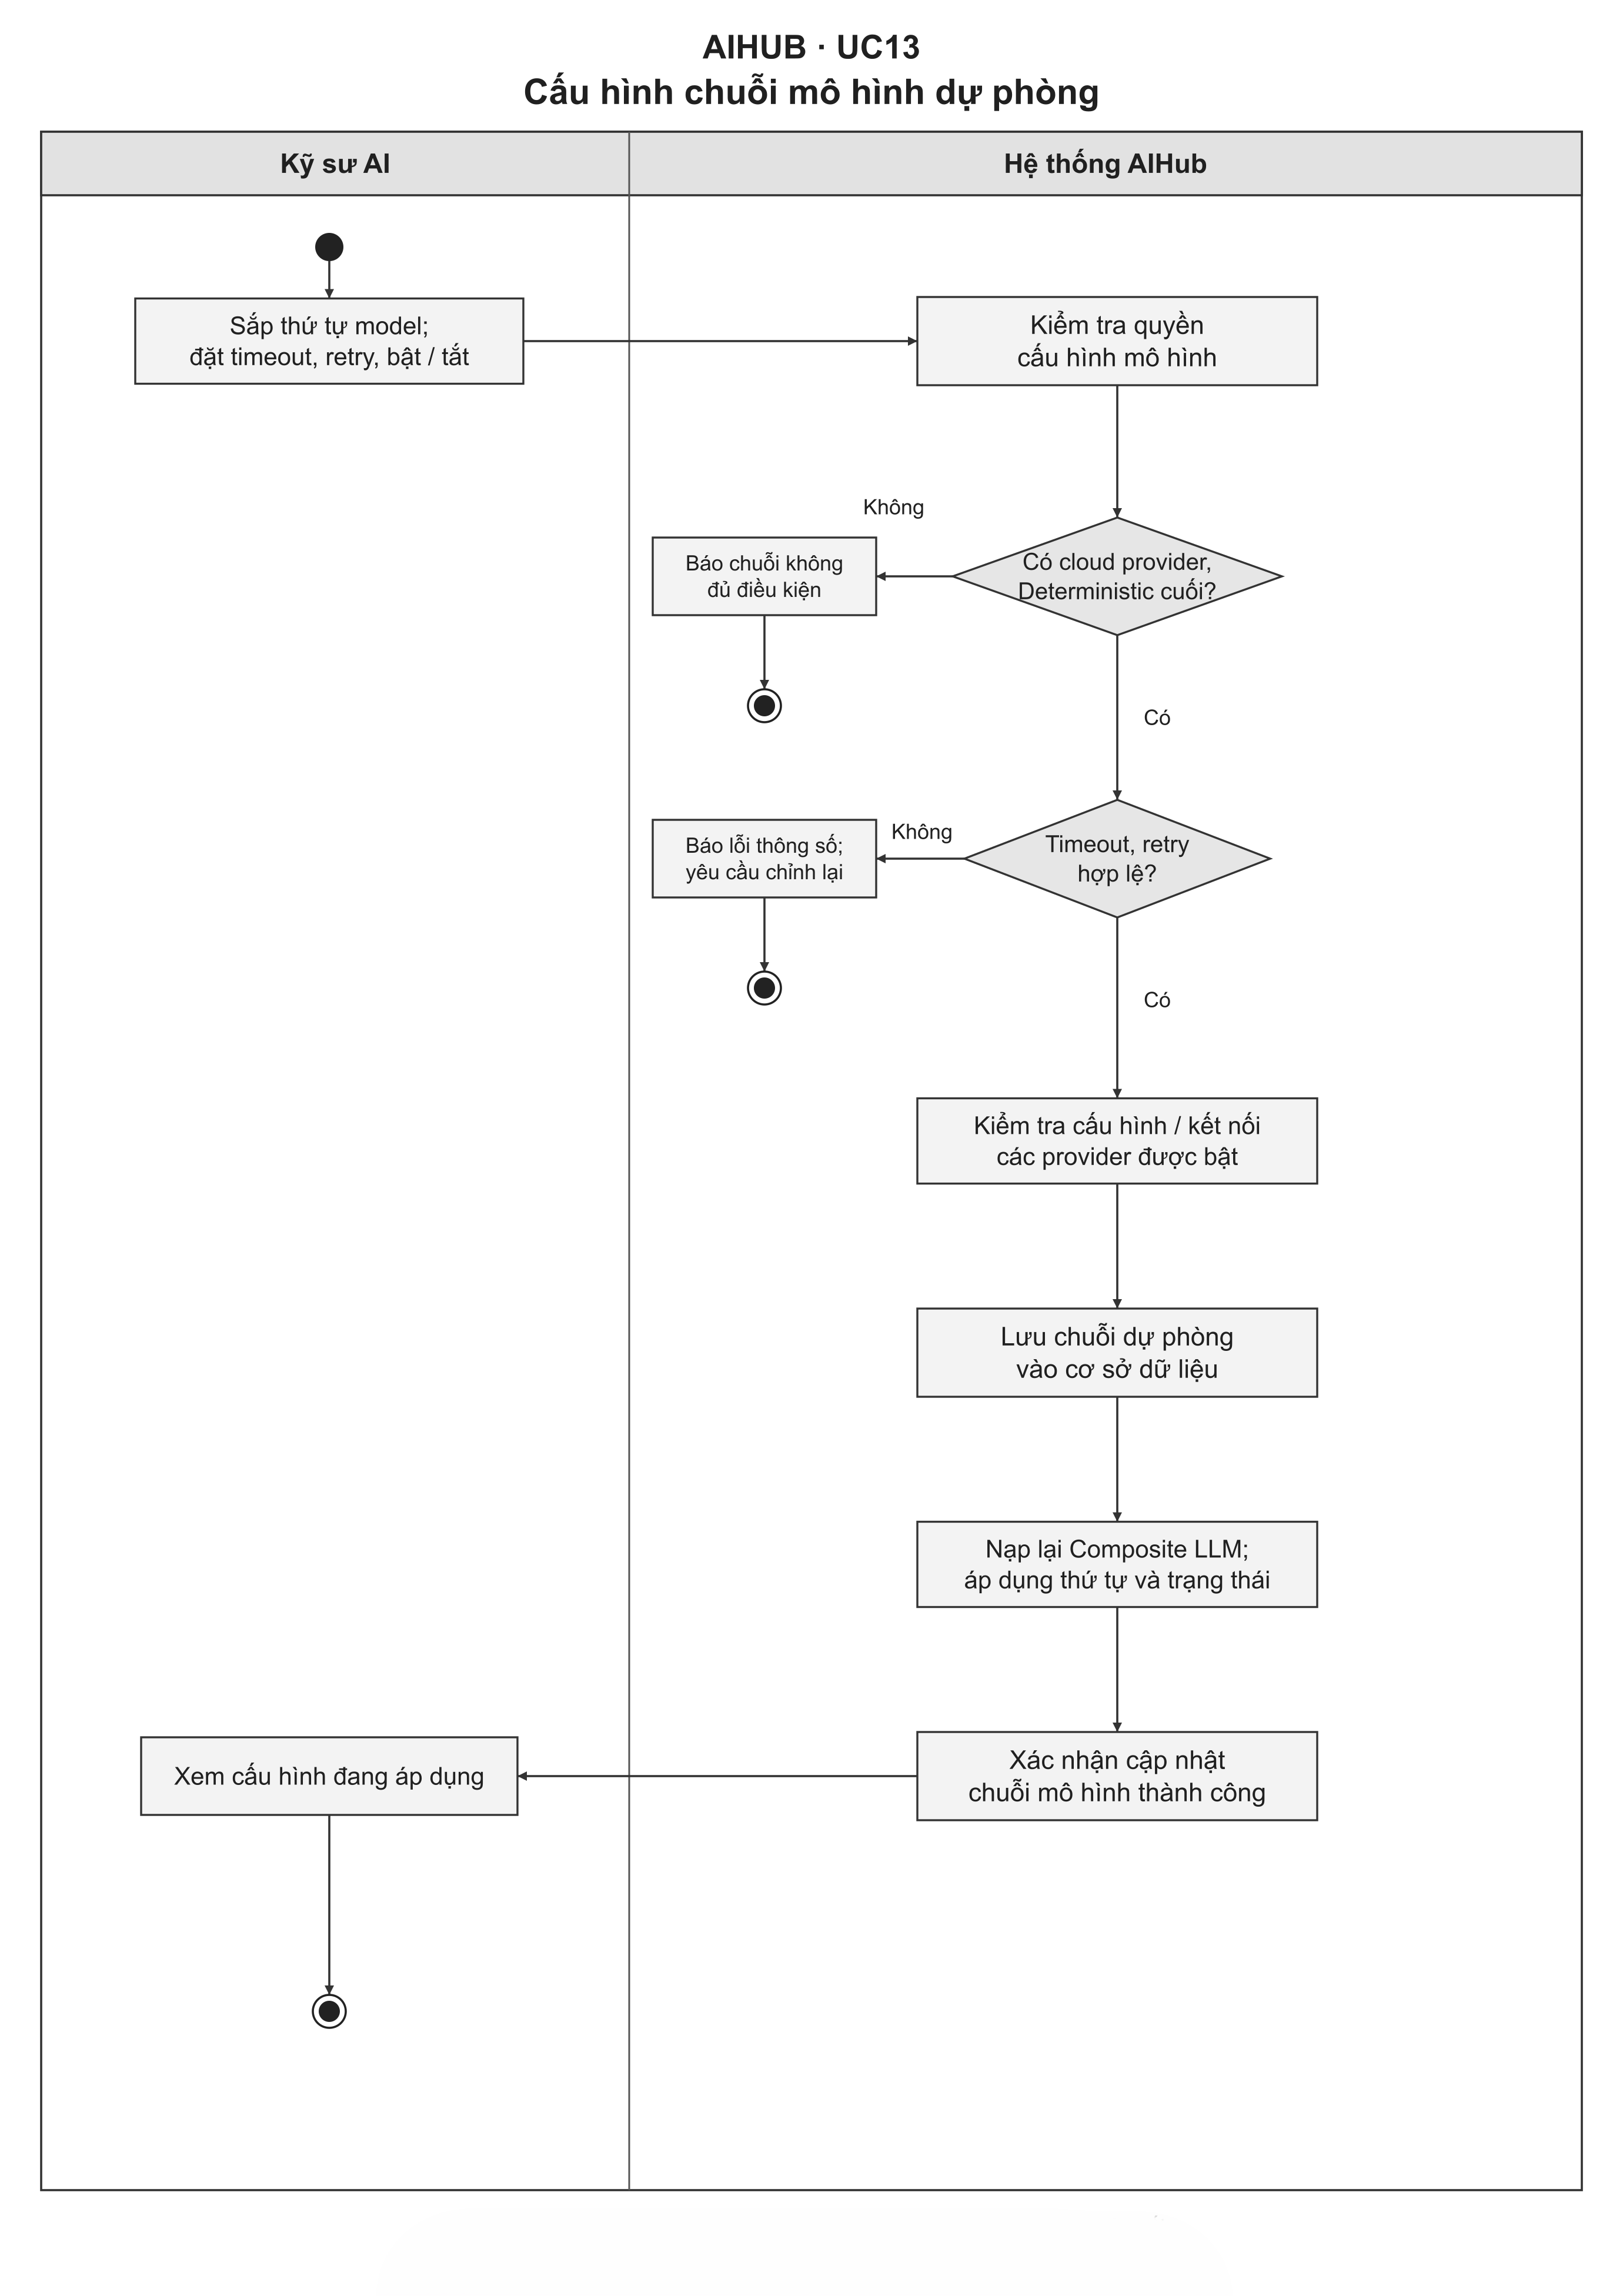
\includegraphics[width=\linewidth,height=0.72\textheight,keepaspectratio]{Images/Activity/AIHub/activity_uc13_model_fallback.png}
    \caption{Sơ đồ hoạt động AIHub -- Use-case 13: Cấu hình chuỗi mô hình dự phòng}
    \label{aihub:fig:activity_uc13}
    \label{aihub:fig:act_uc13_config_fallback}
\end{figure}

Quản trị viên chỉnh thứ tự, thời gian chờ và số lần thử của các mô hình. Hệ thống cập nhật chuỗi gọi mô hình và thông báo kết quả.
% activity-generated:end


\clearpage

\paragraph{Luồng hoạt động: Trích xuất tập dữ liệu tinh chỉnh SFT/DPO (Use-case 14)}

% activity-generated:start
\begin{figure}[H]
    \centering
    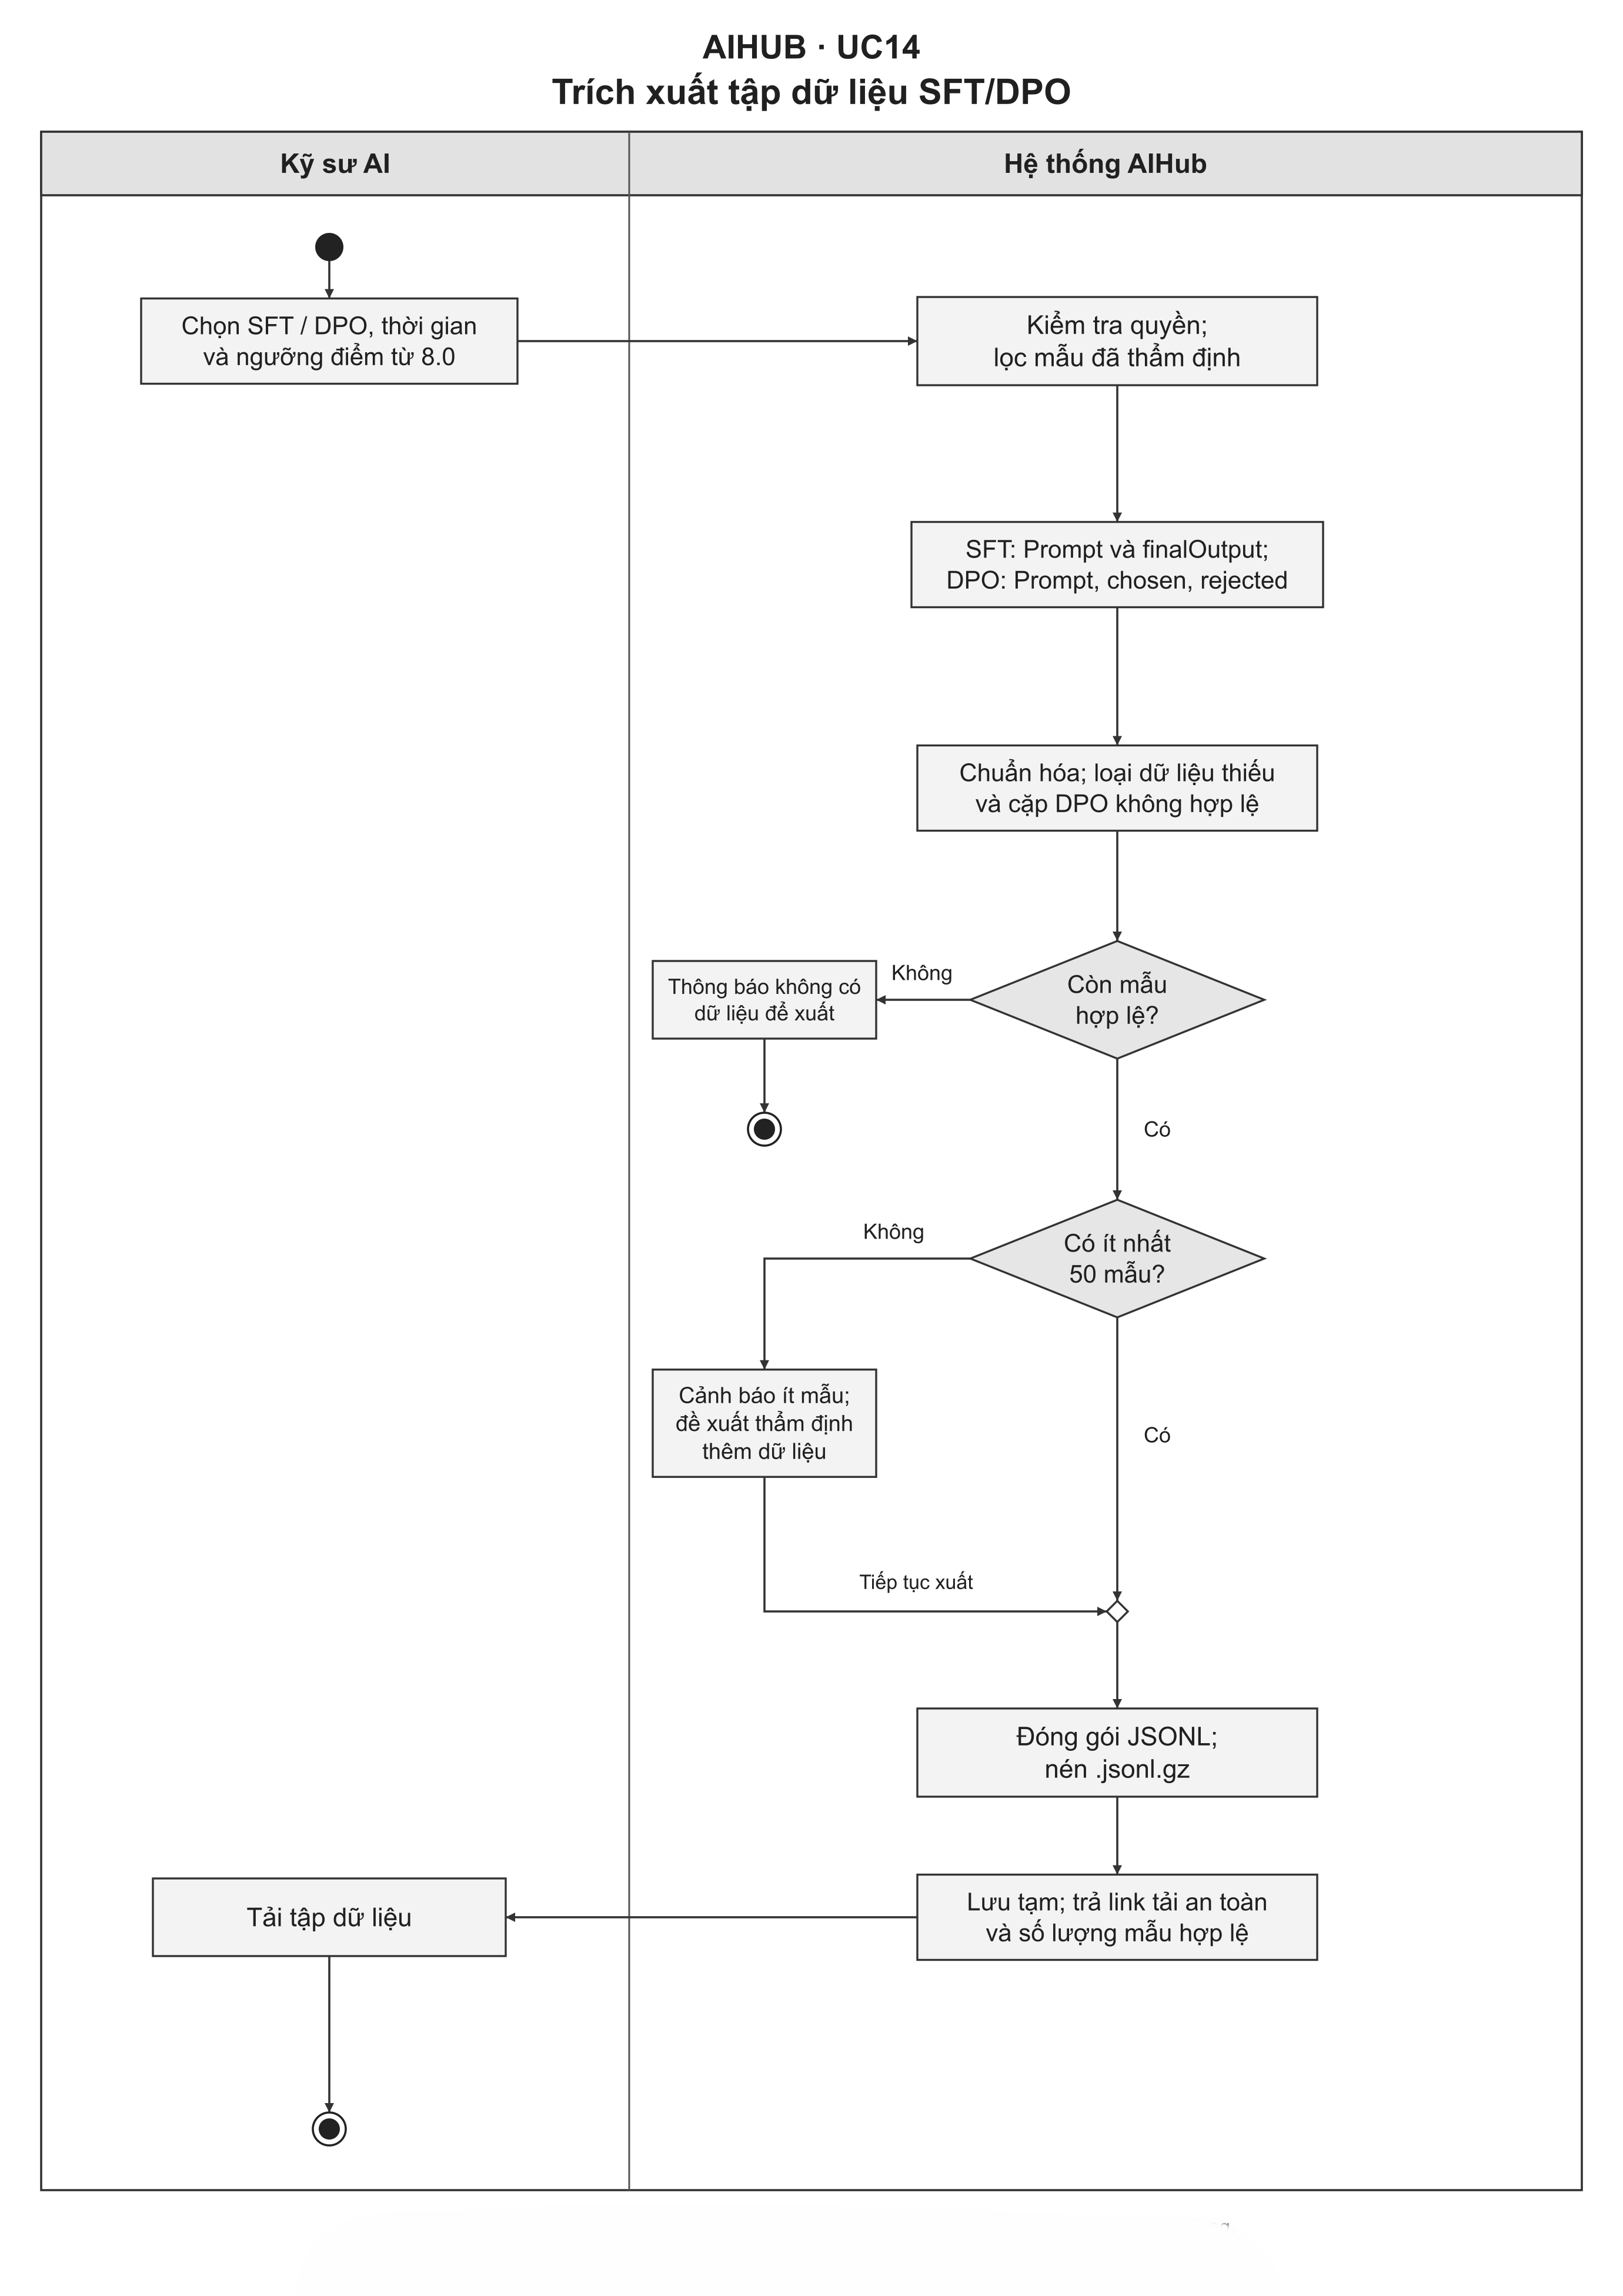
\includegraphics[width=\linewidth,height=0.72\textheight,keepaspectratio]{Images/Activity/AIHub/activity_uc14_export_datasets.png}
    \caption{Sơ đồ hoạt động AIHub -- Use-case 14: Trích xuất tập dữ liệu SFT/DPO}
    \label{aihub:fig:activity_uc14}
    \label{aihub:fig:act_uc14_export_datasets}
\end{figure}

Chuyên viên chọn loại dữ liệu SFT hoặc DPO và phạm vi xuất. Tập dữ liệu được tạo và cung cấp để tải xuống.
% activity-generated:end


\clearpage

\paragraph{Luồng hoạt động: Theo dõi và phân tích lỗi mô hình (Use-case 15)}

% activity-generated:start
\begin{figure}[H]
    \centering
    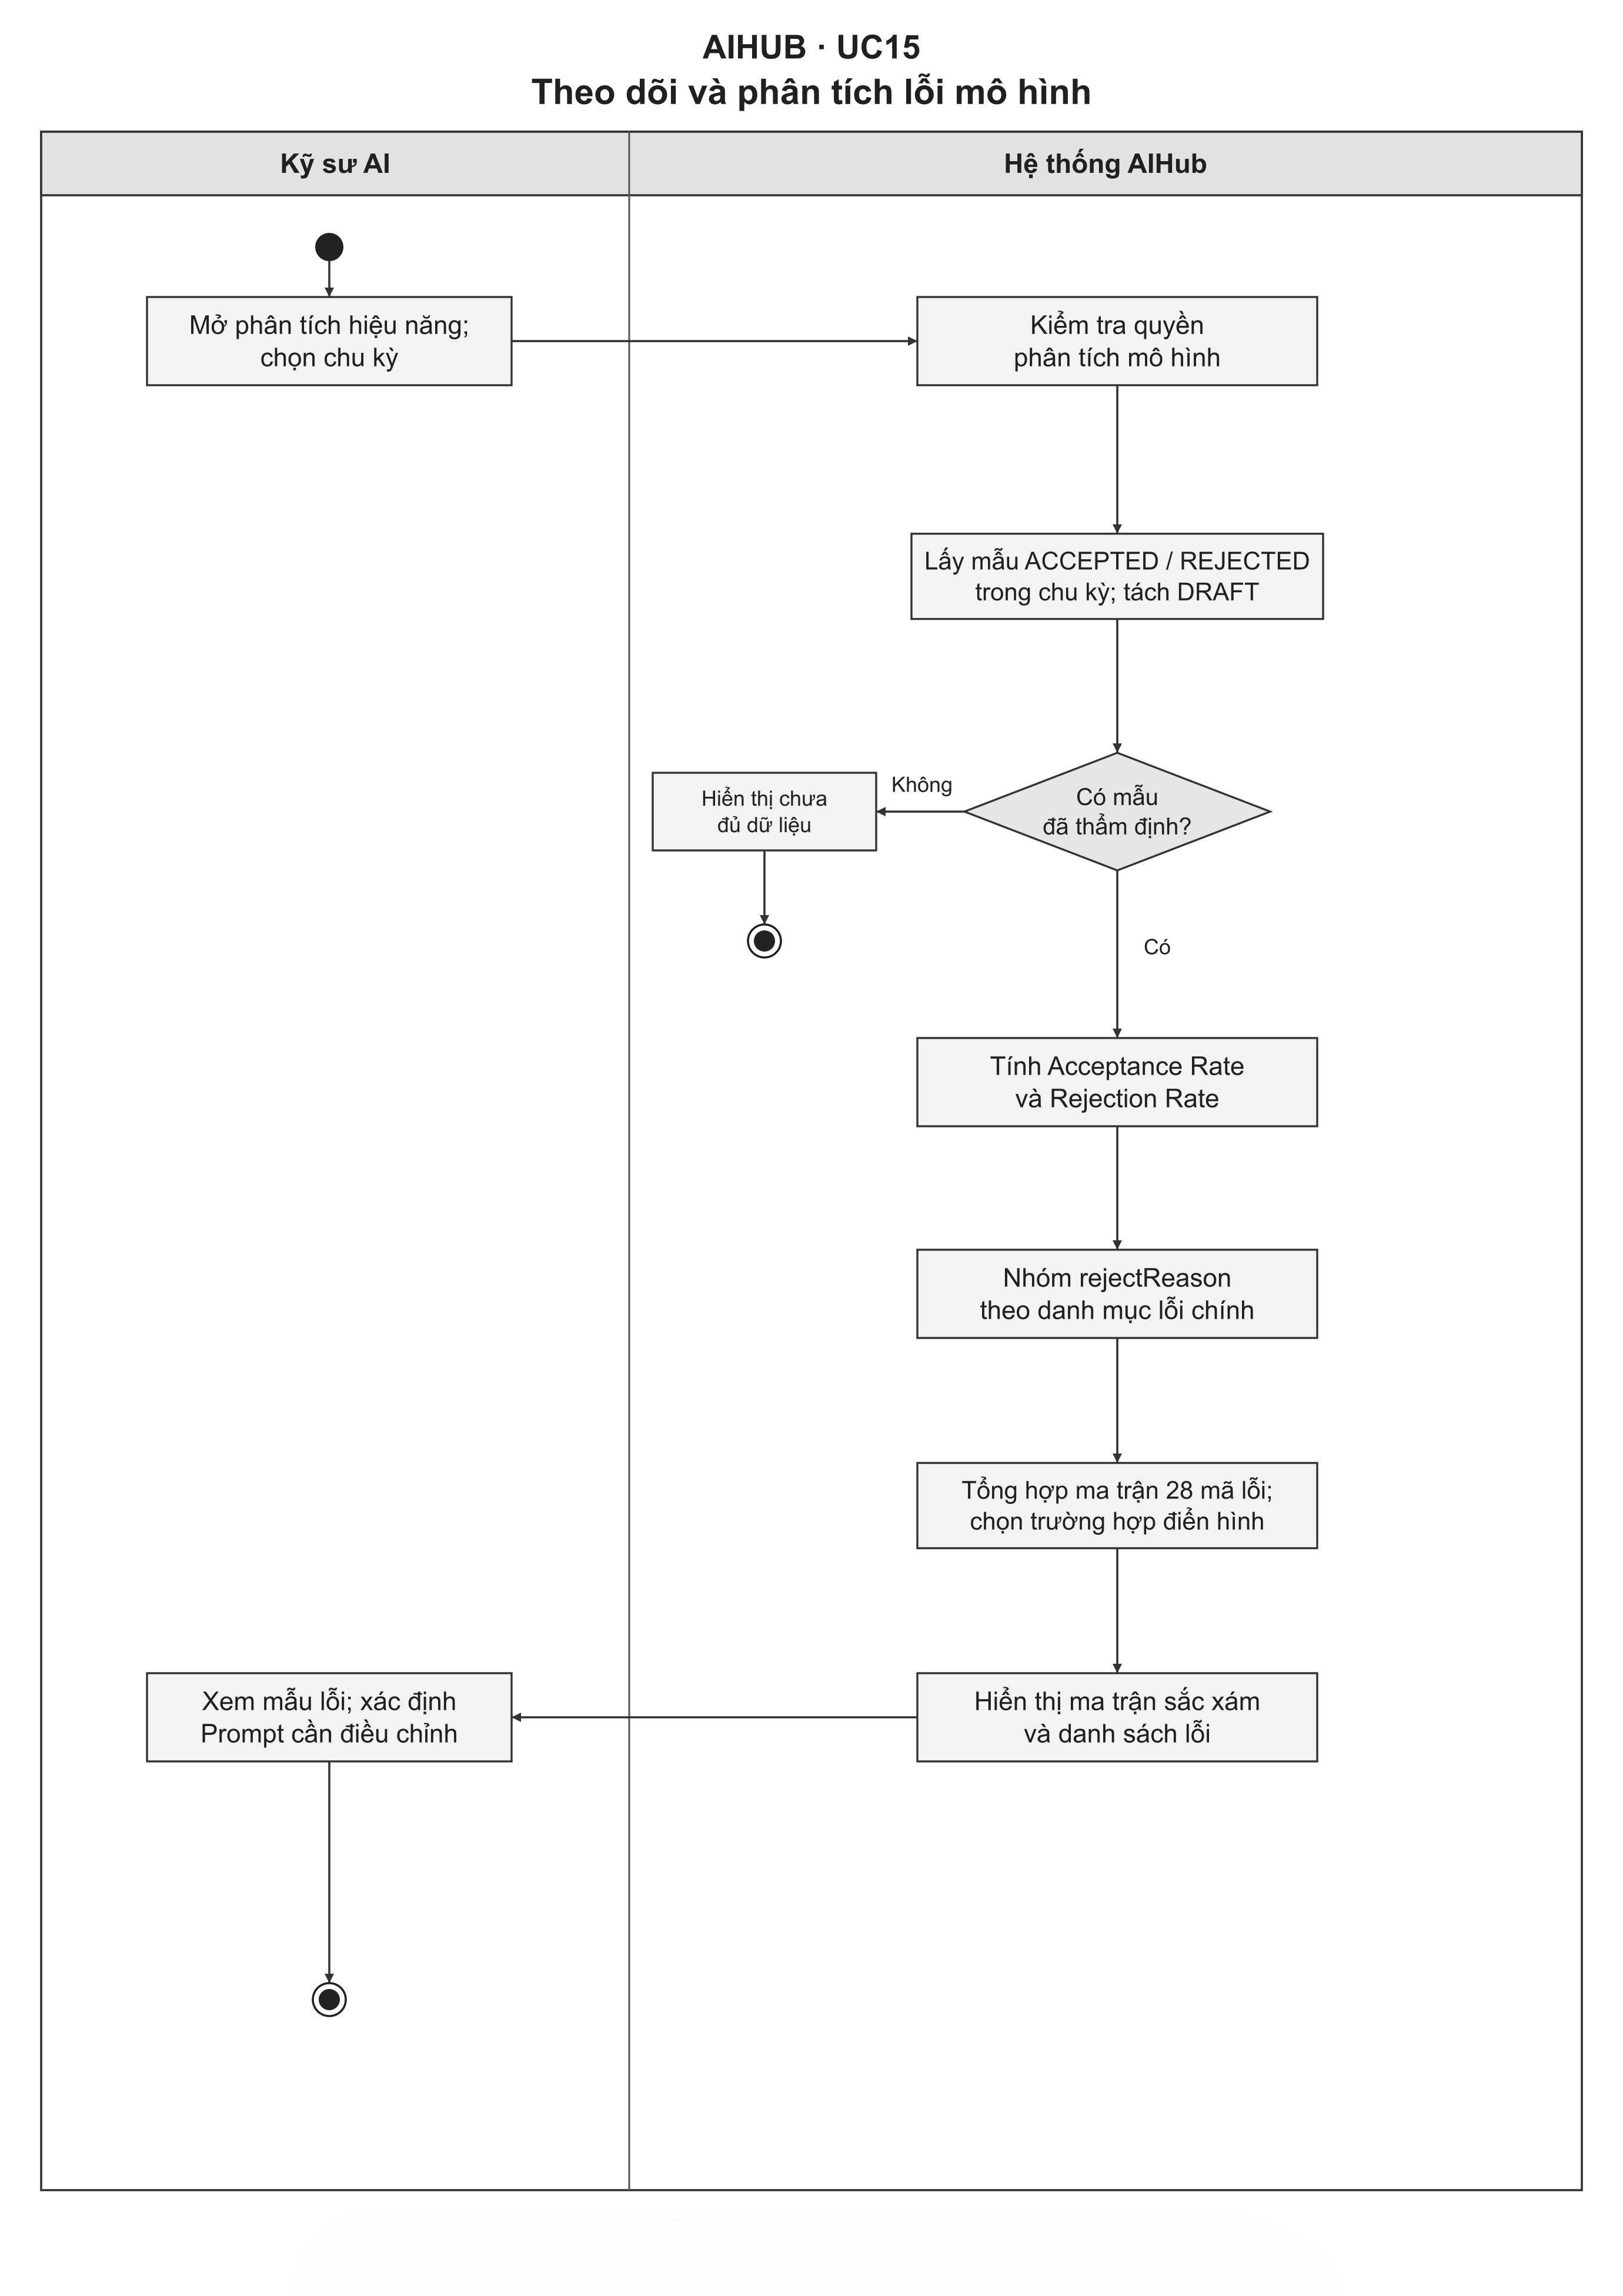
\includegraphics[width=\linewidth,height=0.72\textheight,keepaspectratio]{Images/Activity/AIHub/activity_uc15_model_error_analysis.png}
    \caption{Sơ đồ hoạt động AIHub -- Use-case 15: Theo dõi và phân tích lỗi mô hình}
    \label{aihub:fig:activity_uc15}
    \label{aihub:fig:act_uc15_analyze_model_errors}
\end{figure}

Người dùng chọn bộ lọc thống kê chất lượng mô hình. Người dùng xem chi tiết nhóm lỗi để xác định nội dung cần cải thiện.
% activity-generated:end


% =========================================================================
% NHÓM 4: QUẢN TRỊ VIÊN TỔ CHỨC & NỀN TẢNG (USE-CASE 16 - 20)
% =========================================================================

\clearpage

\paragraph{Luồng hoạt động: Quản lý thành viên tổ chức (Use-case 16)}

% activity-generated:start
\begin{figure}[H]
    \centering
    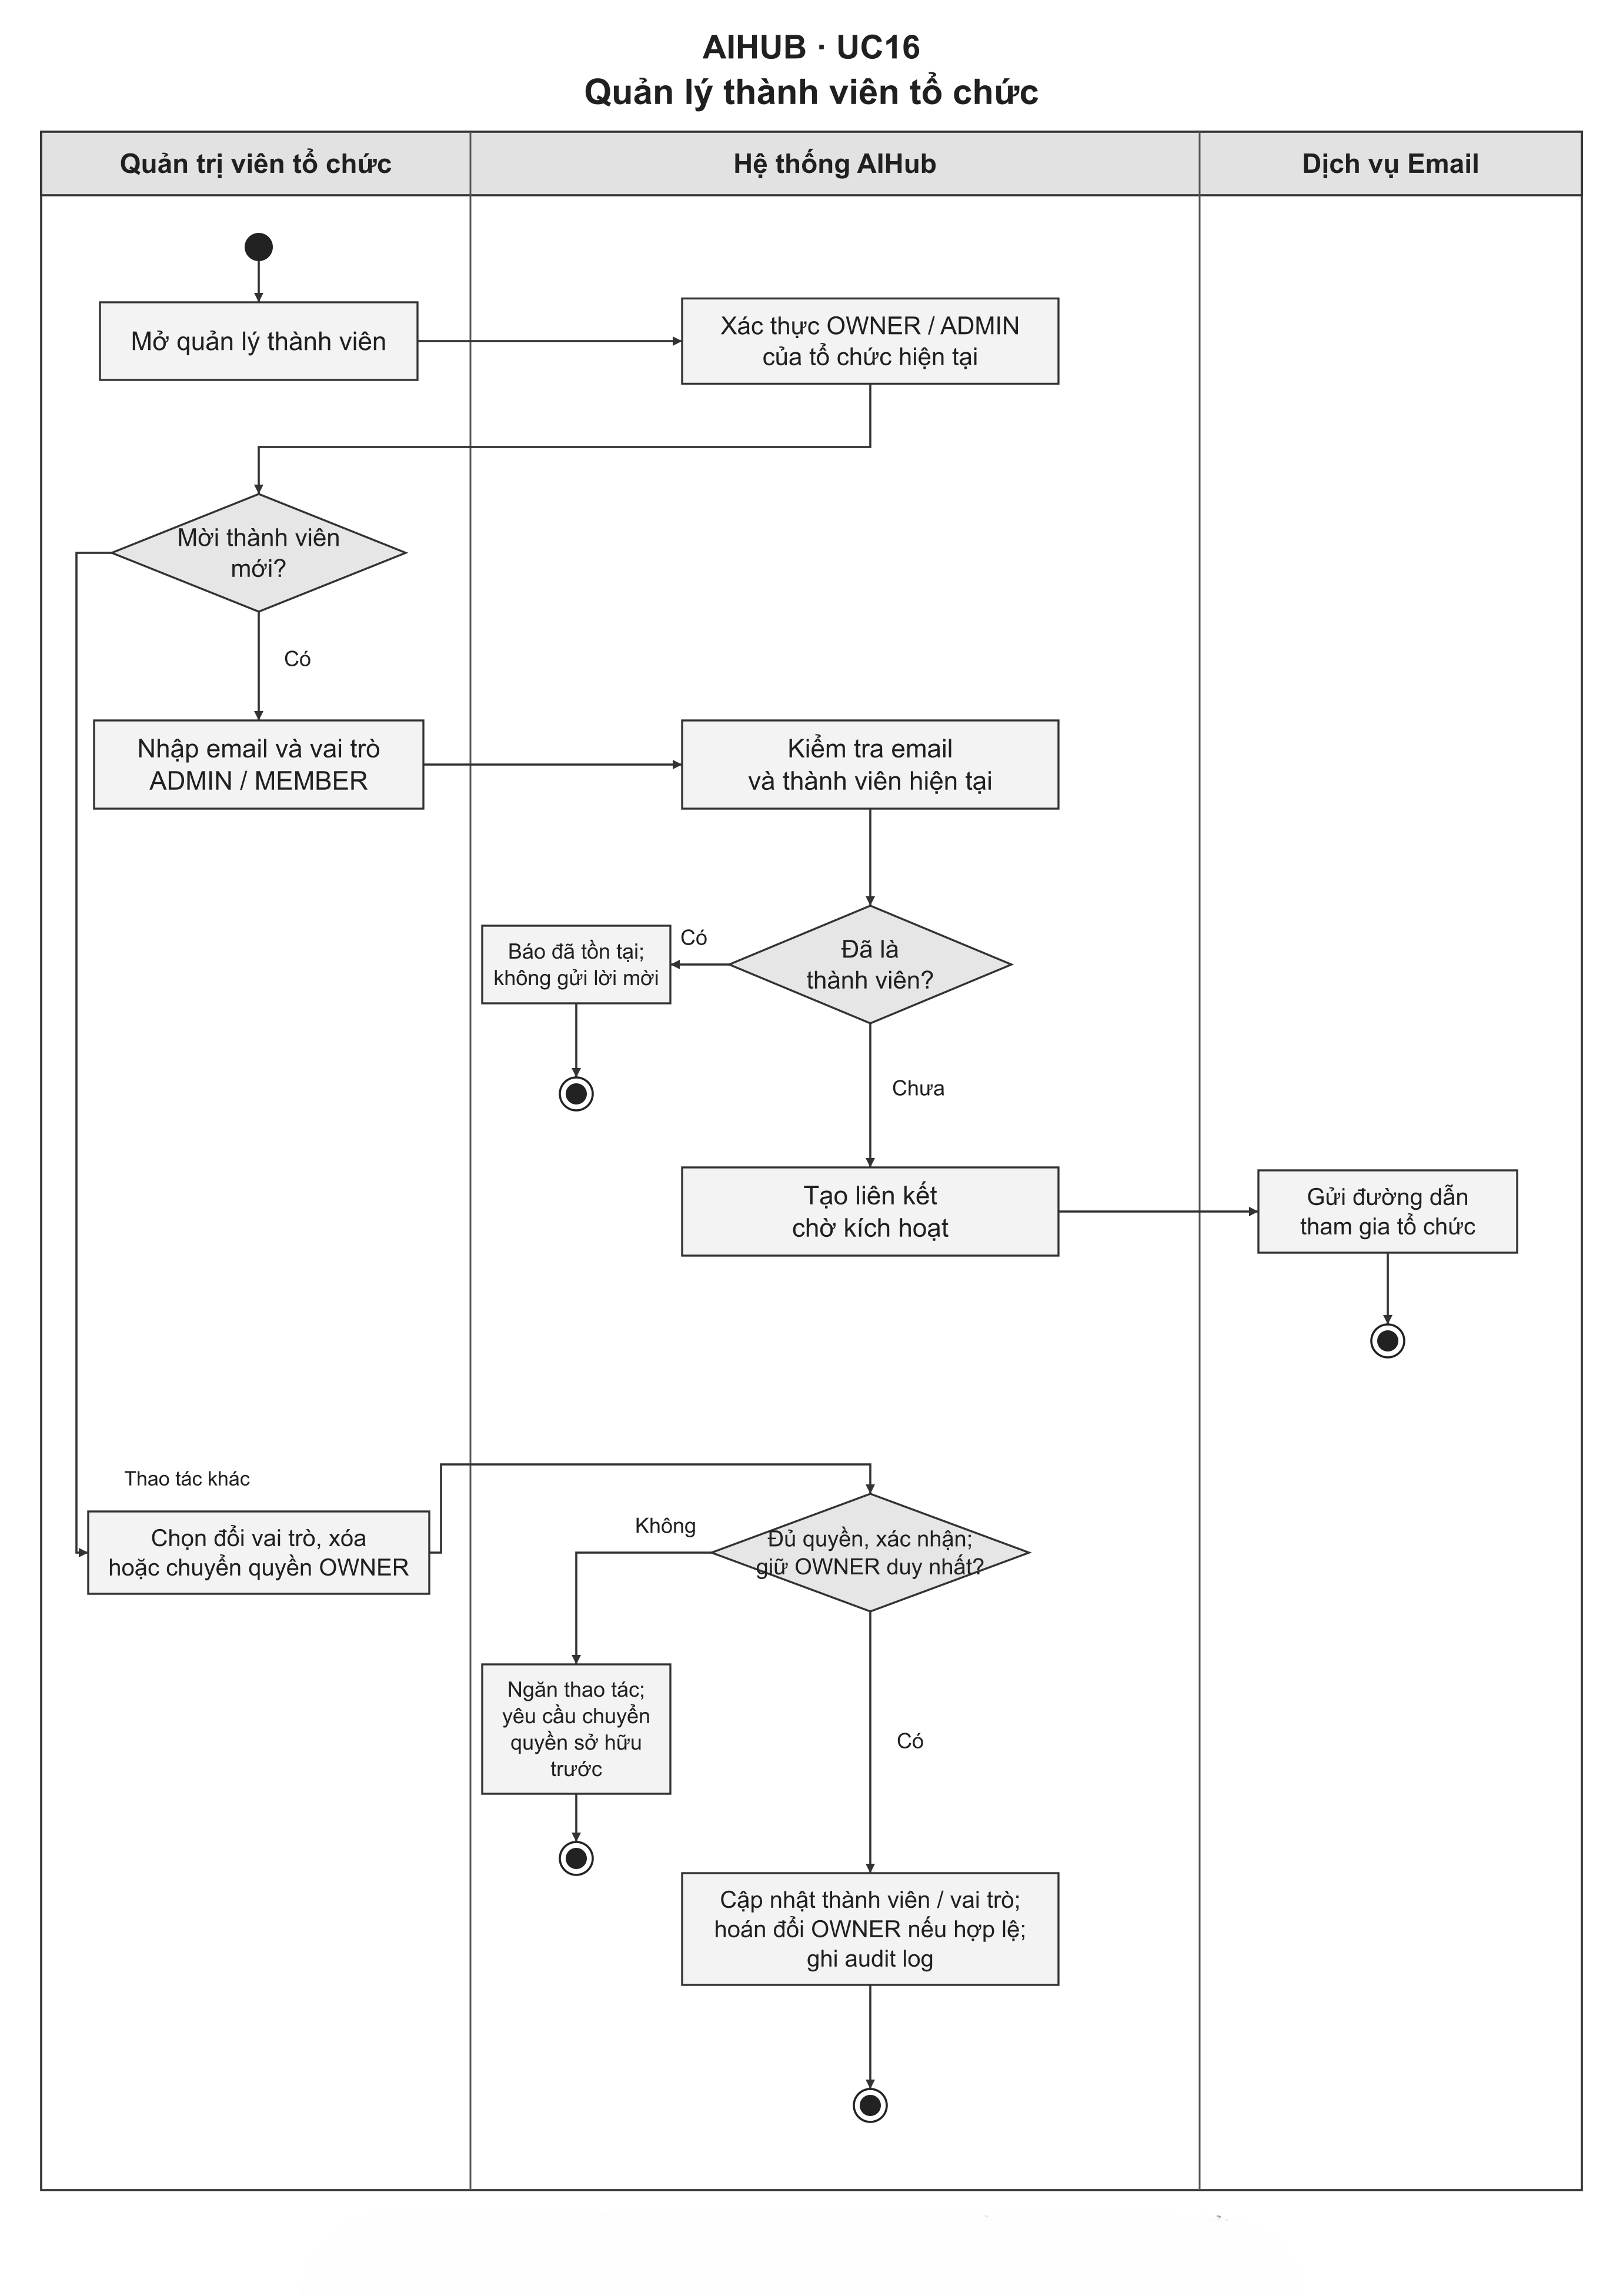
\includegraphics[width=\linewidth,height=0.72\textheight,keepaspectratio]{Images/Activity/AIHub/activity_uc16_organization_members.png}
    \caption{Sơ đồ hoạt động AIHub -- Use-case 16: Quản lý thành viên tổ chức}
    \label{aihub:fig:activity_uc16}
    \label{aihub:fig:act_uc16_manage_org_members}
\end{figure}

Người quản trị tổ chức chọn mời, đổi vai trò, xóa thành viên hoặc chuyển quyền. Hệ thống gửi thông báo và ghi nhật ký thay đổi.
% activity-generated:end


\clearpage

\paragraph{Luồng hoạt động: Quản trị gói cước và Hạn mức (Use-case 17)}

% activity-generated:start
\begin{figure}[H]
    \centering
    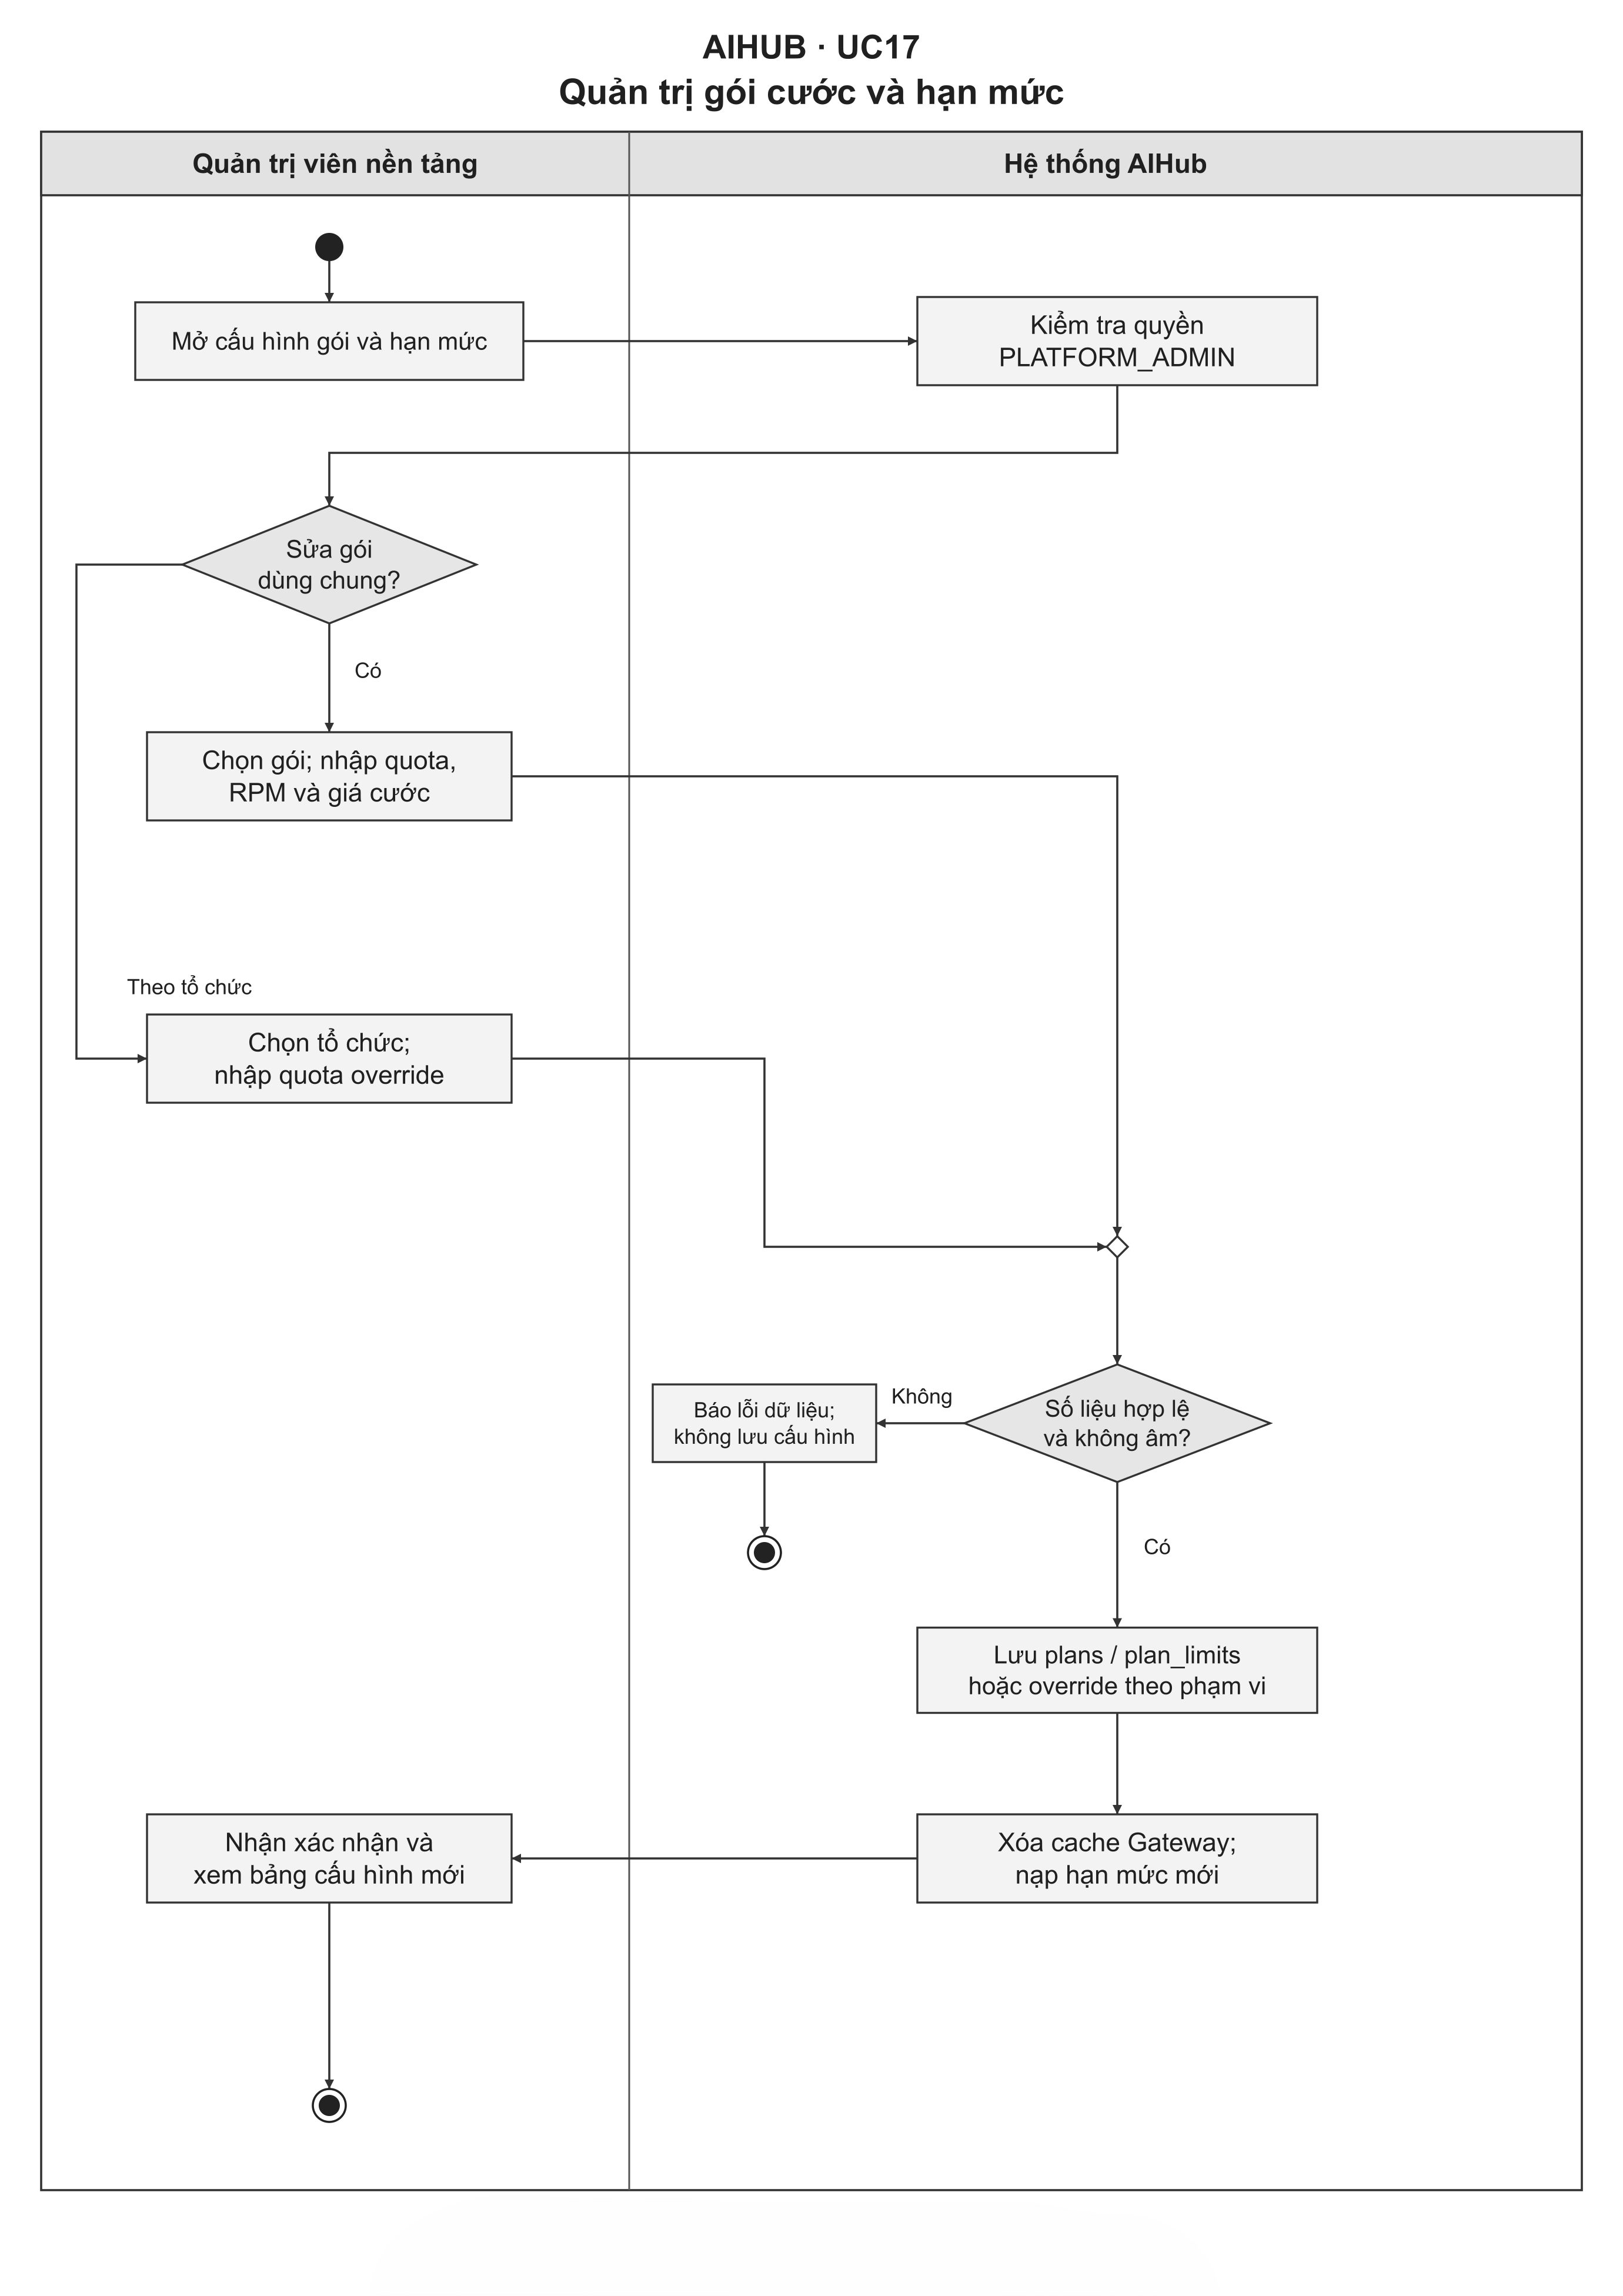
\includegraphics[width=\linewidth,height=0.72\textheight,keepaspectratio]{Images/Activity/AIHub/activity_uc17_plans_quota.png}
    \caption{Sơ đồ hoạt động AIHub -- Use-case 17: Quản trị gói cước và hạn mức}
    \label{aihub:fig:activity_uc17}
    \label{aihub:fig:act_uc17_config_plans}
\end{figure}

Quản trị viên chọn chỉnh gói dùng chung hoặc hạn mức riêng của tổ chức. Gateway cập nhật hạn mức và giao diện hiển thị kết quả.
% activity-generated:end


\clearpage

\paragraph{Luồng hoạt động: Giám sát trạng thái toàn hệ thống (Use-case 18)}

% activity-generated:start
\begin{figure}[H]
    \centering
    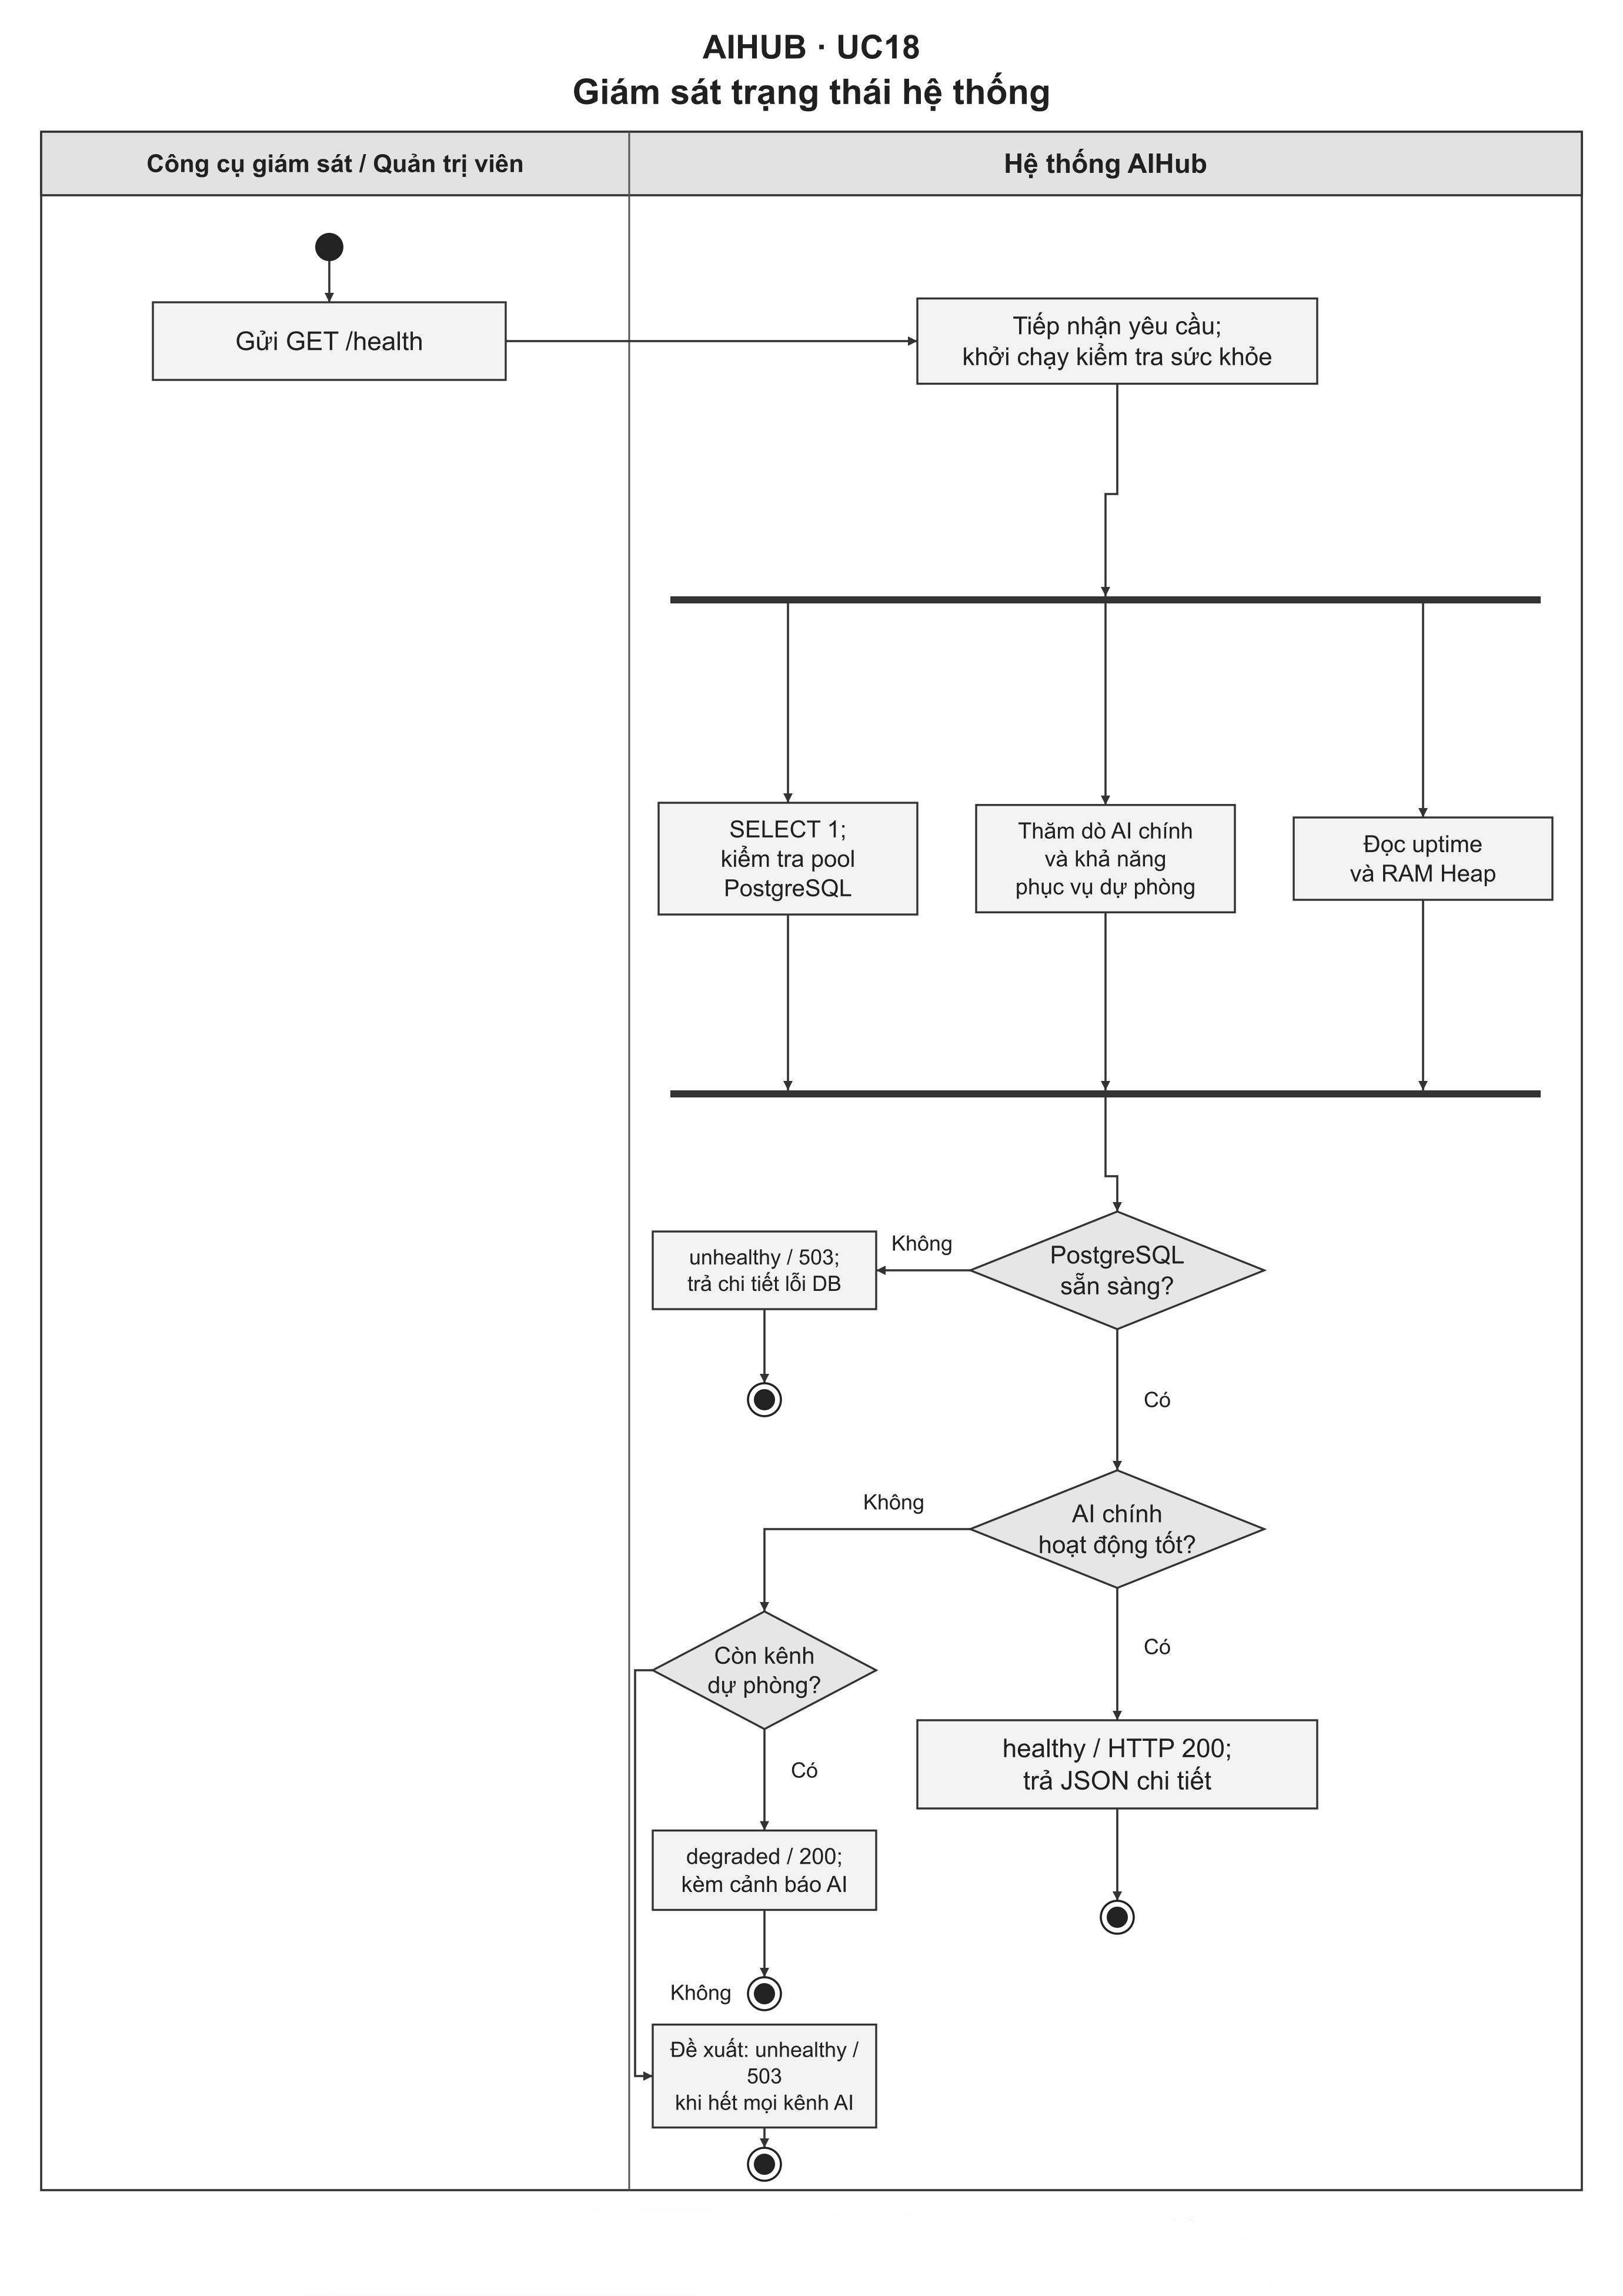
\includegraphics[width=\linewidth,height=0.72\textheight,keepaspectratio]{Images/Activity/AIHub/activity_uc18_system_health.png}
    \caption{Sơ đồ hoạt động AIHub -- Use-case 18: Giám sát trạng thái hệ thống}
    \label{aihub:fig:activity_uc18}
    \label{aihub:fig:act_uc18_health_probe}
\end{figure}

Công cụ giám sát hoặc quản trị viên gửi yêu cầu kiểm tra trạng thái. Hệ thống trả trạng thái hoạt động cùng mã phản hồi tương ứng.
% activity-generated:end


\clearpage

\paragraph{Luồng hoạt động: Quản lý danh mục Universal Specs (Use-case 19)}

% activity-generated:start
\begin{figure}[H]
    \centering
    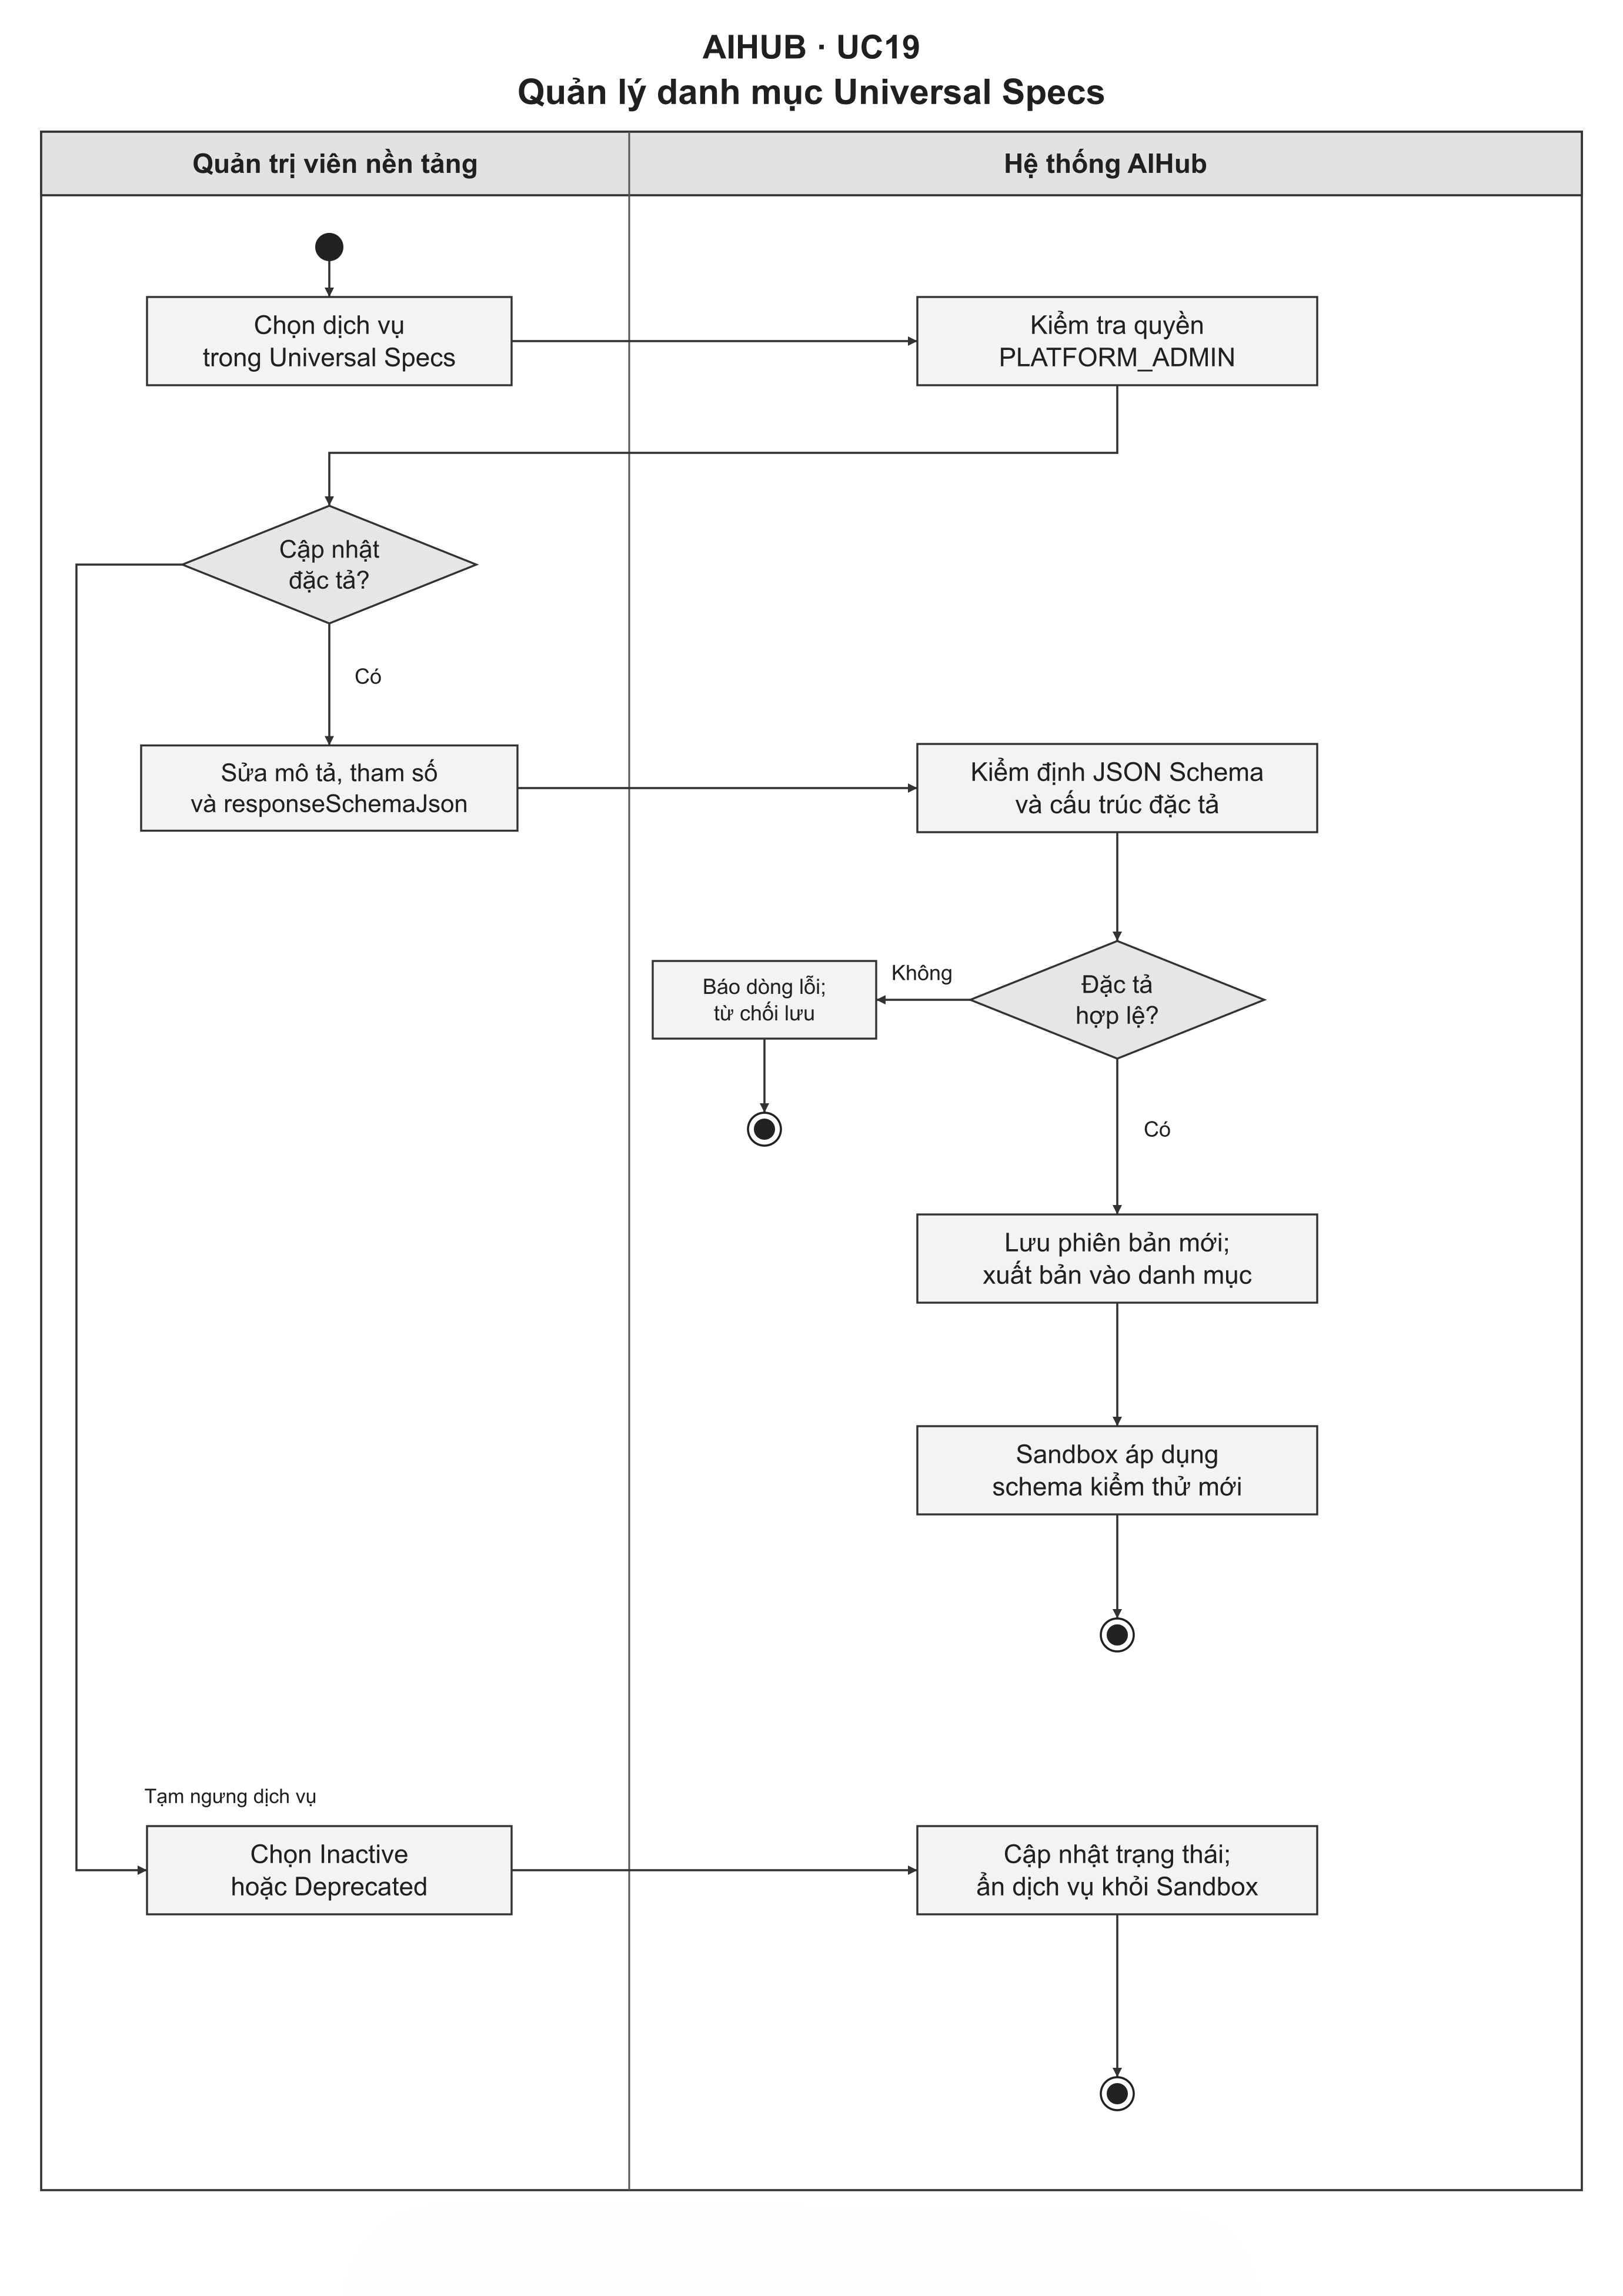
\includegraphics[width=\linewidth,height=0.72\textheight,keepaspectratio]{Images/Activity/AIHub/activity_uc19_universal_specs.png}
    \caption{Sơ đồ hoạt động AIHub -- Use-case 19: Quản lý danh mục Universal Specs}
    \label{aihub:fig:activity_uc19}
    \label{aihub:fig:act_uc19_manage_universal_specs}
\end{figure}

Quản trị viên tạo hoặc cập nhật đặc tả dịch vụ. Danh mục và khả năng chạy thử trong Sandbox được cập nhật tương ứng.
% activity-generated:end


\clearpage

\paragraph{Luồng hoạt động: Kiểm toán hệ thống và truy vết giao dịch (Use-case 20)}

% activity-generated:start
\begin{figure}[H]
    \centering
    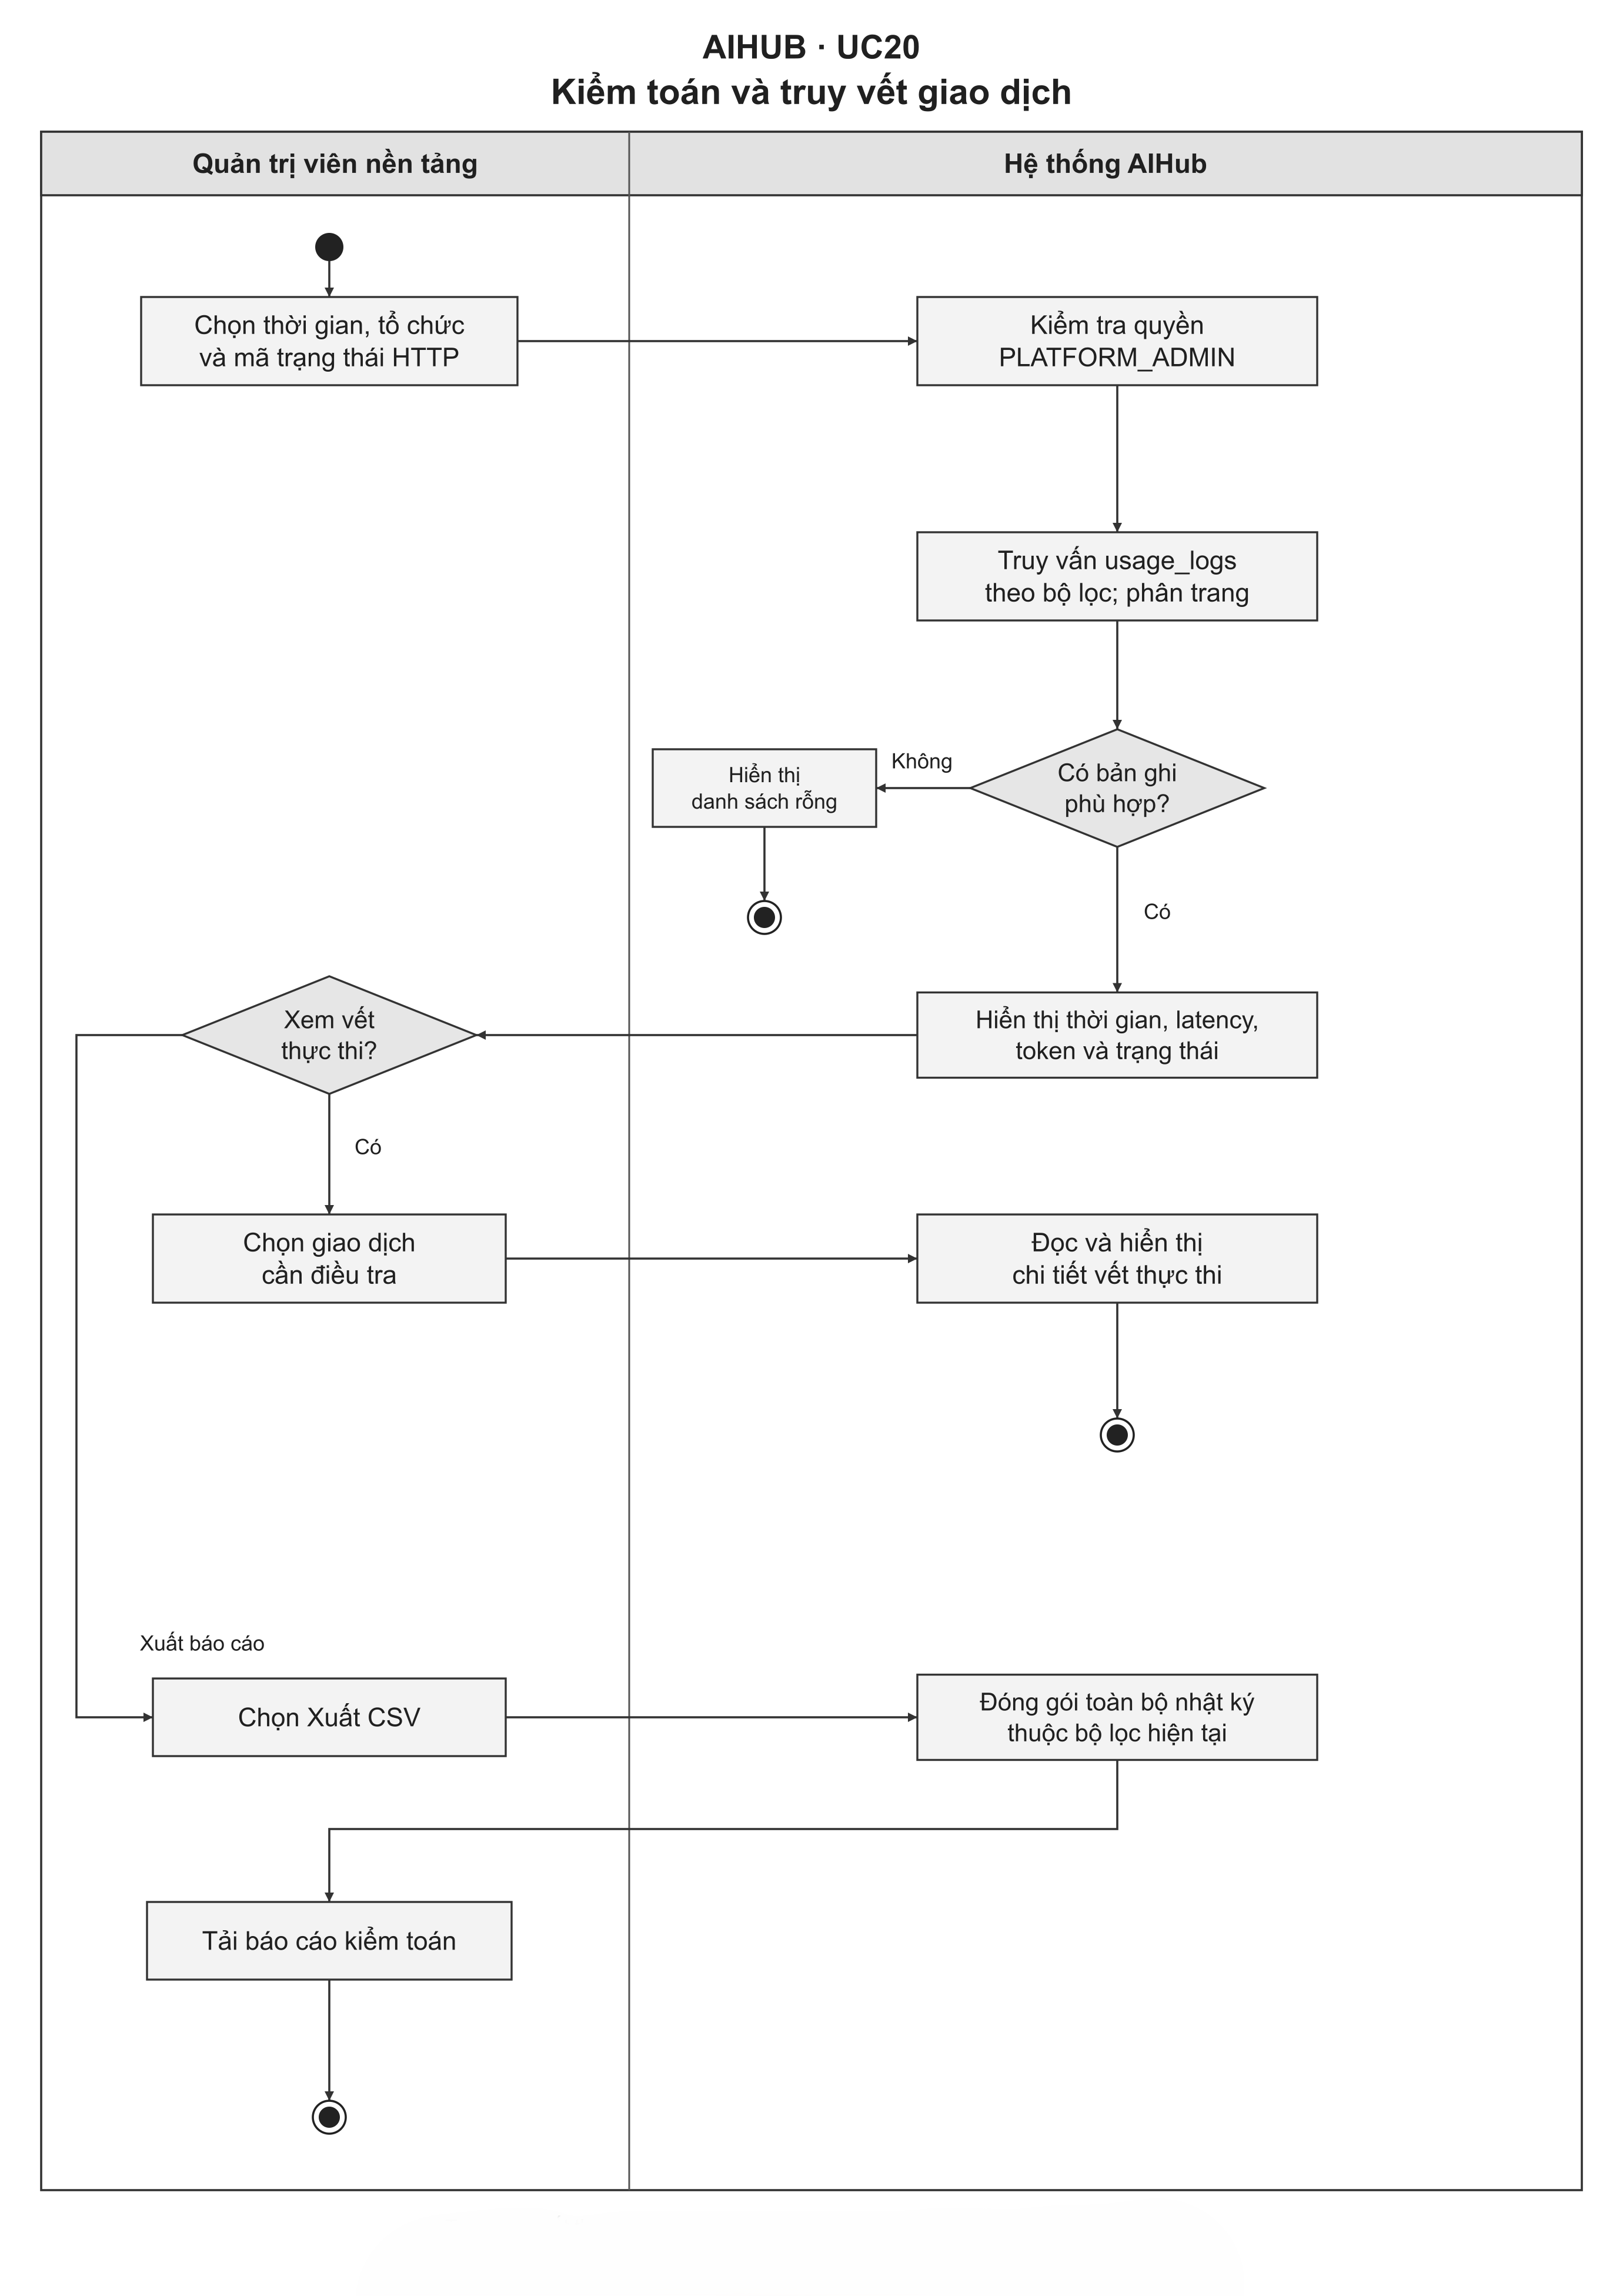
\includegraphics[width=\linewidth,height=0.72\textheight,keepaspectratio]{Images/Activity/AIHub/activity_uc20_audit_logs.png}
    \caption{Sơ đồ hoạt động AIHub -- Use-case 20: Kiểm toán và truy vết giao dịch}
    \label{aihub:fig:activity_uc20}
    \label{aihub:fig:act_uc20_system_audit_logs}
\end{figure}

Quản trị viên chọn tổ chức, thời gian và trạng thái cần tra cứu. Hệ thống hỗ trợ xuất CSV theo cùng phạm vi dữ liệu.
% activity-generated:end


\clearpage
\subsubsection{Sơ đồ luồng dữ liệu DFD}
\label{aihub:sec:dfd}

Phần này trình bày sơ đồ ngữ cảnh và DFD mức 1 của AIHub, tập trung vào dữ liệu xác thực API, sinh bài, thẩm định mẫu, cấu hình và giám sát. Backend, Gateway và các kho dữ liệu thuộc phạm vi hệ thống; nhà cung cấp AI và WISPACE Reference API là các tác nhân ngoài. Nguồn dẫn chứng Writing được phân biệt với dữ liệu bài nói của Wispace Speaking.

Luồng dữ liệu được tổ chức quanh các nhóm nghiệp vụ dưới đây. Mã E, P và D chỉ có ý nghĩa trong phạm vi từng hệ thống.

\begin{longtable}{|>{\raggedright\arraybackslash}p{0.07\linewidth}|>{\raggedright\arraybackslash}p{0.25\linewidth}|p{0.58\linewidth}|}
\caption{Tác nhân ngoài của AIHub}\label{aihub:tab:dfd-entities}\\
\hline
\textbf{Mã} & \textbf{Tác nhân} & \textbf{Dữ liệu trao đổi} \\
\hline
\endfirsthead
\hline
\textbf{Mã} & \textbf{Tác nhân} & \textbf{Dữ liệu trao đổi} \\
\hline
\endhead
E1 & Người dùng Portal & Gồm lập trình viên, chuyên viên học thuật, kỹ sư AI và quản trị viên. Cung cấp thông tin đăng nhập, yêu cầu thao tác và dữ liệu cấu hình; nhận kết quả theo quyền. \\
\hline
E2 & Ứng dụng tích hợp & Gửi credentials và payload gọi API; nhận bài tập, metadata sử dụng hoặc thông tin lỗi. Không mặc định đồng nhất ứng dụng này với mô-đun Speaking. \\
\hline
E3 & Nhà cung cấp AI & Gồm WISPACE AI Micro-Engine, Gemini và OpenAI. Nhận Prompt hoặc yêu cầu thăm dò; trả nội dung sinh, metadata hoặc trạng thái. Deterministic Engine nằm trong AIHub. \\
\hline
E4 & WISPACE Reference API & Nhận bộ lọc dẫn chứng lỗi viết; trả dữ liệu ngữ cảnh IELTS Writing hoặc thông tin lỗi kết nối. \\
\hline
\end{longtable}


\begin{longtable}{|>{\raggedright\arraybackslash}p{0.07\linewidth}|p{0.48\linewidth}|p{0.35\linewidth}|}
\caption{Tiến trình mức 1 của AIHub}\label{aihub:tab:dfd-processes}\\
\hline
\textbf{Mã} & \textbf{Tiến trình} & \textbf{Phạm vi} \\
\hline
\endfirsthead
\hline
\textbf{Mã} & \textbf{Tiến trình} & \textbf{Phạm vi} \\
\hline
\endhead
P1 & Xác thực Portal và quản lý khóa & UC01--UC02 \\
\hline
P2 & Kiểm thử và xử lý API sinh bài & UC03--UC05, UC07 \\
\hline
P3 & Truy vấn dẫn chứng và thẩm định mẫu & UC06, UC08--UC11 \\
\hline
P4 & Cấu hình Prompt, model và đặc tả & UC12--UC13, UC19 \\
\hline
P5 & Phân tích chất lượng và xuất dữ liệu & UC14--UC15 \\
\hline
P6 & Quản trị tổ chức và giám sát & UC05, UC16--UC18, UC20 \\
\hline
\end{longtable}


\begin{longtable}{|>{\raggedright\arraybackslash}p{0.07\linewidth}|p{0.25\linewidth}|p{0.58\linewidth}|}
\caption{Kho dữ liệu của AIHub}\label{aihub:tab:dfd-stores}\\
\hline
\textbf{Mã} & \textbf{Kho dữ liệu} & \textbf{Nội dung} \\
\hline
\endfirsthead
\hline
\textbf{Mã} & \textbf{Kho dữ liệu} & \textbf{Nội dung} \\
\hline
\endhead
D1 & Danh tính và tổ chức & Tài khoản, phiên Portal, thành viên, vai trò, tổ chức, clientId và mã băm khóa bí mật. \\
\hline
D2 & Cấu hình dịch vụ & Prompt có phiên bản, chuỗi dự phòng, Universal Specs, gói và cấu hình hạn mức theo tổ chức. \\
\hline
D3 & Usage và kiểm toán & Sử dụng quota, mã phản hồi, latency, token và dấu vết thay đổi phục vụ giám sát, đối soát. \\
\hline
D4 & Dữ liệu học thuật & Dẫn chứng cục bộ, Prompt gắn với mẫu, rawAiOutput, finalOutput, điểm, trạng thái, người duyệt và lý do từ chối. \\
\hline
\end{longtable}


\clearpage

\paragraph{Sơ đồ ngữ cảnh.}

Sơ đồ thể hiện toàn bộ AIHub như một tiến trình duy nhất; các mũi tên ghi rõ dữ liệu gửi đến và dữ liệu trả về cho từng tác nhân ngoài.

\begin{figure}[H]
\centering
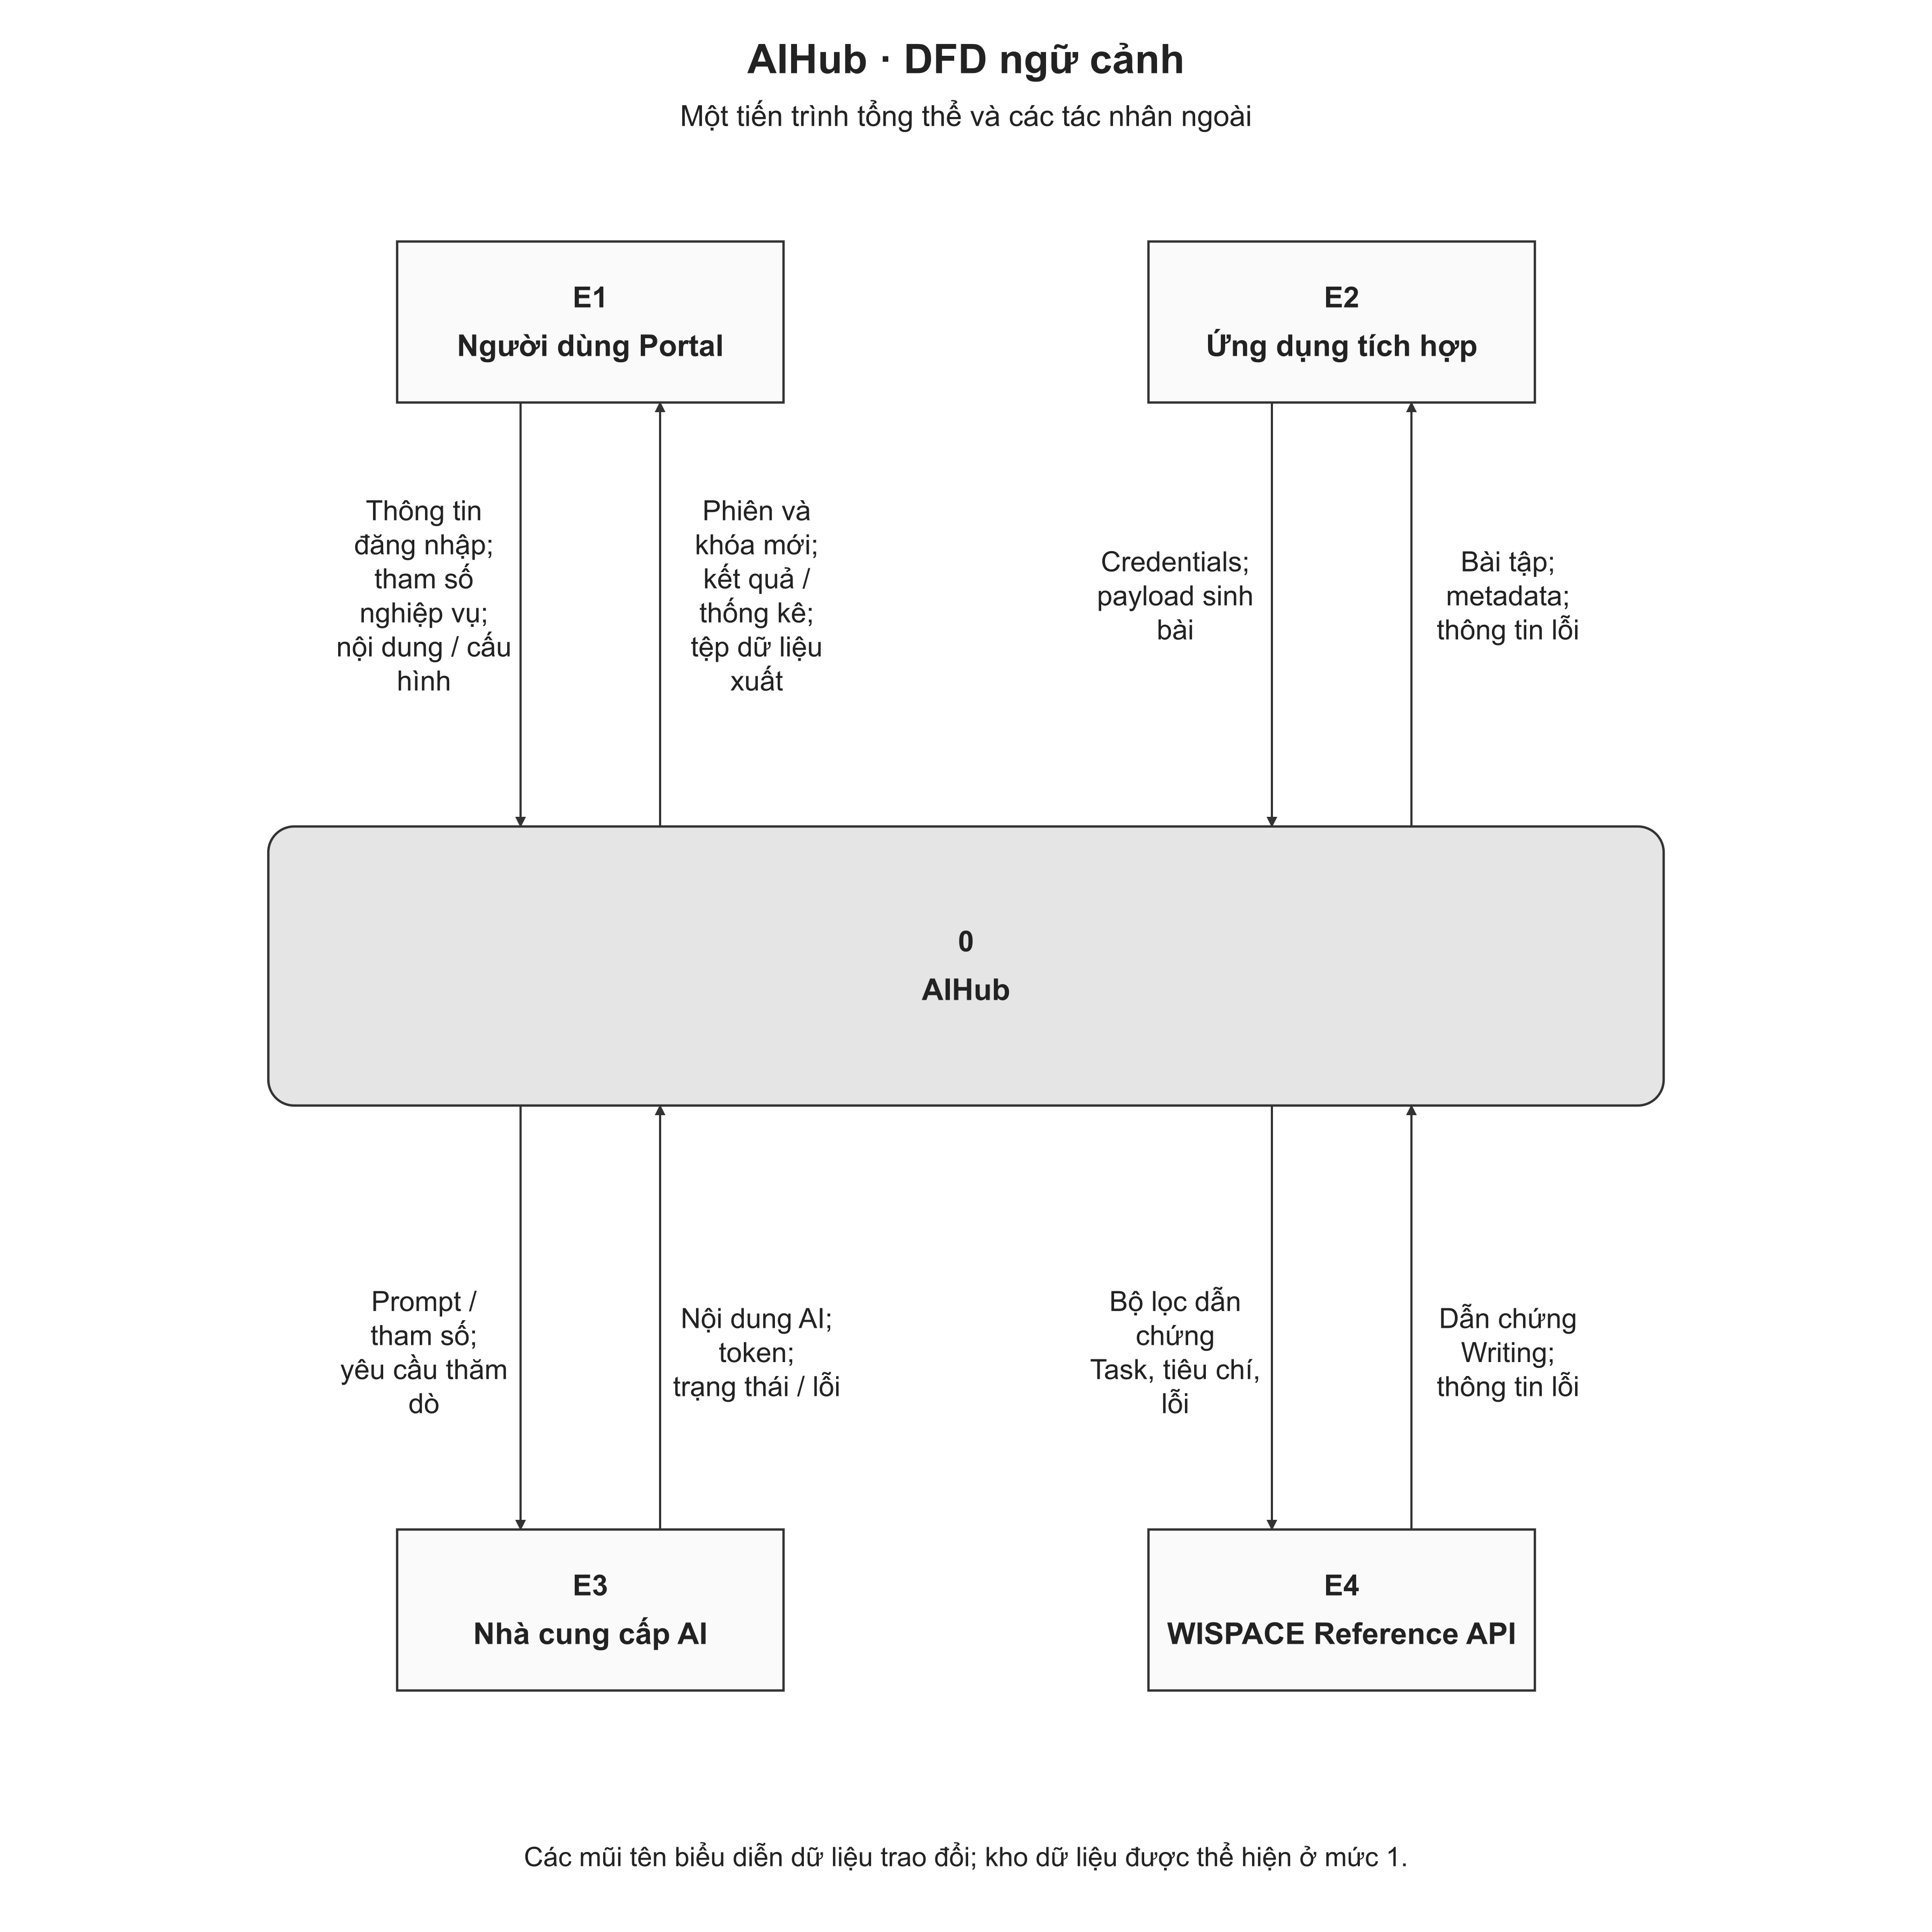
\includegraphics[width=\linewidth,height=0.78\textheight,keepaspectratio]{Images/DFD/AIHub/aihub_dfd_context.png}
\caption{DFD ngữ cảnh của AIHub}
\label{aihub:fig:dfd-context}
\end{figure}

\clearpage

\begin{longtable}{|p{0.22\linewidth}|p{0.72\linewidth}|}
\caption{Luồng dữ liệu biên của AIHub}\label{aihub:tab:dfd-boundary}\\
\hline
\textbf{Nguồn → Đích} & \textbf{Dữ liệu} \\
\hline
\endfirsthead
\hline
\textbf{Nguồn → Đích} & \textbf{Dữ liệu} \\
\hline
\endhead
E1 → 0 & Thông tin đăng nhập; tham số nghiệp vụ; nội dung / cấu hình \\
\hline
0 → E1 & Phiên và khóa mới; kết quả / thống kê; tệp dữ liệu xuất \\
\hline
E2 → 0 & Credentials; payload sinh bài \\
\hline
0 → E2 & Bài tập; metadata; thông tin lỗi \\
\hline
0 → E3 & Prompt / tham số; yêu cầu thăm dò \\
\hline
E3 → 0 & Nội dung AI; token; trạng thái / lỗi \\
\hline
0 → E4 & Bộ lọc dẫn chứng Task, tiêu chí, lỗi \\
\hline
E4 → 0 & Dẫn chứng Writing; thông tin lỗi \\
\hline
\end{longtable}


\paragraph{Sơ đồ mức 1.}

Để giữ nhãn và đường nối dễ đọc, cùng một sơ đồ mức 1 được trình bày thành hai phần. Các tác nhân và kho dữ liệu có cùng mã ở hai phần là cùng một đối tượng logic. Dữ liệu giữa các nhóm xử lý được trao đổi qua kho dùng chung, không phải các bản sao tách biệt.

\clearpage

\begin{figure}[H]
\centering
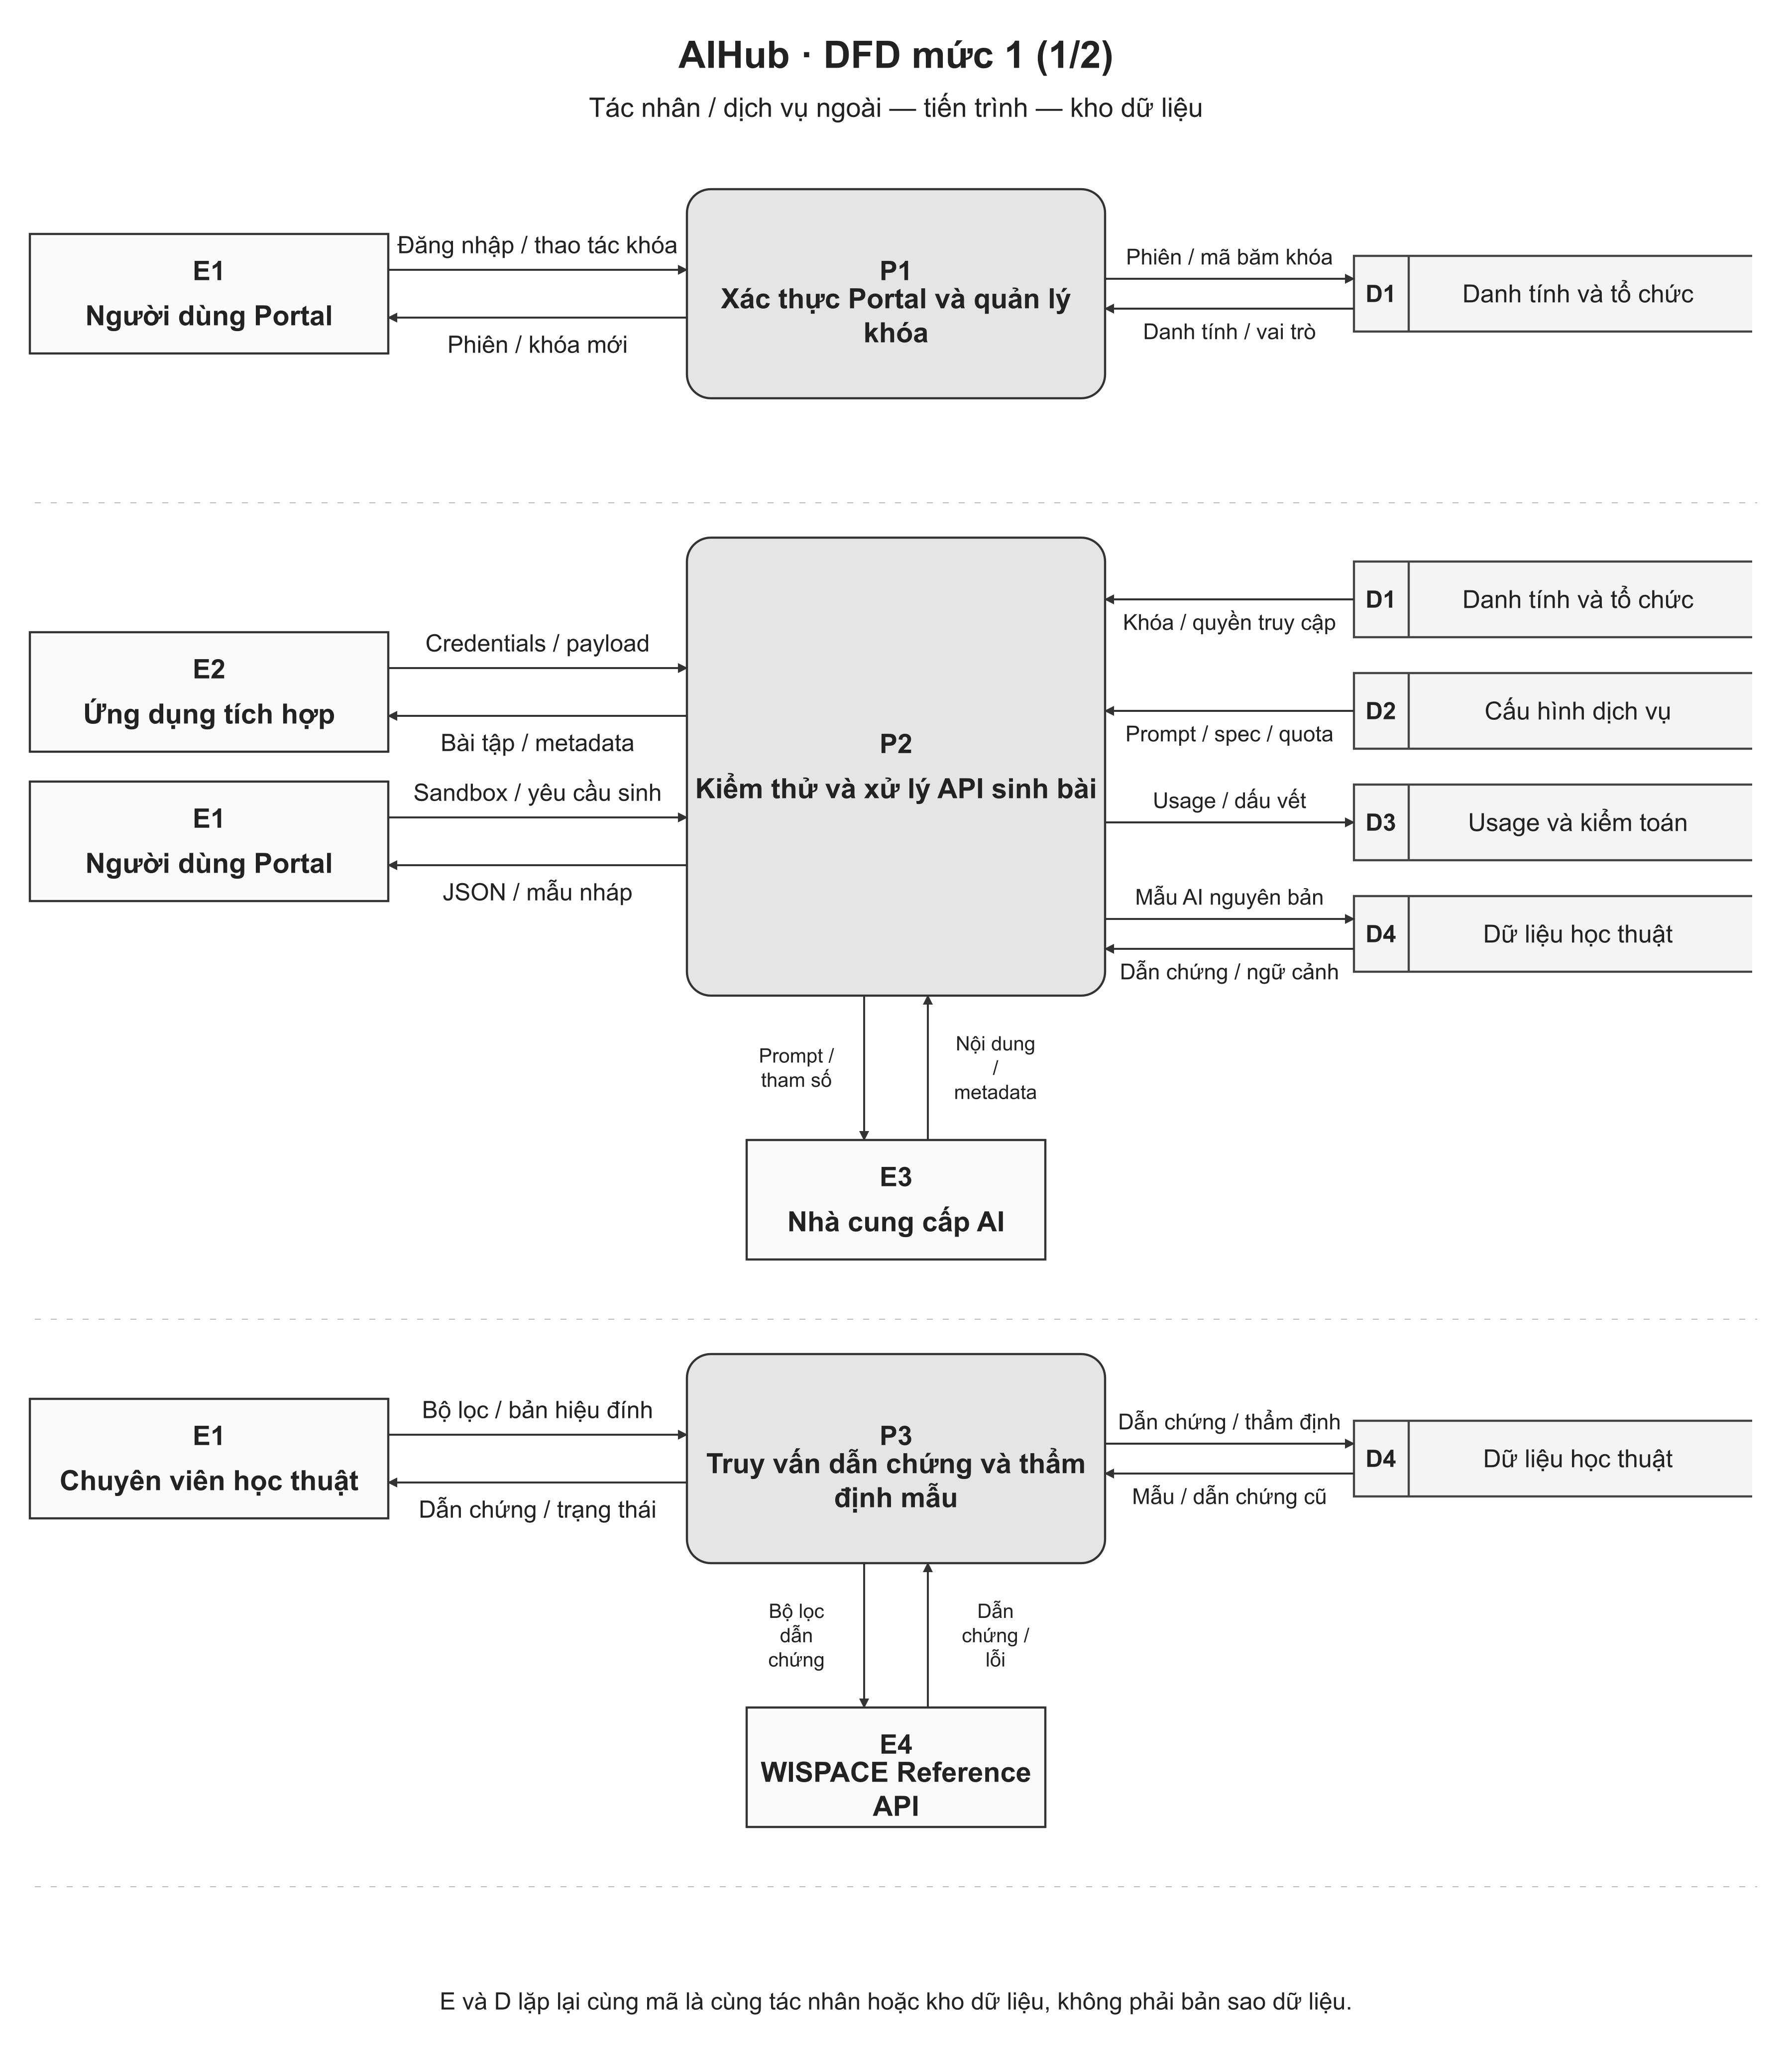
\includegraphics[width=\linewidth,height=0.78\textheight,keepaspectratio]{Images/DFD/AIHub/aihub_dfd_level1_1.png}
\caption{DFD mức 1 của AIHub: P1, P2, P3}
\label{aihub:fig:dfd-level1-1}
\end{figure}

\clearpage

\begin{figure}[H]
\centering
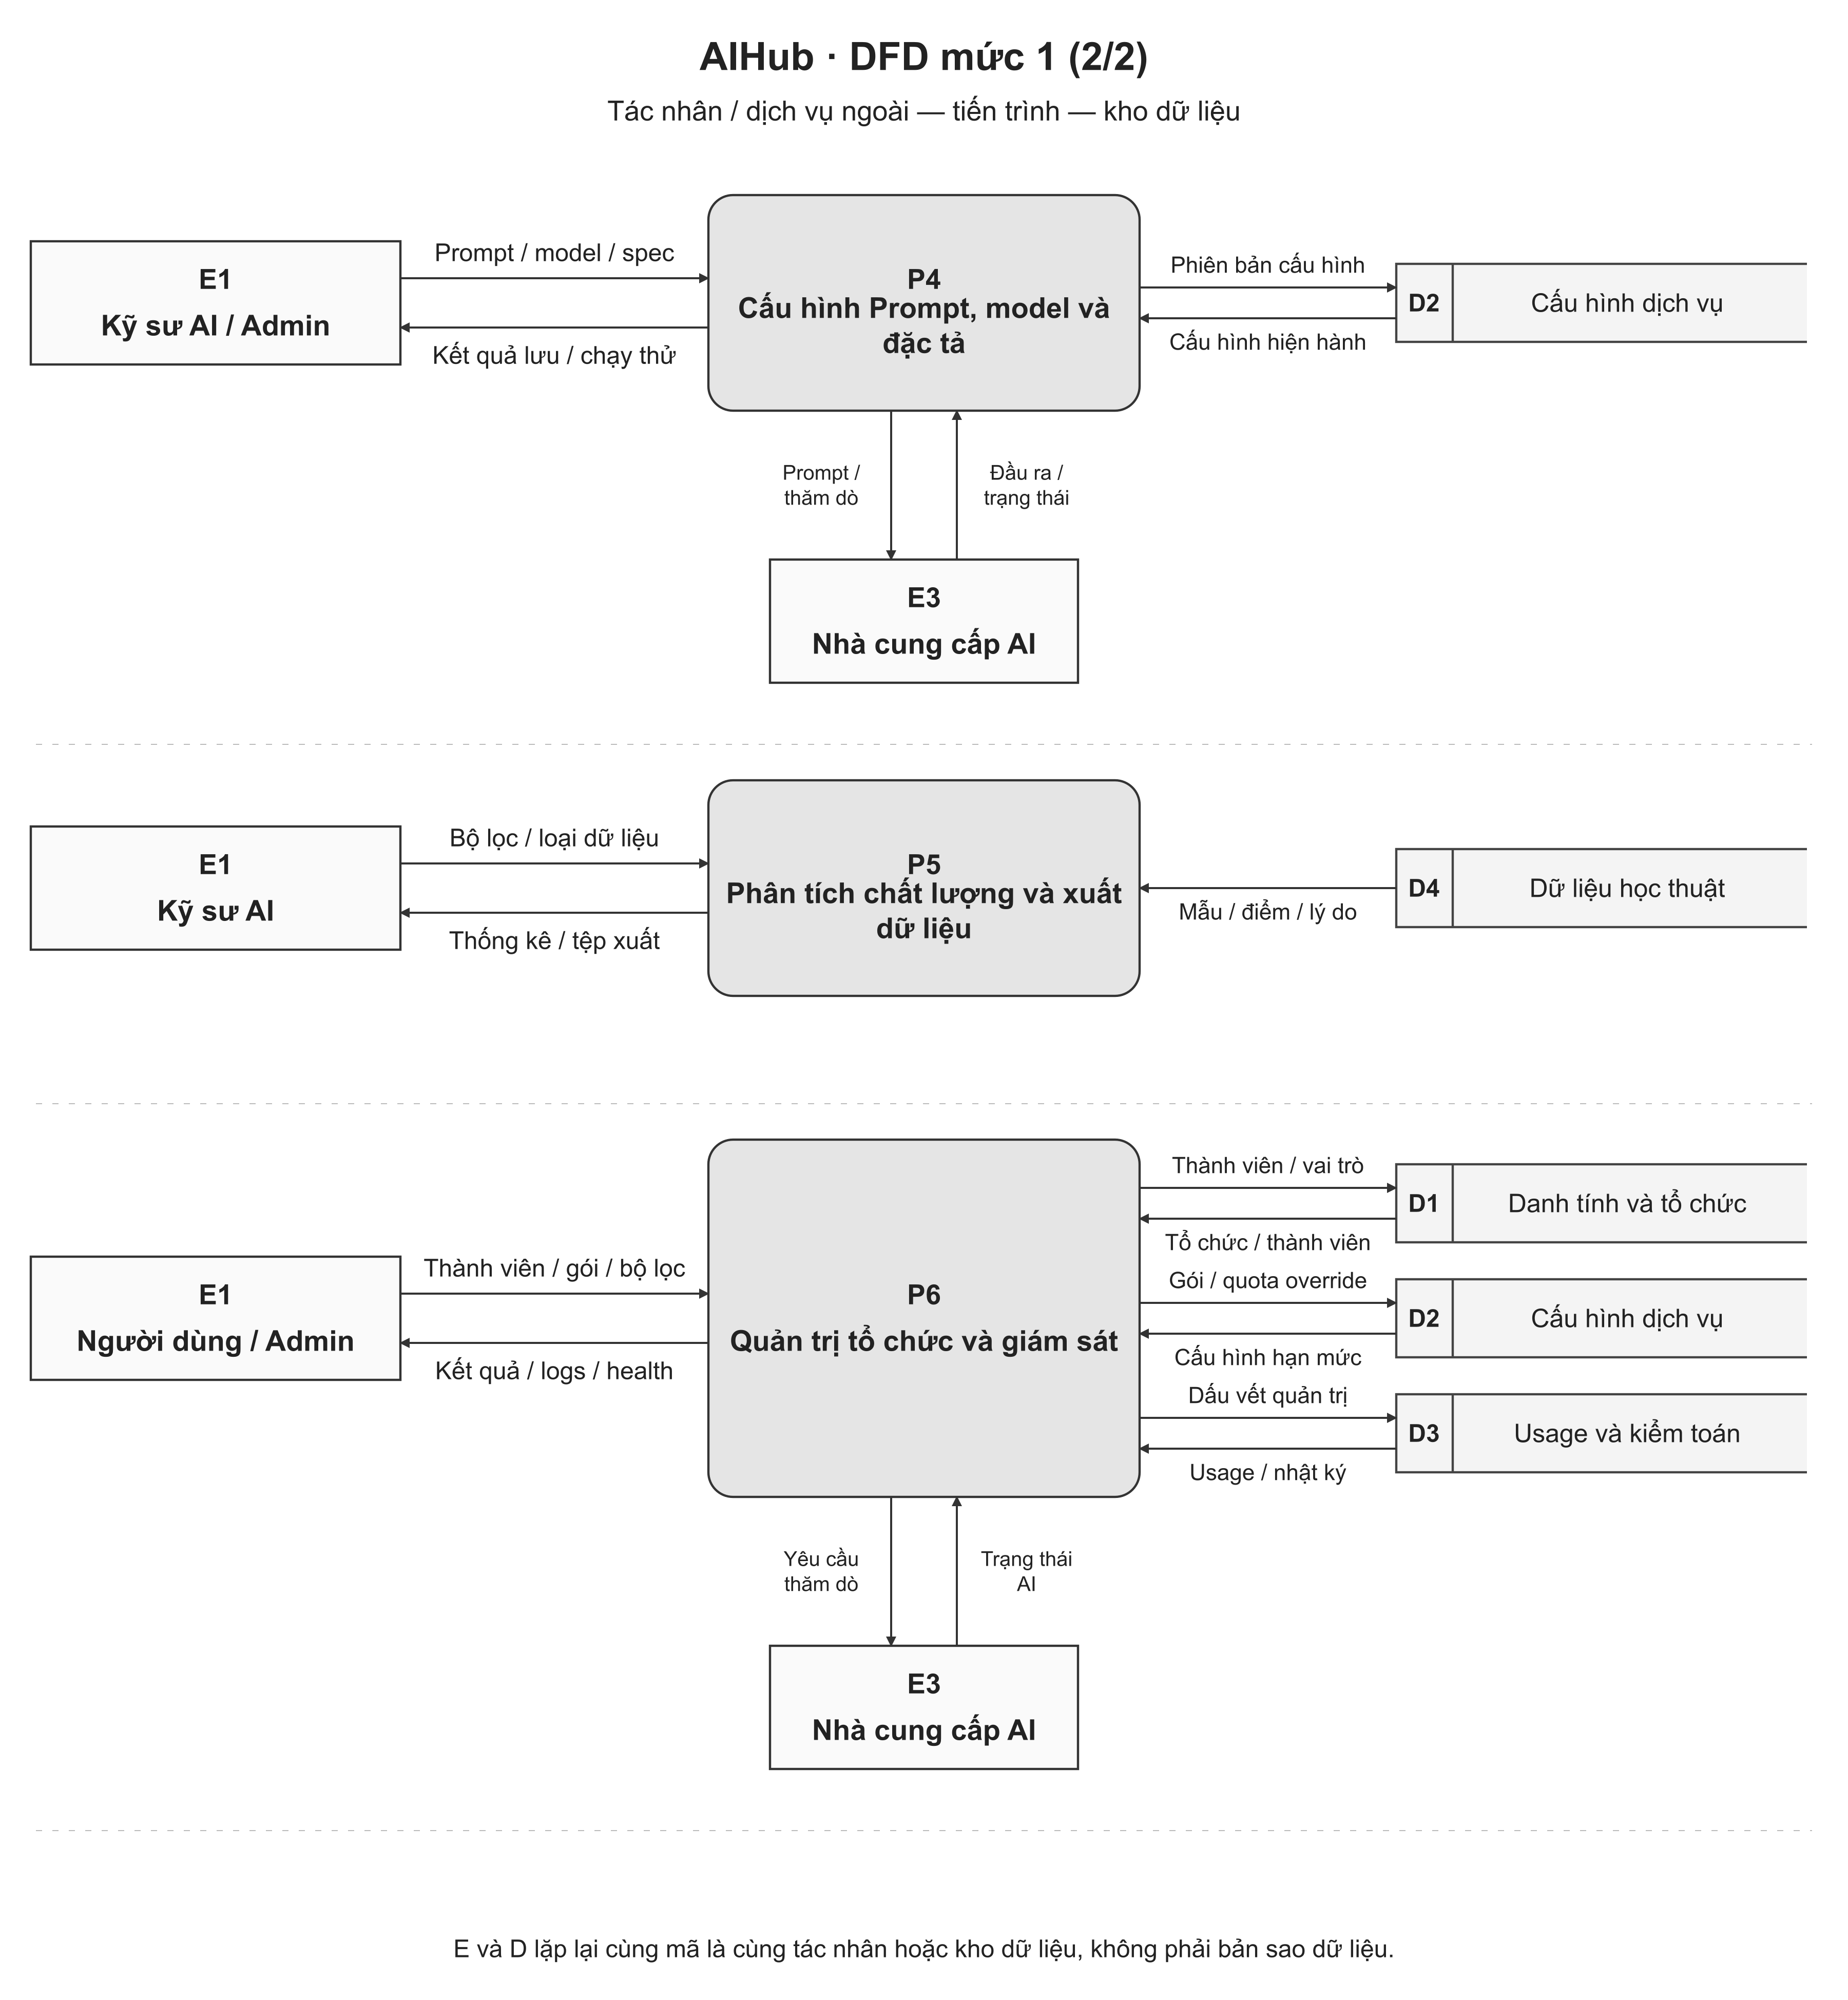
\includegraphics[width=\linewidth,height=0.78\textheight,keepaspectratio]{Images/DFD/AIHub/aihub_dfd_level1_2.png}
\caption{DFD mức 1 của AIHub: P4, P5, P6}
\label{aihub:fig:dfd-level1-2}
\end{figure}

\clearpage

\begin{longtable}{|p{0.22\linewidth}|p{0.72\linewidth}|}
\caption{Luồng dữ liệu mức 1 của AIHub}\label{aihub:tab:dfd-flows}\\
\hline
\textbf{Nguồn → Đích} & \textbf{Dữ liệu} \\
\hline
\endfirsthead
\hline
\textbf{Nguồn → Đích} & \textbf{Dữ liệu} \\
\hline
\endhead
E1 → P1 & Đăng nhập / thao tác khóa \\
\hline
P1 → E1 & Phiên / khóa mới \\
\hline
P1 → D1 & Phiên / mã băm khóa \\
\hline
D1 → P1 & Danh tính / vai trò \\
\hline
E2 → P2 & Credentials / payload \\
\hline
P2 → E2 & Bài tập / metadata \\
\hline
E1 → P2 & Sandbox / yêu cầu sinh \\
\hline
P2 → E1 & JSON / mẫu nháp \\
\hline
D1 → P2 & Khóa / quyền truy cập \\
\hline
D2 → P2 & Prompt / spec / quota \\
\hline
P2 → D3 & Usage / dấu vết \\
\hline
P2 → D4 & Mẫu AI nguyên bản \\
\hline
D4 → P2 & Dẫn chứng / ngữ cảnh \\
\hline
P2 → E3 & Prompt / tham số \\
\hline
E3 → P2 & Nội dung / metadata \\
\hline
E1 → P3 & Bộ lọc / bản hiệu đính \\
\hline
P3 → E1 & Dẫn chứng / trạng thái \\
\hline
P3 → D4 & Dẫn chứng / thẩm định \\
\hline
D4 → P3 & Mẫu / dẫn chứng cũ \\
\hline
P3 → E4 & Bộ lọc dẫn chứng \\
\hline
E4 → P3 & Dẫn chứng / lỗi \\
\hline
E1 → P4 & Prompt / model / spec \\
\hline
P4 → E1 & Kết quả lưu / chạy thử \\
\hline
P4 → D2 & Phiên bản cấu hình \\
\hline
D2 → P4 & Cấu hình hiện hành \\
\hline
P4 → E3 & Prompt / thăm dò \\
\hline
E3 → P4 & Đầu ra / trạng thái \\
\hline
E1 → P5 & Bộ lọc / loại dữ liệu \\
\hline
P5 → E1 & Thống kê / tệp xuất \\
\hline
D4 → P5 & Mẫu / điểm / lý do \\
\hline
E1 → P6 & Thành viên / gói / bộ lọc \\
\hline
P6 → E1 & Kết quả / logs / health \\
\hline
P6 → D1 & Thành viên / vai trò \\
\hline
D1 → P6 & Tổ chức / thành viên \\
\hline
P6 → D2 & Gói / quota override \\
\hline
D2 → P6 & Cấu hình hạn mức \\
\hline
P6 → D3 & Dấu vết quản trị \\
\hline
D3 → P6 & Usage / nhật ký \\
\hline
P6 → E3 & Yêu cầu thăm dò \\
\hline
E3 → P6 & Trạng thái AI \\
\hline
\end{longtable}


P3 lưu dẫn chứng vào D4 để P2 sử dụng khi sinh nội dung. Mẫu nguyên bản do P2 ghi vào D4 được P3 hiệu đính và thẩm định; P5 chỉ trích xuất dữ liệu phù hợp với loại tập huấn luyện được chọn. P2 và P6 cùng sử dụng D3 cho nhật ký và đối soát hạn mức. Sandbox của dịch vụ đối tác dùng dữ liệu mô phỏng trong P2, không phát sinh một lời gọi thật đến đối tác.

Deterministic Engine là thành phần dự phòng nội bộ của P2. Health check trong P6 kiểm tra kho dữ liệu nội bộ và nhận trạng thái từ nhà cung cấp AI; không xem PostgreSQL như một tác nhân ngoài.

Các luồng dữ liệu biên ở sơ đồ ngữ cảnh được phân bổ vào các tiến trình mức 1 tương ứng. Luồng đọc, ghi và phản hồi được thể hiện bằng các mũi tên riêng; sơ đồ không dùng điều kiện rẽ nhánh, nút bắt đầu hoặc kết thúc của activity diagram.


\subsection*{Kết chương}
Chương này đã phân tích các use-case, luồng hoạt động và luồng dữ liệu của Wispace Speaking và AIHub. Các mô hình xác định trách nhiệm của tác nhân, dữ liệu đầu vào, kết quả xử lý và các kho lưu trữ, làm cơ sở cho thiết kế và hiện thực hệ thống ở các chương tiếp theo.
